%% ut-thesis.tex -- document template for graduate theses at UofT
%%
%% Copyright (c) 1998-2013 Francois Pitt <fpitt@cs.utoronto.ca>
%% last updated at 16:20 (EDT) on Wed 25 Sep 2013
%%
%% This work may be distributed and/or modified under the conditions of
%% the LaTeX Project Public License, either version 1.3c of this license
%% or (at your option) any later version.
%% The latest version of this license is in
%%     http://www.latex-project.org/lppl.txt
%% and version 1.3c or later is part of all distributions of LaTeX
%% version 2005/12/01 or later.
%%
%% This work has the LPPL maintenance status "maintained".
%%
%% The Current Maintainer of this work is
%% Francois Pitt <fpitt@cs.utoronto.ca>.
%%
%% This work consists of the files listed in the accompanying README.

%% SUMMARY OF FEATURES:
%%
%% All environments, commands, and options provided by the `ut-thesis'
%% class will be described below, at the point where they should appear
%% in the document.  See the file `ut-thesis.cls' for more details.
%%
%% To explicitly set the pagestyle of any blank page inserted with
%% \cleardoublepage, use one of \clearemptydoublepage,
%% \clearplaindoublepage, \clearthesisdoublepage, or
%% \clearstandarddoublepage (to use the style currently in effect).
%%
%% For single-spaced quotes or quotations, use the `longquote' and
%% `longquotation' environments.


%%%%%%%%%%%%         PREAMBLE         %%%%%%%%%%%%

%%  - Default settings format a final copy (single-sided, normal
%%    margins, one-and-a-half-spaced with single-spaced notes).
%%  - For a rough copy (double-sided, normal margins, double-spaced,
%%    with the word "DRAFT" printed at each corner of every page), use
%%    the `draft' option.
%%  - The default global line spacing can be changed with one of the
%%    options `singlespaced', `onehalfspaced', or `doublespaced'.
%%  - Footnotes and marginal notes are all single-spaced by default, but
%%    can be made to have the same spacing as the rest of the document
%%    by using the option `standardspacednotes'.
%%  - The size of the margins can be changed with one of the options:
%%     . `narrowmargins' (1 1/4" left, 3/4" others),
%%     . `normalmargins' (1 1/4" left, 1" others),
%%     . `widemargins' (1 1/4" all),
%%     . `extrawidemargins' (1 1/2" all).
%%  - The pagestyle of "cleared" pages (empty pages inserted in
%%    two-sided documents to put the next page on the right-hand side)
%%    can be set with one of the options `cleardoublepagestyleempty',
%%    `cleardoublepagestyleplain', or `cleardoublepagestylestandard'.
%%  - Any other standard option for the `report' document class can be
%%    used to override the default or draft settings (such as `10pt',
%%    `11pt', `12pt'), and standard LaTeX packages can be used to
%%    further customize the layout and/or formatting of the document.

%% *** Add any desired options. ***
\documentclass{ut-thesis}
\usepackage{soul}
\usepackage{color}
\usepackage{hyperref}
\usepackage{pdfcomment}
\hypersetup{
    colorlinks=true,
    linkcolor=[rgb]{.4,.28,.49},
	citecolor=[rgb]{.4,.28,.49},
    filecolor=magenta, 
}
\usepackage{graphicx}
\usepackage{wrapfig}
\graphicspath{ {./images/} }   
\usepackage{jlcode}
\usepackage[utf8]{inputenc}
\usepackage{courier}
\usepackage{url}
\usepackage{minted}
\usepackage{fontspec}
\usepackage{placeins}

\usepackage[inkscapearea=page]{svg}

\usepackage[separate-uncertainty = true,multi-part-units=single]{siunitx}
\sisetup{output-exponent-marker=\ensuremath{\mathrm{e}}}

\usepackage{rotating}

\renewcommand{\chapterautorefname}{Chapter} 
\renewcommand{\sectionautorefname}{Section} 
\let\subsectionautorefname\sectionautorefname 
\let\subsubsectionautorefname\sectionautorefname

%% *** Add \usepackage declarations here. ***
%% The standard packages `geometry' and `setspace' are already loaded by
%% `ut-thesis' -- see their documentation for details of the features
%% they provide.  In particular, you may use the \geometry command here
%% to adjust the margins if none of the ut-thesis options are suitable
%% (see the `geometry' package for details).  You may also use the
%% \setstretch command to set the line spacing to a value other than
%% single, one-and-a-half, or double spaced (see the `setspace' package
%% for details).


%%%%%%%%%%%%%%%%%%%%%%%%%%%%%%%%%%%%%%%%%%%%%%%%%%%%%%%%%%%%%%%%%%%%%%%%
%%                                                                    %%
%%                   ***   I M P O R T A N T   ***                    %%
%%                                                                    %%
%%  Fill in the following fields with the required information:       %%
%%   - \degree{...}       name of the degree obtained                 %%
%%   - \department{...}   name of the graduate department             %%
%%   - \gradyear{...}     year of graduation                          %%
%%   - \author{...}       name of the author                          %%
%%   - \title{...}        title of the thesis                         %%
%%%%%%%%%%%%%%%%%%%%%%%%%%%%%%%%%%%%%%%%%%%%%%%%%%%%%%%%%%%%%%%%%%%%%%%%

%% *** Change this example to appropriate values. ***
\degree{Doctor of Philosophy}
\department{Cell and Systems Biology}
\gradyear{2020}
\author{Michael Mattocks}
\title{Computational Approaches to \textit{D. rerio} Retinal Organogenesis}

%% *** NOTEbb ***
%% Put here all other formatting commands that belong in the preamble.
%% In particular, you should put all of your \newcommand's,
%% \newenvironment's, \newtheorem's, etc. (in other words, all the
%% global definitions that you will need throughout your thesis) in a
%% separate file and use "\input{filename}" to input it here.


%% *** Adjust the following settings as desired. ***

%% List only down to subsections in the table of contents;
%% 0=chapter, 1=section, 2=subsection, 3=subsubsection, etc.
\setcounter{tocdepth}{3}
\setcounter{secnumdepth}{3}

%% Make each page fill up the entire page.
\flushbottom


%%%%%%%%%%%%      MAIN  DOCUMENT      %%%%%%%%%%%%

\begin{document}

%% This sets the page style and numbering for preliminary sections.
\begin{preliminary}

%% This generates the title page from the information given above.
\maketitle

%% There should be NOTHING between the title page and abstract.
%% However, if your document is two-sided and you want the abstract
%% _not_ to appear on the back of the title page, then uncomment the
%% following line.
%\cleardoublepage

%% This generates the abstract page, with the line spacing adjusted
%% according to SGS guidelines.
\begin{abstract}
Increasing integration of sophisticated statistical and computational techniques into the analysis of cell and molecular biological data has created many opportunities for explaining organogenic phenomena by numerical analysis. This thesis first examines the suitability of the most developed of these explanations for the development of the \textit{D. rerio} eye, the stochastic mitotic mode explanation (SMME) for retinal progenitor cell (RPC) function, and demonstrates that it is neither the best available explanation, nor theoretically defensible. It is shown that a deterministic alternative model is an improved explanation for the data, and that the SMME cannot explain postembryonic RPC function. These studies support earlier hypotheses of a linear progression of competency phases over the hypothesized ``stochastic'' nature of RPC lineage commitment.

A Bayesian model comparison framework, relying centrally on the Galilean Monte Carlo nested sampling algorithm for estimation of model evidence and posterior parameter distributions, is subsequently elaborated as an improved method for testing models in organogenesis. The utility of this approach is proved by comparing models of \textit{D. rerio} RPC populations in the postembryonic Circumferential Marginal Zone (CMZ). The inferential framework is used to show that the activity of CMZ RPCs in the postembryonic period is best characterised by two distinct phases of proliferative activity with similar timing across morphological axes, despite asymmetrical population dynamics. Changes to RPC lineage commitment across the two phases suggest an explanation for the changing photoreceptor mosaic. These studies establish that CMZ RPCs are a dynamic population, whose postembryonic function is not adequately described as a recapitulation of an embryonic program.

Finally, the \textit{D. rerio} mutant \textit{rys} is shown to arise from a lesion in the npat locus, and the apparently paradoxically enlarged CMZ RPC population observed in these animals is demonstrated to arise from a failure of these cells to specify and exit the proliferative niche, and not from a proliferative defect. Nested sampling is used to prove that unique populations of nucleosome positions in \textit{rys} mutants and sibling arise from separate causal processes. A mechanism for these observations involving simultaneous changes to the subunit composition of the nucleosome pool and loss of translational control is advanced.

%% *** Put your Abstract here. ***
%% (At most 150 words for M.Sc. or 350 words for Ph.D.)
\end{abstract}

%% Anything placed between the abstract and table of contents will
%% appear on a separate page since the abstract ends with \newpage and
%% the table of contents starts with \clearpage.  Use \cleardoublepage
%% for anything that you want to appear on a right-hand page.

%% This generates a "dedication" section, if needed -- just a paragraph
%% formatted flush right (uncomment to have it appear in the document).
\begin{dedication}
This work is dedicated to the memory of my brother Gareth Akerman.
% *** Put your Dedication here. ***
\end{dedication}

%% The `dedication' and `acknowledgements' sections do not create new
%% pages so if you want the two sections to appear on separate pages,
%% uncomment the following line.
%\newpage  % separate pages for dedication and acknowledgements

%% Alternatively, if you leave both on the same page, it is probably a
%% good idea to add a bit of extra vertical space in between the two --
%% for example, as follows (adjust as desired).
\vspace{.5in}  % vertical space between dedication and acknowledgements

%% This generates an "acknowledgements" section, if needed
%% (uncomment to have it appear in the document).
\begin{acknowledgements}
The completion of this thesis was possible only due to three teachers: my supervisor Dr. Vince Tropepe, who supported it with beatific patience and generosity, my advisor Dr. Umar Faruq Abdullah, who taught me that my scientific problems were in fact metaphysical and gave me the courage to proceed, and my sifu Liz Parry, who taught me how to stand and breathe in a fight. It further required the longsuffering care of my lovely wife Wing. I am indebted in innumerable ways to members, past and present, of the Tropepe, Bruce, Tepass, and Godt labs, as well as to other 6th floor denizens and the broader CSB community. I am particularly indebted to Monica Dixon and Loksum Wong for their extensive teachings and careful scientific example. Henry Hong and Audrey Darabie helped in innumerable ways with the imaging work and were a consistent source of encouragement and good cheer. All of the data generated here relied on the contributions of many hands, not least of which are the many involved with the long hours in care and feeding of the fish. I have gratefully included experimental work entirely generated by Monica Dixon and Maria Augusta Sartori in \autoref{chap:rys}; the underlying mapping work was performed by Jason Willer of . I am finally indebted to Dr. John Skilling, both for delivering me to a coherent statistical understanding in his published work, and for a generous response to an 11th-hour email which enabled me to complete \path{GMC_NS.jl} and to use it extensively in the final analyses.
\end{acknowledgements}

%% This generates the Table of Contents (on a separate page).
\tableofcontents

%% This generates the List of Tables (on a separate page), if needed
%% (uncomment to have it appear in the document).
\listoftables

%% This generates the List of Figures (on a separate page), if needed
%% (uncomment to have it appear in the document).
\listoffigures

%% You can add commands here to generate any other material that belongs
%% in the head matter (for example, List of Plates, Index of Symbols, or
%% List of Appendices).

%% End of the preliminary sections: reset page style and numbering.
\end{preliminary}


%%%%%%%%%%%%%%%%%%%%%%%%%%%%%%%%%%%%%%%%%%%%%%%%%%%%%%%%%%%%%%%%%%%%%%%%
%%  Put your Chapters here; the easiest way to do this is to keep     %%
%%  each chapter in a separate file and `\include' all the files.     %%
%%  Each chapter file should start with "\chapter{ChapterName}".      %%
%%  Note that using `\include' instead of `\input' will make each     %%
%%  chapter start on a new page, and allow you to format only parts   %%
%%  of your thesis at a time by using `\includeonly'.                 %%
%%%%%%%%%%%%%%%%%%%%%%%%%%%%%%%%%%%%%%%%%%%%%%%%%%%%%%%%%%%%%%%%%%%%%%%%

%% *** Include chapter files here. ***
\section*{Introductory Notes}
\label{ch:intro}
\addcontentsline{toc}{chapter}{\nameref{ch:intro}}

\subsection*{Thesis Guide}
This document is split into three parts. Part I contains results and discussion pertaining to empirical modelling studies that will be of interest to committee members and developmental biologists. Readers wishing to confine themselves to results chapters should examine \autoref{chap:SMME}, \autoref{chap:CMZ}, and \autoref{chap:rys}. Part II contains technical reports pertaining to novel software that was written in order to perform the analyses presented in Part I. Part III contains supplementary materials arising from Parts I and II. These include detailed descriptions of the methods used in Part I, less-technical explanations of relevant statistical and model theory, the source code of all software and analyses, and the bibliography. The source code has been omitted from the print document.

Synopses have been provided in italics at the top of each chapter in Part I. These consist of numbered statements, which summarise the accordingly numbered section in the text.

Readers of the .pdf document will find some text highlighted in plum throughout the thesis. Section indices highlighted in this way link to the specified section.  Because empirical results in Part I are separated from relevant methods and code in Part III, links to the methods and code used to generate the figure's data and analysis are given in figure captions. Technical terms have also been highlighted when pertinent material is available in Part III to explain them for the reader who may be unfamiliar.

Readers who wish to replicate analyses, inspect datasets, etc., will find guidance in \autoref{chap:allsup}.

\subsection*{Terminology and Style}
Throughout \autoref{chap:RPCreview}, \autoref{chap:SMME}, and \autoref{chap:SMMEoutro}, I have used the apellation "Harris" when referring to the output of William Harris' research group. This is a large body of research spanning several decades, and involves many co-authors. My use of "Harris" here is a convenience, as Harris is the only common author across the period in question, and presumably the agent carrying these ideas forward from project to project. It is not intended to slight or minimize the contributions of any of the other members of Harris' group (many of whom are now senior scientists in their own right). I have used "Raff" in an identical sense in referring to Martin Raff research group's work in \autoref{chap:SMMEoutro}.

I have preferred the terms "specification", "determination", and their derivatives, to refer to cells assuming a particular lineage fate. "Differentiation" is well-understood, but ambiguous, and often understood to relate to the mitotic event itself, which I generally do not intend. "A cell has specified" means it has assumed a stable macromolecular identity or "fate". This term is intended to correspond exactly with the appearance of stable markers of cell type.

Unless otherwise noted, formatting of quoted material is preserved, so that italic emphases appear in the original.

\part{Modelling Studies}
\section*{Pr\'{e}cis of Modelling Studies}
\label{ch:precis}
\addcontentsline{toc}{chapter}{\nameref{ch:precis}}

The primary concern of this thesis is developing and assessing computational models of retinal progenitor cell (RPC) phenomena. While many different explanations for various aspects of eye development exist, these have usually been supported by assessing the frequentist significance of observed effects (i.e. t-testing), not by building formally testable models of the phenomena themselves. Of the explanations which could be subject to model comparison, virtually all of these are derivatives of the Simple Stochastic Model (SSM), dating to the earliest work, performed by Till and McCulloch \cite{Till1964}.

The explosion of molecular biological information has massively increased the number of parameters that might be included in RPC models. The question of how RPC activity might be successfully predicted and controlled in vivo may revolve around finding adequate models that explain retinogenetic processes. The development and assessment of such models is, therefore, of fundamental basic and applied interest. This is particularly so, in light of increasing interest in entraining RPCs for the purpose of retinal regenerative medicine. Our group is particularly interested in the possibility that RPCs located in the peripheral retinal annulus of the circumferential marginal zone (CMZ), which are present in zebrafish and mammals alike, could be harnessed for retinal repair.

It is surprising that, despite the use of SSMs, the literature on neural stem cells contains virtually no systematic statistical approaches to the construction, optimization, or comparison of models. This thesis is an attempt to address this problem. It proceeds in three basic strokes. Firstly, Chapters \ref{chap:RPCreview} and \ref{chap:SMME} evaluate the existing explanations of RPC behaviour, and find that those with formal model components are deficient, and cannot explain the activities of RPCs in the CMZ. Secondly, Chapters \ref{chap:SMMEoutro} and \ref{chap:CMZ} propose a general CMZ modelling framework under which the Bayesian evidence for different model-hypotheses might be assessed, and, by testing a variety of population-level hypotheses, provide guidance and develop the methods required to test cell-based hypotheses. Lastly, Chapters \ref{chap:rys} and \ref{chap:rysoutro} introduce the zebrafish CMZ mutant \textit{rys}, and apply some of the methods developed in the second stroke to explain aspects of the aberrant morphology and behaviour of \textit{rys} RPCs. 

\autoref{chap:RPCreview} begins by summarizing the range of explanations that have been offered for RPC activities, and introduces the primary set of formal models that have recently been used to favour an explanation centered around a supposed stochastic mitotic mode of RPCs. \autoref{chap:SMME} elucidates the structure and development of the stochastic mitotic mode explanation (SMME) models, finding fundamental logical errors in their interpretation of "stochasticity". Moreover, by pursuing a basic information theoretical model selection approach, it is demonstrated that the SMME is not even the best available explanation relying on this flawed notion of stochasticity.

\autoref{chap:SMMEoutro} discusses the implications of \autoref{chap:SMME} for models of RPCs generally, and in the CMZ particularly; it also recommends a better model selection approach from Bayesian theory, nested sampling. \autoref{chap:CMZ} surveys the activity of RPCs in the post-embryonic zebrafish CMZ, developing Bayesian methods for doing so. These methods include the use of nested sampling to solve the long-standing problem of estimating cell cycle parameters of subpopulations of cells from cumulative thymidine labelling measurements of the entire super-population. It concludes with recommendations for future modelling approaches to the CMZ, structured by the foregoing Bayesian analysis. 

 \autoref{chap:rys} identifies the causative mutation in \textit{rys} and shows that the zebrafish CMZ mutant \textit{rys} CMZ RPCs have disorganized chromatin, likely blocking differentiation but not proliferation. Nested sampling is used to demonstrate that the nuclear phenotype is likely the consequence of a shift in nucleosome histone composition in \textit{rys} progenitors. \autoref{chap:rysoutro} discusses some of the theoretical issues raised by the \textit{rys} analysis, and their implications for modelling retinogenesis more broadly, especially in integrating nuclear dynamics into models of RPCs.
\chapter{Canonical retinal progenitor cell phenomena and their explanations}
\chaptermark{Canonical RPC phenomena and their explanations}
\label{chap:RPCreview}

\section{The Harris Stochastic Mitotic Mode Explanation (SMME)}
The work presented in \autoref{chap:SMME} examines the best-developed theory of \textit{D. rerio} retinal progenitor cell (RPC) function. The theory in question is the work of pre\"{e}minent retinal biologist William Harris' research group, referred to hereafter Stochastic Mitotic Mode Explanation (SMME). This theory purports to explain the function of zebrafish RPCs in terms of stochastic effects on mitotic mode, which specifies the mitotic state and fate propensity of offspring.

The SMME for RPC function is of fundamental theoretical and practical interest. It is a concerted effort by the Harris group to explain how a complex tissue like a retina can arise from a field of similar proliferating cells. In 2009, Harris coauthored a detailed review chapter, documenting the bewildering array of macromolecules and cellular processes thought to be involved in RPC function \cite{Agathocleous2009}. This enumeration contains many caveats and notes that the effects of particular macromolecules routinely differ between developmental stages, cell types, organisms, and so forth. At this time, no clear, detailed, comprehensive models of RPC function had been advanced, and the review is typified by statements like ``It is difficult to reconcile all the studies on the initiation and spread of neurogenesis in a single model."\footnote{This was in no sense a problem with Harris' understanding. A similarly high-level review coauthored by Pam Raymond \cite{Adler2008} concluded, with regard to models of photoreceptor fate specification: ``The data reviewed in the preceding sections indicate that a ‘one-size-fits-all’ model is not possible..."} It is therefore remarkable that, over the next nine years, the Harris group would go on to promulgate a \hyperref[SSM]{simple stochastic model} of zebrafish RPC function invoking only two named macromolecules.

Harris thus seems to be making a bold attempt to cut the Gordian knot of conflicting explanatory threads and advance a simple, comprehensible, ``mind-sized" model of RPC function. Harris' explanation for zebrafish RPC function is a microcosm of the broader promise of ``Systems Biology" to make sense of the contemporary welter of conflicting datasets; by using sophisticated mathematical methods drawn from information and complexity theories, the apparent confusion will be clarified and underlying molecular mechanisms will be revealed. Given Harris' track record and pre\"{e}minence in the field, we have good reason to take seriously the possibility that he has succeeded. Examining whether this is the case is our first priority. To appreciate the scope of his theoretical maneuver, and possible alternatives to it, we begin by summarising the state of the art at the time of his 2009 review (as well as relevant subsequent additions).

\section{Explanations for RPC function in 2009 and the drive to unification}
\label{sec:TheoryOptions}
Molecular biologists have sought explanations for the same remarkable features of retinal progenitor cells for decades. Animal retinas, having well-understood functions and stereotyped structures, promise tractable  targets for typical molecular biological explanations. With well defined cell types present in tightly regulated proportions and topological organisations, both theoretically-inclined molecular biologists and clinically-inclined regenerative medical practitioners have found the retina to be a useful model tissue\footnote{Indeed, if central neuroregenerative medicine is to become a clinical possibility, it seems likely that the theoretical and practical issues are most likely to be resolved in eyes before other areas of the CNS.}. The regular, easily detected order in eyes seemed to suggest a similar level of order and regularity in the macromolecular processes which underlay the formation of the tissue. Older explanations commonly suggested that RPCs are more-or-less identical and go through rigidly stereotypical macromolecular processes. It is, however, the persistently observed departures from this conception that have occupied much of our attention.

The simplest explanation for the regularity of retinal development is that any given RPC is executing the same strict ``developmental program" as its neighbours. If every progenitor produces a similar number of cells, and the progeny are specified in similar proportions, well-understood principles of cellular adhesion could give rise to the characteristic laminar organisation observed in animal retinas. However, by the 1980s, vertebrate lineage tracing experiments revealed a surprising degree of inter-lineage variability in many neural progenitor systems, not least of which was the retina. In their seminal 1987 paper, David Turner and Connie Cepko, using retroviral lineage labelling techniques, demonstrated that individual RPC lineages in rats had diverse proliferative and fate specification outcomes \cite{Turner1987}; Harris' group confirmed this result in \textit{Xenopus} the subsequent year \cite{Holt1988}, suggesting this variability was a common feature of vertebrate RPC function.

Indeed, at this point, we find fairly clear accounts of what retinal biologists took their theoretical options to be in explaining this variability. As Harris' 1988 report states:

\begin{longquote}
Changes in cell character associated with cell type diversification may be controlled in an autonomous way, reflecting either a temporal program inside the cell (Temple and Raff, 1986), the asymmetrical segregation of cytoplasmic determinants (Strome and Wood,
1983; Sulston and Horvitz, 1977), stochastic events inside the cell (Suda et al., 1984), or some combination of
these processes. Alternatively, cell type may be controlled in a nonautonomous way, as in cases in which
the extracellular environment (Doupe et al., 1985) or
cellular interactions (Ready et al., 1976) elicit or limit cell
fate. With its multiplicity of cell types, the vertebrate nervous system would seem to require the ultimate sophistication in its means of cellular determination. 
\cite{Holt1988}
\end{longquote}

It is striking, then, that Harris' review of the literature two decades later describes the situation similarly:

\begin{longquote}
Once differentiation is initiated, regulatory
mechanisms within the retina ensure that progenitors retain the capacity to undergo more
divisions, in parallel with churning out differentiated cells, and that progenitors cease dividing at variable times. There is still debate
about the extent of early programming that allows progenitors to step through a series of
stereotypical divisions and the extent of regulation from within the whole retina. The production of differentiated cells alters the retinal
environment with time...

Moreover, cells from the same clone do not all
differentiate at the same time, suggesting three
possibilities: a stochastic mechanism for the
decision to differentiate, exposure of the two
daughters to different environments, or asymmetric inheritance of determinants.
\cite{Agathocleous2009}
\end{longquote}

In the same paper, he states that the ``simple structure and accessibility of the retina make it a useful model to study cell division and differentiation, and as a result most aspects of this have been studied, from lineage tracing of progenitors, to the morphological aspects of division, to the molecular mechanisms involved." Thus, by Harris' own account, some twenty years of additional research into almost every variety of macromolecular explanation for a huge range of RPC-related phenomena had not provided any means to narrow down the possibilities he had already laid out in 1988. We still have Raff's temporal program ("early programming ... step[ping] through a series of steretypical divisions"), asymmetric segregation of cytoplasmic inheritants during mitotic events, ``stochastic" events internal to the cells, and possible ``environmental" extracellular determinants. While the number of particular macromolecules functionally implicated in proliferative, specificative, and organisational RPC phenomena had greatly expanded, this had not provided any means to differentiate between these theoretical options. This is only one example of a general phenomenon, in which enumerationist research programs, directed at producing more and more facts about macromolecular involvement in cellular phenomena, have failed to generate additional theoretical understanding \cite{Kaneko2006}. Harris' SMME therefore represents an example of a ``Systems" biological explanation, in which biologists apply the analytical and interpretative methods of the physical and mathematical sciences in an effort to resolve the problems posed by biological complexity \cite{Morange2009}.

Before proceeding to the SMME itself, let us briefly summarise the diversity of phenomena implicated in RPC function by 2009, as well as the panoply of mechanisms offered as explanations. In doing so, it will become clear what has been elided in the SMME, and what may need to be restored in any alternative modelling approach.

\section{Canonical vertebrate RPC phenomena: the RPC ``morphogenetic alphabet"}

The bulk of our knowledge of RPC behaviour stems from histological observation employing a limited number of techniques. Simple observations of mitotic figures in a variety of animals had, by the 1950s, revealed the surprising diversity of RPC proliferative phenomena across vertebrate clades. However, it was the advent of lineage tracing techniques, particularly those marking single clonal lineages in whole retinae, and the extensive use of these techniques in the 1980s-90s, that formed most of the basic body of observations that any macromolecular explanation is now called upon to account for.

Since the majority of vertebrate retinas of biomedical interest are mammalian, and these retinae are fully formed in an early developmental period, RPC behaviour has been best-studied in an embryonic and early developmental context. Here, vertebrate RPCs are derived from the eye field population of the early neural plate and later neural tube. This population is separated into left and right eye primordia, which in turn pouch outwards toward the ectoderm, and, in conjunction with the lens placode (itself induced from the ectoderm), form the optic vesicle. The primitive eye is formed when this vesicle completes a complex morphological folding process, resulting in the cup-shaped structure of the retina \cite{Cavodeassi2018}. During this process, the cells of the neural retina are differentiated from the overlying retinal pigmented epithelium (RPE). Sometime after the formation of the retinal cup, RPCs begin to exit the cell cycle and are specified as retinal neurons. Studies of this early period revealed numerous difficult-to-explain features of RPC behaviour. Following Larsen's observation that tissue form is attributable to only six behaviours \cite{Larsen1992}, which she describes as the ``morphogenetic alphabet", I have categorised RPC phenomena as relating to proliferation, fate specification, migration, growth, death, and extracellular matrix formation. Since the vast majority of reported phenomena fall under the first two categories, proliferation and specification, these are given separate sections below, while those belonging to the last four are described collectively.

\subsection{Proliferative phenomena}

Clonal lineage tracing experiments reliably find that vertebrate RPCs give rise to highly variable numbers of offspring over the collective ``lifetime'' of the lineage. The most dramatic of these findings demonstrate that rat RPC lineage sizes vary across two orders of magnitude in vivo, from 1 to over 200 \cite{Turner1990}. While at least some of this variability must be related to differential integration of lineage markers into ``older" (giving fewer offspring) and ``newer" (giving more) RPCs, vertebrate RPC lineages nevertheless differ widely in their fecundity. The physical organisation of these clones is complex; as detailed below, RPC progeny may appear in any of the 3 retinal layers in a wide variety of specified fate combinations, and may engage in short-range migrations to appropriate positions for their specified fates. Most clonal lineages are ``extinguished"; that is, after some time, all of its members have become postmitotic. However, it has long been noted that not all cells produced by RPCs are strictly postmitotic neurons; specified M{\"u}ller glia retain the ability to reenter the cell cycle in response to stimuli (normally, retinal damage) \cite{Dyer2000,Fischer2003a}, and peripheral CMZ RPCs remain proliferative in those vertebrates whose eyes grow beyond early development (notably in frogs and fish, while the chick retina has a CMZ of more limited output \cite{Fischer2000}). Therefore, some clonal lineages may be organised into clumps associated with M{\"u}ller responses, while others in frogs and fish may continue to be ``plated out" in a more-or-less linear manner at the retinal periphery for as long as the lineage ``lives" \cite{Centanin2011}. This ongoing RPC contribution to peripheral neurogenesis has long been recognised, so that by 1954 we find the following statement introducing a study of unusual mitoses in the retina of a deepsea fish: 

\begin{longquote}
  It is conventional\footnote{Unfortunately, I am unable to locate the source of this convention, likely due to the poor preservation of many of these older reports. That this required no citation in 1954 suggests the original observations of CMZ proliferation may be in the early 20th century.} to hold that the growth of the vertebrate retina is only possible due to the presence, in this tissue, of a peripheral germinal zone. In this region, young elements actively multiply, and, by subsequent differentiation, give rise to the diverse nervous and sensory constituents of the retina.
  \cite{Vilter1954}
  
  [author's translation from the French]
\end{longquote}

Despite this, the proliferating RPCs in this ``peripheral germinal zone" (also known as the ``ciliary marginal zone", or CMZ, for its proximity to the retinal ciliary body) have not received the same level of attention as those associated with the central retina. As a consequence, these RPCs are generally treated as though they are a type of ``frozen" progenitor population, recapitulating spatially, along the peripheral-central axis, the process which RPCs in the central retina undergo in a time-dependent fashion\cite{Harris1998}.

The length of the RPC cell cycle is of considerable interest, since the evolution of this parameter in time, in conjunction with the RPC population size (the number of cells specified in the eye field), determines the eventual size of differentiated retinal neural population, and therefore the retina. RPC cell cycle length is usually inferred from clonal lineage size, although it has also been assayed directly in cumulative thymidine analogue labelling experiments \cite{Alexiades1996}. Vertebrate RPCs undergo a period of relative quiescence, in which the cell cycle lengthens, before the neural retina begins to be specified (in zebrafish, this period is ~16-24 hpf). The cell cycle shortens as RPCs begin to exit the cell cycle \cite{Harris1991,Li2000}. After the central retina is specified, the RPC cell cycle again lengthens, and is presumed to continue to slow until RPCs have completed specifying\footnote{This presumption is demonstrably incorrect in the \textit{D. rerio} eye, see \autoref{sec:sliceGMC} for a more plausible model of cell cycle dynamics in this organism.}.

Finally, the orientation of the RPC division plane in mitosis is also  implicated in retinal organisation. The orientation of divisions is associated with the both proliferation and fate specification of RPC progeny. For instance, interfering with spindle orientation in the developing rat retina, such that more RPC divisions occur parallel to the neuroepithelial plane (rather than along the apico-basal axis) results in more proliferative and fewer postmitotic, specified progeny\cite{Zigman2005}. That said, it seems that whatever effects are attributed to mitotic orientation are likely species-specific, as zebrafish RPCs display a different pattern of axis orientation, dividing mainly in the epithelial plane\cite{Das2003}.

\subsection{Fate specification phenomena}

Offspring of vertebrate RPC lineages may enter any of the three cellular layers of the retina. Moreover, single lineages can include any possible combination of cell fates, so that RPCs cannot be readily divided into ``types" on the basis of lineage fate outcomes \cite{Holt1988,Turner1990,Wetts1988}. While some progenitors have propensities to generate similar cell types, these relations seem species-specific, and may not define separate progenitor pools \cite{Adler2008}. In general, then, RPCs are taken to be totipotent with respect to the neural retina- all of the cell types\footnote{The ``cell type" concept is unusually well-defined in the retina, as there are an abundance of distinct morphological and molecular features which differentiate numerous subtypes of the seven general types of retinal neuron.} of the differentiated retina are derived from similar RPC lineages. Little about this picture has changed since its initial development, using a variety of lineage tracers (including retroviruses, thymidine analogues, and injectable dyes) and histochemical markers to supplement morphological identification of specified neurons. In particular, sophisticated modern live imaging experiments in zebrafish (many pioneered by Harris), have broadly confirmed the findings of the 80s and 90s in mammalian fixed specimens, explants, and live animals \cite{Boije2015}.

\label{Raff}
Of particular note are the observations of the Raff group \cite{Watanabe1990,Cayouette2003}, who demonstrated that dissociated rat RPCs, cultured at clonal density, took on morphological and histochemical features associated with different specified neural types in similar numbers and proportions, and on a similar schedule, to same-aged RPCs cultured in retinal explants. These results dramatically suggested that both the proliferative and fate specification behaviour of RPCs depends less on intercellular contact, and the complex signalling environment of the developing retina, than on factors intrinsic to the RPCs themselves. These studies contain the essential germ of Harris' eventual commitment to SSM explanations, purporting as they do to ``test the relative importance of cell-intrinsic mechanisms and extracellular signals in cell fate choice", and providing convincing evidence for the preponderant importance of the purported cell-intrinsic mechanisms.

\begin{figure}[!h]
  \makebox[\textwidth][c]{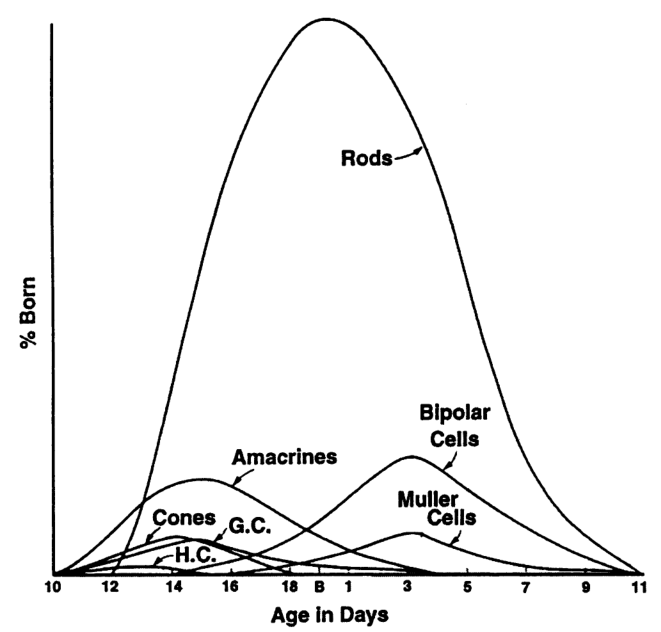
\includegraphics[width=.7\textwidth]{cepko0.png}}
  \caption{{\bf Histogenetic birth order of retinal neurons}}
  Adapted from \cite{Young1985} by \cite{Cepko1996}. G.C., Ganglion Cells; H.C., Horizontal Cells. Data from embryonic and perinatal mouse eyes.
  \label{horder}
\end{figure}

In spite of the apparent ability of RPCs to produce offspring specified to any of the possible neural cell fates, at any time during their lineage history\footnote{Even in papers arguing for a strict, linear sequence of specificative outcomes in all RPC lineages, the actual data show RPCs occasionally giving rise to ``late-born" photoreceptors subsequent to their first division\cite{Wong2009}, giving lie to the notion that the process is particularly strict.}, vertebrate retinal development displays a temporal ordering, such that in any particular location, retinal ganglion cells (RGCs) tend to be produced first, followed by the other cell types in what has been described as an overlapping ``histogenetic order", pictured in Figure \ref{horder}. As noted above, RPCs also exit the cell cycle in a spatiotemporally defined order (from central to peripheral over time), and specification follows the same pattern\footnote{In many studies, cell cycle exit is conflated with specification such that evidence of the former is taken as evidence of the latter. There are, however, reasons to believe cell cycle exit and specification are not the same process, discussed below.}. This naturally gave rise to questions about the origin of the ``overlap" observed in the sequential production of various cell types; conceptually, this overlap could be produced by identical RPCs executing identical rigid specification programs if they begin to execute it along the spatiotemporal gradient noted above, as originally suggested by Cepko et al. \cite{Cepko1996}. However, it is impossible to reconcile this notion with more recent results from Harris' \textit{in vivo} zebrafish lineage tracing studies \cite{Das2003,He2012,Boije2015}, which confirm mammalian cell culture work in demonstrating that vertebrate RPC lineages do not execute similar specificative programs. More recent articulations of Cepko's concept of linear specification programs incorporate variable sub-programs to account for this \cite{Cepko2014}.

\subsection{Other morphogenetic phenomena}
The outcomes of RPC proliferation and lineage commitment are often taken as sufficient explanation for the formation of the neural retina. Indeed, after the eye cup has been formed (prior to the specification of any neurons), RPCs are, in effect, already ``in place". Therefore, there are few documented RPC phenomena outside of the ``proliferation" and ``specification" categories of the morphogenetic alphabet \cite{Larsen1992}, which ennumerates the cellular processes contributing to tissue form and structure. RPCs do not seem inclined to migrate long distances , they seem not to generate much in the way of extracellular material\footnote{The formation of a laminin-rich basement membrane seems to be necessary for optic vesicle formation \cite{Ivanovitch2013}, but it is not clear that RPCs produce this. ECM function in eye formation remains under-studied.}, and, in non-pathological conditions, they are rarely seen to die. Still, there are a number of phenomena which appear to be important for proper retinal organisation that fall into these other ``alphabet" categories.

The most notable of these is interkinetic nuclear migration (INM), in which RPC nuclei move back and forth between the apical and basal surfaces of the retina. Common in many neural tissues, INM affects both proliferation and fate specification, but is dissociable from them- both cell cycle and specification proceed (albeit in a precocious manner) when INM is disrupted\cite{Murciano2002}. The apical retinal surface provides a microenvironment which appears to be required for RPC mitosis to occur\footnote{Nonapical divisions do occur, notably in specified, but proliferative cells \cite{Godinho2007}. The extent to which RPCs depend on the apical surface may depend on how ``RPC" is defined. In general, RPCs are no longer considered as such when they acquire characters associated with differentiated neurons (cell type markers, morphological traits, etc.), although it is clear that the acquisition of these characters does not necessarily imply that the cell is postmitotic. Any complete explanation of how RPCs give rise to the structure of the eye must also consider these nonapical divisions.}, and INM seems to consist of a directed, probably actomyosin-mediated movement to the apical surface, followed by an undirected ``random walk" away from the apical surface and hence toward the basal retina \cite{Norden2009}. This ``random walk" may arise from displacements due to the directed INM of neighbouring progenitors \cite{Azizi2020}. More committed RPCs also appear to actively migrate to positions appropriate for the specified cell type \cite{Chow2015,Icha2016}, although it is unclear if this short-range migration is caused by INM undergone by more actively proliferating progenitors. It seems likely that these short-range migrations of more specified cells are especially significant in the early retina, before the neural plexiform layers (consisting of axons and other neural processes) have begun to divide the cellular layers into bounded compartments.

Notable lacunae in the study of the RPC ``morphogenetic alphabet'' include the regulation of cell size and growth, and potential roles for cell death, both of which have received little attention. While cell size and growth are tightly linked to proliferative behaviour in yeast \cite{Yang2011}, any related effects in RPCs have not been elucidated. This may be a significant oversight, given the requirement for RPCs to continuously grow during their proliferative lifespan. Cell death does not seem to play the same ``pruning" role for RPCs that it often does in other neural tissues, and observed rates of cell death in normal RPC populations are very low, so few studies have been conducted.

\section{Macromolecular mechanistic explanations for RPC phenomena}

Having surveyed the cellular phenomena pertaining to RPC function in retinal development, we proceed to a selection of the many macromolecular mechanistic explanations (MEx) \cite{Fagan2012} that have been offered to explain them. Unsurprisingly, given the field's focus on the early events of eye development, these MEx are mainly targeted at this period. Thus, the majority explain tissue-level phenomena like the initial ``wave" of cell cycle exit and specification, without necessarily seeking a global explanation for RPC behaviour irrespective of context, so it is unknown how many of these might pertain to ongoing peripheral neurogenesis or other, adult neurogenic phenomena like those exhibited by M{\"u}ller glia. That said, we now turn to examine some of the best-developed of these explanations.

\subsection{Transcription factor networks}

Perhaps the most notable MEx offered to explain RPC specification and development is the eye field transcription factor network, or EFTFN. The roots of this explanation are found in the Pax6 ``master gene" explanation popularised in the 1990s \cite{Gehring1996}. This explanation revolved around the apparently universal involvement of Pax6 gene products in eye formation in model organisms, and the promiscuous inter-species effects of Pax6 (with mouse RNA able to induce ectopic formation of eye structures in \textit{Drosophila} imaginal discs, for instance \cite{Halder1995}), so that it appeared to be a highly conserved genetic ``switch" for eye development.

Importantly, this explanation purported to resolve what Darwin regarded as a serious problem for his theory, the apparent implausibility of the gradual evolution of eyes (and other ``organs of extreme perfection") from some primitive ancestral structure \cite[p.143-4]{Darwin1888}. In particular, Pax6 suggested to some theorists an alternative to the surprising hypothesis of Mayr and Salvini-Plawen, that differences in eye structure and function across clades indicate the independent appearance of eyes in more than 40 clades \cite{v.Salvini-Plawen1977}. Pax6 thus provided a molecular pointer to a potential common ancestor for all animal eyes \cite{Erclik2009}.

Subsequent investigations revealed that vertebrate Pax6 is a conserved member of a complex network of cross-activating and inhibiting transcription factors, including Pax6, Rx1, Six3, Six6, Lhx2, ET, and Tll \cite{Zuber2003}. Members of this network tend to promote proliferation and suppress markers of differentiated neurons, and their loss commonly results in the failure to form the eye field at all \cite{Agathocleous2009}. The expansion of this explanation to include other TFs in a network revealed significant differences between species \cite{Wagner2007}- while the role of Pax6 is conserved between \textit{Drosophila} and vertebrates, the roles of other members of the EFTFN are not. Moreover, the universality of Pax6 was only apparent, and not real, as there are bilaterian eyes whose development is Pax6 independent (including in \textit{Platynereis, Branchiostoma}, and planarians) \cite{Kozmik2008}. This highlighted the great difficulty in connecting morphological characters such as those observed by Mayr with a genetic basis- it is simply not clear that Pax6 conservation points to a common ancestor for all eyes, or even all photoreceptive neurons\footnote{Indeed, the relevant ``unit" of homology for evolutionary explanations for eyes remains contested, with some arguing for the cell itself over any particular set of gene sequences \cite{Erclik2009}}. Moreover, expansion of the monocausal ``master gene" explanation, to include a network of TFs with broad gene regulatory effects, highlighted the problems of complexity in offering MEx for RPC function. The components of this network interact in complex, context-dependent ways. While the EFTFN as a whole is taken to promote RPC proliferation and to delay specification\footnote{This is sometimes referred to as ``promoting RPC fate", since RPCs are taken to be those cells which proliferate but do not yet display markers of specification. Since it is, by now, widely recognised that cells that appear to be well-specified may remain in cell cycle \cite{Godinho2007,Engerer2017} this terminology should probably be jettisoned.}, its components have also been held responsible for the specification of particular classes of differentiated neurons, and remain expressed in those postmitotic cells. Notably, Pax6 is implicated in the expression of bHLH TFs required to specify multiple classes of retinal neuron \cite{Marquardt2001}, and is known to directly activate Ath5, necessary for RGC specification \cite{Willardsen2009}. The EFTFN has thus been offered as an explanation for the maintenance of the multipotent, proliferative RPC state, but how this network is disassembled, and its components repurposed to promote specification, remains obscure.

The EFTFN is not the only transcription factor network offered as a MEx for RPC function. Another well-developed explanation involves Chx10 (aka vsx2), a transcription factor important for normal proliferation of RPCs, its loss causing microopthalmia in the mouse \cite{Burmeister1996}. Chx10 was subsequently found to repress Mitf, involved in RPE specification, and hence to promote neural retinal fates over pigmented epithelial ones \cite{Horsford2004}; in the absence of Chx10 the early eye cup does not stratify properly between apical pigmented cells and the neural retina. Much like the multifunctional EFTFN components, Chx10/vsx2 has also been implicated in the specification of particular neural fates, notably bipolar neurons \cite{Burmeister1996} and the regulation of Vsx1 (a paralogue of Chx10), Foxn4, and Ath5, associated with specification of subpopulations of bipolar cells, horizontal and amacrine cells, and RGCs and PRs, respectively \cite{Clark2008,Vitorino2009}.

Clear hypotheses advocating for particular relationships between different TF-centric explanations are rarely stated. It is tempting simply to arrange them in some kind of ``developmental order", perhaps with the Chx10-Mitf network ``downstream" of the EFTFN. That this would be facile is evident from the changing roles of these transcription factors, depending on developmental and cellular context. To date, no unifying framework has been applied. Obvious candidates include the ``developmental gene regulatory network" concept \cite{Li2009}, a type of cybernetic explanation which assembles genes into feedback networks. Given the popularity of this type of explanation, it is worth noting that no one has yet had any success in offering one for RPC function.

These transcription factor network MEx frequently incorporate extracellular signals (often as an explanation for the appearance or ``set-up" of the TF network), and it is generally recognised that these signals have a profound influence on these networks, and on RPC behaviour generally. We therefore turn to explanations invoking these signalling mechanisms.

\subsection{Intercellular signalling networks}

Virtually every developmentally significant class of signal has been implicated in RPC function, so that Harris, by 2009, simply glosses over a majority of these pathways by briefly summarising them in tabular form and not otherwise mentioning them \cite{Agathocleous2009}. These include BMP, CNTF, FGF, Glucagon, Hedgehog, IGF, Notch, TGF$\alpha$, TGF$\beta$, VEGF, wnt, and a host of neurotransmitters. This diversity of signalling pathways has proved to be a formidable problem for integrated explanations, since almost all of these pathways converge on the same two cellular outcomes in RPCs, that is, proliferation and specification. Thus, most signalling MEx for RPC function elide the majority of other signals which are known, or thought, to affect the same processes. That said, let us explore a few of the more detailed signalling explanations.

In developmental terms, the first phenomenon requiring explanation is the appearance of the eye field to begin with- what is it that accounts for the differentiation of RPCs from the rest of the anterior neural plate and tube? Wnt signalling MEx have been offered to explain the appearance of the \textit{Xenopus} eye field. Fz3 signalling seems to promote expression of eye field transcription factors (see below)\cite{Rasmussen2001}, while an unspecified non-canonical interaction between Wnt11 and Fz5 inhibits canonical $\beta$-catenin signalling through Wnt8b/Fz8a, which would otherwise promote prospective anterior forebrain fates \cite{Cavodeassi2005}. Inhibition of FGFR2 signalling, and activation of ephrinB1 signalling have also been implicated in early \textit{Xenopus} eye field cell movements \cite{Moore2004}. Subsequent experiments determined that the xenopus ADP signalling through the P2Y1 receptor directly activates the EFTFN \cite{Masse2007}, described above. More recent experiments in zebrafish suggest that precocious acquisition of neuroepithelial apicobasal polarity, probably driven by interactions with a Laminin1 basement membrane, distinguishes the early eye field \cite{Ivanovitch2013}.

Subsequent to the appearance of eye field RPCs and their rearrangement into the optic cup, the apparent central-to-peripheral ``wave" of RPC exit from cell cycle and specification of early RGCs \cite{Hu1999}, has had detailed MEx advanced to explain it. In both zebrafish and chick retina, FGF3 and FGF8, originating from the optic stalk, initiate this early cell cycle exit and specification \cite{Martinez-Morales2005}, while inhibiting FGF signalling prevents this from occurring, and ectopic expression of FGF can cause it to occur inappropriately. The progression of this ``wave" of cell cycle exit and specification has been separately explained, by Sonic Hedgehog (Shh) signalling from the newly specified RPCs inducing cell cycle exit and specification in adjacent cells \cite{Neumann2000}. This process is dependent on, and downstream of, the above-mentioned FGF induction \cite{Martinez-Morales2005}. The role of Hh signalling has been challenged on the basis that Hh inhibition in subsequent experiments did not display the same effect size \cite{Stenkamp2003}, and that its effects on Ath5 expression, required for RGC specification, are ambiguous \cite{Agathocleous2009}. More recent MEx advanced by Harris have suggested that Hh signals may decrease the length of the cell cycle, resulting in increased proliferation and earlier cell cycle exit and specification \cite{Locker2006, Agathocleous2007}.

A well-developed ``local" signalling MEx (mainly advanced by Harris) invokes the classic Notch/Delta lateral inhibition model, with small fluctuations in Notch/Delta activity giving rise to a positive feedback response that differentiates neighbouring cells. Cells which have high Delta expression tend to be specified as retinal neurons, while those with high Notch tend to remain proliferative, either as RPCs or M{\"u}ller glia \cite{Dorsky1995,Dorsky1997}. Such a mechanism could regulate the activity of both early, central RPCs, as well as peripheral RPCs, and may contribute to inter-RPC variability. These differences between RPCs located in different parts of the developing retina have been of significant interest, and it is worth briefly examining patterning MEx that may also explain spatial differentiation between RPCs.

\subsection{Patterning mechanisms}

Among the most interesting features of RPCs is that they reliably give rise to specified neurons, in particular RGCs, that seem to ``know where they are" in the retina, enabling them to wire their axons in correct retinotopic order in the superior colliculus (SC) or optic tectum (OT). The most robust MEx explaining this refer to gradients of EphA and EphB receptors expressed in RGCs, and their respective ephrin ligands expressed in the SC or OT. In the retinal RGC population, an increasing nasotemporal gradient of EphA is paired with an increasing dorsoventral gradient of EphB. A corresponding increasing rostrocaudal gradient of ephrin-A is paired with an increasing lateromedial gradient of ephrin B in the SC/OT. 
This allows for a two-axis encoding of an RGCs' position in the retina \cite{Tsigankov2006}. As the RGCs' axon pathfinding depends on repulsive effects mediated by Eph receptors, this code is sufficient to allow correct wiring of even single RGCs \cite{Gosse2008}. The action of Gdf6a seems to establish this code in RPCs themselves, prior to specification \cite{French2009}.

Indeed, there are numerous similar observations of expression gradients that create spatial differences between RPCs themselves. Most relevant to the proliferation dynamics highlighted in this chapter is the observation that, in \textit{Xenopus} eyes, a decreasing dorsoventral gradient of type III deiodinase renders the cells of the dorsal CMZ refractory to thyroid hormone (as the deiodinase inactivates TH) \cite{Marsh-Armstrong1999}. The effect of this is to set up a differential response to TH in post-metamorphic RPCs, so that the ventral population selectively expands in response to TH \cite{Beach1979}. 

These patterning mechanisms are of particular interest here, in large part because they clearly establish that the RPC population is heterogenous, both with respect to proliferative and specificative behaviours, and perhaps others as well. This is of critical importance for any modelling effort, as virtually all \hyperref[SSM]{mathematical models used by stem cell biologists} (and those used to justify Harris' SMME) assume, at least initially, homogenous populations of stem or progenitor cells. Since RPCs do not meet this condition, special care is needed to use these models.

\subsection{Chromatin dynamics}

In recent years, the great importance of chromatin conformation in RPC proliferation and specification has become more clear. Indeed, chromatin dynamics are now widely invoked in explaining stem and progenitor cell behaviour, and suggested as a target for cell reprogramming \cite{Kondo2006,Tee2014}. In RPCs, detailed accounts of three-dimensional chromatin dynamics have yet to appear. However, a number of studies point to the importance of chromatin state in informing the overall cellular state. In particular, histone deacetylation seems to be important for RPC specification, as the loss of histone deacetylase 1 (HDAC1) in zebrafish results in overproliferation and decreased specification, and correlated increases in Wnt and Notch activity \cite{Yamaguchi2005}. In mouse retinal explants, decreased proliferation and specification result from  pharmacological inhibition of HDAC \cite{Chen2007}. Additionally, the chromatin remodelling complex SWI/SNF has repeatedly been implicated in RPC function. Notably, one particular component of this complex seems to be particularly associated with vertebrate RPCs (BAF60c, an accessory subunit) \cite{Lamba2008}. A switch to other subunits seems to be necessary for specification \cite{Lessard2007}. Details regarding the subunits involved in specification and their downstream effects are complex and context dependent, much like the signalling pathways mentioned above.

\section{A unified theory of RPC function? ``Blurring" to order}

From the foregoing discussion, we can see Harris' theoretical conundrum. Macromolecular explanations for RPC behaviours, like those throughout the molecular biological tradition, have generally been built outwards from particular transcription factors, receptors, etc. The result is an archipelago of MEx, at best connected by tenuous speculation, and in most cases, without any known means to form an integrated model. Furthermore, the degree of complexity and context-dependence evident from the literature might seem to preclude such a model. As we have seen, Harris found that the evidence did not allow for clear discrimination between logically distinct types of mechanisms for producing the observed variability in RPC lineage outcomes.

In this situation, Harris effectively had two theoretical options. The first is simply to ``crank the handle"- to generate more and more facts describing the difference particular molecules make to RPC outcomes in dozens of relevant contexts, piling up exceptions and idiosyncracies, in the hope that doing so will eventually bridge the explanatory ``islands" of the MEx archipelago. This has been referred as the enumerationist approach by Kaneko, who ably explains why it is doomed to failure \cite[pp.31-32]{Kaneko2006}. The second option, the one actually chosen by Harris, is more theoretically sophisticated. As Nicholas Rescher has noted regarding in-principle limits to scientific knowledge, the phenomenal universe has infinite descriptive complexity- one can always add more detail to a description of some phenomenon, and no such description is ever complete \cite[p.22-9]{Rescher2000}. Moreover, ``even as the introduction of greater detail can dissolve order, so the neglect of detail can generate it." \cite[p.62]{Rescher2000} As Rescher goes on to comment:

\begin{longquote}
[W]e realize that in making the shift to greater detail we may well lose information that was, in its own way, adequate enough ... information at the grosser level may well be lost when we shift to the more sophisticated level of greater fine-grained detail. The 'advance' achieved in the wake of 'superior' knowledge can be - and often is - purchased only at a substantial cognitive loss.

...

It is tempting on first thought to accept the idea that we secure more - and indeed more useful and more reliable - information by examining matters in greater precision and detail. And this is often so. But the reality is that this is not necessarily the case. It is entirely possible that the sort of information we need or want is available at our 'natural' level of operation but comes to be dissolved in the wake of greater sophistication.
\cite[p.65-6]{Rescher2000}
\end{longquote}

Rescher's greater point is that ``blurring" detail, at levels below the phenomenal one under consideration (for RPCs, generally, the cell or lineage), may be necessary to produce an ordered explanation that is useful for some objective. Given the number of overlapping and contradictory MEx for RPC behaviour, we have the situation Rescher is describing- more sophistication, and more detail, has dissolved order, not revealed it\footnote{At least part of this problem is likely related to the fact that the majority of biomedical findings cannot be replicated \cite{Ioannidis2005}. The finding, mentioned above, that Shh effect sizes on RPC function were not as large as initially reported when subsequently investigated, is typical and symptomatic of this replication problem. ``Blurring" may therefore be necessary not only because of fundamental epistemic limits, but also because it is often difficult to distinguish bona fide results and explanations from spurious ones.}. The inability to assemble an unified explanation for RPC function has left us without fundamental understanding of how highly ordered neural tissues like eyes are generated from composites of units with highly variable, temporally and spatially ordered outcomes like RPC lineages. As this is a common feature of vertebrate neurogenesis more generally, this leaves us without the ability to produce complete models of neurodevelopmental processes in many species. Moreover, in the absence of a clear framework for comparing the explanatory power of the diverse array of MEx so far advanced, practical contributions of clinical relevance have been scanty and tentative, with RPC transplantation, and more recently, gene therapies taking little note of complex MEx for RPC function\cite{Coles2004,Gaillard2007,Yao2018}.

In a situation of this kind, this type of ``blurring" is required, and it seems that is what Harris is attempting in advancing his SMME. Harris is asking, in some sense, whether most of the mechanisms offered as explanations for RPC behaviour are extraneous to an adequate understanding of how RPCs work. By cutting down to the simplest possible explanation, Harris hopes to bring into view order that was previously obscured by detail. There is, of course, a significant danger here: how does one decide what is ``blurred out" and what remains? We can easily understand how a practicioner's biases could lead to a sort of relativism, where the ``blurring" makes apparent a spurious order that conforms to these biases rather than to reality as such. With this in mind, let us survey the general thrust of Harris' SMME, before proceeding to examine it in detail, in \autoref{chap:SMME}.

\section{Explanatory Strategy and Intent of the SMME}
\label{sec:SMMEexplanatorystrat}
As we have seen in \autoref{sec:TheoryOptions}, Harris' long-held understanding of the explanatory options for RPC function divides them into four broad categories:

\begin{enumerate}
\item A linear algorithmic ``program" of proliferation and specification
\item Asymmetric segregation of specificative determinants
\item ``Stochastic processes" internal to the cells
\item Influences of extracellular factors
\end{enumerate}

Harris' sophisticated discussions of RPC MEx rarely treat these categories as exclusive, and concede that good explanations for RPC behaviour may involve phenomena from more than one of them. Indeed, the SMME necessarily contains elements that Harris concedes are ``linear" and ``deterministic" \cite{He2012}. Still, his overall strategy for the SMME is, first, to substantiate the predominant influence of one of these categories of phenomena (that is, category 3, internal stochastic processes or effects), and subsequently to specify an actual macromolecular system that could plausibly be such an ``internal stochastic process". These two theoretical maneuvers, while tightly linked, serve different purposes within Harris' overall explanatory framework, which must be examined separately.

The SMME for zebrafish RPC function has been developed across three separate papers \cite{He2012,Boije2015,Wan2016}. Each builds on the earlier publications, collectively purporting to explain the behaviour of RPCs wherever, and whenever, they may be found in the zebrafish eye. The underlying model is originally derived from an earlier paper pertaining to rat RPCs \cite{Gomes2011}. He et al. \cite{He2012} and Wan et al. \cite{Wan2016} use essentially the same model and make up the substance of the first of these two maneuvers. Boije et al. \cite{Boije2015} substantially modifies this model, specifying the activity of two known transcription facts (Ath5 and Ptf1a) as the model's biological referents. This paper constitutes the second theoretical thrust.

The first maneuver intends to support the contention that zebrafish RPCs are equipotent progenitors with variable lineage outcomes that depend on independent ``stochastic" processes within each of these cells. This is to be provided by demonstrating that a \hyperref[SSM]{Simple Stochastic Model} (SSM) of an RPC, numerically simulated many times by \hyperref[MonteCarlo]{Monte Carlo} methods to represent a population of RPCs, produces similar outcomes to populations of RPCs in vivo. This explanatory strategy is common in the stem cell literature, the original example having been published in 1964 by Till, McCulloch, and Siminovitch\cite{Till1964}. The SMME therefore represents an example of a traditional scientific logic- an explanatory pattern deployed by stem cell biologists in diverse contexts, and widely accepted because of its ongoing use in the literature, although with varying interpretations.

The success of this first maneuver thus depends on two outcomes. Firstly, the output of the SSM should accurately reflect the observed proliferative and specificative outcomes of zebrafish RPC lineages, giving weight to Harris' claim that it "provides a complete quantitative description of the generation of a CNS structure in a vertebrate in vivo" \cite{He2012}\footnote{This claim is somewhat extravagant; the SSM, by definition, includes no spatial information, so it is unclear how one could be a ``complete description" of any spatially organised structure. Still, it can be complete with regard to cell population numbers.} Secondly, the internal structure of the SSM should provide good reason to believe that one of the stochastic options is a better explanation for RPC lineage outcomes than those identified by the other three categories of theoretical options ennumerated above.

The second theoretical maneuver is the specification of particular biological referents for entities in the model. This offers an opportunity to move beyond a purely conceptual argument about the kind of process that might produce variable RPC lineage outcomes, and to begin the work of explaining how the behaviour of a particular macromolecular system constitutes such a process, so that empirically verifiable hypotheses may be generated. The success of this maneuver depends on the biological plausibility of the identification between model structure and the biological function of transcription factors, Ath5 and Ptf1a, that the model names. A good SSM-based explanation would point the way for further research by identifying \textit{how} so-called "stochastic processes" in RPCs might function, and make some predictions about this. With that said, let us turn to the SMME and determine how well these manuevers have succeeded.
\chapter{``Stochastic mitotic mode" models do not explain zebrafish retinal progenitor lineage outcomes}
\chaptermark{SMME models do not explain RPC lineage outcomes }
\label{chap:SMME}
\textit{The text of this chapter has been adapted from a manuscript originally prepared for submission to PLOS One and is formatted accordingly; the methods and supplementary materials are available in \autoref{sec:SMMsupp}}

\section{Introduction}

Mechanistic explanations (MEx) derive their utility from the resemblance of the conceptual mechanism's output to empirically observed outcomes. As maps to biological territories, biological MEx are habitually identified with the living systems they represent. Most well-developed MEx take the form of a model, whose internal structure is taken to reflect the underlying causal structure of a biological phenomenon. The nature of the causal relationship between a mechanistic model and the phenomenon it purports to explain remains a topic of active discussion in the philosophy of biology \cite{Fagan2015}. Biologists, nonetheless, usually accept that a model which explains empirical observations well (usually measured by statistical or information theoretic methods), and reliably predicts the results of interventions, bears a meaningful structural resemblance to the actual causal process giving rise to the modelled phenomenon.

Biological phenomena are notable for exhibiting both complex order and unpredictable variability. A significant challenge for MEx in multicellular systems is to explain how complex, highly ordered tissues, like those produced by neural progenitors, can arise from unpredictably variable cellular outcomes. Stem cell biologists have often used to Simple Stochastic Models (SSMs) in order to explain the observed unpredictable variability in clonal outcomes of putative stem cells \cite{Fagan2013}. Because SSMs are susceptible to Monte Carlo numerical analysis as Galton-Watson branching processes, they have been convenient explanatory devices, appearing in the literature for more than half a century \cite{Till1964}. By specifying the probability distributions of symmetric proliferative (PP), symmetric postmitotic (DD), and asymmetric proliferative/postmitotic (PD) mitotic modes, SSMs allow cell lineage outcomes to be simulated.

SSMs are ``stochastic" insofar as they incorporate parametric random variables. As Jaynes has noted, ``[b]elief ... that the property of being ‘stochastic' rather than ‘deterministic' is a real physical property of a process, that exists independently of human information, is [an] example of the mind projection fallacy: attributing one’s own ignorance to Nature instead." \cite{Jaynes2003} Despite this, macromolecular processes are often described as ``stochastic" in the stem cell literature. Generally speaking, the behaviour of an SSM's random variable is taken to represent sequences of outcomes that are produced by multiple, causally independent events. Recently, the influence of ``transcriptional noise" on progenitor specification has been identified as a candidate macromolecular process that may produce unpredictable variability in cellular fate specification. Therefore, one explanatory strategy for stem and progenitor cell function compares SSM model output to observed lineage outcomes, in order to argue that ``noisy", causally independent events give rise to the proliferative and specificative outcomes of progenitor lineages.

In this report, we evaluate the best-developed of these explanations, proffered by William Harris' retinal biology group. We have dubbed this the "Stochastic Mitotic Mode Explanation" (SMME) for zebrafish retinal progenitor cell (RPC) function. The SMME is noteworthy because it claims: (1) to "provid[e] a complete quantitative description of the generation of a CNS structure in a vertebrate in vivo" \cite{He2012}; (2) to have established the functional equivalency of embryonic RPCs and their descendants in the postembryonic circumferential marginal zone (CMZ) \cite{Wan2016}; and (3) to have established the involvement of causally independent transcription factor signals in the production of unpredictably variable RPC lineage outcomes \cite{Boije2015}. Moreover, the SMME is taken to supply evidence for the predominance of stochastic effects over other explanations for RPC lineage outcomes, such as the classical explanation of a temporal succession of competency states \cite{Temple1986}. These would be significant achievements with important consequences for both our fundamental understanding of CNS tissue morphogenesis and for retinal regenerative medicine. However, these models were not subjected to model optimization or selection procedures, as advocated by model selection theorists \cite{Burnham2002}, and widely adopted in ecology and evolutionary biology \cite{Johnson2004}.

In order to evaluate of the two SSMs which form the SMME's MEx for RPC function, we have re-expressed the models as cellular agent simulations conducted using the open source C++-based CHASTE cell simulation framework \cite{Mirams2013}. We explored the structure of the SSMs, dubbed the He and Boije SSM respectively, compared to their explanatory forebear, dubbed the Gomes SSM \cite{Gomes2011}. This analysis suggested the progression of temporal ``phases" in the models was largely responsible for the SMME model fits to data. In order to investigate this possibility, we built an alternative model with a deterministic mitotic mode and compared its output to the He SSM. We found that the deterministic alternative model was a better explanation for the observations, demonstrating that SMME fails when compared to alternatives. We therefore suggest that an explanatory approach based on the use of SSMs is incapable of distinguishing between theoretical alternatives for the causal structure of RPC lineage behaviours. Furthermore, by comparing the output of the models with novel postembryonic measurements of proliferative actvity, we find that the SMME explanation cannot account for quantitative majority of retinal growth in the zebrafish, driven by the CMZ. Finally, we discuss the place of SSMs, the concept of ``mitotic mode", and the role of ``noise" in explaining RPC behaviour, and suggest ways to avoid the modelling pitfalls exemplified by the SMME.

\section{Results and Discussion}

The SMME for zebrafish RPC function has been advanced using two SSMs. One first appears in He et al., and again, unmodified, in Wan et al. \cite{He2012,Wan2016}; it explains lineage population statistics and time-dependent rates of the three generically construed mitotic modes (that is, PP, PD, DD). We have called this the He SSM. The second appears in Boije et al. \cite{Boije2015}; its intent is both to introduce the role of specified macromolecules into the mitotic mode process, and to explain neuronal fate specification in terms of the process. We have called this the Boije SSM. The He model is directly descended an SSM advanced to investigate causally independent fate specification in late embryonic rat RPCs, formulated in Gomes et al. \cite{Gomes2011}. The Boije SSM differs substantially from the He and Gomes models, but inherits its general structure from the He SSM.

The metascientific analysis of the development of biological explanations remains undertheorized. Perhaps most refined tool for global evaluation of biological theories (Schaffner's "Extended Theories"), treats biological explanations as hierarchically organised logical structures, after the fashion of Imre Lakatos, and proposes the use of Bayesian logic to distinguish between them \cite{Schaffner1993}. However, biologists rarely offer explanations in this form; we rather prefer mechanisms, expressed in diagrammatic form or as mathematical model-objects.

In this report, we accept Fagan's view that MEx for the behaviour of stem and progenitor cells consist of assemblages (``mechanisms") of explanatory components which are understood to be causally organised by virtue of their intermeshing properties \cite{Fagan2015}. While Fagan treats SSMs seperately from macromolecular MEx, and we find that the Gomes SSM was not deployed in this role, the He and Boije SSMs were used as explanations for the behaviour of RPCs. As Feyerabend famously observed, scientists operate as epistemological anarchists; the development of our explanatory logic is not bound by a set of rules, but rather arises organically from our scientific objectives, extrascientific context, and so on \cite{Feyerabend1993}.
 
We have therefore chosen to examine the structure of the Gomes, He, and Boije SSMs arranged in chronological order, to highlight how the explanatory logic of zebrafish SMME SSMs differs from their immediate ancestor, and from other uses of SSMs in stem cell biology. We have diagrammatically presented these SSMs as MEx, consisting of components describing the proliferative and fate specification behaviour of cellular agents. The proliferative and specificative components of the MEx are causally organised by their Faganian intermeshing property, mitotic mode. We have used abbreviations to denote important classes of model components and inputs, informed by the emphasis of Feyerabend on the persuasive role of metaphysical ingredients and auxiliary scientific material; these are as follows:

 \begin{itemize}
	\item{MI - Model ingredient, making reference to some conceptual or metaphysical construct}
	\item{AS - Auxiliary scientific content}
	\item{RV - Random variable}
	\item{PM - Parameter measurement, model parameter set by measurements, independently of model output considerations}
	\item{PF - Parameter fit, model parameter set without reference to measurement, in order to produce model output agreement with observations}
\end{itemize}

We draw the reader's attention to the expansion of the ``mitotic mode'' intermeshing property in later SSMs; this explanatory component comes to dominate the later models, which makes its interpretation critical to the success of the mechanistic explanation in meaningfully representing a real biological process. 

Numerous explanations for variability in RPC lineage outcomes have been considered. Harris has argued that these belong to three cell-autonomous categories of process, in addition to extracellular influences: (1) a linear temporal progression of competency states, (2) asymmetric segregation of determinants during mitoses, and (3) intracellular ``stochastic events" \cite{Holt1988,Agathocleous2009}. All of the SSMs are used to argue for the predominant influence of the third type of process in RPC lineage outcomes, essentially by demonstrating that the output of the SSM resembles observations.
 
 \subsection{Gomes SSM: Ancestral Model of the SMME SSMs}
 
The Gomes SSM is presented in Fig \ref{GomesSSM}. The model's structure is straightforward; there are three independent random variables, drawing from empirically-derived probability distributions for the time each cell takes to divide, the mitotic mode of the division, and the specified neural fate of any postmitotic progeny. The random mitotic mode variable functions as the "intermeshing property" linking cycle behaviour to fate specification. In this scenario, the processes governing proliferation, leading to cell cycle exit, and governing cell fate commitment are causally independent of each other and of their history. The objective of the Gomes et al. study is to compare the lineage outcomes of dozens of individual E20 rat RPCs, in clonal-density dissociated culture, with the model output, developing earlier work in this system \cite{Cayouette2003}. Although the model incorporates conventional proper time (clock-time), none of the RVs reference it to determine their values. The abstract ``cells" represented by this model do not have any timer or any source of information about their relative lineage position.  Fate specification is construed in terms of conventional histochemical markers of stable cell fates; only the neural types generated late in the retinal histogenetic order are represented, as these are the only neurons specified by E20 rat RPCs.
 
  % Place figure captions after the first paragraph in which they are cited.
\begin{figure}[!h]
\makebox[\textwidth][c]{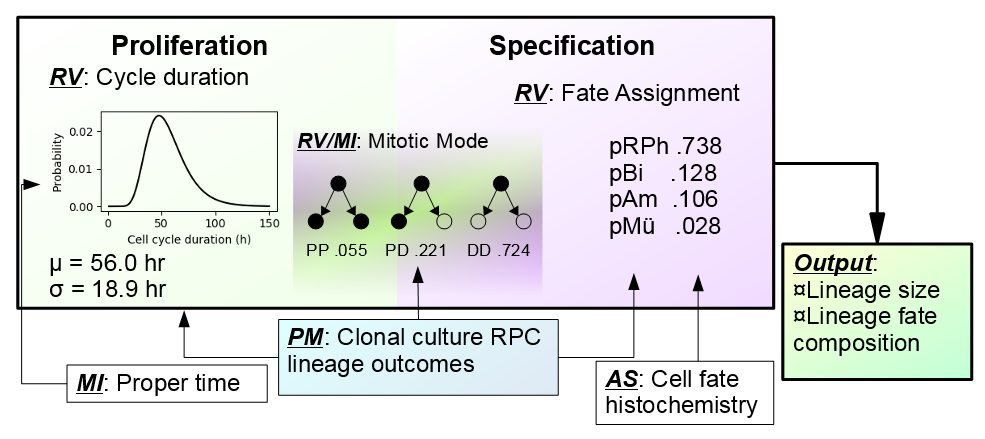
\includegraphics[width=1.2\textwidth]{ssm/Fig_1_Gomes.png}}
\caption{{\bf Structure of Gomes SSM}}
Structure of the Gomes SSM \cite{Gomes2011}. pRPh, probability of rod photoreceptor specification. pBi, probability of bipolar cell specification. pAm, probability of amacrine cell specification. pM{\"u}, probability of M{\"u}ller glia specification.
\label{GomesSSM}
\end{figure}
 
This SSM is explicitly built as a null hypothesis, or a model of background noise. It represents an extreme case in which all of the specificative and proliferative behaviours of an RPC are totally independent of all other RPCs and events in its clonal lineage. The stated purpose of this model is ``to calibrate the data", serving ``as a benchmark" \cite{Gomes2011}, a purely hypothetical apparatus to produce sequences of causally unrelated lineage outcomes. Substantial deviations of the observed data from the fully independent events of the SSM may then be interpreted as causal dependencies between RPC outcome and their relative lineage relationships, as might be observed in a developmental ``program" or algorithmic process. Finding that, with some exceptions, observed proliferative and specificative outcomes generally fall within the plausible range of Gomes SSM output, Gomes et al. conclude that RPC lineage outcomes in late embryonic rat RPCs seem to be dominated by causally independent events, suggesting that causally isolated ``noisy" macromolecular processes may give rise to the unpredictable variability in the fate outcomes of these cells. 
 
 \subsection{He SSM: Explaining variability in zebrafish neural retina lineage size}
 
The He SSM, shown in Fig \ref{HeSSM}, is deployed in a explanatory role rhetorically identical to the Gomes SSM. The extent to which model output ``captures.. aspects of the data" is taken to obviate the need for explicit ``causative hypothes[e]s". On this account, only residual error between model output and observations may be ascribed to non-stochastic processes like ``histogene[tic ordering] of cell types or a signature of early fate specification". That is, if the model can be fit to observations, this is taken to exclude the presence of any cell-autonomous temporal program, asymmetric segregation of fate determinants, extracellular influences, and the like. 

  % Place figure captions after the first paragraph in which they are cited.
\begin{figure}[!h]
\makebox[\textwidth][c]{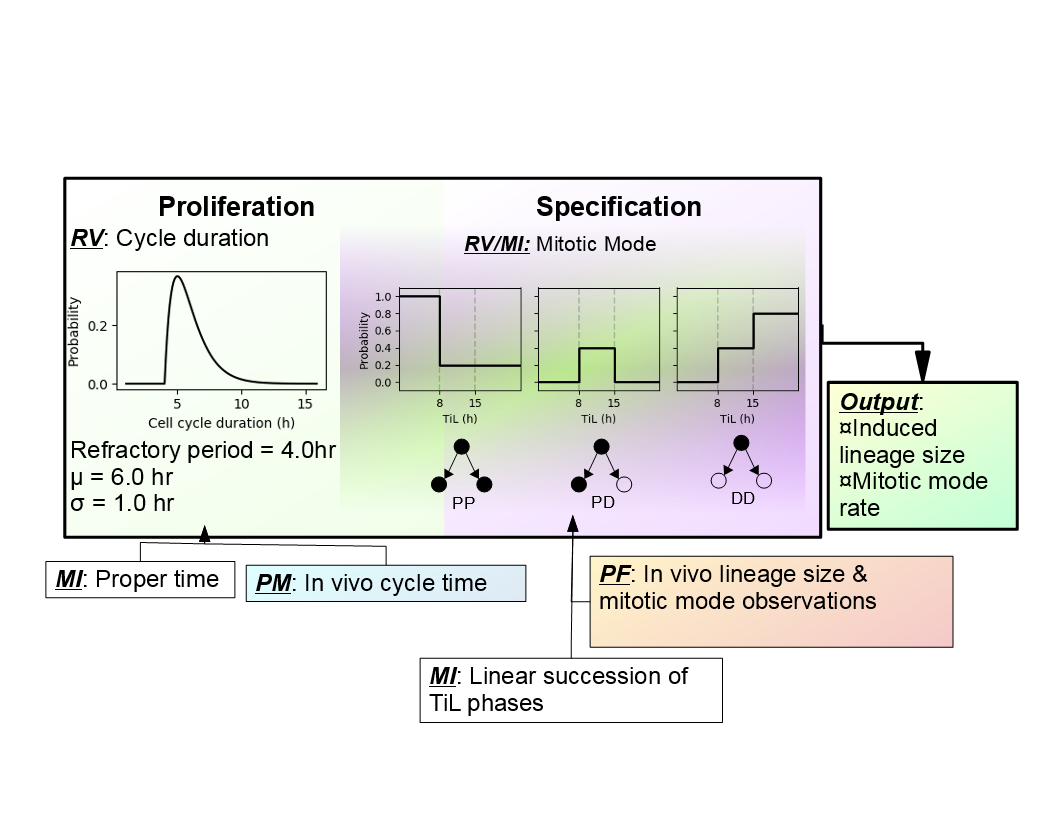
\includegraphics[width=1.2\textwidth]{ssm/Fig_2_He.png}}    
\caption{{\bf Structure of He SSM}}
Structure of the He SSM \cite{He2012}. TiL, Time in Lineage.
\label{HeSSM}
\end{figure}

There are fewer direct empirical inputs to the He model's parameters than the Gomes SSM, limited to the duration of the cell cycle. The close synchrony of zebrafish RPC divisions is modelled by assigning sister RPCs the same cycle length, shifted by a normal distribution with a variance of one hour, in contrast to Gomes RPCs, which are treated as fully independent. The lineage outcomes the He SSM is called on to explain differ significantly from those referred to by the Gomes SSM. Most notably, the Gomes SSM does not account for the early appearance of RGCs, which are not produced by the late E20 progenitors examined in that study. The zebrafish RPC lineages studied by He et al. produce all of the retinal neural types, including RGCs, which are typically produced by PD-type divisions. The He SSM does not model particular cell fates, supposing that mitotic mode is ``decoupled" from fate specification. The mitotic mode RV linking cell cycle to fate specification in the Gomes SSM has thus subsumed the specification outcomes of RPC lineages entirely, and the model is concerned only to explain the sizes of lineages (marked by an inducible genetic marker at various times), and the observed progression of mitotic modes in these early RPCs.

The He model is, therefore, called on to explain the temporal structure of the proliferative behaviour of early zebrafish RPCs that dissociated late rat RPCs do not exhibit. A Gomes-type SSM, in which the RVs determining RPC behaviour are independent of any measure of time, cannot account for this temporal progression. In order to address this, He et al., assume a linear progression of three phases which cells in each lineage pass through, the timing of these phases being determined relative to the first division of the RPC lineage, called here ``Time in Lineage" or TiL. The parameters of the mitotic mode RV are determined by these TiL phases. The temporal structure of the phases and their effect on the mitotic mode RV are selected to produce a model fit. While He et al. acknowledge that the model therefore represents a ``combination of stochastic and programmatic decisions taken by a population of equipotent RPCs," no test is performed to determine the relative contribution of the model's stochastic vs. linear programmatic elements. Instead, the purportedly stochastic nature of mitotic mode determination is emphasized throughout the report.

 \subsection{Boije SSM: Explaining variability in zebrafish RPC fate outcomes}
 
The second SMME model advanced to explain zebrafish RPC behaviour, the Boije SSM, is diplayed in Fig \ref{BoijeSSM}. This model is primarily concerned with the lineage fate outcomes that the He SSM does not treat, while abandoning the explicit proper time of the He and Gomes SSMs in favour of abstract generation-counting. The mitotic mode model-ingredient now subsumes all RPC behaviours. Boije et al. make a laudable effort to specify the particular macromolecules ostensibly involved in determining mitotic mode, nominating the transcription factors (TFs) Atoh7, known to be involved in RGC specification, and Ptf1a, known to be involved in the specification of amacrine and horizontal cells, as primary candidates. The contribution of vsx2 is taken to determine the balance between PP and DD divisions late in the lineage, with the latter resulting in the specification of bipolar or photoreceptor cells. The binary presence or absence of these signals is determined by independent RVs structured by the phase structure present in the He SSM, translated into generational time from proper time.

\begin{figure}[!h]
\makebox[\textwidth][c]{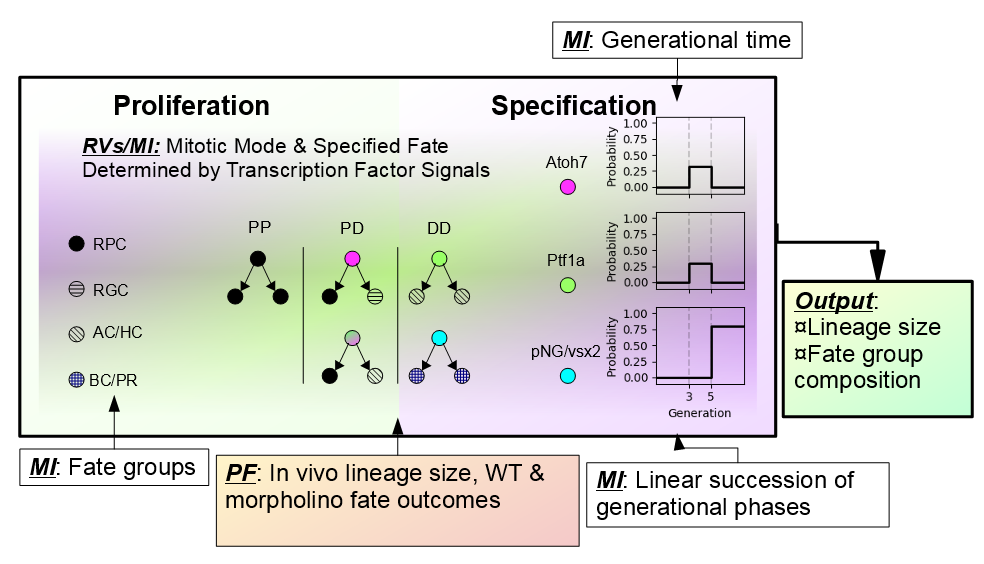
\includegraphics[width=1.2\textwidth]{ssm/Fig_3_Boije.png}}
\caption{{\bf Structure of Boije SSM}}
Structure of the Boije SSM \cite{Boije2015}. RPC, retinal progenitor cell. RGC, retinal ganglion cell. AC, amacrine cell. HC, horizontal cell. BC, bipolar cell. PR, photoreceptor. pNG- parameter representing contributions of Vsx1 and Vsx2 to specification of BC \& PR fates in absence of Atoh7 or Ptf1a signals.
\label{BoijeSSM}
\end{figure}

By this point, the SMME has become a very different type of explanation from its Gomes SSM forebear. We are no longer dealing with RVs that model causally and temporally independent processes for different aspects of RPC behaviour. There is, rather, one temporally dependent process, the determination of mitotic mode, which is explained by unpredictable subsets of each lineage generation expressing particular TF signals. Where the Gomes SSM takes its parameters directly from empirical measurements of lineage outcomes, asking whether it is sufficient to assume that these are independently determined, the Boije SSM's parameters are derived solely from model fit considerations. In spite of these considerable differences, the explanatory role of the SSM is effectively the same: the model's fit to observations is taken as evidence of the predominant influence of stochastic processes determining mitotic mode on RPC behaviour. While Boije et al. acknowledge that whether some process is called ``deterministic" or ``stochastic" is ``a matter of the level of description" \cite{Boije2015} (i.e. is a property of the model-description and not of the physical process), the explanatory role of stochasticity for RPC lineage outcomes is emphasized throughout.
 
 \subsection{Model selection demonstrates the SMME is not the best available explanation for RPC lineage outcomes}
 
From a modeller's perspective, it is notable that neither of the reports which use the He SSM \cite{He2012,Wan2016}, nor that using the Boije SSM \cite{Boije2015} report in any detail their fitting procedures, nor do any of the above report any statistical measures of goodness-of-fit. Additionally, no models representing the alternative ``theoretical options" available to explain variability in RPC lineage outcomes are compared to those advanced as evidence for stochastic processes. Given that the He SSM and Boije SSM depart from the Gomes SSM by the addition of an unexplained temporal structure to the mitotic mode model ingredient, it is striking that the overall argument remains similar to Gomes et al.'s, despite the persuasive force of the latter deriving from the lack of such structures. While He et al. and Boije et al. acknowledge that their models involve both stochastic and linear programmatic elements, their relative influence on model output is not measured, and macromolecular explanation is only applied to the stochastic elements. Moreover, the emphasis on this mitotic mode model construct increases with each successive model, to the extent that in the Boije model there are no other elements that are used to explain RPC behaviours. All cellular behaviours are, in effect, progressively collapsed into the stochastic mitotic mode concept. Finally, the He and Boije SSMs contain more parameters, which are determined by fewer empirical measurements than the Gomes SSM. It is therefore important to test whether the most important ingredient in these models is the stochastic mitotic mode, against the possibility the unexplained temporal structure is the truly explanatory element.

Fortunately, we may employ model optimisation and selection techniques to adjudicate this. The most straightforward way to do so is to reexamine the He SSM alongside a competing alternative model. The data to which the He SSM has been applied is amenable to a scheme in which the models are fit to a ``training" dataset, followed by a ``test" dataset. In this case, the training data are the induced lineage size and mitotic mode rate data from He et al. The test dataset comprises the Atoh7 morpholino observations from He et al., and the CMZ lineage size data from Wan et al. This allows us to test how well the He SSM, and an alternative, hold up under novel experimental conditions, without relying on a trivial ordering of goodness-of-fit to training data. Since the Boije SSM draws straightforwardly on the He SSM for its temporal phase-parameterisation and stochastic mitotic mode model ingredient, this analysis of the He SSM also bears directly on the validity of the Boije SSM.

As an alternative to the SMME He SSM, we constructed a model that has a deterministic mitotic mode with variable phase lengths. Rather than variability arising from a stochastic-process mitotic mode changing across phases of fixed length, we simply supposed that mitotic mode is deterministic in each phase (guaranteed PP mitoses in the first phase, PD in the second, and DD in the third), but the phase lengths are variable between lineages and shift slightly between sister cells. That is, we represented this linear progression of deterministic mitotic mode phases using the same type of statistical construct the He SSM applies to model cell cycle length, to avoid introducing any novel or contentious elements into the model comparison. More specifically, each lineage has a first PP phase length drawn from a shifted gamma distribution, followed by a second phase length drawn from a standard gamma distribution. Upon mitosis, these phase lengths are shifted in sister cells by a normally distributed time period, exactly like cell cycle lengths in the He SSM.

We take this to be a reasonable representation of the classic suggestion that RPCs step through linear succession of competency phases, given the conceptual tools that the He SSM uses to model mitotic phenomena. If we suppose that this temporal program is governed by RPC lineages passing through a stereotypical series of chromatin configurations which allow for PP, then PD, then DD mitoses in turn, along with the associated competence to produce the particular cell fates associated with PD and DD mitoses, it seems entirely plausible to suggest that lineages differ in the lengths of time they occupy each state. This is particularly true if we concede that an SSM, foregoing any spatial modelling whatsoever, must necessarily abstract extracellular and spatial influences on these processes. Moreover, since these chromatin configurations must be broken down and rebuilt with each mitosis, the re-use of the ``sister shift" model ingredient from the He SSM's cell cycle RV is congenial, representing the same sort of cell-to-cell variability that results in the small differences between sister cells in cycle timing. 

While the code used to implement the SSMs mentioned above has not been published, the relevant reports provide enough detail to reconstruct these models in full, which we did using the CHASTE cell-based simulation framework, in order to provide transparent and reproducible implementations of the SSMs. Because the values selected for the He SSMs' parameters seem to have been selected as a series of rough estimates, with only the value for the probability of PD-type mitoses in the second model phase being varied to produce the fit, we suspected that the fit would not be at or near the local minimum for a loss function. That is, a model fit produced in this manner is likely to be located in a region of the parameter space that is highly sensitive to small perturbations, and therefore may depend strongly on implementation-specific idiosyncracies. He et al. report that they experienced difficulty in obtaining a good fit to their 32 hour induction data, with changes in the phase two PD probability producing large differences in fit quality. Unsurprisingly, when we rebuilt the He SSM with the original fit parameterisation, we substantially reproduced the original fit, except for the 32 hour data, where the model output diverges substantially from that reported in He et al. (see \nameref{originalSupplement}). Since this is clearly not the best fit available for the He SSM, and we wish to directly compare the best fits (i.e. the parameterisations at minima of some loss function) for the He SSM and our putative alternative model, we used the simultaneous perturbation stochastic approximation (SPSA) algorithm \cite{Spall1998} to optimise both models against test data. SPSA is particularly convenient for complex, multi-phase models like the He SSM, because no knowledge of the relationship between the model's parameters and the loss function is required. We used Akiake's information criterion (AIC) as the loss function to be minimised, in order to provide a rigorous comparison between the two differently-parameterised models (the deterministic alternative has two fewer parameters than the He SSM). 

\begin{figure}[p]
	\makebox[\textwidth][c]{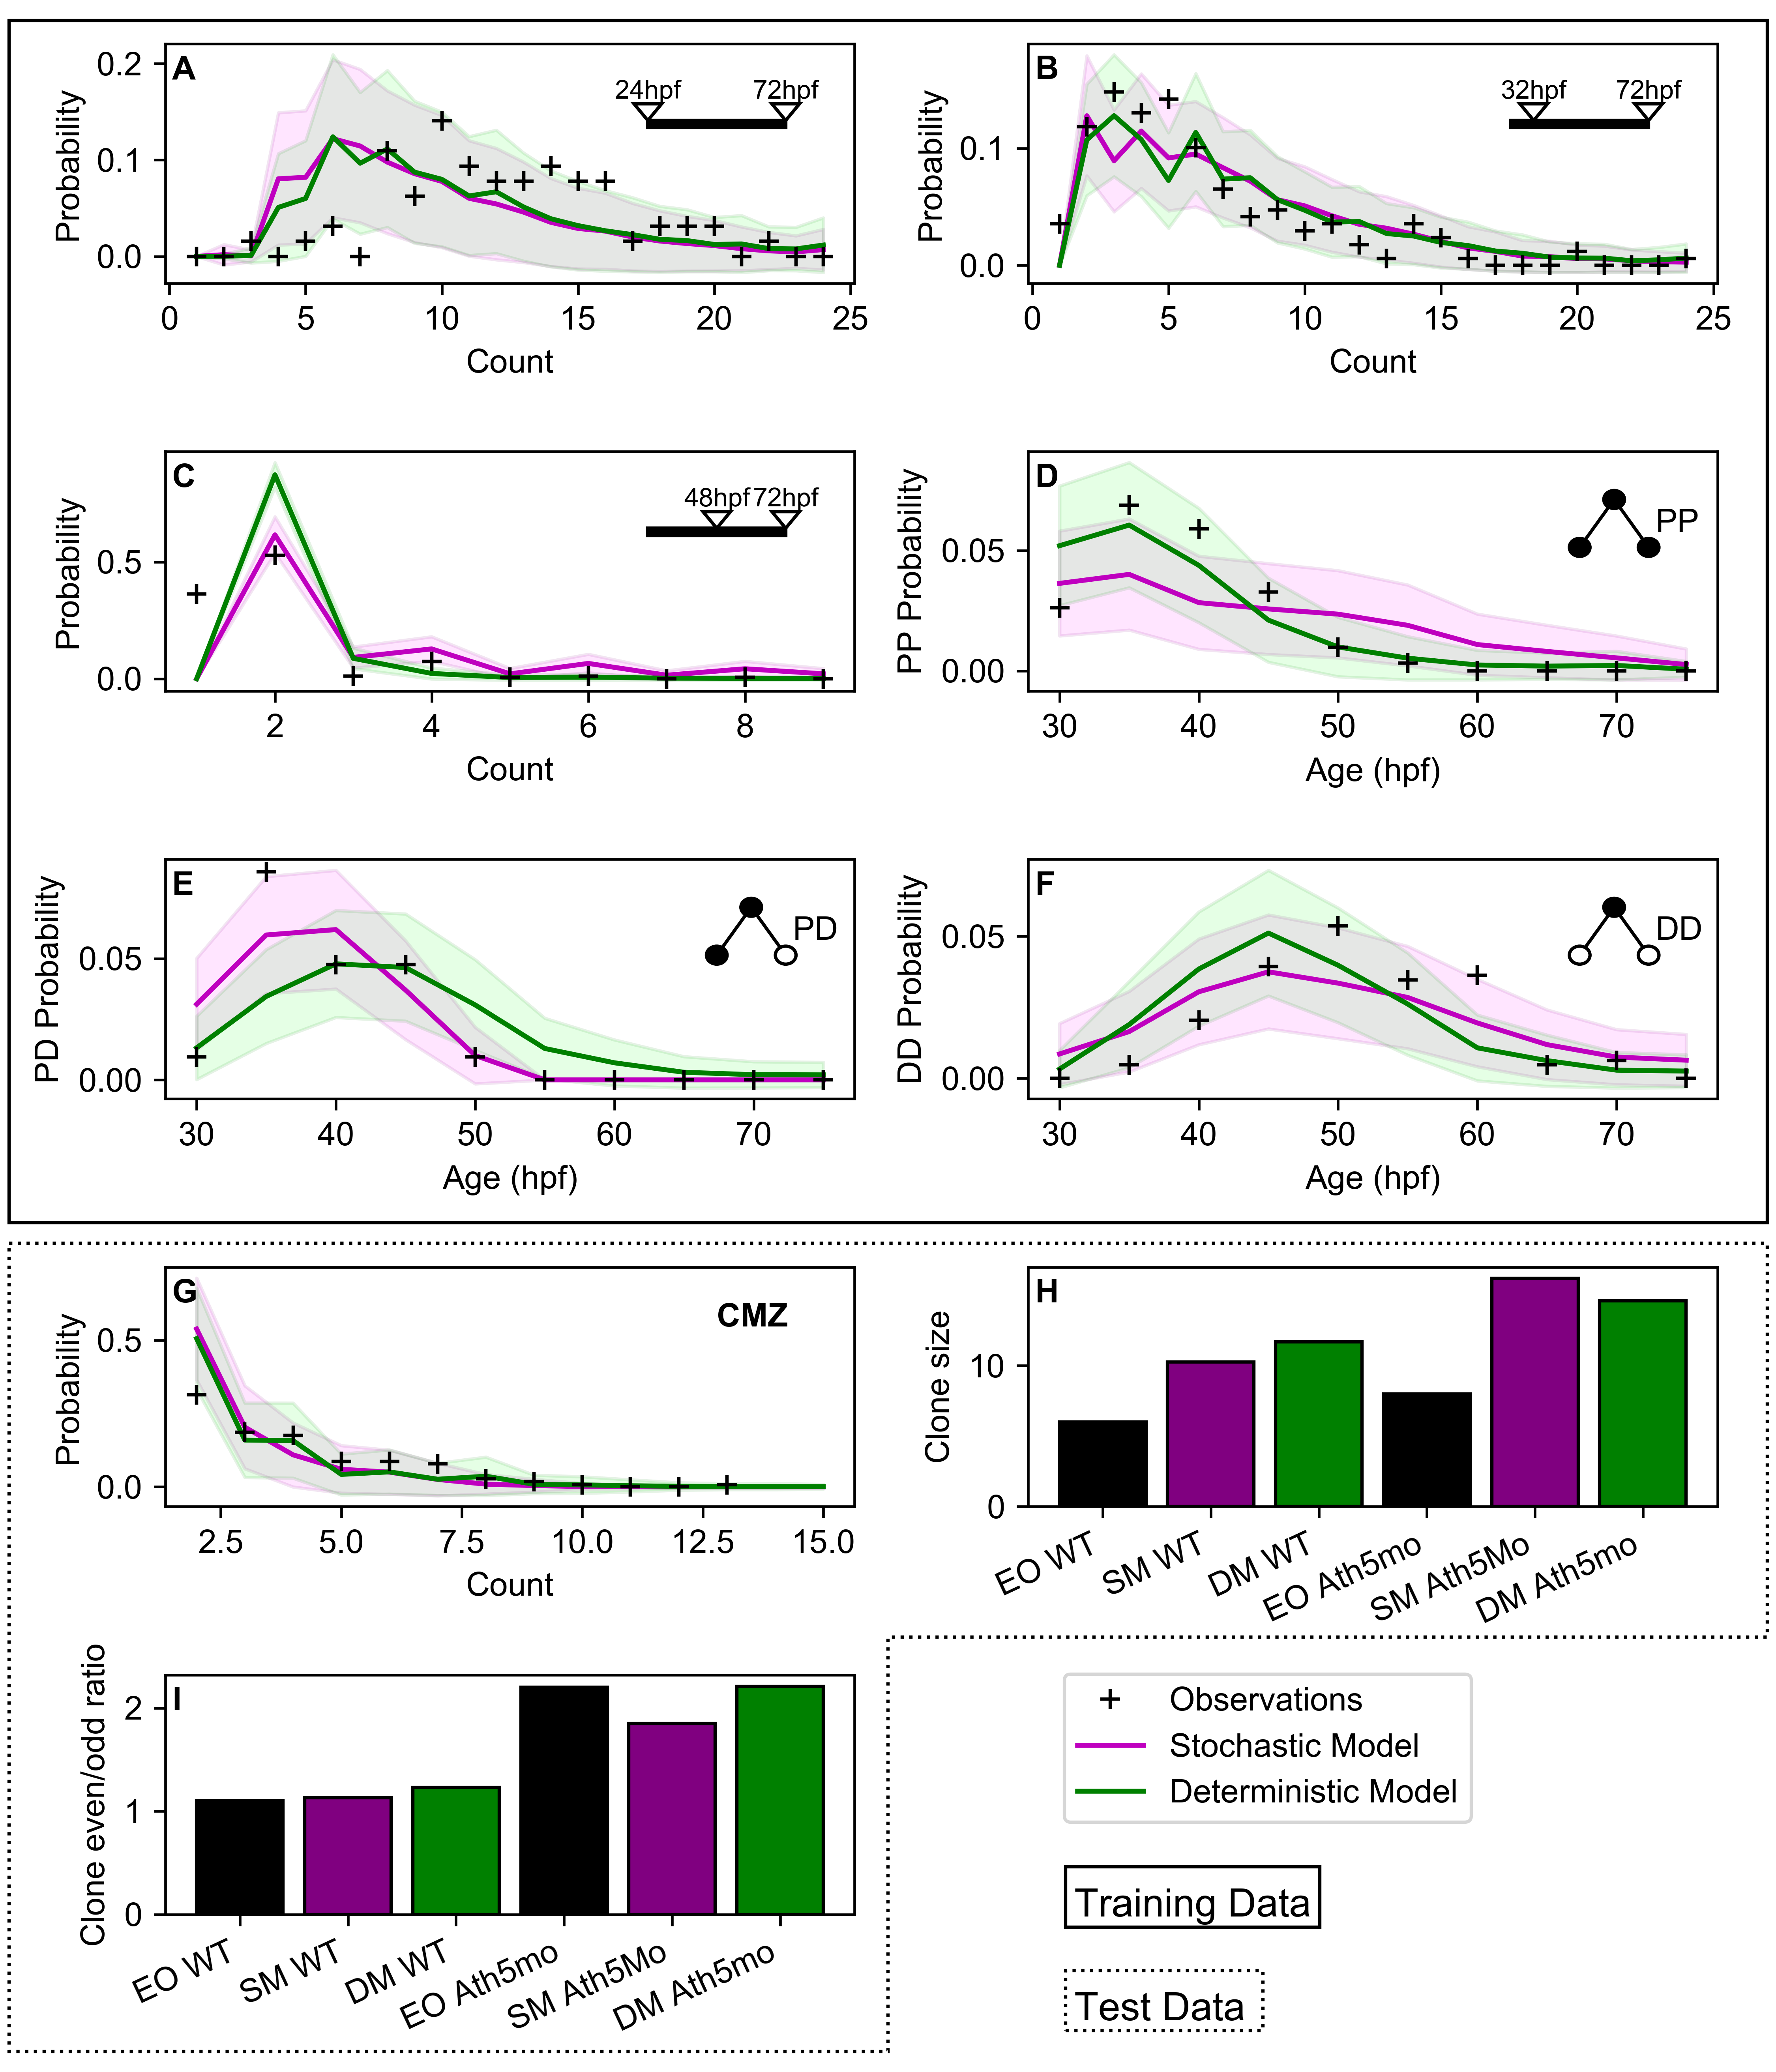
\includegraphics[width=1.\textwidth]{ssm/Fig_4_model_comparison.png}}
\caption{{\bf Model comparison: the SPSA-optimised He SSM and a deterministic alternative}}
Empirical observations (black crosses and bars) and SPSA-optimised model output (magenta, stochastic mitotic mode model; green, deterministic mitotic mode model). Model output in panels A-G is displayed as mean $\pm$ 95\% CI. Panels A-F: Training dataset, to which models were fit. Panels A-C: Probability of observing lineages of a particular size ("count") after inducing single RPC lineage founders at (A) 24, (B) 32, and (C) 48 hours with an indelible genetic marker, tallying their size at 72hpf. Panels D-F: Probability density of mitotic events of modes (D) PP, (E) PD, and (F) DD over the period of retinal development observed by He et al. Panel G: Probability of observing lineages of a particular size ("count") originating from the CMZ; RPCs are taken to be resident in the CMZ for 17 hours before being forced to differentiate, lineage founders are assumed to be evenly distributed in age across this 17 hour time period. Panel H: Average clonal lineage size of wild type and Ath5 morpholino-treated RPCs. Ath5mo treatment is taken to convert 80\% of PD divisions, which occur in the second phase of the He model, to PP divisions, resulting in larger lineages. Panel I: Ratio of even to odd sized clones in wild type and Ath5 morpholino-treated RPCs.
Methods in \autoref{ssec:CHASTEsims}.
Code in \autoref{ssec:He_output_plot}.
\label{SDFig}
\end{figure}
\FloatBarrier

After fitting to the training dataset, we calculated AIC for the He SSM (hereafter SM, for stochastic model) and our deterministic mitotic mode alternative (hereafter DM), for both training and test datasets. The combined results are displayed in Fig \ref{SDFig}, with the output of the two models being presented separately in \nameref{stochasticSupplement} and \nameref{deterministicSupplement}. Remarkably, the DM closely recapitulates the output of the SM for both datasets. Moreover, while the more highly-parameterised SM permits a better fit to the training data, the DM proves to be a better fit to the test dataset, as summarised in Table \ref{AICtable}. This can be understood as a case of model overfitting: a higher-parameter model fits some training dataset better than a simpler model, but fails upon challenge with a new dataset. Given this model selection scheme, it is plain that we should choose the DM over the SM as a superior explanatory model, both on the basis of explanatory power and of Occam's Razor.

\begin{table}[!ht]
\centering
\caption{
{\bf AIC values for models assessed against training and test datasets}}
\begin{tabular}{|l|l|l|}
\hline
{\bf Model} & {\bf Training AIC} & {\bf Test AIC} \\ \hline
Stochastic (He fit) & -93.26 & 255.64\\ \hline
Stochastic (SPSA fit) & {\bf -93.80} & 92.24\\ \hline
Deterministic (SPSA fit) & -69.33 & {\bf 86.60}\\ \hline
\end{tabular}
\begin{flushleft} AIC: Akiake's information criterion. Lower values reflect better model explanations of the noted dataset. Lowest values are noted in bold.
Methods in \autoref{ssec:CHASTEsims}.
Code in \autoref{ssec:He_output_plot}.
\end{flushleft}
\label{AICtable}
\end{table}

We therefore conclude that the SMME is not the best available explanation for variability in zebrafish RPC lineage outcomes. It is clear from this analysis that the assumed, but unexplained, linear succession of mitotic mode phases is what provides the overall structure of the model output. Variability in lineage outcomes may be supplied by entirely different model ingredients without any loss of explanatory power on new datasets (indeed, with some improvement, in our case). To conclude that these models support a stochastic process governing mitotic mode, ruling out other types of explanation, is unjustified. It is likely that any number of different types of SSMs, representing other sorts of processes (such as asymmetric segregation of fate determinants, or differential spatial exposure to extracellular signals), can produce identical model output. Given this, we conclude that SSM models of this type are inadequate for the task of locating the source of variability in RPC lineage outcomes.

\subsection{SMME SSMs cannot explain the post-embryonic phase of CMZ-driven zebrafish retinal formation}

The zebrafish retina, like other fish retinas, and unlike the mammalian retina, continues to grow long after the early developmental period, indeed, well past the organism's sexual maturity. This may be unsurprising, given that zebrafish increase in length almost ten-fold over the first year of life \cite{Parichy2009}, necessitating a continuously growing retina during this period. In fact, the quantitative majority of zebrafish retinal growth occurs post-metamorphosis, outside of the early developmental period. This growth occurs due to the persistence of a population of proliferative RPCs present in an annulus at the periphery of the retina, called the ciliary or circumferential marginal zone (CMZ), which plates out the retina in annular cohorts. A typical "tree-ring" analysis from our studies, marking the DNA of cohorts of cells contributed to the retina at particular times with indelible thymidine analogues, is shown in Fig \ref{RingFig}. These experiments show the structure of the adult zebrafish retina is quantitatively dominated by contributions from the CMZ in the period between one and three months of age. Why peripheral RPCs in zebrafish remain proliferative, while those in mammals are quiescent \cite{Tropepe2000}, and whether and how their behaviour might differ from embryonic RPCs, remain unresolved. Answers to these questions may have significant fundamental and therapeutic implications, especially given e.g. the possibility of harnessing endogenous, quiescent, peripheral RPCs in humans for regenerative retinal medicine.

\begin{figure}[!h]
\makebox[\textwidth][c]{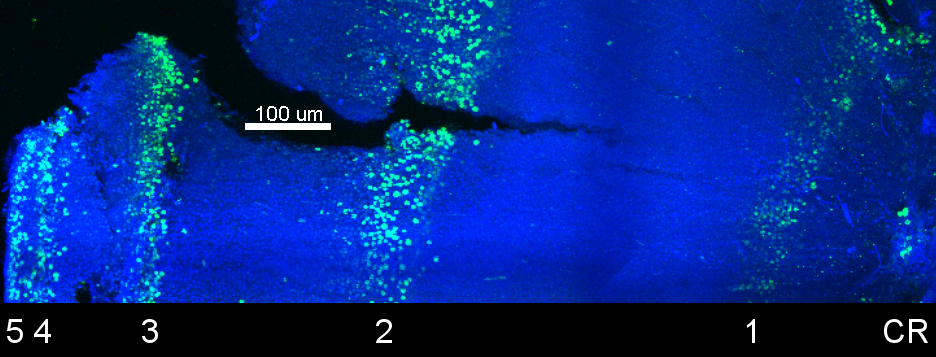
\includegraphics[width=1.\textwidth]{ssm/Fig_5_CMZ_cohorts.png}}
\caption{{\bf Most zebrafish retinal neurons are contributed by the CMZ between one and three months of age}}
Maximum intensity projection derived from confocal micrographs of a zebrafish whole retina dissected at 5 months post fertilisation (mpf). The animal was treated with BrdU at 1, 2, 3, 4, and 5 mpf for 24hr. Anti-BrdU staining of the whole retina reveals the extent to which the CMZ (which is responsible for retinal growth after approximately 72hpf) contributes new neurons in tree-ring fashion, extending out from the center of the retina (CR), which is formed before 72hpf. Monthly cohorts are labelled appropriately. Scale bar, 100 $\mu$m.
Methods in \autoref{ssec:SMMEwholeretina}.
\label{RingFig}
\end{figure}

\FloatBarrier

The He SSM was deployed in Wan et al. \cite{Wan2016}, with the claim that the He SSM explains the behaviour of CMZ RPCs. Wan et al. argue that a slowly mitosing population of bona fide stem cells, at the utmost retinal periphery, divides asymmetrically to populate the CMZ with He-SSM-governed RPCs. In other words, the usual suggestion that CMZ RPCs undergo a somewhat different process than embryonic RPCs, perhaps recapitulating across the peripheral-central axis some progression of states or lineage phases that embryonic RPCs pass through in time \cite{Harris1998}, is repudiated in favour of one model which describes the behaviour of all RPCs throughout the life of the organism, with the addition of a small population of stem cells to keep the CMZ stocked with RPCs. If so, this might suggest that the problem of activating quiescent stem cells in the retina is simply that- one need only sort out how to throw the proliferative switch in these cells, since the proliferative and fate specification behaviours of the resultant RPCs will reliably be the same as those observed in development.

While we determined that the SMME is not the best available explanation for RPC lineage outcomes, we still felt that the SSMs associated with this explanation might be used to elucidate this point. In particular, if it is the case that the He SSM provides good estimates of lineage size and proliferative dynamics in the early zebrafish retina, it should be possible, using this model, and the estimates of putative stem cell proliferative behaviour provided by Wan et al., to simulate the population dynamics of the CMZ, at least through the first few weeks of the organism's life.

In pursuing this point, we noted a peculiar feature of the He SSM not documented by any of the SMME reports: the cell cycle model overstates the  \textit{per-lineage} rate of mitoses by as much as a factor of 3. That is, the mitotic mode rate data presented in He et al., recapitulated here in Fig \ref{SDFig}, panels D, E, and F, and used to optimise both the SM and DM, are probability density functions that are not standardised on a per-lineage basis. These data simply indicate the distribution of mitotic events of a particular type. When we take all of the mitotic events documented by He et al. and calculate the probability of any such event occuring per lineage, per hour, we obtain the values presented in Fig \ref{PerLineageFig}.

\begin{figure}[!h]
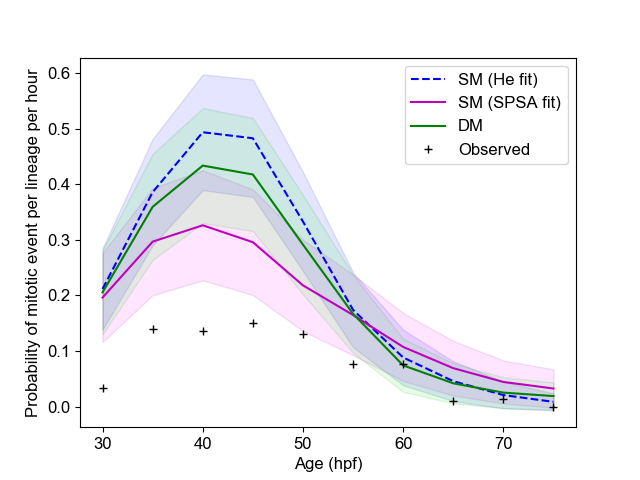
\includegraphics{ssm/Fig_6_per_lineage_mitotic_rate.png}
\caption{{\bf Per-lineage probabilities of mitoses, He et al. observations compared to model output}}
Probability of observing a mitotic event over the period studied by He et al., per hour, per lineage. Model output is presented as mean $\pm$ 95\% CI.
Methods in \autoref{ssec:CHASTEsims}.
Code in \autoref{ssec:Mitotic_rate_plot}.
\label{PerLineageFig}
\end{figure}

Similarly, when we performed cumulative thymidine analogue labelling of the 3dpf CMZ, (using the assumptions of Nowakowski et al. \cite{Nowakowski1989}, which treat the proliferating population as a homogenous, and dividing asymmetrically; these assumptions are flawed but adequate for a rough estimate) we obtain an average cell cycle length of approximately 15 hours, more than twice as long as the He SSM's mean cycle length. These data are displayed in \ref{cumulativeSupplement}. Therefore, the He SSM (in both its original and refit parameterisation, as well as the deterministic alternative, since they all rely on the same proliferative model elements) substantially overstates the proliferative potential of both embryonic and early CMZ RPCs. Since we observed a massive build-up of proliferating RPCs between two and four weeks post-fertilisation, we thought this might actually suit this later context better.

To estimate of total annular CMZ population in zebrafish retinas over time, we counted proliferating RPCs present in central coronal sections of zebrafish retinas throughout the first year of life, treating these as samples of the annulus, and calculated the total number of cells that would be present given the diameter of the spherical lens measured at these times. Our simulated CMZ populations were constructed at 3dpf by drawing an initial population of RPCs governed by the He SSM (using the original fit parameters, which further exaggerate the proliferative potential of these lineages) from the observed distribution. We added immortal stem cells amounting to one tenth of this total. This is likely an overestimate, given that these putative stem cells are thought to be those in the very peripheral ring of cells around the lens, of which typically two to four may be observed in our central sections with an average of over one hundred proliferating RPCs. Moreover, these simulated stem cells were given a mean cycle time of 30 hours, proliferating about twice as quickly as Wan et al. suggest. Finally, to reflect the fact that these stem cells contribute to the retina in linear cohorts \cite{Centanin2014}, and more of them are therefore required as the retina grows, the stem cells were permitted to divide symmetrically when necessary to maintain the same density of stem cells around the annulus of the lens. Two hundred such CMZ populations were simulated across one year of retinal growth.

The results of these simulations are displayed in Fig \ref{WanSim}, overlaid over CMZ population estimates derived from observations. Given the generous parameters of the population model, consistently overestimating the proliferative potential of embryonic and early CMZ RPCs, it is surprising that the He SSM proves completely unable to keep up with the growth of the CMZ in the first two months of life. Indeed, the unrealistically active stem cell population the simulated CMZs are provided with is unable to prevent a near-term collapse in RPC numbers, only catching up after the months later as the number of stem cells increases with the growth of the lens. Thus, even given permissive model parameters, the He SSM is not able to recapitulate the quantitatively most important period of retinal growth in the zebrafish.

\begin{figure}[!h]
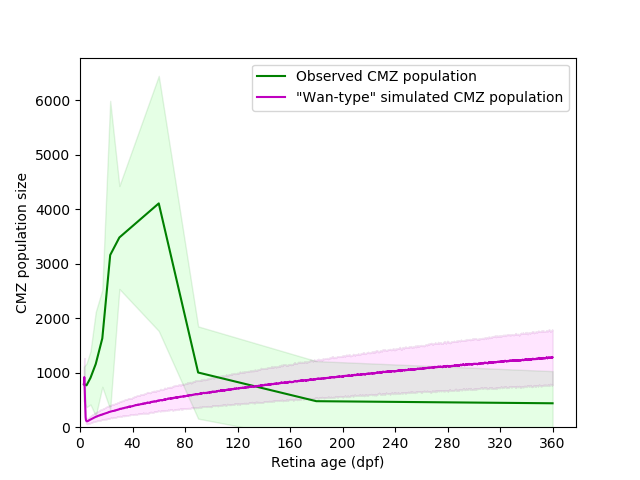
\includegraphics{ssm/Fig_7_wan.png}   
\caption{{\bf CMZ population of proliferating RPCs: estimates from observations and simulated Wan-type CMZs}}
Annular CMZ population was estimated from empirical observations of central coronal cryosections stained with anti-PCNA, a marker of proliferating cells, standardising by the diameter of the spherical lens observed in these animals. "Wan-type" CMZs were initialised with a number of RPCs drawn from from the observed 3dpf population distribution, and given an additional 1/10\textsuperscript{th} of this number of immortal, asymmetrically dividing stem cells, as described in the text, and simulated for the first year of life. All data is presented as mean $\pm$ 95\% CI.
Methods in \autoref{ssec:PCNA}, \autoref{ssec:CHASTEsims}.
Code in \autoref{ssec:Wan_output_plot}.
\label{WanSim}
\end{figure}

This analysis suggests that observations of RPCs in embryogenesis and early larval development are unlikely to provide a good quantitative model of the development of the zebrafish retina, even abstracting away spatial and extracellular factors as SSMs necessarily do. Our data point to a second, quantitatively more important phase of retinal development, between approximately one and four months of age, in which RPCs are far more proliferatively active than in early development. It is likely that models that closely associate proliferative behaviour with fate specification, like those of the SMME, will be unable to explain this period. Recent evidence suggests that mitotic and fate specification behaviours in RPCs may be substantially uncoupled \cite{Engerer2017}. This would permit the CMZ population to scale appropriately with the growing retina. Alternatively, it is possible that RPCs have heterogenous proliferative behaviour, and that this heterogeneity is mainly apparent later in development.

\section{Conclusion}

Simple stochastic models are familiar tools for stem cell biologists. Introduced by Till, McCulloch, and Siminovitch in 1964 \cite{Till1964}, they proved their utility in describing variability in clonal lineage outcomes of putative stem cells, originating from macromolecular processes beyond the scope of cellular models (and beyond the reach of the molecular techniques of the time). More prosaically, their simplicity afforded computational tractability in an era when processing time was relatively scarce, allowing early access to Monte Carlo simulation techniques. That said, their abstract nature emphasizes an aspatial, lineage-centric view of tissue development, which cannot account for the generation of structurally complex tissues like retinas beyond cell numbers, and, perhaps, fate composition. As a result of this relatively loose relationship to the complex morphogenetic environment, there are few constraints on the model configurations that may produce similar outputs. This can result in modellers being led astray by their apparently good fits to observations, which is why the fit of one highly parameterised model cannot be taken, alone, as evidence for some theory; it is very rare that there is not a model representing an alternative theory that cannot be made to produce a reasonable model fit. Indeed, as we demonstrate here, the use of standard model selection techniques may make plain that a completely contradictory theory is a better explanation for the data.

To some extent, this can be ameliorated by careful attention to the particular macromolecular or cellular referents that particular model constructs represent. The ``mitotic mode" construct present in all SSMs is a particularly ambiguous and problematic one in this regard. ``Mitotic mode" is not, itself, a property of a mitotic event, but is rather a retrospective classification of the event after an experimenter observes whether progeny resulting from the event continue to proliferate. Its original appearance in SSMs was simply to allow calculation of clonal population sizes; it was never intended to represent a particular type of process or ``decision" made by cells at the time of mitosis to continue proliferating or not. Any number of pre- or post-mitotic signals and processes may result in a particular mitosis being classified as PP, PD, or DD, without anything about the mitotic event itself determining this. The use of such a retrospective classification, rather than the identification of some physical property of the mitotic event (such as the asymmetric inheritance of fate determinants), is straightforwardly a concession that the actual macromolecular determinants of cellular fate are outside the scope of the model.

The SMME represents an attempt to connect this abstract, retrospective model construct to observations of noisy gene transcription \cite{Raj2008}. Motivated by the observation that momentary mRNA transcript expression in RPCs is highly variable from cell-to-cell \cite{Trimarchi2008}, the suggestion is that this transcriptional noise may be responsible for the observed variability in RPC lineage outcomes. Since this noise may be ``tuned" to a degree by e.g. promoter sequences \cite{Raser2004}, it could plausibly be under selective pressure. There are two significant problems with identifying the SMME's stochastic mitotic mode with this type of process. The first we have demonstrated by constructing an alternative model with deterministic mitotic mode but variable phase lengths: the source of variability may be located elsewhere without compromising the explanatory power of the model. It is therefore impossible to determine what sort of process might give rise to variability in RPC lineage outcomes by using SSMs in this fashion. The second, more fundamental problem is that a causal explanation of the presence of the signal, for which noise is a property, is elided entirely in favour of emphasis on ``stochasticity". This is most apparent in the Boije SSM. In this model, Atoh7 and Ptf1a TFs are available to provide their noisy signal in the 4th and 5th lineage generations, and at no other time. We do not dispute that a noisy signal may contribute to variability in that signals' effects; rather, we suggest that it is the temporal structure of such a signal (assuming this structure can be empirically demonstrated, rather than assumed) that calls for causal explanation. The SMME reports explicitly disclaim the necessity for ``causative hypotheses" in the case that a stochastic model provides a good fit to observations. As Jaynes remarked in his classic text on probability theory, ``[stochasticity] is always presented in verbiage that implies one is describing an objectively true property of a real physical process. To one who believes such a thing literally, there could be no motivation to investigate the causes more deeply ... and so the real processes at work might never be discovered." \cite{Jaynes2003} 

In identifying the model construct with the physical processes determining RPC outcomes, the SMME obscures what seems to us to be the primary lesson to be drawn from the Harris groups' beautiful in vivo studies of zebrafish RPCs. That is, compared to late rat RPCs in dissociated clonal culture, RPCs in intact zebrafish retinas produce far more orderly outcomes. To the extent that these outcomes are variable, the source of variability remains unidentified. We suggest that resort to ``stochasticity" as an explanatory element should not be made in the absence of model comparisons that rule out alternatives with well-defined causal structures, lest we fall into the trap Jaynes warned us about.
\chapter{Toward a computational CMZ model comparison framework}
\label{chap:SMMEoutro}
\section{SMME Postmortem: a wrong turn at Gomes}
To return to the question posed in \autoref{sec:SMMEexplanatorystrat}: has the SMME succeeded in finding order by blurring out the chaotic welter of mechanistic explanations for RPC function in retinogenesis? \autoref{chap:SMME} argues the structure of the SMME models support explanations based on the original idea of a linear, deterministic series of stages through which RPCs progress, originally put forward by Cepko et al. \cite{Cepko1996}, rather than the stochastic processes which are their rhetorical emphasis. The important feature of the SMME models is where they depart from the original Gomes SSM: the assumption of the linear structure of temporal phases. The succession of stages is the model ingredient that produces the structure resembling the data, not the various random variables associated with mitotic mode, which we have proven by demonstrating that a deterministic progression of mitotic mode models the observations better than its stochastic counterpart. By introducing variability into the lengths of the linear temporal program already assumed by the SMME models, we can remove variability from the mitotic mode and produce a superior model with fewer parameters. Only by the process of counterinduction \cite{Feyerabend1993}, the comparison of models with different propositional structures about reality, does this become clear. The introduction of the linear phase structure is required to model the early contribution of RGCs in zebrafish. If this is left without some biological rationale, retinogenesis remains unexplained. The SMME thus does not achieve its aim of being a complete description of lineage outcomes in retinogenesis, and this is confirmed by our observation that the Wan model \cite{Wan2016} has little explanatory power outside the first few days of life, which makes up a small portion of the total retinal contribution to the zebrafish retina.

We must, therefore, assess that Harris' first theoretical maneuver, explaining the data with a model whose structure supports a stochastic resolution of mitotic mode ``decisions'', fails in the face of an alternative which locates stochasticity elsewhere. The underlying data used to inform these models speak better to an entirely different selection from the array of theoretical options outlined in \autoref{sec:TheoryOptions}, the linear progression of competencies. Because the SSM model form does not usually have spatial dimensions, we did not test models involving variablility in extracellular signals, but it is a good bet that such a model could be made to fit about as well as either of the ones tested in the previous chapter. In effect, if we are to follow Harris' inferential logic, variability in RPC outcomes can be explained by ``stochastic variability" in any model parameter which affects fate outcomes. Because of the seriousness of this problem for biological inferences, an explanation of the Bayesian epistemological view of probability has been provided in \autoref{sec:BayesEpistemology}. Moreover, a thorough argument that ``stochasticity'' cannot be a property of real existents is provided in \autoref{sec:chance}. It suffices here to conclude that the SMME models do not achieve the aim of supporting ``stochastic processes'' as explanations over the alternatives.

The second theoretical maneuver was to nominate a particular macromolecular system as the physical locus of the stochastic process, in this case represented by Atoh7 and Ptf1a as labels for abstract Bernoulli distributed processes. It remains obscure in what sense the model variables relate to their namesake transcription factors (transcription of the TF itself? activation of other genes?), and no measurements of these factors inform parameter selection. Plainly, these factors are involved in relevant RPC behaviours, but it is unclear why they have been nominated as causally upstream of the ``mitotic mode'' selection. Since the Boije model inherits the assumption of a linear progression of stages, it is very likely that a model with similar explanatory power could be built using the same strategy outlined above, locating random variability outside mitotic mode, although this is outside the scope of the present work.

On the basis of the above, we can conclude that the sole formally testable model of RPC function in the zebrafish retina is not adequate for our purposes. But how did we get here? As noted in \autoref{Raff}, the notion that the most significant behaviours associated with RPCs are produced by mechanisms intrinsic to the cells derives much of its empirical support from the Raff group's work. This story began with the observation that co-culturing E15 rat RPCs in dissociated pellet cultures with P1 cells did not accelerate the appearance of the first rods derived from the E15 progenitors (which occurred at a similar time as \textit{in vivo}), suggesting a partially intrinsic commitment ``schedule" for these cells\footnote{Co-culturing with P1 cells, did, however, significantly increase the proportion of E15 RPCs specified as rods, resulting in Raff's suggestion here that both intrinsic and extrinsic factors are important.} \cite{Watanabe1990}. The scope of these observations were dramatically expanded by Raff's subsequent work, intended to address the relative significance of intrinsic versus extrinsic processes in RPC function by comparing clonal RPC lineages in fully dissociated clonal-density cell culture to those in intact explants \cite{Cayouette2003}. The remarkable finding of this study was that dissociated E16-17 rat RPC lineages produce very similar numbers and types of retinal neurons as their tissue-embedded counterparts, albeit without morphological or molecular markers of mature neurons. This observation provided strong evidence for the predominant importance of RPC-intrinsic processes in determining both mitotic and fate outcomes for late RPC lineages. The complex, spatially organised context of intact explanted tissue seemed to only be required for the maturation of neurons, and was not required to regulate proliferation or the initial commitment to an appropriate distribution of lineage outcomes. As correct cell numbers and types are the two most obvious and critical parameters that must be achieved for RPCs to produce a functional retina of the appropriate size, the suggestion that both are largely determined by intrinsic processes seemed a striking confirmation of Williams and Goldwitz's much earlier suggestion \cite{Williams1992}, against the prevailing view of the day, that lineage had a greater role to play than cellular microenvironment in RPC contributions. Interestingly, Raff's interpretation of their 2003 data was that RPCs were most likely stepping through a linear, programmed developmental sequence rather than undergoing shifts in the probabilities of variable outcomes over time. It is notable that this interpretation arises not from the data collected in their study, but from considerations of a single unusual clone reported by \cite{Turner1990}, and by analogy with drosophila neuroblasts. In retrospect, these arguments for linear sequences of deterministic RPC outcomes do not seem particularly strong, and it is perhaps unsurprising that these studies are remembered mainly for highlighting the importance of RPC-intrinsic processes.

The Gomes study, with its detailed study of particular rat late-embryonic RPC lineages, thus seemed to solidify the notion that unpredictable RPC-intrinsic processes dominate lineage outcomes \cite{Gomes2011}. But this study, like its forebears originating in Raff's work, is concerned with a population of RPCs that is too old to produce RGCs. This is the essential point: the SMME does not try to explain the early appearance of RGCs in terms of some macromolecular mechanism, although this is the single most significant difference between the zebrafish RPC lineages studied by Harris and the rat lineages studied by Raff and Cayouette \cite{Cayouette2003, Gomes2011}. It is only by assuming the unexplained linear temporal structure of RPC specification that the SMME models achieve their apparently good explanatory quality.

\section{Implications of the SMME study for modelling CMZ RPCs}
Having taken seriously the possibility that an adequate model of zebrafish retinogenesis already exists, and concluded in the negative, we may ask how to improve on this state of affairs. Firstly, lessons in statistical acumen must be learned. Careful model optimization is needed, and to have any confidence about our interpretation of the model, we must test alternatives that make fundamentally different assumptions about the causal structure of the phenomenon being explained by the models. Can we conclude that the approach used in \autoref{chap:SMME} is adequate to our task? There are two broad elements to consider here: the appropriateness of the overall modelling approach represented by the SSM in relation to the hypotheses we wish to test, as well as the soundness of the statistical procedures.

Taking up the SSM, by far its most attractive features are its computational efficiency and the ease of producing a custom model to fit some particular case-  the SMME models include some elements like the correlation of cell cycle lengths in mitotic sisters that greatly improve the temporal modelling of RPC lineage outcomes, for instance, which we will adopt in simulations presented below. The observations arising from the SMME strongly suggest that we would like to test hypotheses about RGC specification in order to find better models of RPC function. Carefully reconsidering the hypothesis of Neumann et al. \cite{Neumann2000}, that Shh from nearby RGCs induces cell cycle exit and RGC specification, would seem to be a high priority, for instance. Can such a scenario be represented in an SSM? One could model the probability of being within Shh induction range of an RGC in the early part of a lineage's life, for instance. Doubtless, a model that incorporated variable RPC specification outcomes determined on this basis could be made to fit data about as well as the variable mitotic mode or variable phase length models tested above. That said, it is not very clear that a highly abstract representation of signalling would constrain the inferred RGC production rate well. Moreover, while we determined that our deterministic mitotic mode model fit test data somewhat better than the stochastic model, the modest size of the calculated AIC differences suggests that comparing SSMs is not a particularly good way to distinguish even alternative hypotheses about the structure of processes the SSM models explicitly, like cell cycle length and mitotic mode. 

We can therefore predict that we will be unable to test important models, including those involving documented macromolecular explanations of RGC specification, without the ability to represent some spatial information. Still, the computational benefits of the SSM are too appealing to leave out of the toolkit entirely, and the type of spatial information that is ultimately best used to constrain alternatives on processes like RGC fate commitment could be highly abstract. We would like to leave the door open for models of many forms, prioritising simpler ones. Taken together, this suggests that we need a very general method of testing models of potentially very different structures against one another.

Turning then to our statistical procedures, are these adequate to our goals? We can broadly characterize the approach taken as estimating the local optimum of a loss function for model output, given the dataset; specifically, minimizing \hyperref[ssec:AIC]{Akiake's information criterion} by \hyperref[ssec:SPSA]{simultaneous perturbation stochastic approximation (SPSA)}. This procedure has some advantages. AIC is a well-understood measure, well-grounded in information theory, which penalizes superfluous model complexity in a consistent and rigorous way. SPSA is a widely used, well understood algorithm that can be applied to any reasonable euclidean parameter space; cases where parameter spaces are bounded (typical of biological models where negative parameter values are usually nonsensical) are explicitly accounted for, and so on. This procedure is better than many that are available.

Still, after the experience of the SMME model comparison, a certain uneasiness is warranted. The AIC calculation is, after all, based on a single estimate for the locally optimal parameterisation of the model. Relative AIC rankings, then, are strongly influenced by the "well depth" of the AIC surface at the local minimum in parameter space. We can easily imagine a case where a model with a very narrow range of parameter space that fits data very well appears to be better, by the AIC metric, than one that fits the data slightly more loosely, but over a much broader range of the parameter space. The first model is a "fragile" fit, probably depending heavily on the particular structure of the training dataset, while the second would likely be much more robust across a range of observations; still, in this case, AIC would lead us to select the fragile model over its robust counterpart. Indeed, blind interpretation of AIC rankings has lead to its use in ecology being described as a "cult" \cite{Brewer2020}. It is easy to imagine practitioners being reduced to "AIC hacking", in the same manner that "p hacking" occurs, in order to achieve some arbitrary value for a hypothesis.

Moreover, while SPSA is an eminently practical algorithm, useful in a wide variety of contexts, its statistical guarantee is only that it will almost-surely find the local minimum of the loss function. While this will be good enough for many applications, for highly parameterised models with complex loss function surfaces, there will be many local minima for SPSA to get "stuck" in that are nowhere near the global optimum\footnote{This is part of what is meant by "the curse of dimensionality", when speaking of the difficulty of sampling the loss function in high dimensional parameter spaces.}. If we are evaluating hypotheses in order to make decisions about potentially years-long research projects, more certainty about the reliability of the method is necessary. Finally, while SPSA is requires much less computational effort than more global Monte Carlo parameter estimation techniques like simulated annealing or Hamiltonian Monte Carlo, it requires about as much application-specific tuning.

Fortunately, a complete system of Bayesian inference which addresses all of the problems mentioned above has been promulgated over the last 15 years: nested sampling. Originally introduced by John Skilling \cite{Skilling2006}, this use of this system rapidly became widespread in cosmology \cite{Trotta2008,Feroz2009,Higson2019}, where its generality and ability to cope with complex, high dimensional parameter spaces has been well proven. This system is discussed in detail in \autoref{ssec:nested}. We have implemented two separate samplers for the exploration of parameter spaces using the overall nested sampling approach: \path{GMC_NS.jl}, described in \autoref{chap:GMC}, and \path{BioMotifInference.jl}, described in \autoref{chap:BMI}. \path{GMC_NS.jl} is a prototype general purpose Galilean Monte Carlo sampler intended to perform nested sampling of arbitrary tissue- or cell-level biological models, while \path{BioMotifInference.jl} is a highly specialized, well-tested, ad hoc sampler for evidence calculation and MAP estimation of independent component analysis models of genetic sequence emission. \path{GMC_NS.jl}, while less mature, is of greater general interest, and having it in hand allows us to broadly consider the features of CMZ models we might like to test, before proceeding to test the function of the package and to determine its general utility in tissue-scale models.

\section{Desiridata for spatial CMZ models in a putative model comparison framework}
The simulations presented in \autoref{chap:SMME} consisted solely of abstract collections of lineages. The members of these model colonies have no activities beyond proliferation, and no functional attributes beyond their proliferative status\footnote{I.e. the specified identity of post-proliferative cells in these models has no function within the model.}. Despite the underlying code consisting of relatively high performance C++, these simple models nonetheless occupied the \hyperref[cluster]{local component of the cluster used in this work} for some weeks. A simple approach to ranking basic models against a smallish dataset can thus approach the limits of what most labs are likely to be able to achieve with any given machine over a month or so. Because the introduction of explicit three-dimensional spatial simulation implies, perhaps, an order of magnitude more computational time, we may plausibly be limited to one inference based on model comparison per year with local resources. This constraint dominates all other considerations in the selection of the overall boundaries within which we intend to build models of the CMZ. In any environment where funding constraints limit the cloud-export of computational burden from the confines of the research institution, it is reasonable to proceed upwards in model computational expense from the cheaper-but-inadequate in search of the adequate-but-still-affordable. In this case, we move from the aspatial SSM into the realm of explicit spatial modelling, seeking the minimum model complexity required to compare hypotheses of interest to us.

\subsection{Spatial dimension of the models: the "slice model"}
\label{ssec:slice}
Although decomposing the RPC population of the CMZ into a collection of unordered, independently-proliferating SSMs prevents us from assessing many interesting hypotheses, a computational model of the entire CMZ or retina may not be required. Because observations suggest that RPC lineages contribute to the retina in linear cohorts of neurons, any particular centrally-oriented slice of the CMZ annulus will be responsible for the generation of the neurons central to it. The retina can represented by a series of these "slice units", lined up radially, like slices of pie. A complete "slice unit" would include the central-most larval remnant, contributed by embryonic retinogenesis, surrounded by the CMZ's more ordered neural contribution from the postembryonic period, and, peripherally, the CMZ itself. Depending on the hypotheses to be tested, the differentiated central retina may be mostly irrelevant, so the modelled slice may consist only of the CMZ and its interface with these central neurons. It is important to note that these slices are conceptually different from the linear cohorts generated from particular lineages, the so-called `ArCCoS', which justify the slices conceptually \cite{Centanin2011}. It is not necessarily the case that a slice model would consider only one RPC lineage; the slices are better thought of as spatial boxes that sample the CMZ and adjacent central neurons, the conceptual equivalent of the histological section through the eye\footnote{The case of only one simulated lineage may still arise given thin enough sample boxes or old enough animals, but it is a limiting case and probably would not be the norm.}.

Slice models are especially attractive because the observed proliferative status, position, specified fate, etc. of simulated cells can be easily related to the summary statistics used to describe fixed sections of retinal tissue in this thesis and elsewhere. If our histological sections are of an appropriate width, the slice model can be selected to produce output that is directly comparable to observed histological results in central sections, where the assumption that adjacent cells derive from the same collection of lineages is justified. This is especially important for studying the postembryonic CMZ, which rapidly becomes optically inaccessible due to the increasing thickness and pigmentation of overlying tissue, so that live imaging often cannot be used \footnote{It is worth noting that the spatial parameters of such models would pertain to fixed and not live retinas; it is probable that some scaling relation compensating for fixative shrinkage could allow the mixture of live imaging data in evidence calculations.}.

If the retina can be usefully thought of as a series of slice models, and the activity of the CMZ is basically homogenous around its circumference, it follows that the activity of the CMZ can be usefully represented with a single such model. Moreover, the slice need only include one portion of the retinal periphery, the orientation of which is irrelevant (i.e. the model parameterisation for the dorsal portion of a coronal slice is identical to the ventral). It may be erroneous to abstract such a slice from its context, because the modelled cells are in contact with adjacent slices. However, if the CMZ homogeneity premise is valid, this can easily be incorporated into the model by providing a layer of "ghost" cells on either side of slice whose parameters are determined by the slice itself \footnote{This can be implemented in CHASTE with that framework's "ghost node" objects.}. That is, given the premises, a slice model which interacts with copies of itself is a complete model of CMZ-driven retinogenesis.

All this said, the zebrafish retina is a manifestly asymmetrical structure, with an optic nerve positioned ventro-temporally relative to the center of hte optic cup. The CMZ itself is generally understood to be an asymmetric structure, with a larger dorsal than ventral population. This calls into question the assumption of CMZ homogeneity outlined above. It is nevertheless plausible that the appearance and maintenance of these structural features of the zebrafish retina could be explained with a set of slice models, for example, one for each of the dorsal, ventral, nasal, and temporal extrema. Ultimately, these considerations are only relevant if our objective is to compare model explanations for retinogenesis as a whole. If we restrict ourselves to the more modest goal of, say, ranking causal influences on the lineage outcomes of RPCs in the dorsal extremity of the CMZ, this could provide significant insight into the regulation of peripheral stem cells in other species. In this sense, a slice model could still be valuable even if it fails to explain aspects of tissue-level zebrafish retinogenesis.

\subsection{Temporal resolution of the models}
Another important consideration for any CMZ model comparison framework is the time-scale of any phenomena which are to be admitted as possible causal contributors to retinogenesis. While it is reasonable to think that proliferative events may be well-described with a model that operates on a scale of days and fractions thereof, and that such a model would be well suited to describing the full sweep of CMZ activity across the life of the organism, very few of the relevant macromolecular processes are likely to be well-described with a resolution more coarse than seconds or minutes. The implied difference in the number of calculations required to simulate any given time period is thus several orders of magnitude. A simplifying assumption of the temporal homogeneity of CMZ activity would allow us to abstract long developmental time frames; an explanation that pertains to a few hours can perhaps be extended without recalculation. 

If an assumption of temporal homogeneity proves inadequate, the functional structure of the simulation will be determined by this consideration. To illustrate this, consider a case where we wish to incorporate measurements of eye pressure, or membrane tension across the retina, as inputs into the proliferative activity of the CMZ, by way of progenitor cortical tension \cite{Winklbauer2015}. This would permit assessing whether modelling tissue-mechanical inputs to cellular activities allows us to extract additional information from our observations. If such physical model elements are to be included, the functions which relate physical parametric data to the proliferative behaviour of CMZ progenitors must not operate on a time scale too short to reasonably cover the period of interest. Suppose we are mainly interested in explaining the assembly of functional units of the mature, specified retina by the CMZ, from the first division of the presumed distal stem cell responsible for the unit to the determination of the last neuron of its functional column. If this process takes days, finite element approximation of cortical tension with a resolution small enough to capture important details of relevant cellular movements (e.g. interkinetic nuclear migration) will probably consume too many computational resources to allow for effective application of Monte Carlo techniques, requiring thousands or millions of simulations per call of the model likelihood function.

\section{Bayesian decisionmaking for structuring models under uncertainty}
From the foregoing discussion, we can see that the extent to which model simplifications are justified, and the types of phenomena that could be explained with these models, depend heavily on considerations that can only be informed by observations. As has been demonstrated in \autoref{chap:SMME}, the growth of the CMZ population cannot be explained by models fitted to embryonic RPC activity. However, it remains unclear what sort of alternative structure is justified by observations, given our uncertainty about inferred parameters of the populations being measured. Because we have, in \path{GMC_NS.jl} a general method of comparing differently parameterised models against our observations, we can formulate this as a problem of decision theory, where we seek to select models from among alternatives on the basis of their total explanatory power for the observations, independent of the particular model structure or parameter values. Because this process also produces samples from the posterior distribution of the model's parameters, we are also able to account for our uncertainty on these parameters. This allows us to broadly answer the question of what sorts of hypotheses may be productively addressed by the conventional immunohistological techniques we have used thus far, and what changes to methodology or analysis may be necessary to produce data that adequately constrains models of interest.

Our general approach is to estimate model evidence over broad, uninformative prior distributions on model parameters. We assume as little as possible about the processes underlying our results. This leads us to begin with the exercise of testing the relative superiority of Normal and Log-Normal models of the data. The values used in these comparisons are the logarithm of the model evidence, logZ, also understood as the logarithm of the marginal probability of the model. Likelihoods and probabilities are often compared in ratios; evidence is the same, and since the logarithm of a ratio is the logarithm of the numerator minus that of the denominator, this log-ratio, logZR, may be calculated by subtracting the evidence of one model from another. It is important to note that raw evidence values do not have a direct interpretation: these values depend on the size of the dataset tested\footnote{That is, logZ values take data units. See \cite{Skilling2012} for an extensive discussion of this issue.}. On the other hand, logZR ratios are dimensionless; they arise from dividing logZ values from models explaining equivalent amounts of data. The logZR value can be interpreted directly as the number of orders of magnitude in favour of (positive values) or against (negative values) the numerator model in the ratio. We use two methods of estimating logZ values, nested sampling, as described above, as well as he \hyperref[ssec:EmpiricalBayes]{Empirical Bayes} method of linear regression implemented in \path{BayesianLinearRegression.jl}. The former provides for an estimate of the error on logZ calculations, and therefore allows the calculation of the significance of these results; these are generally presented as standard deviations of significance, following cosmological practice. This value can be understood as our estimate of the certainty we have about the selection of one model over the other. This general model-comparison logic is iterated to address most of the important hypotheses we test in the following chapters.
\chapter{Bayesian characterisation of postembryonic CMZ activity}
\label{chap:CMZ}
\section*{Synopsis}
\textit{(1) Variability in CMZ RPC population sizes and whole retinal volume estimates is better modelled Log-Normally than Normally. (2) The dynamics of CMZ RPC population measurements over the first year of life suggest that CMZ RPCs may be passing through a succession of phases with different cell cycle and niche exit rates. (3) Whole-eye modelling of CMZ population and retinal volume estimates suggests that only two such phases are necessary to explain these dynamics. (4) Slice modelling of the CMZ population more successfully recapitulates data, and suggest there is no timing difference in proliferative schedule across the CMZ's dorso-ventral axis. (5) Modelling RPC dynamics with a single phase of decaying cycle rate and constant exit rate is a superior description to the 2-phase models; decay models also suggest that there is no dorso-ventral gradient of cell cycle and niche exit parameters. (6) Nowakowski-type modelling of cumulative thymidine analogue labelling gives overstated cycle rates, comparable to the defective whole-eye models, but confirm no dorso-ventral differences in these parameters. More accurate estimates can be obtained using cell-based slice modelling. (7) Cohorts of neurons contributed to the retina by the CMZ are divided among layers in fractions that remain stable over time; however, the neural fates specified vary over time. (8) Retinal neurons contributed by the CMZ are turned over by microglia at a rate too low to be detected in labelled cohorts. (9) Explaining postembryonic CMZ dynamics requires different models from proliferatively-restricted embryonic lineage simulation. Slice models allow abstraction of spatial complexity. (10) Many opportunities for improved slice modelling exist.}

\section{Independent Log-Normal modelling of CMZ parameters}
To take up the question of how CMZ RPC activity evolves over time, we measured CMZ and retinal parameters in histological studies of cryosections of zebrafish eyes harvested over the first year of the animal's life. The initial approach is to geometrically impute measurements whole-eye CMZ and retinal volume from sample central cryosections, calculated as described in \autoref{sec:lenspopest}. These derived measurements form the first dataset we consider.

While it remains common to assume that population census data are Normally distributed, it is been known \cite{Heath1967} that Log-Normal distributions are usually better models of the outcomes produced by additive processes with small, variable steps (like population sizes or income distributions). Since all of our models require modelling distributions of population data, we start by selecting the most explanatory population model.

As described in more detail in \autoref{ssec:NormalModels}, we conclude that population variability in CMZ census and retinal volume estimates are best described by independent Log-Normal distributions. Because Log-Normal distributions are simply transformed Normal Gaussian distributions, we may model our uncertainty about their parameters with Normal-Gamma distributions over the mean and variance of the underlying Normal distribution of the Log-Normal population model \cite{Murphy2007}. This is explained in more detail in \autoref{ssec:normalgamma}. A useful analytic feature of the Normal-Gamma prior is that the marginal posterior distribution of the mean, assuming an uninformative (ignorance) prior, is a location-scaled T distribution. Most of the descriptive statistics in the next section, therefore, calculate the 95\% credible interval for the posterior mean of the underlying by T distributions (with the correct change of variables by exponential transformation to produce the features of the correct Log-Normal distribution). Unfortunately, differences of T distributions are not, themselves, necessarily T-distributed, so we have relied on Monte Carlo estimation of rates of change of the these posterior means over time. 

\section{Survey of CMZ population and gross retinal contribution}

If it is true that the majority of zebrafish retinogenesis occurs postembryonically, and that models trained on embryonic data do not describe this period well, as seen in \autoref{chap:SMME}, what characterises this CMZ-driven phase of retinogenesis? A schematic overview of the appearance of the CMZ during the first three months of post-embryonic life is presented in \autoref{cmz_dev_schematic}, displaying the progressive expansion of the neural retina and the relative size of the CMZ over this time period.

\begin{figure}[!h]
    \makebox[\textwidth][c]{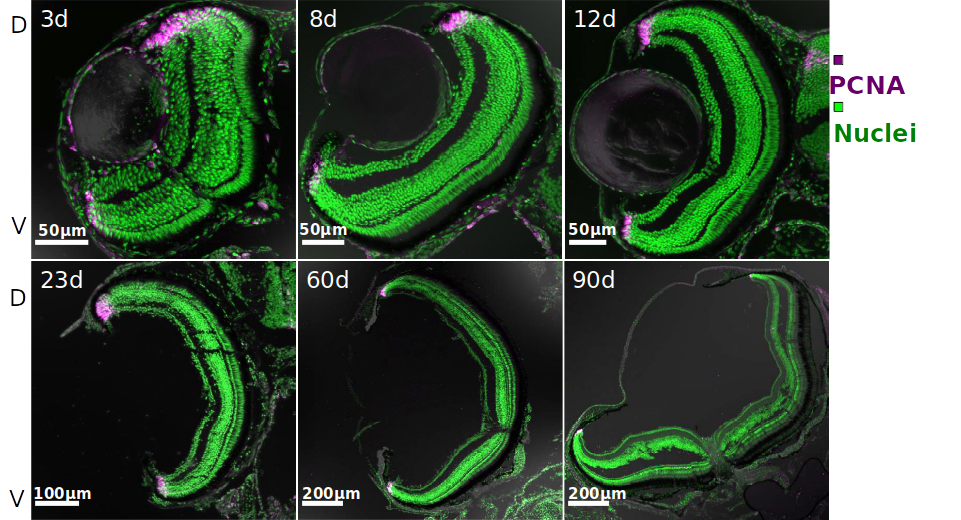
\includegraphics[width=1.1\textwidth]{cmz/cmz_schematic.png}}    
    \caption{{\bf Micrographic overview of CMZ development in \textit{D.rerio}, 3-90dpf}}
    Representative confocal micrograph maximum intensity projections (MIPs) of \SI{14}{\micro\metre} coronal eye cryosections, processed via IHC, of zebrafish of noted ages. Magenta – anti-PCNA staining. Green – Hoechst 33342 nuclear staining. Note changing scale bars.
    \label{cmz_dev_schematic}
    Methods in \autoref{ssec:PCNA}.
\end{figure}

We first estimate mean CMZ annulus population and retinal volume over the first year of life, in \autoref{CMZoverall}, panels A and C. The lack of growth observed in the first week of life suggests an initial quiescent period in the population history of the CMZ. Observations in \autoref{rysCMZontogeny}, showing CMZ RPCs are proliferating too slowly to be labelled by a 12 hour pulse of a thymidine analogue at 10dpf in the siblings of npat mutants, also suggest this quiescence. On the other hand, we have good confidence that retinal volume continues to grow over this time; 99.56\% of the marginal posterior mass of the mean 5dpf estimate is above the 3dpf mean, which may indicate any proliferative pause is too short to appear in the retinal volume data.

\begin{figure}[!h]
    \makebox[\textwidth][c]{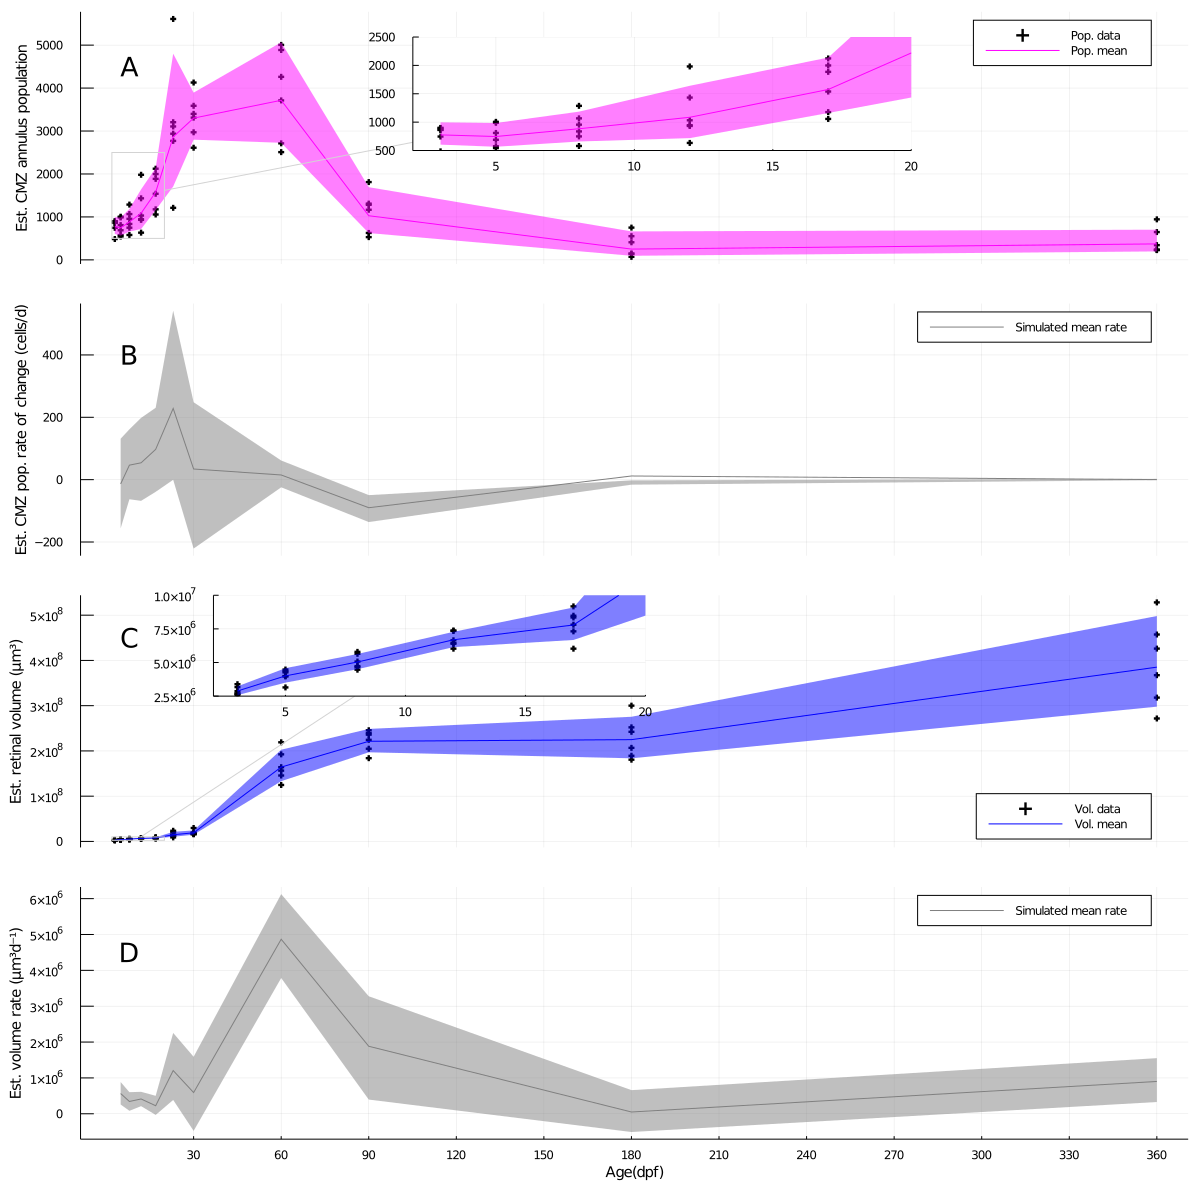
\includegraphics[width=1.\textwidth]{cmz/CMZoverall.png}}    
    \caption{{\bf Population and activity of the CMZ over the first year of \textit{D.rerio} life}}
    Panel A: Marginal posterior mean CMZ annulus population. Panel B: Marginal posterior mean retinal volume estimate. Insets in Panels A \& B display data from 3-17 dpf. Panel C: Marginal posterior mean of the proliferative index of the CMZ annulus, assayed by specified retinal neurons with incorporated thymidine from an 8hr pulse at the indicated ages. Panel D: Mean daily rate of volumetric increase of the neural retina, calculated as the difference in volumes between two ages over the number of elapsed days. All means are displayed in a band representing the $\pm 95 \%$ credible interval for the marginal posterior distribution of the mean.
    \label{CMZoverall}
    Methods in \autoref{ssec:CMZpopvolest}, \autoref{ssec:MCrates}.
    Code in \autoref{ssec:a10popsurvey}.
\end{figure}

The first two to three weeks of life (magnified in lens insets in panels A and C) see a slow build in both estimated CMZ annulus population and retinal volume compared to the large increase which follows. While zebrafish are better staged by size than age \cite{Parichy2009}, the onset of this growth seems to come earlier than the metamorphic transition from larval to juvenile stages at ~45dpf \cite{Singleman2014}. This raises the question of how the CMZ contributes to the retina during the critical period of exponential growth of the organism, between about 45 and 90dpf. It is plausible, for instance, that the growth of the CMZ population mainly reflects the increased cell cycle rate, with RPCs specifying at some steady rate, or that the CMZ builds itself up for a wave of increased niche exit and specification somewhat later, similarly to the sequence of events in the embryonic central retina.

To ascertain this timing, we simulated the mean daily rate of change of the CMZ annulus population and retinal volume, by performing Monte Carlo difference operations between samples from the marginal posterior means of subsequent timepoints. These simulated mean rates and their associated, empirically determined confidence intervals are plotted in \autoref{CMZoverall} panels B and D. These show the time-structure of the phenomenon; the increase in simulated daily CMZ population growth rate occurs before the increase in retinal volume, but the CMZ population estimate does not begin to drop off until 60dpf, by which time the majority of volumetric growth is complete. This seems to substantiate some combination of the scenarios outlined above: there is an early buildup of CMZ population around 18-30dpf, before CMZ RPCs begin to make their primary contribution to the retina between 30-60dpf, which seems to be characterised by much slower population growth and more rapid volumetric growth, implying steady and elevated specification and niche exit of RPCs. 

Subsequent to the bulk of the CMZ buildup and contribution to the retina, the population of the CMZ declines at about 39\% the rate of its peak ascent, with an estimated -90.1$\frac{cells}{d}$ by 90dpf. This thins out the CMZ population to below its inital value, spread out over a much larger peripheral annulus, for a much less dense mature CMZ. Interestingly, the 95\% CI on the marginal posterior mean of estimated retinal volume at 180 dpf (ranging from \SI{1.84E8}{\cubic\micro\metre} to \SI{2.75E8}{\cubic\micro\metre}) completely encompasses the 95\% CI on volume at 90dpf (\SI{1.96E8}{\cubic\micro\metre}-\SI{2.48E8}{\cubic\micro\metre}), while the 360dpf mean (\SI{3.85E8}{\cubic\micro\metre}) is greater than six standard deviations from the 180dpf mean (\SI{2.25E8}{\cubic\micro\metre}). This suggests a possible second period of quiescence from approximately 90-180dpf, followed by steady contribution to the retina without a buildup in the CMZ population subsequently.

Given this description, the ontogeny of the CMZ as a stem cell niche could be well-described by different phases of activity, with different rates of proliferation and specification. It is not immediately clear what sort of periodization is justified by the data. It seems plausible that as few as two phases could explain the data well enough: an initial phase of logarithmic growth, with short cell cycle time and lower exit rate of RPCs from the CMZ into the specified neural retina, followed by a second phase of decay with longer cycle time and higher exit rate. On the other hand, perhaps some of the data features noted above justify a more complex model that captures, for instance, the initial quiescent period, or the post-180dpf growth of the retina. Because this is a question of how much model structure is justified by our data, we may address it as a model selection problem.

\section{Two-phase periodization of postembryonic CMZ activity by phased difference equation modelling}
\label{sec:phaseGMC}
To perform our model selection task, we simulate the time-evolution of CMZ population and retinal volume. This requires initial values for the size of the simulated CMZ populations and the volumes of the simulated retinae they are associated with. Given the findings presented in \autoref{gausscorrelation}, we are justified in initializing CMZ population and retinal volume by independent samples from the Log-Normal models of their interindividual variability at 3dpf, the end of embryogenesis and the beginning of the period of CMZ-driven retinal growth. To produce new, simulated values of CMZ population and retinal volume, we apply a system of difference equations as follows, where $pop_n$ is the population at $n$ dpf, $CT$ is the mean cell cycle time of the population in hours, and $\epsilon$ is the proportion of the population at time $n-1$ that exits cycle and contributes to the volume of the specified neural retina, and $\mu_{cv}$ is the mean volume per cell contributed to the retina in \si{\cubic\micro\metre}:

\begin{equation}
    p_n=p_{n-1} \cdot 2^{\frac{24}{CT}} - p_{n-1} \cdot \epsilon
    \label{popeq}
\end{equation}

\begin{equation}
    v_n=v_{n-1} + p_{n-1} \cdot \epsilon \cdot \mu_{cv}
    \label{voleq}
\end{equation}

A model "phase" can then be defined by the $CT$ and $\epsilon$ parameters it applies to update the population and volume, over the appropriate number of days. The full parameterisation of a model with $p$ phases is given by $p$ pairs of $CT$ and $\epsilon$ values, and $p-1$ phase transition dates. $\mu_{cv}$, which is taken to apply equally to all phases, is estimated from 3 dpf nuclear measurements, as described in \autoref{ssec:CMZpopvolest}. This model is described further in \autoref{sec:CMZmodel}.

Given an initial population and volume sampled from the Log-Normal models of their interindividual distributions, \autoref{popeq} and \autoref{voleq} are be applied to these values to produce simulated sample measurements. Many such samples obtained by \hyperref[ssec:MonteCarlo]{Monte Carlo} can be used to estimate Log-Normal distributions for simulated CMZ populations and retinal volume, which can be used to score the model against observations. By defining prior distributions over the model parameters, we may sample from the prior to initialize a model ensemble. The ensemble can then be compressed by \hyperref[ssec:nested]{nested sampling}, moving each model-particle over the parameter space by Galilean Monte Carlo, as described in \autoref{ssec:GMC}. Using typical procedures applied in nested sampling \cite{Skilling2006}, we estimated the Bayesian evidence, maximum a posteriori model output, and marginal posterior distributions on parameters for 2 and 3-phase models.

\begin{figure}[!h]
    \makebox[\textwidth][c]{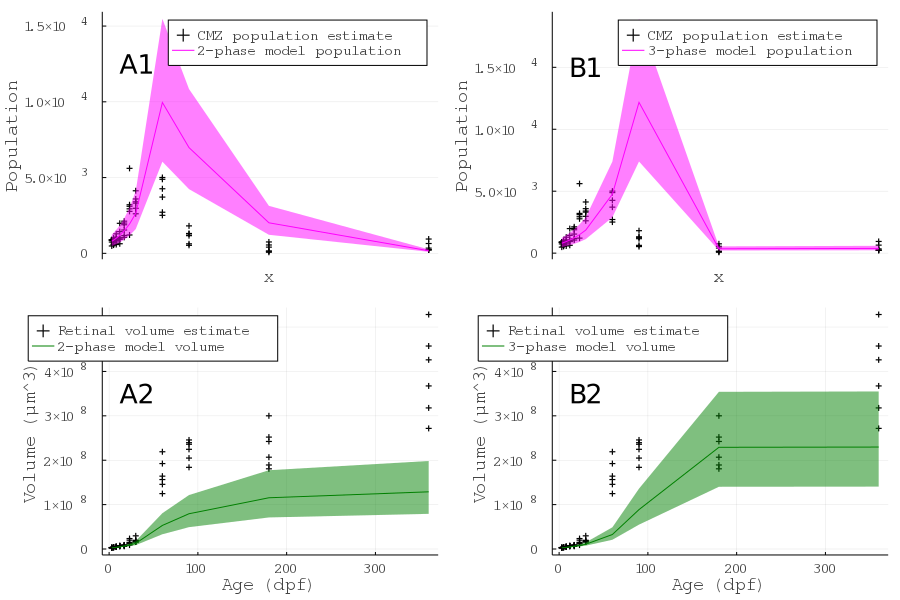
\includegraphics[width=1.2\textwidth]{cmz/a10pMAP.png}}    
    \caption{{\bf Maximum a posteriori output of periodization models}}
    \label{phaseMAPout}
    Population and volume estimates from observations (crosses) plotted with mean $\pm$ 95\% probability density model output, for the 2-phase model (A panels) and 3-phase model (B panels). A1,B1: population estimates. A2,B2: volume estimates. Insets provide magnified views of data from the first 30dpf.
    Methods in \autoref{ssec:GMCev}.
    Code in \autoref{ssec:a10periodisation}.
\end{figure}

The maximum a posteriori model output shows the major problem with this simple model; the model relationship between changes in CMZ population and changes in volume breaks down rapidly. That is, the later volume estimates are too large for the CMZ to produce, given the calculated cellular volume ($\mu_{cv}$) at 3dpf. The models fit the early population and volume data better, but the population peak is dragged upward to produce more-likely volume output at later ages. While it is possible that the later CMZ contributes more volume per neuron to the cellular retina, it seems more likely that the volume approximation applies better to more-nearly spherical eyes at younger ages, than to the flattened eyes of later ages. When we tried floating $\mu_{cv}$ as a variable within the model, the MAP results were similar (data not shown), suggesting that a constant value for $\mu_{cv}$ across ages is the problem in achieving good model fits, not the particular value chosen. This reinforces the idea that the problem relates to the breakdown of the retinal volume estimate at later ages.

While this limitation prevents either model from explaining the combined estimate datasets very well, they are in this sense under the same constraint, and so some inference about the number of phases justified by the data is still possible. Evidence estimates for the 2-phase and 3-phase models, given these data, are presented in \autoref{phasetable}. There are greater than 3500 orders of magnitude more evidence for the 2-phase model; this result has over 200 standard deviations of significance. This reflects the expanded parameter space in the 3-phase model, which has 8 parameters, compared to the 2-phase models' 5. The additional flexibility afforded by the 3rd phase in fitting the later volume data is unable to overcome the evidentiary penalty associated with the larger parameter space. We conclude that the 2-phase model is a better-justified description of these data.

\begin{table}[!ht]
    \centering
    \caption{{\bf Evidence favours a 2-phase periodization of CMZ activity}}
    \begin{tabular}{|l|l|l|l|} \hline 
        {\bf 2-phase logZ} & {\bf 3-phase logZ} & {\bf logZR} & {\bf $\sigma$ Significance}\\ \hline
        \textbf{-7147.3 ± 9.4} & -10743.0 ± 13.0 & 3596.0 ± 16.0 & 227.624\\ \hline
        \end{tabular}
    \begin{flushleft} logZ: logarithm of p(D), the marginal likelihood of the data, or model evidence. logZR: evidence ratio; positive ratios in favour of the 2-phase model. Largest evidence value bolded.
    Methods in \autoref{ssec:GMCev}.
    Code in \autoref{ssec:a10periodisation}.
    \end{flushleft}
    \label{phasetable}
\end{table}

While the parameter estimates associated with these models are clearly unreliable, they are useful to inspect in for comparison to the simulations to follow. We present the parameterization of the MAP model output displayed above in \autoref{phaseMAPtable}. Unsurprisingly, the selected 2-phase model begins with a first phase of rapid proliferation, with a $CT$ of 14.5 hr, followed by a second, slower phase of 17.5 hr. The imputed exit rate $\epsilon$ is greater than 200\% of the day's starting population in the first phase, suggesting that new cells exit the CMZ after about 12 hours, around one cycle, while the second phase exit rate is lower, with 160\% of the day's starting population exiting the CMZ, again suggesting a residency time of about one cycle. The imputed phase transition age is about 23dpf. Due to the volume estimate problem noted above, it is reasonable to believe that the $CT$ estimates are likely too short, the $\epsilon$ estimates too high, all favoured in order to produce higher volume estimates at later ages.

\begin{table}[!ht]
    \centering
    \caption{{\bf Maximum a posteriori parameter estimates for periodization models}}
    \begin{tabular}{|l|l|l|}
        \hline
        {\bf Parameter} & {\bf 2-phase MAP} & {\bf 3-phase MAP}\\ \hline
        Phase 1 $CT$ (h) & 14.5 & 14.9\\ \hline\
        Phase 1 $\epsilon$ & 2.02 & 1.95\\ \hline
        Phase 2 $CT$ (h) & 17.5 & 75.6\\ \hline
        Phase 2 $\epsilon$ & 1.6 & 0.29\\ \hline
        Phase 3 $CT$ (h) & NA & 68.4\\ \hline
        Phase 3 $\epsilon$ & NA & 0.27\\ \hline
        Transition 1 age & 23.2 & 47.9\\ \hline
        Transition 2 age & NA & 179.4\\ \hline
    \end{tabular}
    \begin{flushleft}
        $CT$: cycle time.
        $\epsilon$: niche exit rate.
        Methods in \autoref{ssec:GMCev}.
        Code in \autoref{ssec:a10periodisation}.    
    \end{flushleft}
    \label{phaseMAPtable}
\end{table}

Because nested sampling produces weighted samples from the posterior, we can estimate posterior distributions on parameters. We did so by kernel density estimation, to investigate whether the marginal posterior distributions for the selected model are polymodal. This can reveal how the evidence supports multiple hypotheses about the parameters of the two imputed phases. Kernel density estimates (KDEs) for marginal posterior distributions on the 2-phase models' parameters are presented in \autoref{phasemarginals}. 

These estimates reveal monomodal posterior distributions over the parameters. $CT$ posteriors are well constrained to a small part of the sampling space (left panels, X axes, and top right panel), with the MAP parameter estimates given in \autoref{phaseMAPtable} falling within the most dense regions. However, it is evident that the data do not constrain phase exit rates $\epsilon$ (left panels, Y axes) very well. That is, the marginal posterior probability distributions for these parameters are very widely spread.  The marginal posterior distribution on the age at which the transition between phases occurs is plotted in the bottom right of \autoref{phasemarginals}; the KDE suggests that the age of phase transition is likely around 23 dpf.

\begin{figure}[!h]
    \makebox[\textwidth][c]{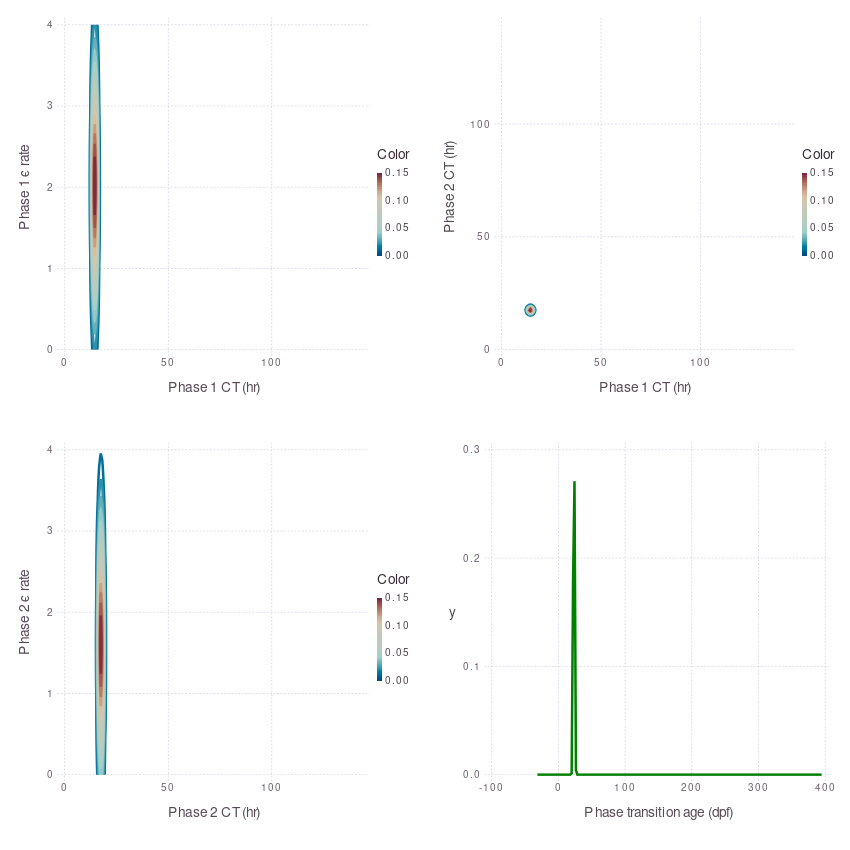
\includegraphics[width=.8\textwidth]{cmz/a10pmarginals.png}}    
    \caption{{\bf Kernel density estimates of marginal posterior parameter distributions, 2-phase model}}
    Prior distributions (magenta) apply to parameters of both phases. Maximum a posteriori model parameterisation indicated by vertical lines.
    Panel A: Marginal posterior distributions on Phase 1 and 2 $CT$ cycle time parameters. 
    Panel B: Marginal posterior distributions on Phase 1 and 2 $\epsilon$ niche exit rate parameters.
    Panel C: Marginal posterior distribution on Phase 1 to 2 transition age parameter.
    \label{phasemarginals}
    Methods in \autoref{ssec:GMCkde}.
    Code in \autoref{ssec:a10periodisation}.    
\end{figure}

The lower exit rate associated with MAP second phase highlights the fact that the relative cycle time or exit rate between phases is irrelevant to the overall behaviour of the system. What matters is whether the cycle time and exit rate within a phase produce a growing or shrinking CMZ. We conclude that, while our global model of CMZ population and volumetric retinal contribution is too flawed to make good parameter estimates, a 2-phase model of this activity is better substantiated by the evidence than a 3-phase model. We proceed on this basis, tentatively accepting the 2-phase model, and taking up the idea of the "slice model" introduced in \autoref{ssec:slice}, to investigate modelling the CMZ RPC population more concretely, directly from sectional observations, rather than from the calculated population and retinal volume estimates presented above.

\FloatBarrier

\section{Phased slice-models of CMZ population dynamics suggest subtle shifts across stable-population contour}
\label{sec:sliceGMC}

In the course of the preceding investigations, it became apparent that the CMZ population asymmetry mentioned in \autoref{chap:SMMEoutro} was not a static phenomenon, with the dorsal lobe of the CMZ annulus being consistently more populous than the ventral lobe, as generally implied by the sources covered in \autoref{chap:RPCreview}. Rather, both the extent and orientation of asymmetry change over time. Sectional population totals for the dorsal and ventral CMZ are presented in \autoref{DVontology}, Panel A, alongside the related intra-individual asymmetry ratio in Panel B. The initially pronounced dorsal population and reduced ventral population both seem to go through the overall boom-bust progression of CMZ population, but their relative proportion within individuals reverses itself over the period from 17-90dpf. We also observed a similar phenomenon occurring across the naso-temporal axis over the same time period (\autoref{NTontology}).

\begin{figure}[!h]
    \makebox[\textwidth][c]{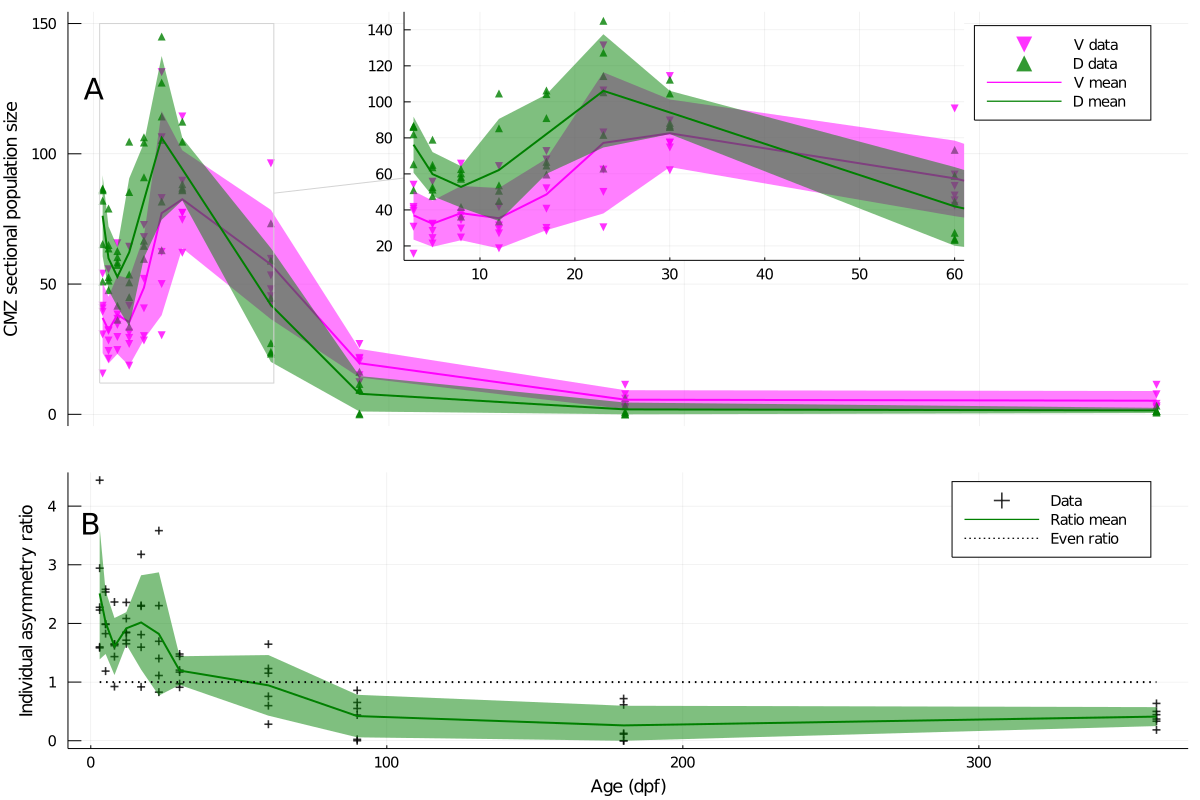
\includegraphics[width=1.2\textwidth]{cmz/DVontology.png}}    
    \caption{{\bf Developmental progression of dorso-ventral population asymmetry in the CMZ.}}
    Marginal posterior distribution of mean dorsal (D) and ventral (V) population size in 14$\mu$m coronal cryosections (panel A) or intra-individual D/V count asymmetry ratio (panel B), $\pm 95\%$ credible interval, n=5 animals per age. Data points represent mean counts from three central sections of an experimental animal's eye. 
    \label{DVontology}
    Methods in \autoref{ssec:PCNA}.
    Code in \autoref{ssec:a10dvratio}. 
\end{figure}

Inspected closely, these data provide a possible rationale for the reversal of asymmetry in the proliferative dynamics of the niche itself: the sectional (or ``slice'') population of the dorsal CMZ is increasing beyond its postembryonic minimum by 12dpf, while the ventral CMZ takes until 17dpf to exhibit a noticeable increase in size; moreover, the peak dorsal population is achieved by 23dpf, whilst ventrally the peak is only achieved at 30dpf. This suggests that the dorsal and ventral CMZ populations may undergo similar, time-shifted processes of proliferation from different starting populations. If this is so, an explanation for this time-shifted phenomenon could have fundamental relevance to predicting and controlling the proliferative behaviour of peripheral RPCs and stem cells.

To test this hypothesis, we used a ``slice model'' of the CMZ, where the thickness of the slice is taken to be the same as the observed cryosection thickness (\SI{14}{\micro\metre}). The population of the CMZ is modelled with a difference equation, as above, but with an additional exit term representing lateral, circumferential contributions of the CMZ to the generation of new, adjacent ``slices''. The value of this term is calculated from the difference in CMZ annulus diameter over the calculated time period, as implied by a power-law model of lens growth fitted to observations, discussed in \autoref{sec:lenspopest}. The resultant difference equation is \autoref{sliceeq}. Terms are as defined above, except that $p_n$ is the sectional population at $n$ dpf, and not the total CMZ annulus population; additionally, $\eta$ is defined as the daily circumferential exit rate implied by the power-law model. The model is detailed in \autoref{sec:slicemodel}.

\begin{equation}
    p_n=p_{n-1} \cdot 2^{\frac{24}{CT}} - p_{n-1} \cdot \epsilon - \eta
    \label{sliceeq}
\end{equation}

We reasoned that, if the phase transition occurs earlier in the dorsal CMZ than in the ventral CMZ, there should be some informational gain in separating these observations vs. both slices being governed by one model. We therefore estimated the evidence, MAP, and posterior marginals for 2-phase models given the sectional dorsal and ventral populations, both combined and as separately-parameterised slices. To focus on the most informative subset of the data for our hypothesis, we restricted this analysis to the population data within the first three months of life.

The slice model proves to have greater success at explaining sectional counts than the whole-eye model does at explaining the annulus population estimates; maximum a posteriori model output is presented in \autoref{dvMAPout}. In particular, all of the models adequately represent the early decline in sectional populations, arising from rapid early growth of the eye that exceeds the CMZs' proliferative capacity, without further ado; there is no justification for a separate early quiescent period, as suggested above.

\begin{figure}[!h]
    \makebox[\textwidth][c]{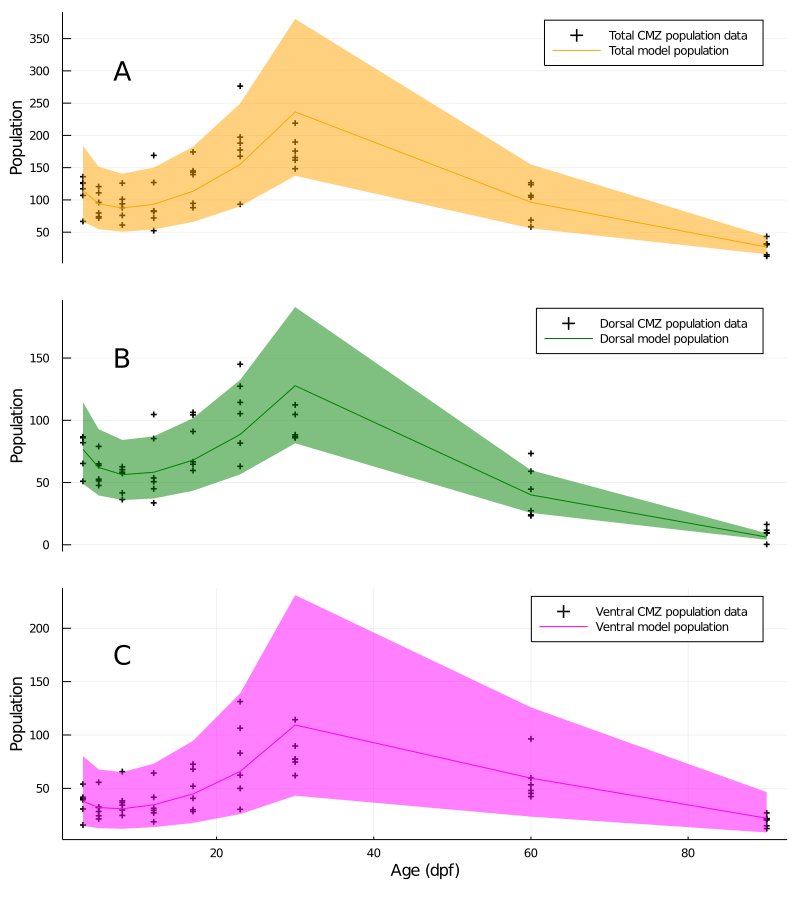
\includegraphics[width=1.0\textwidth]{cmz/a10dvMAP.png}}    
    \caption{{\bf Maximum a posteriori output of total, dorsal, and ventral CMZ slice models}}
    \label{dvMAPout}
    Population and volume estimates from observations (crosses) plotted with mean $\pm$ 95\% probability density model output, for the total CMZ population model (panels A \& B), dorsal CMZ population model (panel C), and ventral CMZ population model (panel D).
    Methods in \autoref{ssec:GMCev}.
    Code in \autoref{ssec:a10dvslice}. 
\end{figure}

The hypothesis that there is a time-shift in the phase transition across the dorso-ventral axis is not supported by these models. First, the evidence estimates demonstrate that we are not justified in separating the dorsal and ventral populations. The total-population slice model receives greater than 500 orders of magnitude more evidence than the joint evidence for the separate dorsal and ventral models, with greater than 20 standard deviations of significance, as displayed in \autoref{dvtable}. It is interesting to note that the evidence for the dorsal model (-579.9 ± 0.9) is substantially less than for the ventral model (-328.9 ± 0.5). This may indicate a causal influence on the dorsal population that is neither in the model nor acting on the ventral population, or it may be an uninformative sampling effect. A second indication that this hypothesis is unsupported are the MAP model parameter values, summarized in \autoref{dvMAPtable}. The dorsal MAP transition is actually later than the ventral date, which further suggests the original model-idea of a time-shifted late ventral phase change is unsupported by these data.

\begin{table}[!ht]
    \centering
    \caption{{\bf Evidence favours a combined slice model over separate dorsal and ventral models}}
    \begin{tabular}{|l|l|l|l|l|}
        \hline
        {\bf Combined D/V model logZ} & {\bf Separate D/V model logZ} & {\bf logZR} & {\bf $\sigma$ Significance}\\ \hline
        \textbf{-874.3 ± 1.2} & -908.8 ± 1.0 & 34.5 ± 1.6 & 21.9\\ \hline
    \end{tabular}
    \begin{flushleft} logZ: logarithm of p(D), the marginal likelihood of the data, or model evidence. logZR: evidence ratio; positive ratio in favour of the combined model. Largest evidence value bolded.
    Methods in \autoref{ssec:GMCev}.
    Code in \autoref{ssec:a10dvslice}.     
    \end{flushleft}
    \label{dvtable}
\end{table}

The MAP parameters for the combined slice model suggest that those found for the 2-phase MAP in \autoref{phasemarginals} overstate cell cycle speed and exit rate. The combined slice model gives $CT$s of 34.4 and 23.3 hours for the first and second phases, compared to 14.5 and 17.5 estimated for the whole-eye model. Moreover, the niche exit rates $\epsilon$ are estimated at .54 and 1.07 for the combined slice model, compared to 2.02 and 1.6 for the whole-eye model. The values of the slice model seem more realistic in general; it seems unlikely that over one day, fully 200\% of the day's starting CMZ population has exited the niche and entered the specified neural retina, for instance, as implied by the first phase exit rate of the whole-eye model. As well, given that $CT$ represents an average cycle time over a heterogenous population of progenitors, many of whom are becoming postmitotic, $CT$ values over 24 hr seem much more plausible than the ~15 hr parameter required for the whole-eye model to produce its unrealistically exaggerated population.

\begin{table}[!ht]
    \centering
    \caption{{\bf Maximum a posteriori parameter estimates for slice models}}
    \begin{tabular}{|l|l|l|l|}
        \hline
        {\bf Parameter} & {\bf Combined MAP} & {\bf Dorsal MAP} & {\bf Ventral MAP}\\ \hline
        Phase 1 $CT$ (h) & 34.4 & 33.6 & 17.8\\ \hline
        Phase 1 $\epsilon$ & 0.54 & 0.57 & 1.43\\ \hline
        Phase 2 $CT$ (h) & 23.3 & 35.0 & 11.2\\ \hline
        Phase 2 $\epsilon$ & 1.07 & 0.67 & 3.42\\ \hline
        Transition age & 32.2 & 41.0 & 27.8\\ \hline
        \end{tabular}
    \begin{flushleft}
        $CT$: cycle time.
        $\epsilon$: niche exit rate.
        Methods in \autoref{ssec:GMCev}.
        Code in \autoref{ssec:a10dvslice}.    
    \end{flushleft}
    \label{dvMAPtable}
\end{table}

The marginal posterior distributions of the total slice model, presented in \autoref{dvmarginals}, are substantially more polymodal than those in \autoref{phasemarginals}. This illustrates how data can support multiple hypotheses about model parameters to different degrees. When the phase marginal $CT$ and $\epsilon$ are plotted together, they display the characteristic density curves displayed in Panels A and B of \autoref{dvmarginals}. This supplies the most interesting information available by estimating this slice model. Firstly, the posterior marginal distributions of the first and second phase are very close to one another. Importantly, when the $CT$-$\epsilon$ contour which gives a stable population is plotted (dotted lines), it becomes obvious that the bulk of the first phase posterior lies just under this curve, while the bulk of the second phase lies just above it. This strongly suggests that the population dynamics of the CMZ may be characterised by a relatively subtle shift across the stable population contour, rather than distinct phases.

It should be noted that the MAP estimate does not occupy the most credible KDE kernel. An important property of nested sampling is that the accuracy of evidence calculations is traded off against the accuracy of estimating the posterior distribution \cite{Speagle2019}, as noted in \autoref{ssec:GMC}. Since we have here prioritized evidence estimation, this is one cause of this discrepancy; the MAP models themselves may have relatively little weight in the KDE estimates. The oversampling of the prior periphery noted in \autoref{chap:GMC}, as well as the very significant polymodality of the model posteriors displayed in Supplementary \autoref{polymodality} also contribute to this problem\footnote{A more conventional approach to reporting posterior estimates is to provide the mean and variance of the distribution, rather than the position of the most likely model in the MAP ensemble. We have eschewed this because of the tendency of \path{GMC_NS} to oversample the prior volume.}.

\begin{figure}[!h]
    \makebox[\textwidth][c]{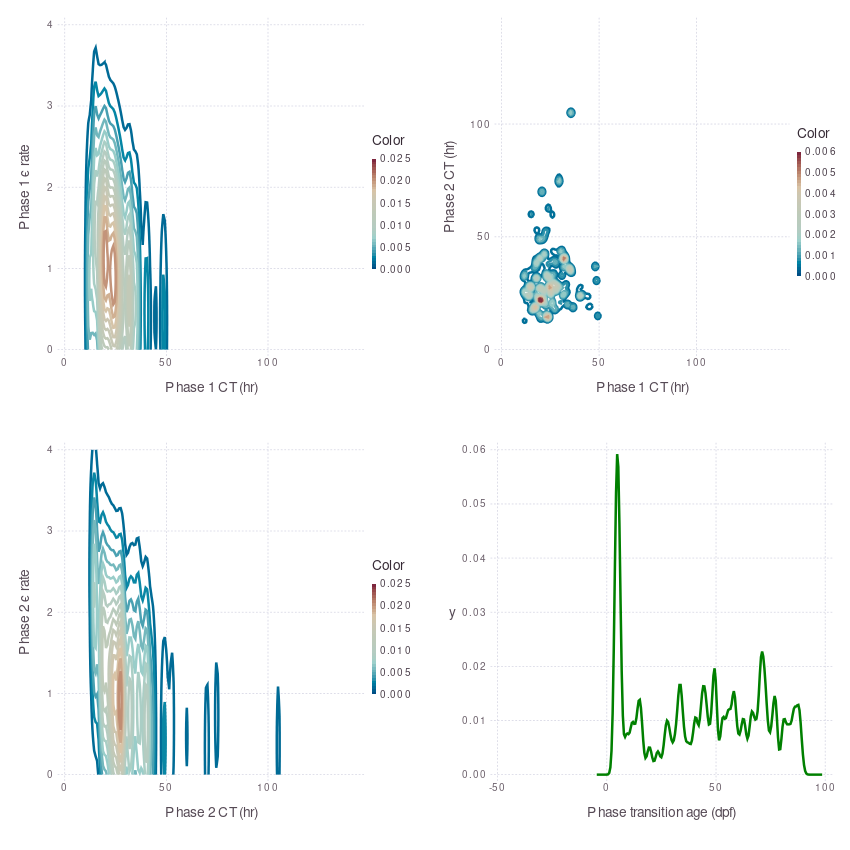
\includegraphics[width=1.\textwidth]{cmz/a10dvmarginals.png}}    
    \caption{{\bf Kernel density estimates of marginal posterior parameter distributions, total slice model}}
    Panel A: Bivariate KDE of Phase 1 posterior $CT$ vs. $\epsilon$ density. Univariate marginals, with priors, are plotted to the left and below of the bivariate panel.

    Panel B: Bivariate KDE of Phase 2 posterior $CT$ vs. $\epsilon$ density. Univariate marginals, with priors, are plotted to the left and below of the bivariate panel.

    Panel C: Univariate KDE of Phase 1-2 transition age.

    Line height (univariate panels) or color scale (bivariate panels) indicates the estimated marginal posterior density present at the indicated parameter value. MAP parameters are given with magenta crosses (bivariate panels).
    \label{dvmarginals}
    Methods in \autoref{ssec:GMCkde}.
    Code in \autoref{ssec:a10dvslice}.    
\end{figure}

On the basis of the marginal posterior analysis of this model, we suspected that separately parameterised phases is not the best available description of the data. In particular, the relatively small shifts across the balanced population contour implied by the posterior distributions argues strongly for a model with one phase with a slowly decaying cycle rate.

\FloatBarrier

\section{Slice models of decaying cell cycle support anatomical homogeneity of RPC behaviour}
\label{sec:decaymodel}

To model the CMZ as a population of cells with a continuously lengthening cell cycle time, we modify the slice model described above by removing the phases and introducing an exponential decay equation for cycle time. This results in a slice model with three parameters: the initial cycle time ($CT_{i}$), a constant exit rate ($\epsilon$), and a decay constant ($\kappa$). Population values are updated daily as per \autoref{sliceeq}, including the use of the lens model, except that the cycle time $t$ days after initialising is determined by $CT_{t}=CT_{i} \cdot e^{\kappa \cdot t}$. More detail is provided in \autoref{sec:decaymodel}

\begin{figure}[!h]
    \makebox[\textwidth][c]{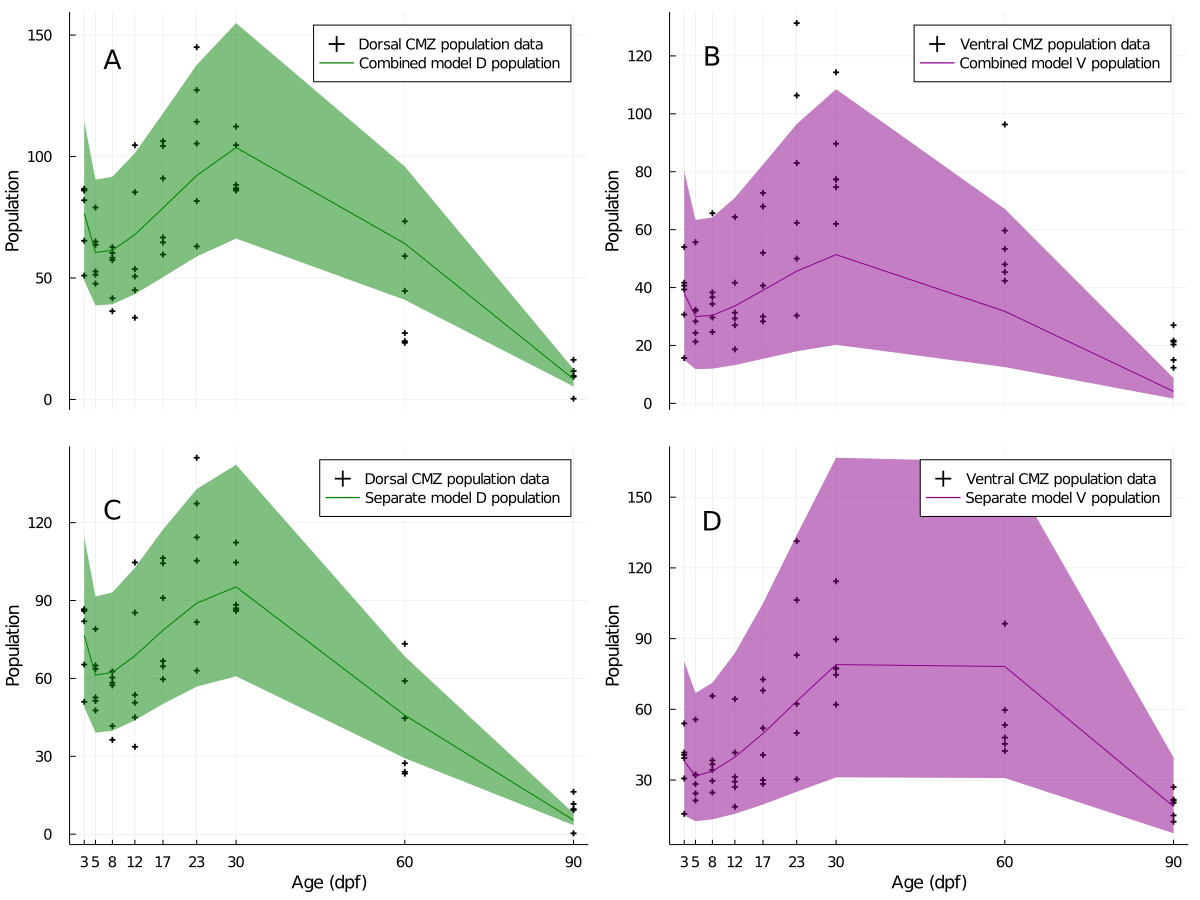
\includegraphics[width=1.0\textwidth]{cmz/a10dvdecayMAP.png}}    
    \caption{{\bf Maximum a posteriori output of total, dorsal, and ventral CMZ decay models}}
    \label{decayMAPoutput}
    Population and volume estimates from observations (crosses) plotted with mean $\pm$ 95\% probability density model output, for the total CMZ population model (panel A \& B), dorsal CMZ population model (panel C), and ventral CMZ population model (panel D).
    Methods in \autoref{ssec:GMCev}.
    Code in \autoref{ssec:a10dvdecayslice}. 
\end{figure}

We performed the same sampling routine on the same 3-90dpf dataset used for the earlier slice models, to enable direct comparison between them. The evidence calculations are presented in \autoref{decayevtable}. The combined decay model substantially outperforms the combined slice model selected above, as well as separate decay models. Therefore, the model evidence supports the use of the decay model for describing RPC behaviour in general; however, there is insufficient evidence to distinguish between dorsal and ventral populations using this model.

\begin{table}[!ht]
    \centering
    \caption{{\bf Evidence supports separate dorsal and ventral decay models}}
    \begin{tabular}{|l|l|l|l|l|l|}
        \hline
        {\bf Combined slice logZ} & {\bf Combined decay logZ} & {\bf D/V decay logZ} & {\bf decay logZR} & {\bf $\sigma$ Sig.}\\ \hline
        -874.3 ± 1.2 & {\bf -762.6 ± 0.7} & -794.6 ± 0.8 & 32.0 ± 1.1 & 29.3\\ \hline
    \end{tabular}
    \begin{flushleft} logZ: logarithm of p(D), the marginal likelihood of the data, or model evidence. logZR: evidence ratio between separate D/V decay models and a combined decay model; positive ratio in favour of the combined model. Combined slice model from \autoref{dvtable} included in left column for comparison. Largest evidence value bolded.
    Methods in \autoref{ssec:GMCev}.
    Code in \autoref{ssec:a10dvdecayslice}.     
    \end{flushleft}
    \label{decayevtable}
\end{table}

MAP model output for the combined and separate decay models is presented in \autoref{decayMAPoutput}, while the MAP parameter estimates are summarised in \autoref{decayMAPtable}. Generally speaking, the values estimated for the parameters of the decay model suggest a much gentler proliferative schedule for RPCs, with initial cycle times measured in days, and daily niche exit rates of between 15-30\% of the RPC population. Cumulative thymidine analogue labelling results, presented below, suggest these values are unrealistically long. Interestingly, MAP parameterisations for the split Dorsal and Ventral models do not imply that dorsal RPCs are more active than those found ventrally. Probably, if consistent regional biases in CMZ RPC behaviour exist, better data would be required to constrain niche exit rate. Indeed, it seems likely that the lack of effective constraint on the model's niche exit rate $\epsilon$ allows for the unrealistically long $CT_{i}$ suggested by both combined and separate decay models. We conclude that explanations invoking differences in CMZ RPC behaviour across morphological axes  cannot be supported with our models and datasets, indicating that morphological homogeneity of these parameters is descriptively adequate at this level.

\begin{table}[!ht]
    \centering
    \caption{{\bf Maximum a posteriori parameter estimates for decay models}}
    \begin{tabular}{|l|l|l|l|}
        \hline
        {\bf Parameter} & {\bf Combined MAP} & {\bf Dorsal MAP} & {\bf Ventral MAP}\\ \hline
        $CT_{i}$ (h) & 52.0 & 69.7 & 62.1\\ \hline
        $\kappa$ decay& 0.0067 & 0.0124 & 0.0091\\ \hline
        $\epsilon$ exit& 0.276 & 0.164 & 0.189\\ \hline
    \end{tabular}
    \begin{flushleft}
        $CT_{i}$: Initial cycle time.
        $\kappa$: Exponential cycle time decay constant.
        $\epsilon$: niche exit rate.
        Methods in \autoref{ssec:GMCev}.
        Code in \autoref{ssec:a10dvdecayslice}.    
    \end{flushleft}
    \label{decayMAPtable}
\end{table}

Marginal distributions on these parameters are summarised in \autoref{decaymarginals}. We again note that the data are informative for parameters of cell cycle ($CT_{i}$ and $\kappa$), but give little information regarding niche exit rate. The MAP models found by GMC are well outside the kernel density estimates of the posterior distributions supplied by nested sampling this model. It is not clear why this should consistently be the case. The decay model may be characterised by small, high credibility modes that are outside the bulk of the less credible posterior mass; possibly, these are underweighted if they come late in the nested sampling process. In any case, the posterior marginals seem to confirm that there is little reason to separately distinguish dorsal and ventral subpopulations of CMZ RPCs.

\begin{figure}[!h]
    \makebox[\textwidth][c]{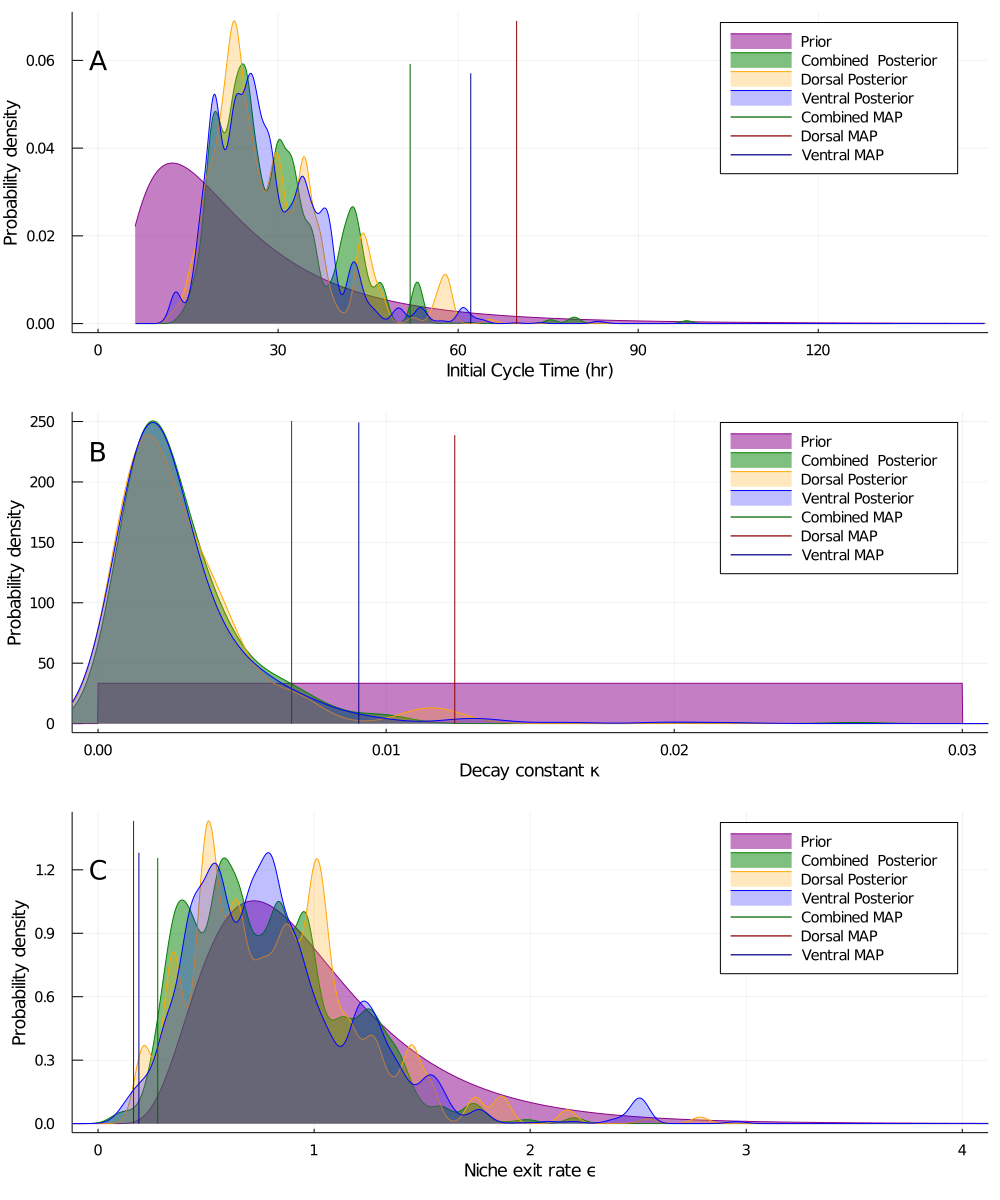
\includegraphics[width=.8\textwidth]{cmz/a10decaymarg.png}}    
    \caption{{\bf Kernel density estimates of marginal posterior parameter distributions, decay models}}
    \label{decaymarginals}

    Panel A: Marginal prior and posterior distributions on $CT_{i}$.
    Panel B: Marginal prior and posterior distributions on $\kappa$.
    Panel C: Marginal prior and posterior distributions on $\epsilon$.

    MAP model parameters are given by vertical lines.
    Methods in \autoref{ssec:GMCkde}.
    Code in \autoref{ssec:a10dvdecayslice}.    
\end{figure}

\FloatBarrier

\section{Bayesian inference of cycle parameters from cumulative thymidine labelling experiments supports slice model cycle time estimates}
\label{ssec:CMZcumedu}

We sought to confirm the plausibility of the $CT$ estimates obtained from modelling CMZ population measurements with an independent line of evidence. We  examined 3dpf CMZ RPCs cumulatively labelled with a 10.5 hour pulse of the thymidine analogue EdU \cite{Chehrehasa2009}. We used the Empirical Bayes approach to estimate the evidence for separate Nowakowski-style \cite{Nowakowski1989} linear models for the dorsal and ventral CMZ, against a model for both subpopulations combined. While this model is inadequate for reasons outlined in \autoref{chap:SMME}, it can serve to substantiate the first phase cycle time parameter. These results are summarized in \autoref{cumEdUtable}, with the relevant linear regressions displayed in Supplementary \autoref{cumEdUlinreg}.

\begin{table}[!ht]
    \centering
    \caption{{\bf Evidence favours whole-CMZ linear cycle models over separate D/V models}}
    \begin{tabular}{|l|l|l|l|} 
        \hline {\bf Model} & {\bf Implied $T_c$ (hr)} & {\bf Implied $T_s$ (hr)} & {\bf logZ}\\ \hline 
        Dorsal & 14.7 $\pm$ 1.6 & 1.38 $\pm$ 0.76 & 7.778\\ \hline 
        Ventral & 14.0 $\pm$ 1.2 & 0.8 $\pm$ 0.58 & 15.202\\ \hline
        Combined & 14.6 $\pm$ 1.1 & 1.25 $\pm$ 0.53 & {\bf26.165}\\ \hline
    \end{tabular}
   
    \begin{flushleft} $T_c$: calculated cell cycle time. $T_s$: calculated s-phase length. logZ: logarithm of p(D), the marginal likelihood of the data, or model evidence.  Largest evidence value bolded.
    Methods in \autoref{ssec:CMZEmpBayes}.
    Code in \autoref{ssec:a25dvlinreg}.    

    \end{flushleft}
    \label{cumEdUtable}
\end{table}

Firstly, there are approximately 3 orders of magnitude of evidence in favour of the combined model vs. the joint evidence for separate models (ie. 26.165 vs. 22.980). In general, this suggests that there is little traction to be gained by separating these observations along the D/V axis. The Nowakowski-calculated cell cycle time $T_c$ for the combined model, 14.6 $\pm$ 1.1 hr, includes the whole-eye MAP first phase $TC$, 14.5 hr, within one standard deviation. This suggests the Nowakowski model has similar problems to the whole-eye models presented in \autoref{phaseMAPout}, substantially overstating cycle rate. Calculated S phase lengths are also unrealistically short. Finally, the data seem to diverge from a linear trend toward the end of the pulse (see \autoref{cumEdUlinreg}), showing the limitations of this model.

Because the Nowakowski model is clearly inadequate for estimating RPC cycle parameters in the CMZ, we implemented a cell-based cycle simulator, similar to those in \autoref{chap:SMME}, to model discrete cumulative thymidine labelling counts, in lineages with explicitly simulated cycle events. This model is described further in \autoref{sec:thymidinemodel}. The MAP model output for this model is presented in \autoref{a25MAP}; it does a better job of describing the observations than the Nowakowski method, particularly at the earliest timepoints, due to simulation of cycle time correlation between sibling cells, as well as detector sensitivity. 

\begin{figure}[!h]
    \makebox[\textwidth][c]{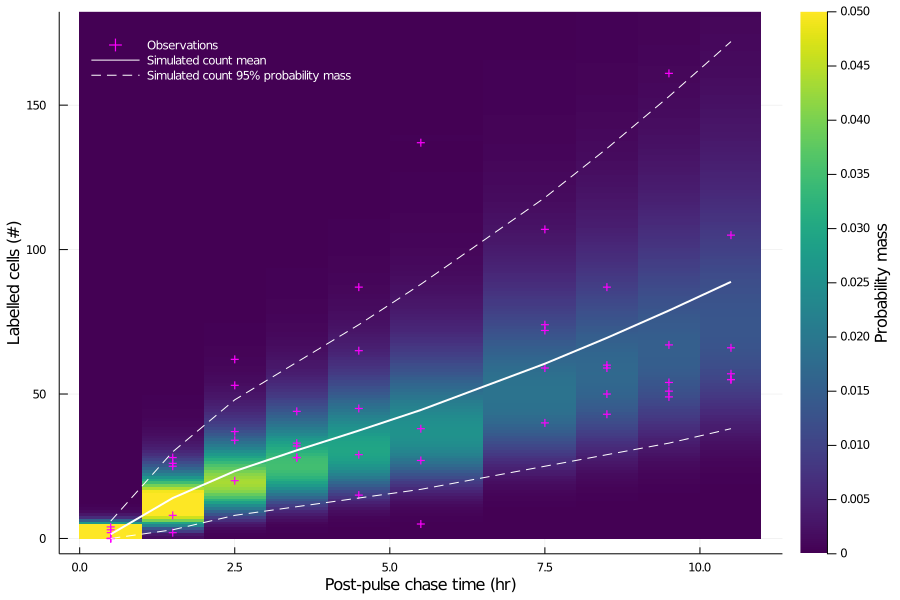
\includegraphics[width=1.\textwidth]{cmz/a25MAP.png}}    
    \caption{{\bf MAP model output and observations for thymidine slice model of 3dpf cumulative EdU labelling}}
    Count of EdU-positive cells observed in 14\si{\micro\metre} coronal cryosections through \textit{Danio} CMZs, at indicated chase times, during a 10 mM EdU pulse (magenta crosses), overlaid with MAP model output. Probability mass distribution of the discrete non-parametric output is shown by color scale; yellow values include counts with >.05 mass. Output mean and 95\% mass are indicated by solid and dashed white lines.

    Methods in \autoref{ssec:RyscumEdU}, \autoref{ssec:GMCev}. Code in \autoref{ssec:a25thymidinesim}.
    \label{a25MAP}
\end{figure}

KDE estimation of marginal distributions over the model parameters are presented in \autoref{a25marg}. These estimates give us a clear picture of what can be learnt from these data; mean cycle time and the length of S phase as a fraction of the cycle time are significantly compressed relative to the prior, but little can be gleaned about the variance of the cycle time distribution, and almost no information is available about the G1 or sister shift fraction. That is, for the parameters which the data offer little information, the posterior distribution correctly collapses back onto the prior, which indicates that this approach adequately copes with unconstrained parameters\footnote{The model is overparameterised relative to the available dataset. This was done deliberately to allow the model to be used with richer data than were available here; however, it does have the effect of making sampling against these observations less efficient than is achievable.}.

\begin{figure}[!h]
    \makebox[\textwidth][c]{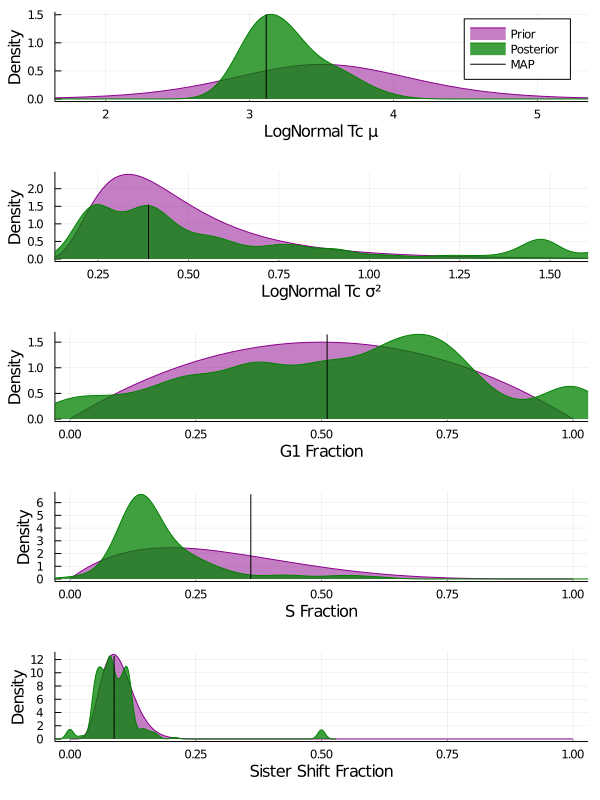
\includegraphics[width=.8\textwidth]{cmz/a25marginals.png}}    
    \caption{{\bf Marginal posterior distributions for thymidine slice model}}
    Marginal prior (magenta) and posterior (green) distributions on thymidine simulator cycle parameters, noted on the x axis. MAP model parameters are displayed with vertical black lines.

    Methods in \autoref{ssec:RyscumEdU}, \autoref{ssec:GMCkde}. Code in \autoref{ssec:a25thymidinesim}
    \label{a25marg}
\end{figure}

The MAP parameters for the LogNormal distribution of cycle times produces a mean cycle time of 24.0 hr. This seems to be a more realistic estimate of RPC cell cycle time, and tends to support the longer values estimated in the slice models, although it does suggest the 50+ hour $CT_{i}$ estimates for the decay models may be excessively long. Furthermore, this result supports our observation in \autoref{PerLineageFig} that the He model examined in \autoref{chap:SMME} substantially overstates the per-lineage proliferative rate of RPCs, at least in the CMZ; the He model's mean cycle time of 6 hours is much too fast to correctly model this population. It is likely that most reports of similar, very short cycle times for embryonic RPCs are underestimates of the actual distribution of cycle times.

Because the thymidine simulator's output resembles observations more closely than the Nowakowski model, produces more realistic parameter estimates than it, and clearly conveys how much information is available in the dataset, we suggest that this explicit simulation approach should be preferred to Nowakowski's method wherever the computational cost can be justified. 

\section{The CMZ contributes stably to each cellular layer with time-variable lineage composition}

By labelling CMZ RPCs with the thymidine analogue EdU in a pulse at 3, 23, and 90 dpf, followed by histochemical analysis for known zebrafish retinal neural lineage markers after a 7 day chase, we investigated the possibility that RPC lineage outcomes change over the life of the organism. This hypothesis is of particular interest, as differences in the mosaic organisation of embryonically-contributed central retina and CMZ-contributed peripheral retina remain unexplained \cite{Allison2010}. It may, moreover, have clinical significance, were quiescent peripheral stem cells to be entrained for regnerative medical purposes, as their lineage outcomes may be different than embryonic RPCs.  We used antibodies raised against Pax6 and Isl2b to mark retinal ganglion cells (RGCs) of the ganglion cell layer and amacrine cells of the inner nuclear layer. Anti-glutamine synthetase (GS) and anti-PKC$\beta$ were used to mark M\"{u}ller glia (MG) and bipolar cell (BPC) populations of the INL. The unique flattened nuclear morphology of horizontal neurons was used to identify them. Lastly, the antibody Zpr1, directed against an unknown antigen present in photoreceptors with double cone morphology, was used to mark these cells.

\begin{figure}[!h]
    \makebox[\textwidth][c]{\includegraphics[width=1.2\textwidth]{cmz/lineage.png}}    
    \caption{{\bf Representative 23dpf lineage marker confocal micrographs}}
    Panel A1: RGC/Amacrine staining group. A2: Isl2b channel. A3: Pax6 channel.

    Panel B1: MG/BPC staining group. B2: PKC$\beta$ channel. B3: GS channel.

    Panel C: Double cone staining group. Zpr1 channel.

    GCL: Ganglion cell layer. INL: Inner nuclear layer. ONL: Outer nuclear layer.
    Methods in \autoref{ssec:CMZlintrace}.
    \label{staininggroups}
\end{figure}

Observations were collected in "staining groups", which combined histological markers; representative confocal micrographs from this study in animals pulsed at 23dpf are displayed in \autoref{staininggroups}, while data from all ages are plotted in \autoref{layercontributions}.

\begin{figure}[!h]
    \makebox[\textwidth][c]{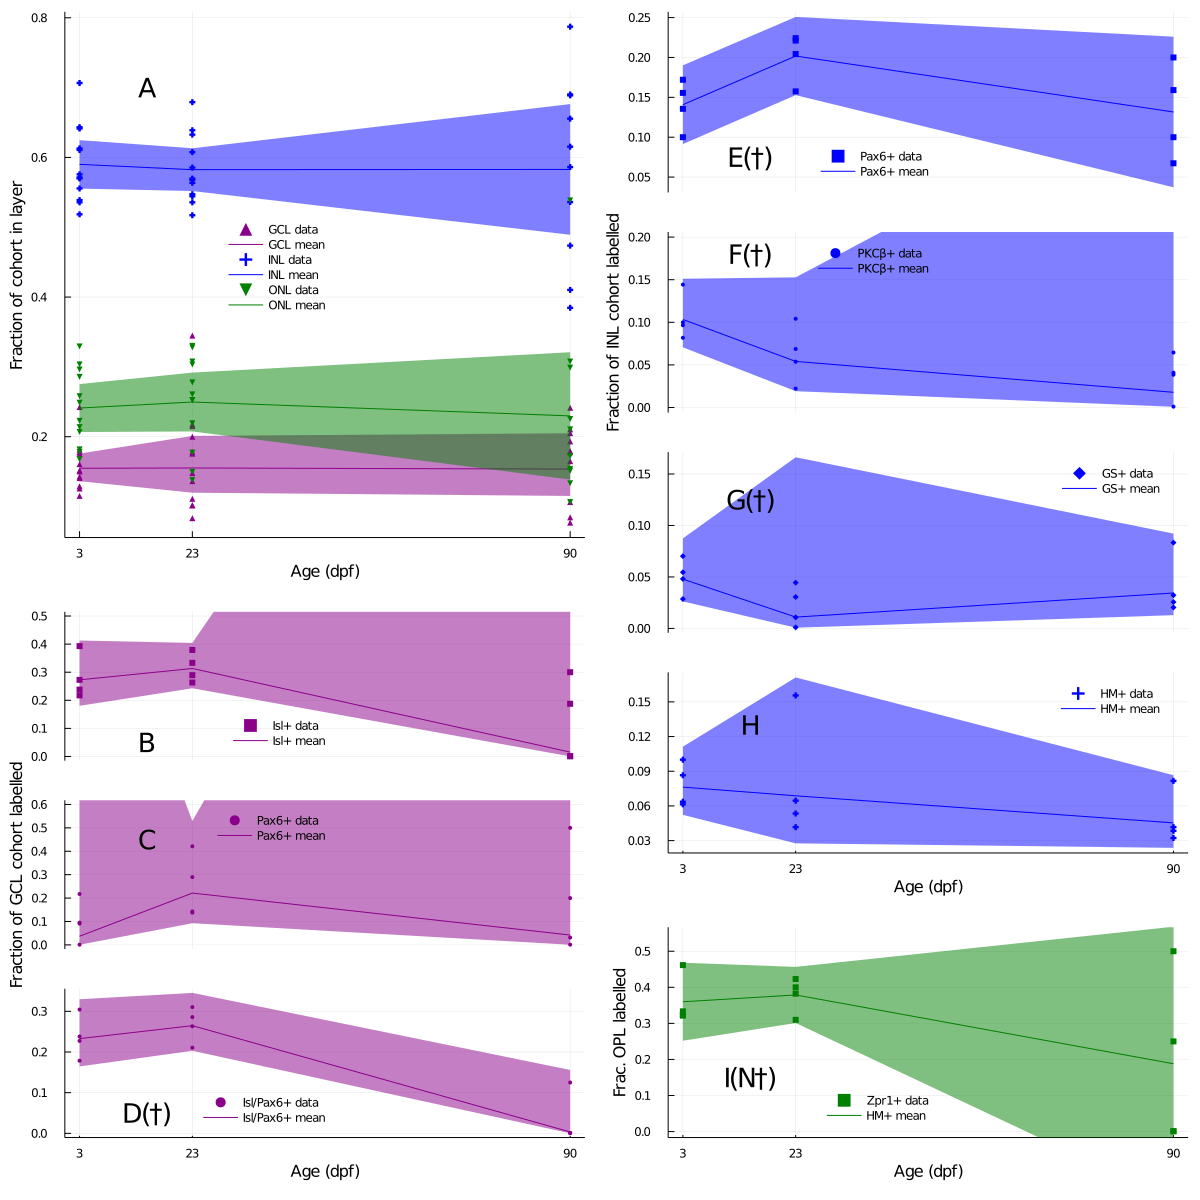
\includegraphics[width=1.2\textwidth]{cmz/layercontributions.png}}    
    \caption{{\bf Second-phase declines in CMZ-contributed Isl\/Pax6+ RGCs, PKC$\beta$+ bipolar neurons, and Zpr1+ double cones}}
    Overall fraction of CMZ-contributed cohort entering cellular layers (Panel A), or fraction of the layer subcohort expressing the noted immunohistochemical marker of lineage. All mean values are presented as marginal posterior means $\pm$ 95\%CI.

    $\lambda$: Fractional lineage contribution is modelled Log-Normally

    $\dagger$: Evidence supports time-varying model of fractional lineage contribution

    Magenta: GCL measurements; Blue: INL measurements; Green: ONL measurements

    Methods in \autoref{ssec:CMZlintrace}, \autoref{ssec:GMCev}.
    Code in \autoref{ssec:a19lineagetrace}.    
    \label{layercontributions}
\end{figure}

These data take the form of fractions of the thymidine-labelled cohort entering each of the three cellular layers (panel A of \autoref{layercontributions}), or the subfraction of the cohort within a given layer expressing a particular cellular marker (Panels B-I). While some variability is apparent in all of the measurements, it is unclear whether it is well-described as time-dependent in most cases. In order to address the question of whether CMZ layer or lineage outcomes differ over time, we needed to assess the joint evidence for separate models of each measurement at each age, against the evidence for a single model of the measurement for all of the assessed ages. 

Because it is not obvious that these fractional measurements are better described Log-Normally, as the underlying population counts are, we first assessed the joint evidence for Normal and Log-Normal models of the data, summarized in Supplementary \autoref{lineage_nlnev}. This supports Log-Normal modelling of all measurements aside from the INL and ONL overall fractions, as well as GCL-resident Pax6- and ONL-resident Zpr1-positive cells. We noted that the evidence estimates differs from the simple likelihood ratio tests in some cases, as summarized in Supplementary \autoref{lineage_lhratio}.  Without a clear fundamental justification for uniformly preferring one model or the other, we selected the best-supported model for each measurement. We estimated the evidence for an age-marginalized model, representing stable contribution to the layer or lineage over time, and compared this to the joint evidence for separate models at each age, representing a time-varying contribution model. These estimates are presented in \autoref{lineage_ev}.

\begin{table}[!ht]
    \caption{{\bf Evidence supports stable layer contributions with time-varying fate commitment}}
    \begin{tabular}{|l|l|l|l|l|l|l|} 
        \hline
        {\bf Layer} & {\bf Marker} & {\bf Cell type} & {\bf Stable logZ} & {\bf Time-vary logZ} & {\bf logZR} & {\bf $\sigma$ sign.}\\ \hline \hline
        GCL & Cohort & All GCL cells & {\bf -0.84 ± 0.71} & -30.96 ± 1.0 & 30.1 ± 1.2 & 24.7\\ \hline \hline
        GCL & Isl2b & RGC & -48.68 ± 0.26 & {\bf -23.76 ± 0.59} & -24.92 ± 0.64 & 39.0\\ \hline
        GCL & Pax6 & Displaced am. & {\bf -23.85 ± 0.44} & -40.08 ± 0.71 & 16.24 ± 0.84 & 19.3\\ \hline
        GCL & Isl2b/Pax6 & RGC subtype & -32.97 ± 0.28 & {\bf -16.82 ± 0.83} & -16.14 ± 0.87 & 18.5\\ \hline \hline
        INL & Cohort & All INL cells & {\bf -41.15 ± 0.49} & -52.65 ± 0.66 & 11.5 ± 0.82 & 14.0\\ \hline \hline
        INL & Pax6 & Amacrine cell & -15.37 ± 0.57 & {\bf -9.14 ± 0.46} & -6.23 ± 0.73 & 8.5\\ \hline
        INL & PKC$\beta$ & Bipolar cell & -5.99 ± 0.3 & {\bf 2.81 ± 0.54} & -8.79 ± 0.62 & 14.2\\ \hline
        INL & GS & M\"{u}ller glia & 14.34 ± 0.35 & {\bf 10.18 ± 0.6} & 4.17 ± 0.7 & 6.0\\ \hline
        INL & HM & Horizontal cell & {\bf 12.0 ± 0.31} &  3.02 ± 0.6 & 8.98 ± 0.68 & 13.3\\ \hline \hline
        ONL & Cohort & All ONL cells & {\bf -47.42 ± 0.45} & -63.19 ± 0.7 & 15.77 ± 0.83 & 19.1\\ \hline \hline
        ONL & Zpr1 & Double cones & {\bf -18.79 ± 0.37} & -31.63 ± 0.6 & 12.84 ± 0.7 & 18.3\\ \hline
    \end{tabular}
    \begin{flushleft}logZ: logarithm of p(D), the marginal likelihood of the data, or model evidence.  Largest evidence values bolded. logZR: evidence ratio; positive values in favour of stable model.
    Methods in \autoref{ssec:CMZlintrace}, \autoref{ssec:GMCev}.
    Code in \autoref{ssec:a19lineagetrace}.    
    \end{flushleft}
    \label{lineage_ev}
\end{table}

These calculations demonstrate that there is evidence for time-varying contributions to the retina, in particular, to RGC, amacrine, bipolar, and M{\"u}ller glial fates. All of these findings have between 6 and 39 standard deviations of significance. In the INL, the trend of the posterior mean for PKC$\beta$-positive bipolar neurons (panel F) and GS-positive M{\"u}ller glia of these lineages declines from the early postembryonic period (3dpf) to the late juvenile period (90dpf). Most of the time-varying fates show a downward trend in the fraction of the cohort expressing the relevant marker. These time-varying, declining lineages may be functionally related. However, we have no specific evidence that would implicate Isl2b/Pax6 double-positive RGCs in circuits with bipolar or amacrine cells, for instance. This nonetheless provides an explanation for the observation of a more-ordered retinal mosaic in later retinal contributions relative to the embryonic central remnant: since one or more sublineages in each layer are depleted in older fish, a different overall mosaic pattern as the neurons associate and pack together is expected. This may occur by changing the pattern of crystalline defects in this packing order, recently suggested as a mode of mosaic organisation \cite{Nunley2019}. Based on the timing of these changes, we tentatively ascribe this differential lineage production to the later phase of CMZ contribution, after the balance between proliferation and niche exit has shifted to the latter.

Lastly, we investigated the possibility that there might be detectable differences in layer or lineage contributions across the dorso-ventral axis; we tested this by measuring the evidence for age-marginalized combined models of fractional contribution against age-marginalized models split along the dorso-ventral axis. We found no evidence to support this hypothesis. These results are presented in Summary \autoref{lineage_dvev}.

\FloatBarrier

\section{Early retinal cohorts of the \textit{D. rerio} retina are turned over at a low rate by 4C4-positive microglia}
\label{sec:neuralfate}
Recently, extensive neural death has been reported in older zebrafish retinae \cite{Vanhoucke2018}. This was described as a ``neurodegenerative pathology" and suggested as a model of age-related neurodegeneration. However, during our thymidine analogue pulse-chase studies, CMZ-contributed cohorts often appeared less numerous only a month or two after their entry into the neural retina, even in juveniles of 30-90 days of age. Moreover, we observed numerous 4C4-positive microglia associating with the CMZ, as displayed in Supplementary \autoref{4C4micrograph}, which suggested that microglia may prune CMZ contributions. If neural retinal turnover occurs throughout the life of the organism, this would belie view that it should be treated as pathological, rather than constitutive. However, the thinning phenomenon could be explained by the changing morphology and geometry of the neural retina during this period. In particular, the neural retina thickens noticeably over this time, as displayed in Supplementary \autoref{morphology}. Although this increase is due, in large part, to the lengthening of photoreceptor outer segments, the inner nuclear layer is also significantly thickened. It is plausible that this process involves a compaction of the neurons along the coronal axis typically sampled, thus appearing to lose cells over time without this actually occurring. 

To investigate, we administered 24 hr pulses of EdU to 1dpf embryos, and followed with 24 hr pulses of BrdU at 23dpf to mark a CMZ-contributed cohort near the height of its activity. By taking both coronal and transverse sections through the eyes of animals at 30, 60, and 90 dpf, we sampled these cohorts from both morphological axes of the retina, and counted labelled sectional totals. Data were totalled across morphological axes to account for the possibility of the cohorts being compacted on the coronal plane and extended on the transverse one. In order to test the hypothesis of early turnover, we estimated the evidence for linearly correlated and uncorrelated models of cohort population over time, using the \hyperref[ssec:EmpiricalBayes]{Empirical Bayes} regression method. If the addition of a time-dependent term in the correlated regression model is justified by the evidence at these early ages, this supports the notion that \textit{D. rerio} retinal turnover is a lifelong phenomenon; if not, the apparent contraction of the cohorts is more likely a function of the alternative explanations noted above, or is occurring at too low a rate to be detected by these means. The results are summarized in \autoref{turnovertable}, with the regressions plotted in Supplementary \autoref{a27linreg}.

\begin{table}[!ht]
    \centering
    \caption{{\bf Evidence for linear regression models supports early cohort population stability}}
    \begin{tabular}{|l|l|l|l|}
    \hline
    {\bf Measurement} & {\bf Stable logZ} & {\bf Declining logZ} & {\bf logZR}\\ \hline
    1dpf Central Remnant & {\bf -212.953} & -214.167 & 1.213\\ \hline    
    30dpf Cohort & {\bf -107.567} & -110.827 & 3.261\\ \hline
    \end{tabular}
   
    \begin{flushleft}logZ: logarithm of p(D), the marginal likelihood of the data, or model evidence.  Largest evidence values bolded. logZR: evidence ratio; positive values in favour of stable model.
    Methods in \autoref{ssec:CMZEdU}, \autoref{ssec:CMZEmpBayes}.
    Code in \autoref{ssec:a27linreg}.
    \end{flushleft}
    \label{turnovertable}
\end{table}

There is more evidence for a model of cohort population that is stable over time than one correlated with time, indicating that the additional model complexity implied by allowing turnover is unjustified, for this early period. Despite this, we did find isolated instances where members of these cohorts were visibly being engulfed by 4C4-positive microglia; one such event is depicted in \autoref{CMZ4C4micrograph}. Moreover, we also observed TUNEL-positive nuclei in the central retina of \textit{rys} siblings in the early postembryonic period (\autoref{caspase}). This indicates that some level of turnover is occuring during this earlier period. The evidence ratio in favour of the uncorrelated models is not overwhelming, which suggests that the cohorts are not turned over at a high enough rate to be detectable in the early period, although the process does occur even at this early age. In order to confirm this finding, we estimated the evidence for age-marginalized Log-Normal models of the population counts against age-differentiated models, representing time-constant and time-varying population models. This investigation resolves any ambiguity: no time-varying model is justified by the available evidence, as summarized in \autoref{turnoverGMCtable}.

\begin{figure}[!h]
    \makebox[\textwidth][c]{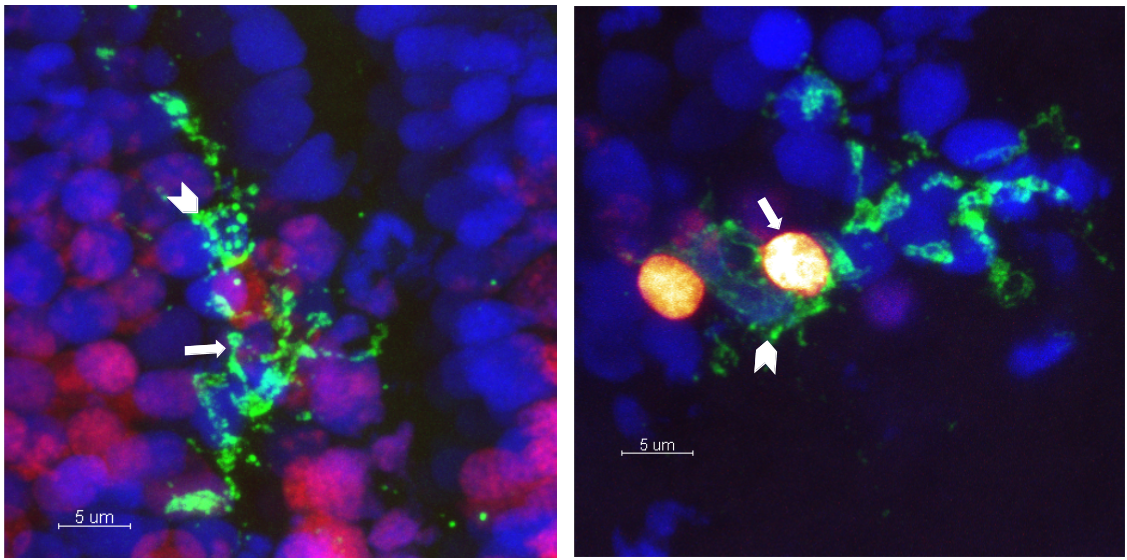
\includegraphics[width=1.\textwidth]{cmz/4C4engulfment.png}}    
    \caption{{\bf 4C4+ microglia associate with and engulf EdU-labelled CMZ contributions in the specified neural retina}}
    Representative maximum intensity projections from confocal micrographs of 14\si{\micro\metre} coronal cryosections through 30dpf zebrafish eyes labelled at 23dpf with EdU.
    
    Blue: Hoechst 33258 nuclear counterstain. Green: Microglia labelled with 4C4 antibody. Red-orange-yellow: Intensity scale of EdU staining, indicating cellular origin in the 23dpf CMZ.

    Chevrons: microglial nuclei. Arrows: EdU-positive nuclei found within 4C4-labelled extent of microglial cell body and appendages.
    
    Methods in \autoref{ssec:CMZ4C4histo}.
    \label{CMZ4C4micrograph}
\end{figure}

\begin{table}[!ht]
    \centering
    \caption{{\bf GMC-NS evidence estimates confirm Empirical Bayes analysis of early cohort stability}}
    \begin{tabular}{|l|l|l|l|l|} \hline 
        {\bf Cohort} & {\bf Time-constant logZ} & {\bf Time-varying logZ} & {\bf logZR} & {\bf $\sigma$ Significance}\\ \hline
        Embryonic central remnant & {\bf -857.08 ± 0.29} & -868.02 ± 0.6 & 10.94 ± 0.67 & 16.4\\ \hline
        1 month CMZ & {\bf -402.38 ± 0.31} & -405.76 ± 0.43 & 3.39 ± 0.53 & 6.4\\ \hline
    \end{tabular}
    \begin{flushleft} logZ: logarithm of p(D), the marginal likelihood of the data, or model evidence. logZR: evidence ratio; positive ratios in favour of the 2-phase model. Largest evidence value bolded.
    Methods in \autoref{ssec:CMZEdU}, \autoref{ssec:GMCev}.
    Code in \autoref{ssec:a27GMC_NS}.
    \end{flushleft}
    \label{turnoverGMCtable}
\end{table}

\section{Summary: Modelling the postembryonic CMZ}
CMZ population dynamics, as encapsulated in our datasets, are best explained by a model of slowly decaying cell cycle rate and constant niche exit rate. This parameterisation is superior to phased models of CMZ activity, although both imply an initial period characterised by CMZ population growth, followed by a second phase of during which the CMZ is depleted. These dynamics can be achieved with a a wide range of cycle times and niche exit rates, which we show by establishing posterior distributions on these parameters. These demonstrate that our estimates of cell cycle lengths are better constrained by our data than estimates of exit rates. The population of the CMZ displays an asymmetric structure which reverses over time; we have shown this is not due to time-shifting of the two proliferative phases across anatomical axes, nor can it be explained by different initial cell cycle times and decay rates. The proportional layer composition of CMZ-driven contributions is stable over this time, and does not display variability over the dorso-ventral axis. However, by estimating the evidence for time-stable and time-varying models of lineage contribution, we identified a decline in particular retinal lineage subtypes, particularly those of the INL, but including the GCL. This a potential explanation for the teleost postembryonic change in retinal mosaic pattern. Finally, we have shown that microglia-mediated turnover of retinal neurons is occurring at a rate too low to have a measurable effect on cohort sizes during this time.

Thus, the niche history of the CMZ is not adequately explained by a ``frozen'' population of RPC progenitors, homeostatically recapitulating a program of development found in embryonic progenitors, as has been suggested previously \cite{Harris1998,Wan2016}, for the proliferative potential implied by these models is too low. Instead, a model that does not limit the size of lineages, but has a slowly decaying cell cycle rate, is sufficient to produce the observed niche population history. This suggests that the postembryonic CMZ is under a separate regulatory regime from the embryonic RPCs, which contribute the central, larval remnant of the neural retina. This period of RPC activity benefits from separate modelling and investigation. Moreover, the decaying cycle rate model suggests an explanation for the difference between animals that have sustained CMZ RPC activity in adulthood, like teleosts, versus those that do not, such as mammals: the rate of decay in mammals may simply be much higher.

In addition to discovering unique features of postembryonic CMZ activity, we have proved out a general framework for Bayesian evaluation and selection of arbitrary biological models, which can inform both future experiments as well as modelling and theoretical choices. For instance, slice models more successfully combine population and morphological information, to answer questions about CMZ population structure, than do abstract whole-population models of the CMZ. From the foregoing analyses, we conclude that treating the CMZ population as a combined unit with shared proliferative parameter evolution is likely well justified, suggesting that much of the apparent complexity of the niche's population history can be usefully abstracted away.

\section{Future directions}
These studies show that the simple datasets we have collected are sufficient to suggest a general model of the postembryonic CMZ, which does not explicitly limit the proliferative potential of RPCs by a measure of time in lineage, like the SMME models. However, they also reveal that these datasets provide little constraint on many important parameters of interest. This is an important insight, as future experiments can be designed with the nested sampling model comparison in mind. For instance, our models consistently exhibit poorly constrained niche exit rates. The kinetics of niche exit could be examined by thymidine pulse-chase assays, timed to catch cohorts of RPC progeny as they cross the boundary from the CMZ into the neural retina, and this would likely significantly improve our estimates. Cell-based models of cycle parameters can glean some information from cumulative thymidine analogue labelling alone, but these would be greatly improved with costaining for markers of other cycle phases, for instance using phosphorylated histone H3 as a marker of M phase \cite{Ren2018}. Experiments using multiple different thymidine analogue labels \cite{Harris2018} are another avenue for refining these estimates.

In general, the model comparison approach worked out here seems promising for testing competing explanations for observed phenomena. It would be worthwhile to improve the accuracy of \hyperref[chap:GMC]{\path{GMC_NS.jl}}, and to continue developing models that make reference to the widest available array of observations and interventions. Given some adjustments to the experimental approach, and a refined sampler, this approach could replace obsolete models of cell cycle like the one described by Nowakowski et al. \cite{Nowakowski1989}, while giving a more realistic picture of the information actually provided by particular datasets.

As a final remark, it should be emphasized that the conclusions of this chapter always refer to the quality distribution jointly implied by the model and the data. Despite our failure to distinguish between RPC behaviours in different morphological regions of the CMZ, these rejected hypotheses should be returned to and re-tested with refined models and datasets. The same is true of phased and single-regime models of RPC cell cycle regulation. By proceeding in this manner, as Feyerabend suggested, we can ``maximise the empirical content of [our] views" by ``try[ing] to improve rather than discard the views that have failed in the competition.'' \cite[p.20]{Feyerabend1993}
\chapter{Mutant npat results in nucleosome positioning defects in \textit{D. rerio} CMZ progenitors, blocking specification but not proliferation}
\chaptermark{Nucleosome position and specification defects in npat mutant \textit{rys}}
\label{chap:rys}
\section{Introduction}
The zebrafish (D. rerio) circumferential marginal zone (CMZ), located in the retinal periphery, contains the retinal stem cells and progenitors responsible for the lifelong retinal neurogenesis observed in this cyprinid. Analagous to CMZs in other model organisms, such as X. laevis \cite{Perron1998}, it has been of particular interest to us since the discovery of quiescent stem cells at the mammalian retinal periphery \cite{Tropepe2000}, as an understanding of the molecular mechanisms regulating this proliferative zone may shed light on whether these mammalian cells might be harnessed for the purpose of regenerative retinal medicine. While significant progress has been made in this direction \cite{Raymond2006}, molecular lesions in a plethora of zebrafish mutants displaying defects in CMZ development and activity remain largely uncharacterised. We examine here one such micropthalmic line identified in an ENU screen, \textit{rys} \cite{Wehman2005}, characterised by Wehman et al. as a Class IIA CMZ mutant, with a small eyes (see \autoref{ryspic}) and apparently paradoxically enlarged CMZ.

\begin{figure}[!h]
    \makebox[\textwidth][c]{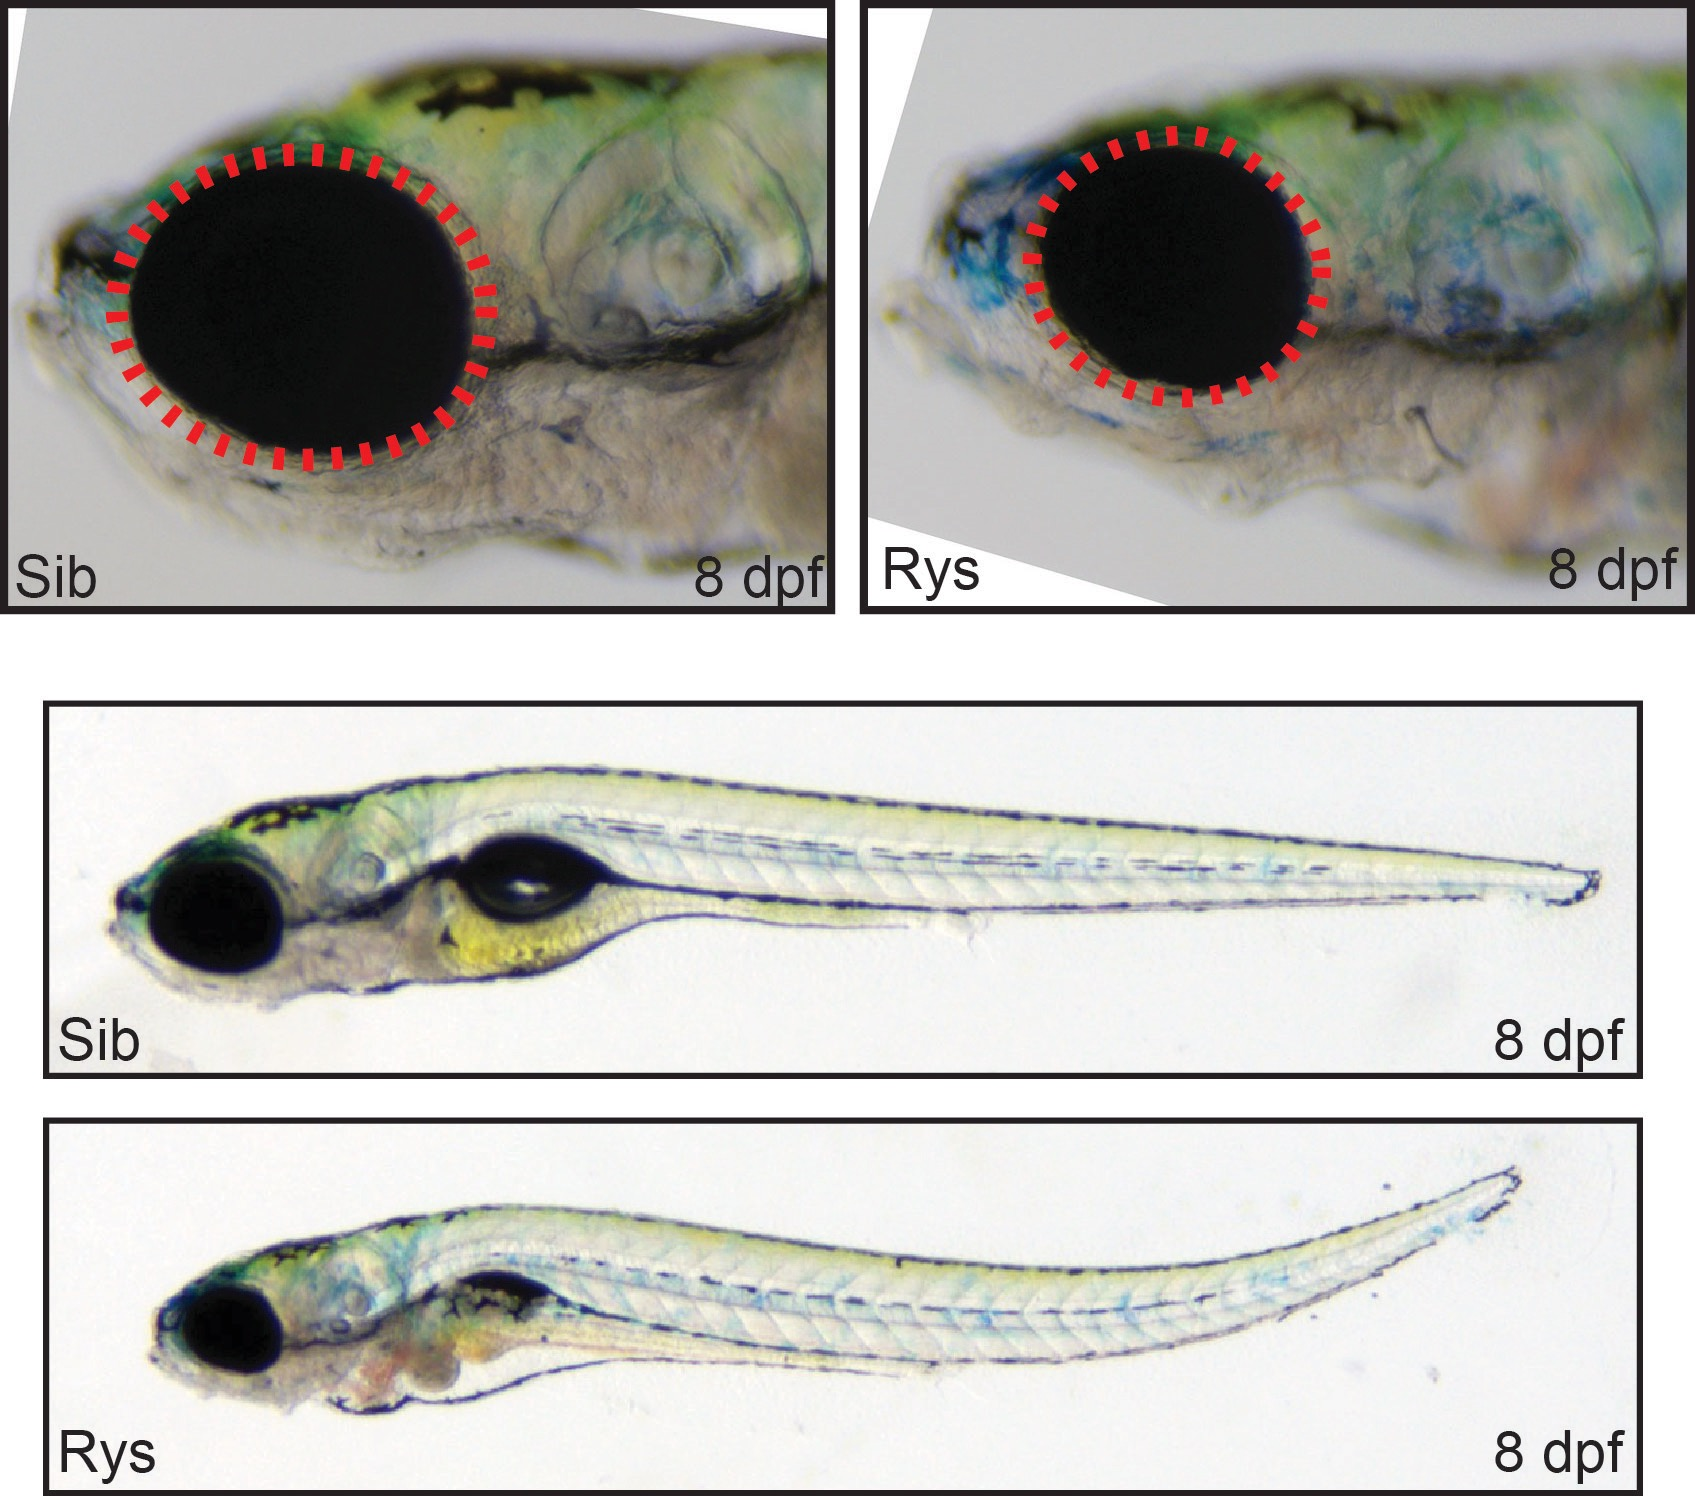
\includegraphics[width=.6\textwidth]{rys/rys.jpg}}    
    \caption{{\bf \textit{rys} mutants exhibit a small-eye phenotype}}
    \label{ryspic}
    8 dpf \textit{rys} sibling (Sib) and mutant (Rys), head area (top panels), whole body (bottom panels). Red dashes highlight the overall reduced eye size in homozygous \textit{rys} mutant animals.
\end{figure}

Mapping revealed the causative \textit{rys} mutation lay in the zebrafish npat gene, the nuclear protein associated with the ataxia-telangiectasia locus in mammals \cite{Imai1996}. Although npat is heretofore uncharacterised in zebrafish, its mammalian homologues, human NPAT and mouse Npat, have been extensively examined. These studies have demonstrated that NPAT plays a critical role in coordinating events associated with the G1/S phase transition in proliferating cells \cite{Ye2003}. S-phase entry requires tight co-ordination between the onset of genomic DNA synthesis and histone production, in order to achieve normal chromatin packaging and assembly. NPAT, found in the nucleus \cite{Sagara2002} and localised, in a cell-cycle dependent manner, to histone locus bodies \cite{Ghule2009}, induces S-phase entry \cite{Zhao1998} and activates replication-dependent histone gene transcription by direct interaction with histone gene clusters \cite{Zhao2000} in association with histone nuclear factor P (HiNF-P) \cite{Mitra2003}. The protein’s effects on S-phase entry and histone transcription are associated with distinct domains at the C-terminus and N-terminus, respectively \cite{Wei2003}. NPAT is also known to associate with the histone acetyltransferase CBP/p300 \cite{Wang2004} and directs histone acetylation by this enzyme \cite{He2011}.

NPAT is known to be a component of the E2F transcriptional program \cite{Gao2003} and a substrate of cyclin E/CDK2 \cite{Zhao1998}, although E2F-independent activation by cyclin D2/CDK4 in human ES cells has also been described \cite{Becker2010}. The expression of NPAT protein peaks at the G1/S boundary \cite{Zhao1998}, as does its phosphorylation, which promotes its transcriptional activation of replication-dependent H2B \cite{Ma2000} and H4 \cite{Mitra2009} genes, while its effect on low, basal levels of H4 transcription is phosphorylation-independent \cite{Ye2003}. Of particular interest, NPAT has recently been found to be required for CDK9 recruitment to replication-dependent histone genes \cite{Pirngruber2010}; CDK9 and monoubiquitinated H2B are essential for proper 3’ end processing of stem-loop histone transcripts \cite{Pirngruber2009}. NPAT and HiNF-P have also been found associated with the U7 snRNP complexes that perform this function \cite{Ghule2009}. The replication-dependent activities of NPAT are thought to be terminated by WEE1 phosphorylation of H2B, which excludes NPAT from histone clusters \cite{Mahajan2012}.

All of these studies have been conducted in tissue culture contexts, perhaps due to the challenges associated with studying this critical protein in vivo; mouse embryos with provirally inactivated Npat arrest at the 8-cell stage, for instance \cite{DiFruscio1997}. The availability of \textit{rys}, a zebrafish npat mutant which develops well into the larval stage, is therefore of considerable interest, as it allows for the study of npat’s function within complete tissues. We demonstrate here that npat is critical for the normal proliferation and differentiation of CMZ neural progenitors.

We find substantial evidence for the role of \textit{D. rerio} npat involvement with histone transcription, nucleosome positioning, and scheduling of mitotic activity; we suggest that the \textit{rys} phenotype is brought about by a failure to coordinate the genomic states required to specify, independently of proliferative capacity, in postembryonic zebrafish RPCs of the CMZ.

\section{Results}
\subsection{The \textit{rys} CMZ phenotype is characterised failure of RPCs to specify, altered nuclear morphology, aberrant proliferation and expanded early progenitor identity}

\textit{rys} has previously been described as having an enlarged CMZ \cite{Wehman2005}, but whether this is a consequence of an enlarged proliferative population, altered cellular morphology, or other causes, remained unclear. We sought to learn more about the ontogeny of the mutant niche by examining two histochemical markers of cycle activity during the early life of \textit{rys}; Proliferating Cell Nuclear Antigen (PCNA), which in \textit{D. rerio} is expressed throughout the cell cycle, and the genomic incorporation of the thymidine analogue EdU over a 24 hour pulse, which indelibly marks cells that have passed through S-phase whilst exposed to it. These data are displayed in \autoref{rysCMZontogeny}. During this period, the PCNA positive population of the sibling CMZ declines precipitously (Panel A), with a corresponding decrease in proliferative activity as measured by the incorporation of EdU (Panel B). Whether or not the \textit{rys} CMZ population is enlarged by comparison depends on the age at which it is sampled, with there is a 99.6\% probability of the posterior mean sectional \textit{rys} CMZ PCNA population being below the sib mean at 4dpf, while 99.8\% of the marginal posterior of the 10dpf \textit{rys} mean lies above that of sibs. Therefore, the \textit{rys} CMZ population is better described as achieving its peak periembryonic size later than siblings; its population is only numerically larger than sibs at later ages\footnote{\textit{rys} animals universally die by approximately 3 weeks of age.}. 

\begin{figure}[!h]
    \makebox[\textwidth][c]{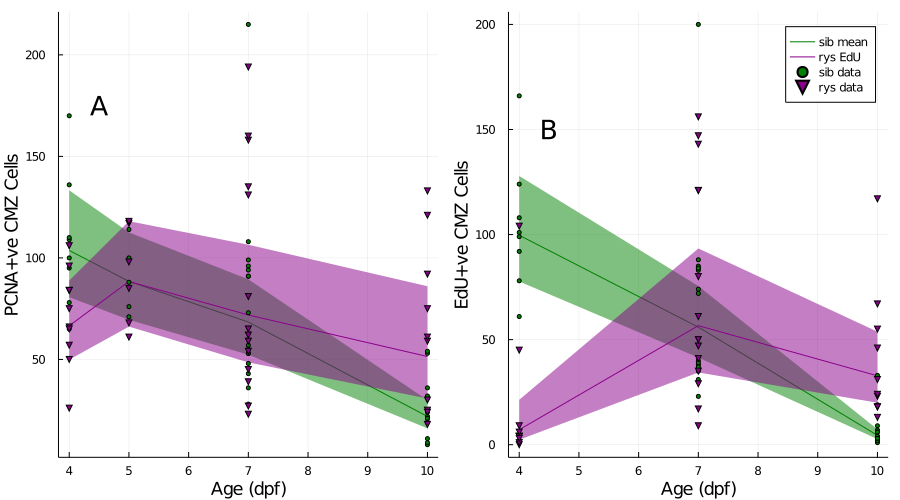
\includegraphics[width=1.\textwidth]{rys/CMZontogeny.png}}    
    \caption{{\bf \textit{rys} CMZ populations start relatively small and quiescent, end abberantly large and proliferative}}
    Panel A: Counts and estimated mean $\pm$95\% credible intervals of PCNA-positive cells in the peripheral CMZ of \textit{rys} (magenta) and their siblings (green)
    Panel B: As above, but for counts of double PCNA-,EdU-positive cells in the CMZ after a 24 hour pulse of EdU.
    \label{rysCMZontogeny}

\end{figure}
\FloatBarrier

Surprisingly, very few \textit{rys} animals have many actively cycling RPCs at 4dpf, by comparison to the robustly cycling sib RPCs at this age; a mean estimate of 96.2$\pm$3.4\% of sib RPCs are labelled during the 24 hr pulse at 4dpf, while only 24.1$\pm$37.2\% of \textit{rys} RPCs are. The situation is broadly reversed at 10dpf, with only 24.4$\pm$14.9\% of sib RPCs labelled, compared to 65.8$\pm$16.2\% of \textit{rys} RPCs. While we questioned whether this late-stage increase in \textit{rys} thymidine analogue labelling might not represent bona fide mitotic activity, we were able to readily find mitotic figures within these populations, shown in Supplementary \autoref{rysmitosis}. As the data convey, these outcomes are highly variable in both sib and \textit{rys} animals, with, for instance, an isolated mutant at 4dpf sporting an EdU-positive population near the sibling mean. However, even in those \textit{rys} animals which do have actively proliferating RPCs at these earlier ages, there is a marked failure of the CMZ to contribute to the postmitotic, specified neural retina. Confocal micrographs displaying \textit{rys} CMZ cohorts labelled with BrdU at 3dpf that have failed to enter the neural retina after 7 days of chase time are displayed alongside their normal siblings in \autoref{contributionfailure}. 

\begin{figure}[!h]
    \makebox[\textwidth][c]{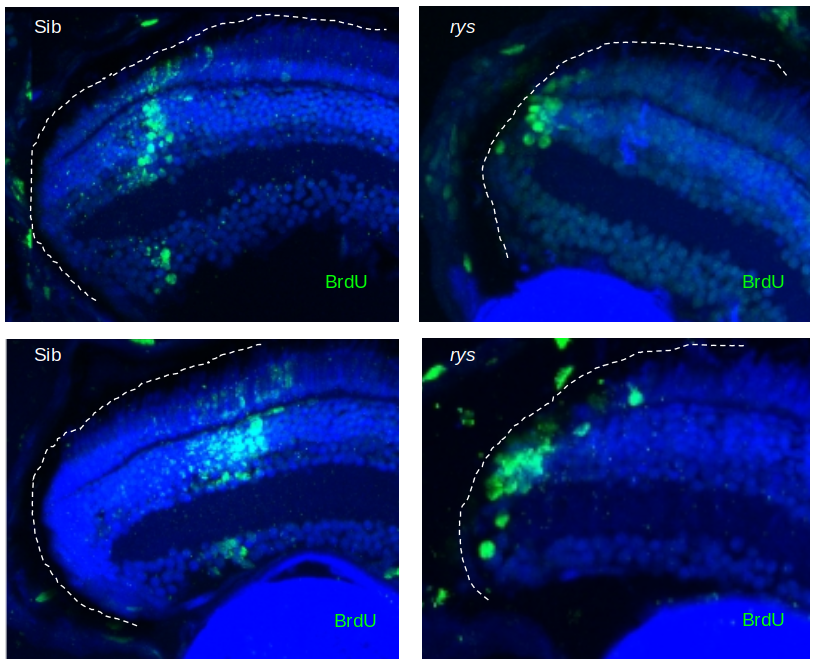
\includegraphics[width=1.\textwidth]{rys/cmzfailure.png}}    
    \caption{{\bf \textit{rys} CMZ RPCs fail to contribute to the neural retina}} M
    14\si{\micro\metre} coronal cryosections through representative sib (left panels) and \textit{rys} eyes at 10dpf, 7 days after an 8hr BrdU pulse at 3dpf. Note that few labelled \textit{rys} cells have entered the specified retinal layers.
    \label{contributionfailure}
\end{figure}
\FloatBarrier

Indeed, a close study of the 5dpf retinae, held back from EdU processing to preserve their nuclear features (presented in \autoref{nuclearstudy}), suggests that the primary reason for the enlarged appearance of \textit{rys} CMZs, even at this age, when the niche's population is numerically similar to siblings (Panel A), is this failure to contribute to the neural retina, leading to \textit{rys} central retinae that are about half as populous, per cell of the CMZ, as their siblings (Panel B). This appearance may be enhanced in the dorsal CMZ, there is an  87.8\% probability that the posterior mean for this region in \textit{rys} is above the sibling mean, although this is compensated for by 97.5\% of the marginal posterior distribution on the ventral mean laying below the same sibling mean (Panels C and D). More significantly, \textit{rys} nuclei tend to be much larger than their siblings (Panel E), as well as consistently less spherical (Panel F).

\begin{figure}[!h]
    \makebox[\textwidth][c]{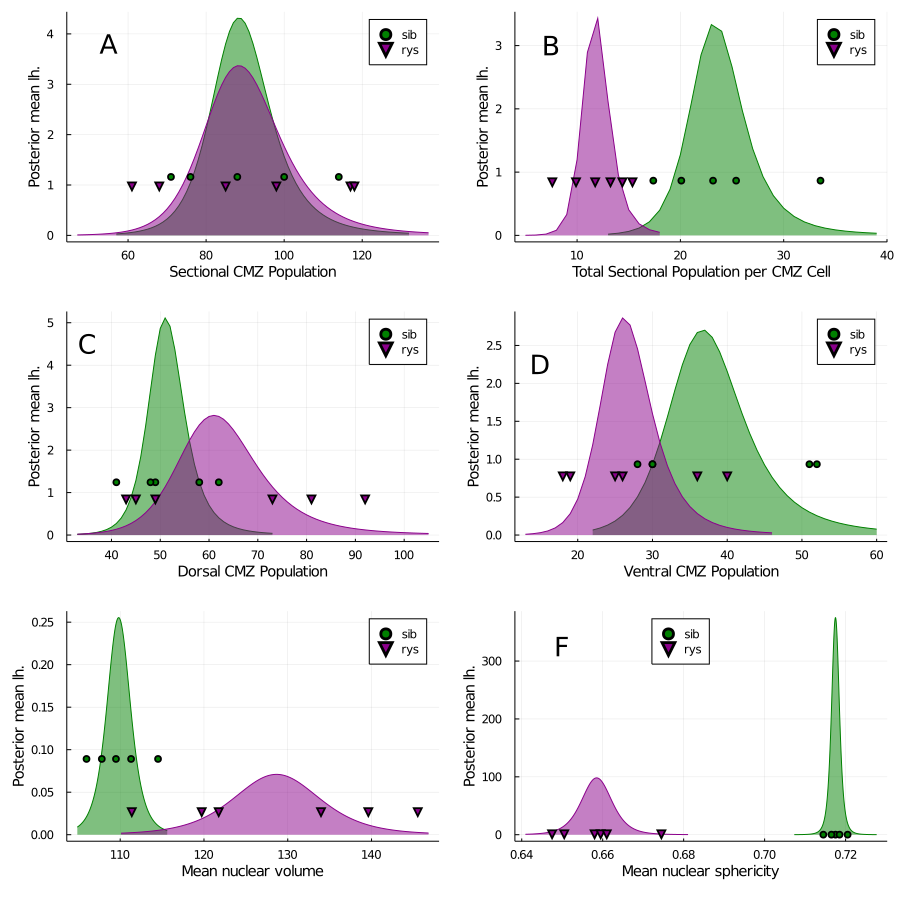
\includegraphics[width=1.\textwidth]{rys/nuclearstudy.png}}    
    \caption{{\bf 7dpf \textit{rys} CMZ RPCs display enhanced asymmetry, increased volume, decreased sphericity, and relative but not absolute enlargement}}
    \label{nuclearstudy}
    All panels display sib observations as green circles and \textit{rys} as magenta triangles. Plotted behind the underlying observations are the calculated marginal posterior distributions of the mean, given log-Normal models of the population data and Normal models of the volume and sphericity data. The y-axis shows the relative likelihood of underlying mean values on the x-axis, given the data.
    Panel A: Total dorsal + ventral CMZ population per central coronal section.
    Panel B: Number of PCNA negative, specified central retinal neurons per PCNA postive CMZ cell.
    Panels C and D: Dorsal and Ventral CMZ populations per central coronal cryosection.
    Panel E: Mean volume of nuclei in a given individual's central coronal cryosection.
    Panel F: Mean sphericity of nuclei in a given individual's central coronal cryosection.
\end{figure}

In order to quantitiatively rank these contributions to the \textit{rys} nuclear phenotype, we calculated the evidence for combined LogNormal (population measurements) and Normal (nuclear measurements) models of sib and rys data, against the joint evidence for separate models. These estimates are presented in \autoref{nuclearev}. Our measurements indicate that the best evidentiated contributors to the \textit{rys} CMZ phenotype are, first, the decrease of nuclear sphericity, followed by the decreased number of central retinal neurons relative to the CMZ, then, the increase in nuclear volume, and lastly the expansion of the dorsal CMZ. These calculations also demonstrate that there is no evidence for overall differences in sectional CMZ population, and that the ventral CMZ is less populous in \textit{rys}, which may contribute to the appearance of an enlarged dorsal CMZ. The large size of the nuclear morphological changes and the decreased number of central cells indicates that these are the most important contributors to the \textit{rys} phenotype.

\begin{table}[!ht]
    \centering
    \caption{{\bf Evidence-based ranking of phenomenal contributors to \textit{rys} phenotype}}
    \begin{tabular}{|l|l|l|l|l|} 
        \hline {\bf Parameter} & {\bf Separate logZ} & {\bf Combined logZ} & {\bf logZR} & {\bf $\sigma$ sign.}\\ \hline 
        Sectional CMZ pop. & -280.8 ± 1.7 & {\bf -183.44 ± 0.9} & -97.4 ± 1.9 & 50.7 \\ \hline
        Central pop./CMZ cell & {\bf -62.51 ± 0.64} & -89.88 ± 0.12 & 27.38 ± 0.66 & 41.7 \\ \hline
        Dorsal CMZ pop.  & {\bf -180.1 ± 1.0} & -192.8 ± 1.1 & 12.8 ± 1.5 & 8.3 \\ \hline
        Ventral CMZ pop. & {\bf -136.86 ± 0.32} & -147.36 ± 0.46 & 10.5 ± 0.56 & 18.8 \\ \hline
        Nuclear Volume & {\bf -164.18 ± 0.29} & -229.3 ± 1.9 & 65.1 ± 1.9 & 34.4 \\ \hline
        Nuclear Sphericity & {\bf -89.1 ± 1.8} & -311.2 ± 3.9 & 222.0 ± 4.2 & 52.3 \\ \hline
    \end{tabular}
    \label{nuclearev}
\end{table}


\FloatBarrier

\begin{figure}[!h]
    \makebox[\textwidth][c]{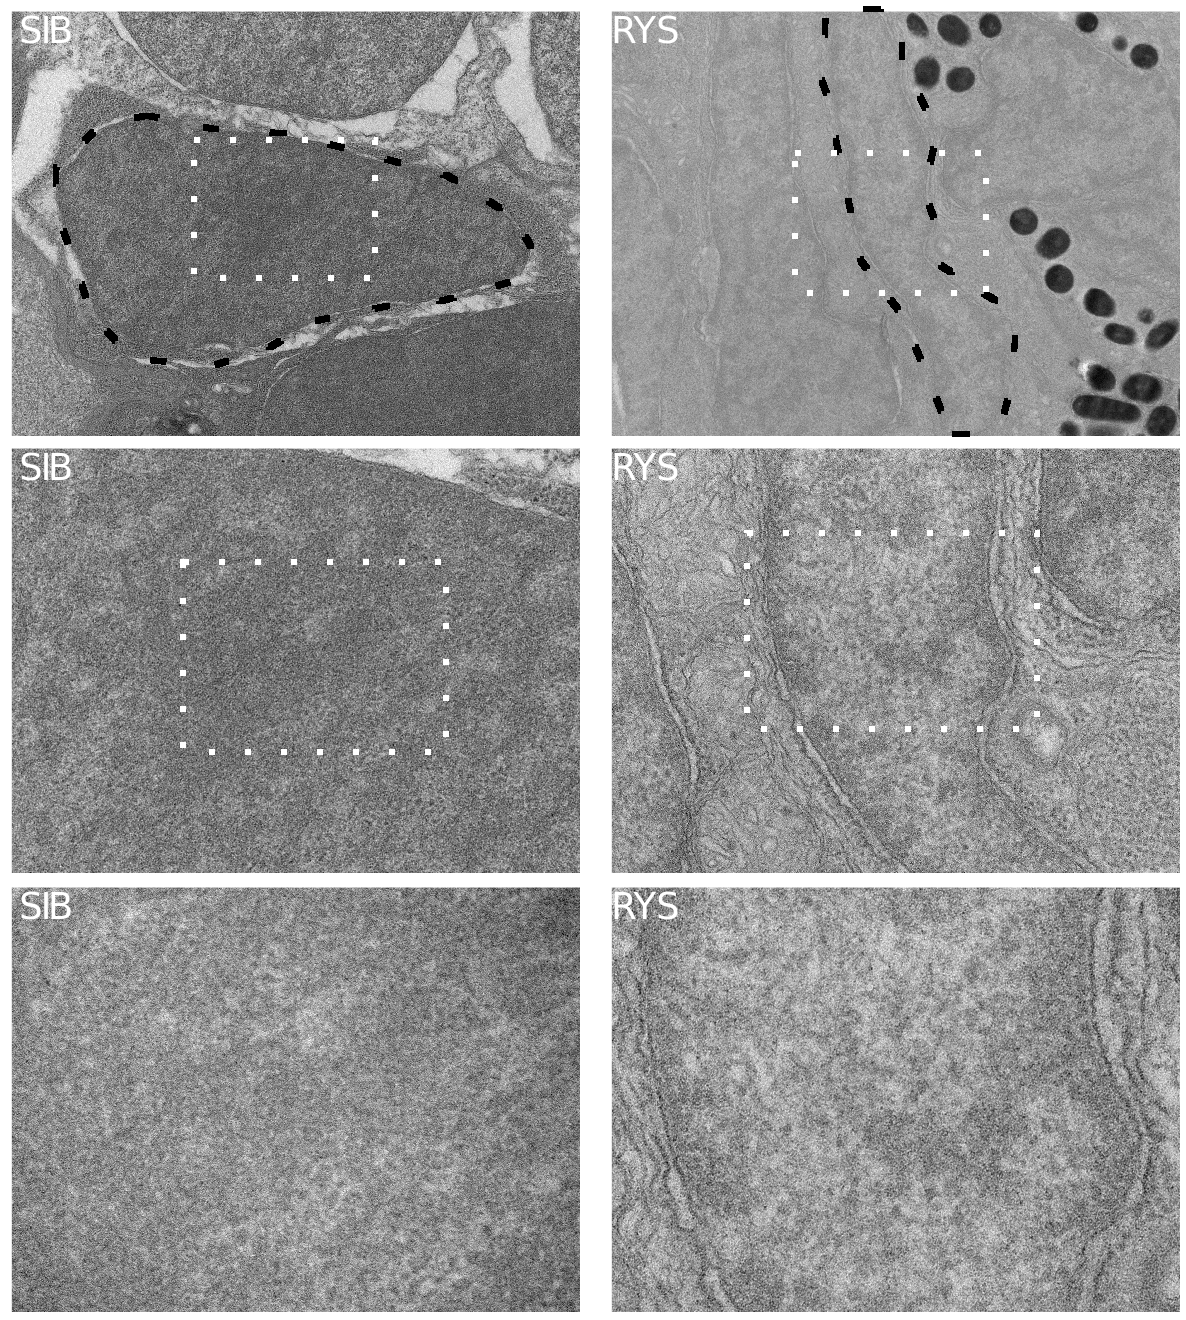
\includegraphics[width=.8\textwidth]{rys/rysem.png}}    
    \caption{{\bf RPC nuclei of the \textit{rys} CMZ display disorganized, loosely packed chromatin}}
    Representative electron micrographs of \textit{rys} sibling and mutant CMZ RPC nuclei.
    Left panels: siblings. Right panels: \textit{rys}. Top panels: 36000x magnification, general overview of the area around the nucleus, dashed black. Area displayed in middle panels dashed white. Middle panels: 110000x magnification nuclear detail. Area displayed in bottom panels dashed white. Bottom panels: 210000x magnification, chromosomal ultrastructure.
    \label{rysEM}
\end{figure}

The characteristically enlarged nuclei in \textit{rys} have a billowy appearance suggestive of chromosomal disorganization. In order to investigate this possibility further, we used electron microscopy to examine the nuclear ultrastructure of RPC nuclei in \textit{rys} and sibling CMZs. Representative electron micrographs are presented in \autoref{rysEM}. At 36000x magnification, the unusual and disorganized structure of \textit{rys} nuclei become apparent, particularly in contrast with the consistently teardrop-shaped nuclei of sibling RPCs; the \textit{rys} nucleus pictured is so pancaked it extends out of the frame that readily captures a sibling nucleus. When the chromatin itself is imaged at 210000x magnification, it appears much less electron-dense in the rys, with much larger tracts of presumptive euchromatin, and less regular spacing of chromosomal material.
\FloatBarrier

If RPCs in \textit{rys} CMZs are failing to enter the specified neural retina, but by 7dpf are becoming mitotically active, this leaves the question of why this apparently proliferative niche's population is declining by 10dpf. We suspected that \textit{rys} RPCs may be undergoing apoptosis in situ. Although we did not detect pyknotic nuclear fragments in our EM investigations, it is possible that the individual apoptotic events are too rare in \textit{rys} to reliably detect in this manner. In order to investigate this possibility, we assayed the presence of caspase-3 in \textit{rys} and sib CMZs. As displayed in \autoref{caspase}, caspase-3-positive nuclei can be detected in the \textit{rys} CMZ at both 4 and 6 dpf (mean 6.5 $\pm$ 7.5 and 2.6 $\pm$ 1.1 cells, respectively) but are not found in sib CMZs, though both display a similar level of central apoptotic activity (4dpf \textit{rys}: 1.25 $\pm$ 1.0; 4dpf sib: 1.4 $\pm$ 1.1; 6dpf \textit{rys} 0.6 $\pm$ 0.9; 6dpf sib: 1.0 $\pm$ 1.4 ). The lack of debris observable in \textit{rys} CMZs is likely attributable to the activity of 4C4-positive microglia active in the area; we observed one such cell actively phagocytosing TUNEL-labelled \textit{rys} RPC nuclear fragments in the CMZ, displayed in Supplementary \autoref{phagocytosis}.

\begin{figure}[!h]
    \makebox[\textwidth][c]{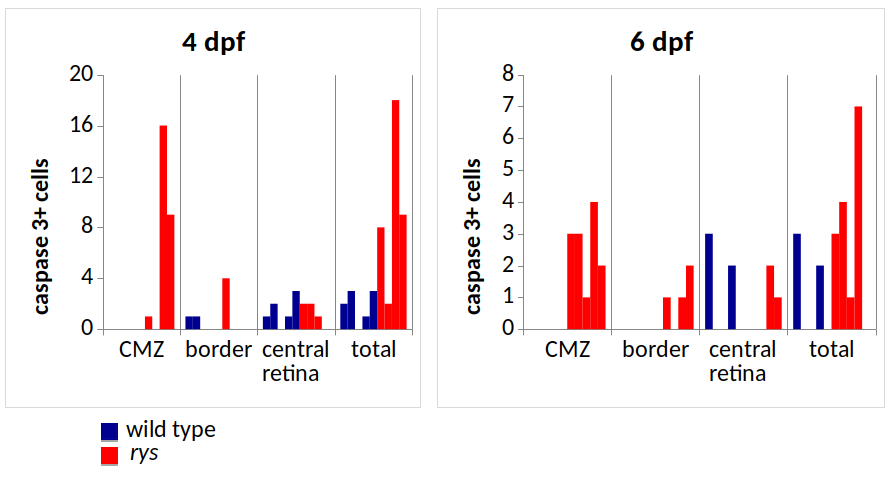
\includegraphics[width=1.\textwidth]{rys/caspase.png}}    
    \caption{{\bf \textit{rys} mutant CMZs have increased caspase-3 positive nuclei}}
    Number of caspase-3 positive cells counted in CMZ, the border between the CMZ and specified central retina, the specified central neural retina, and the overall total, at 4 dpf (left panel) and 6 dpf (right panel). One central \SI{20}{\micro\metre} section per sibling (S) and \textit{rys} (R) larva.
    \label{caspase}
\end{figure}

Suspecting that \textit{rys} CMZ RPCs may maintain an early progenitor identity, causing their failure to contribute to the specified neural retina, we examined pax6a immunostaining of this population, which is normally restricted to putative progenitors in the peripheral and middle CMZ, as well as the retinal ganglion cell layer \cite{Raymond2006}. The Pax6-stained region was enlarged in \textit{rys} CMZs relative to their siblings (\autoref{progenitoridentity}, center panels). As vsx2 is also known to be a marker of retinal progenitor cells in the CMZ \cite{Raymond2006}, we also generated a transgenic vsx2::eGFP \textit{rys} line using a fragment of the zebrafish vsx2 promoter which drives eGFP expression in the utmost retinal periphery in siblings. Mutant fish from this line displayed substantially expanded eGFP expression in the CMZ (\autoref{progenitoridentity}, right panels).

\begin{figure}[!h]
    \makebox[\textwidth][c]{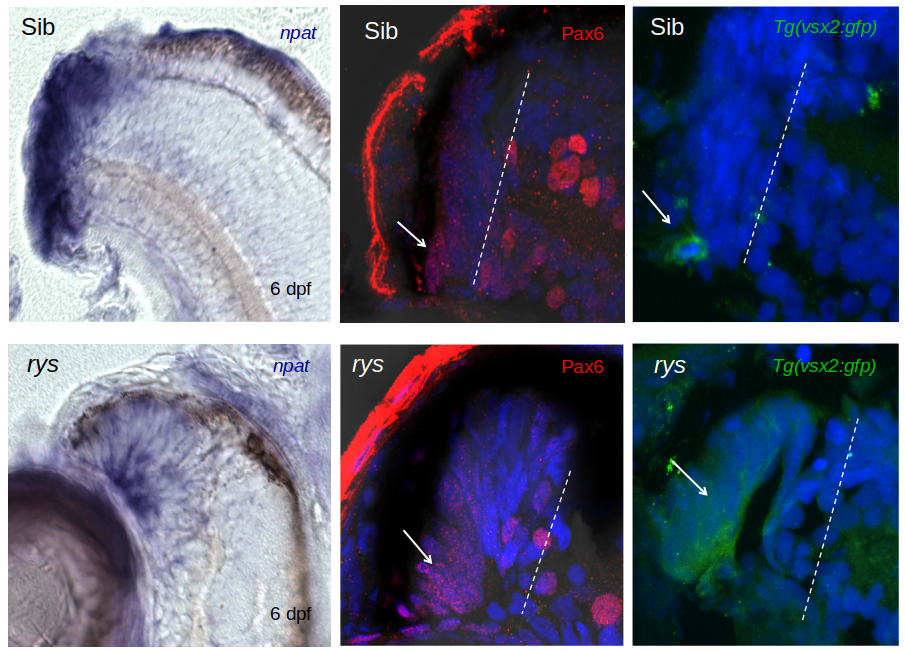
\includegraphics[width=1.2\textwidth]{rys/progenitorid.png}}    
    \caption{{\bf Mutant \textit{rys} RPCs display expanded expression of early progenitor markers}}
    Representative transmitted light and confocal micrographs of \textit{rys} sibling and mutant CMZ RPCs. Top panels: siblings. Bottom panels: \textit{rys} mutants. Left panels: in-situ hybridization using npat probe on 20\si{\micro\metre} coronal cryosection. Middle panels: anti-Pax6 immunohistochemistry. Right panels: GFP expression in a Tg(vsx2:GFP) line introgressed into \textit{rys}. 
    \label{progenitoridentity}
\end{figure}

\FloatBarrier
\subsection{The micropthalmic zebrafish line \textit{rys} is an npat mutant}

In order to determine the causative mutation responsible for the \textit{rys} phenotype, we performed linkage mapping to identify candidate genes, followed by PCR analysis of the transcript products of these candidates. This study revealed a single G\textgreater{}A transition at position 24862961 on chromosome 15 (NC\_007126.5, Zv9), annotated as the first base of intron 9 in the zebrafish npat gene, in a canonical GU splice donor site. 

We observed that this mutation reliably results in the retention of npat intron 8, and less frequently, in the retention of both introns 8 and 11, in 6dpf \textit{rys} mutants, shown in \autoref{npattranscript}. The predicted protein sequence expressed from the mutant transcript is truncated by a stop codon at residue 283, which would preclude the translation of predicted phosphorylation sites and nuclear localisation signals cognate to those identified in human NPAT \cite{Ma2000,Sagara2002}, as displayed in \autoref{npatprotein}.

\begin{figure}[!h]
    \makebox[\textwidth][c]{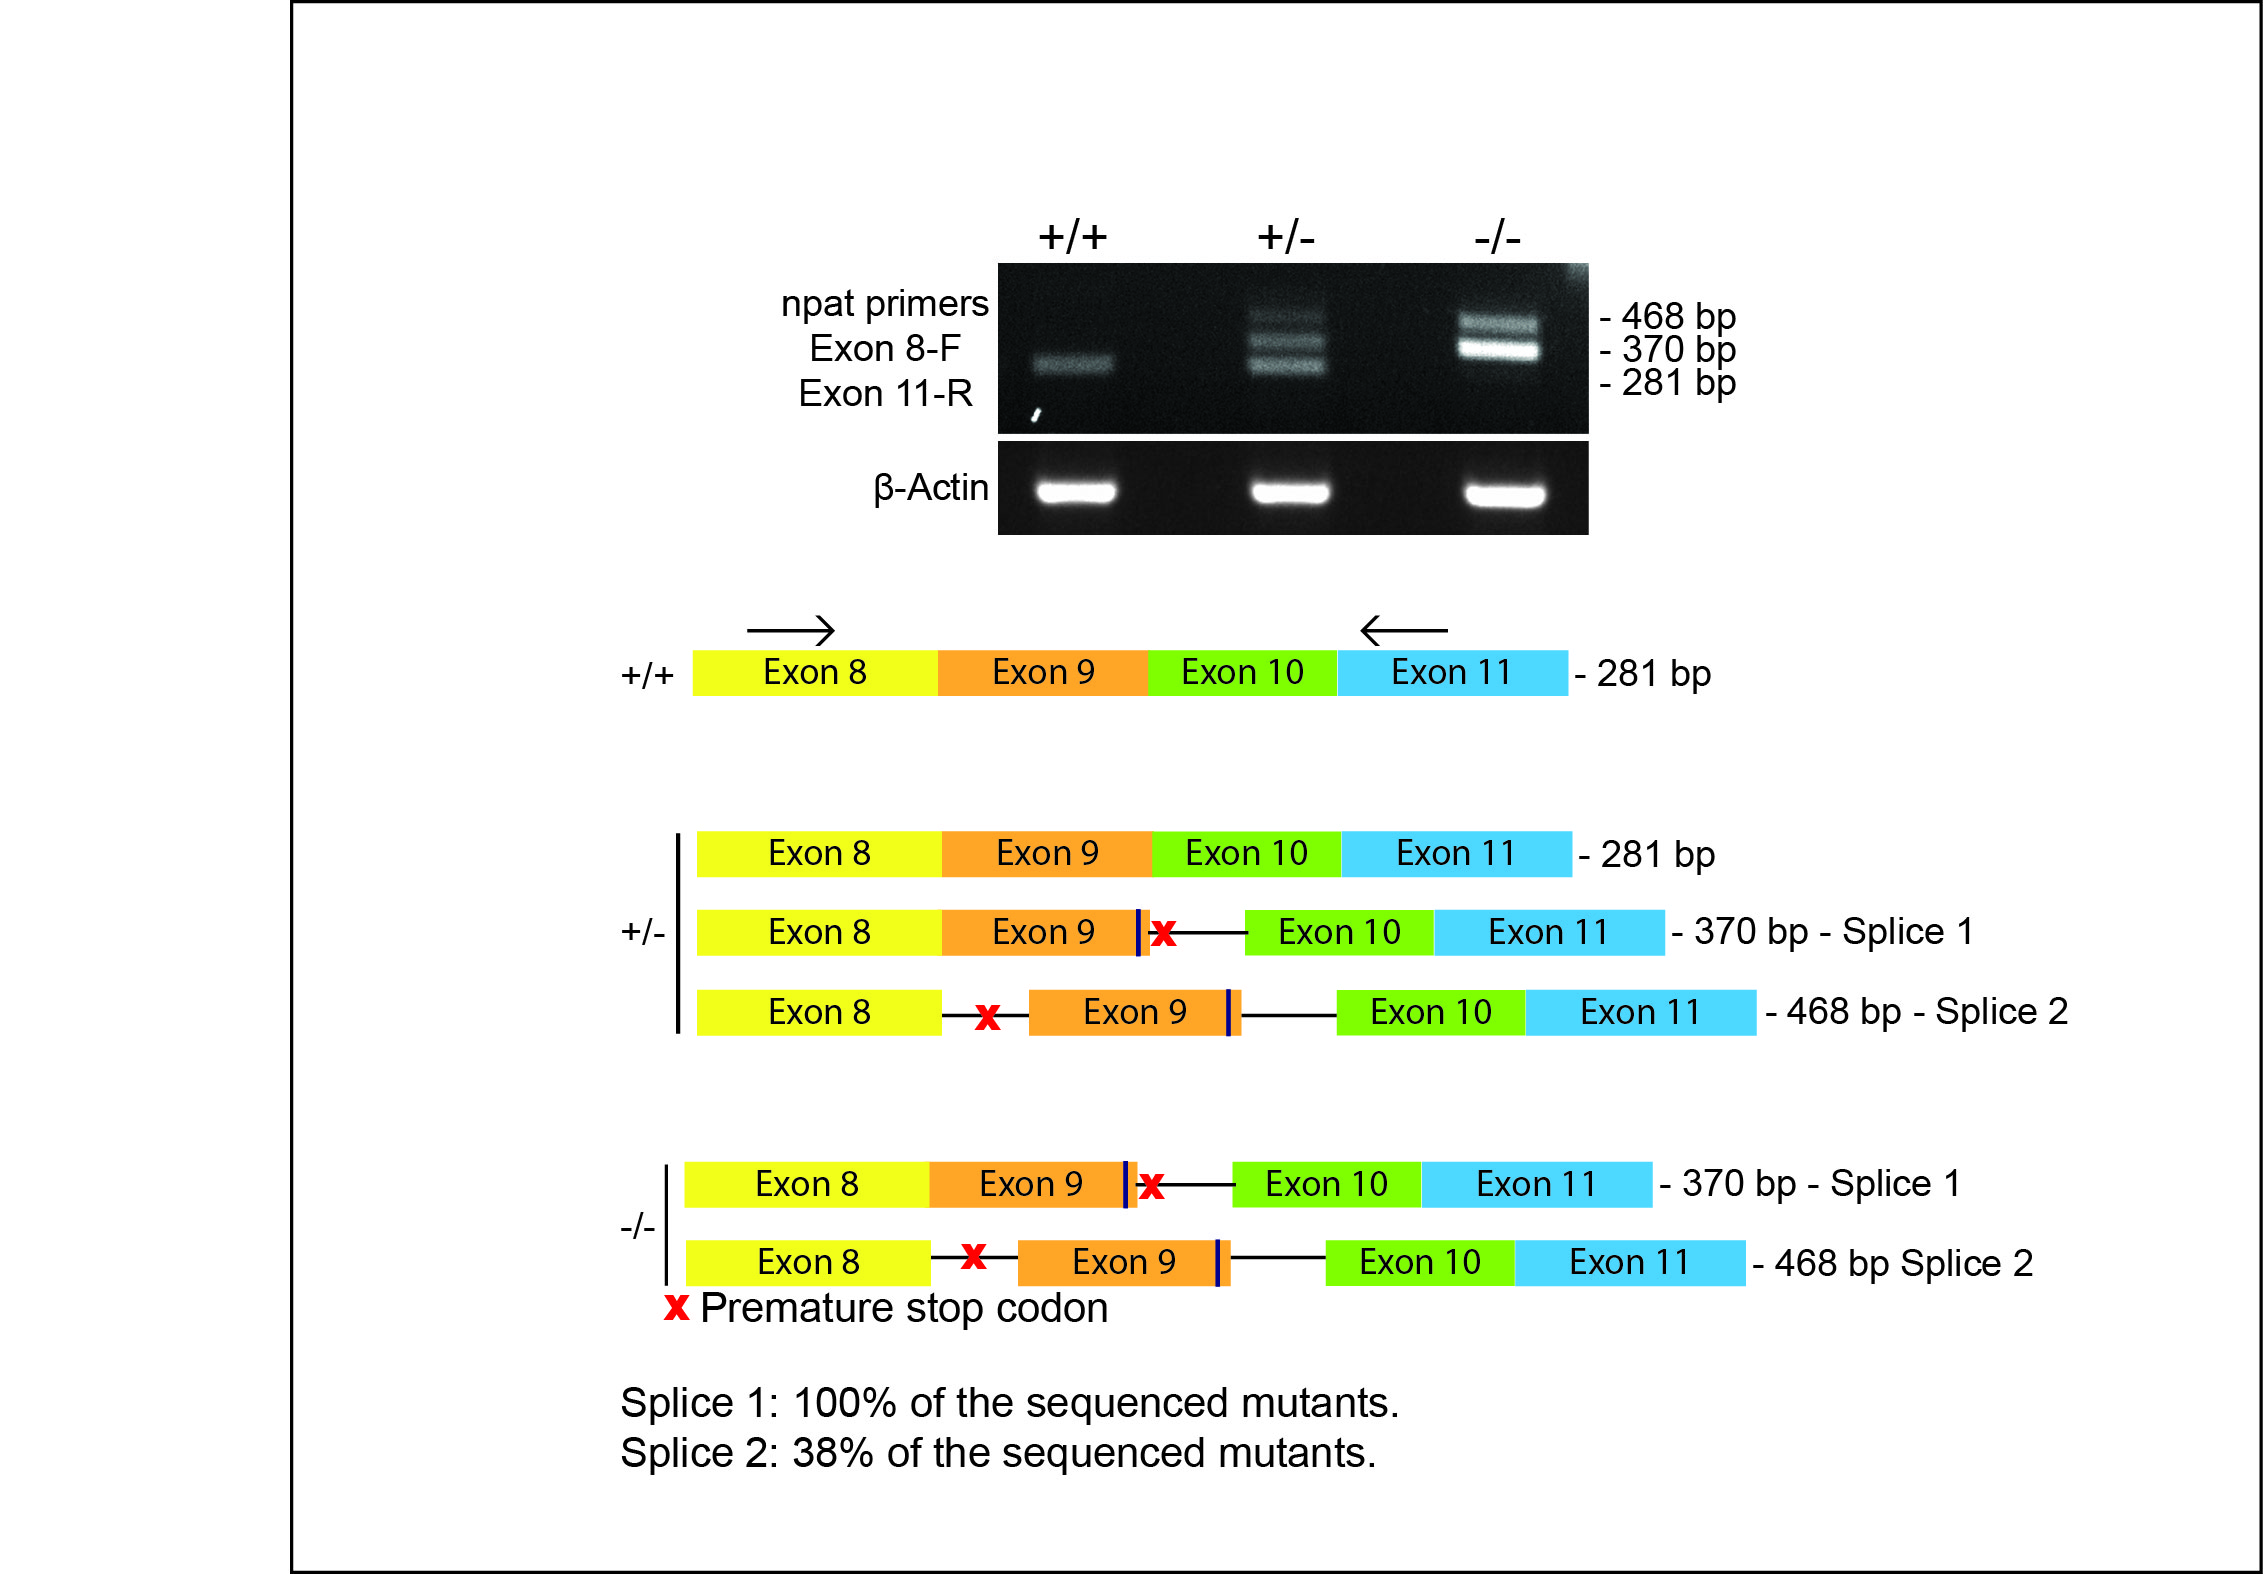
\includegraphics[width=.8\textwidth]{rys/PCRE8-E11WtSibRys.jpg}}    
    \caption{{\bf RT-PCR analysis reveals two aberrant intron retention variants in \textit{rys} mutant npat transcripts}}
    \label{npattranscript}
    Top panel: Agarose gel electrophoresis of mRNAs prepared from 3dpf homozygous wild type (+/+), heterozygote (+/-), and homozygous mutant (-/-) animals, as identified by genomic PCR. Fragments were amplified from a forward primer sited in exon 8 and a reverse primer sited in exon 11.
    Bottom panel: exon/intron layout schematics of the putative transcripts detected.
\end{figure}

\begin{figure}[!h]
    \makebox[\textwidth][c]{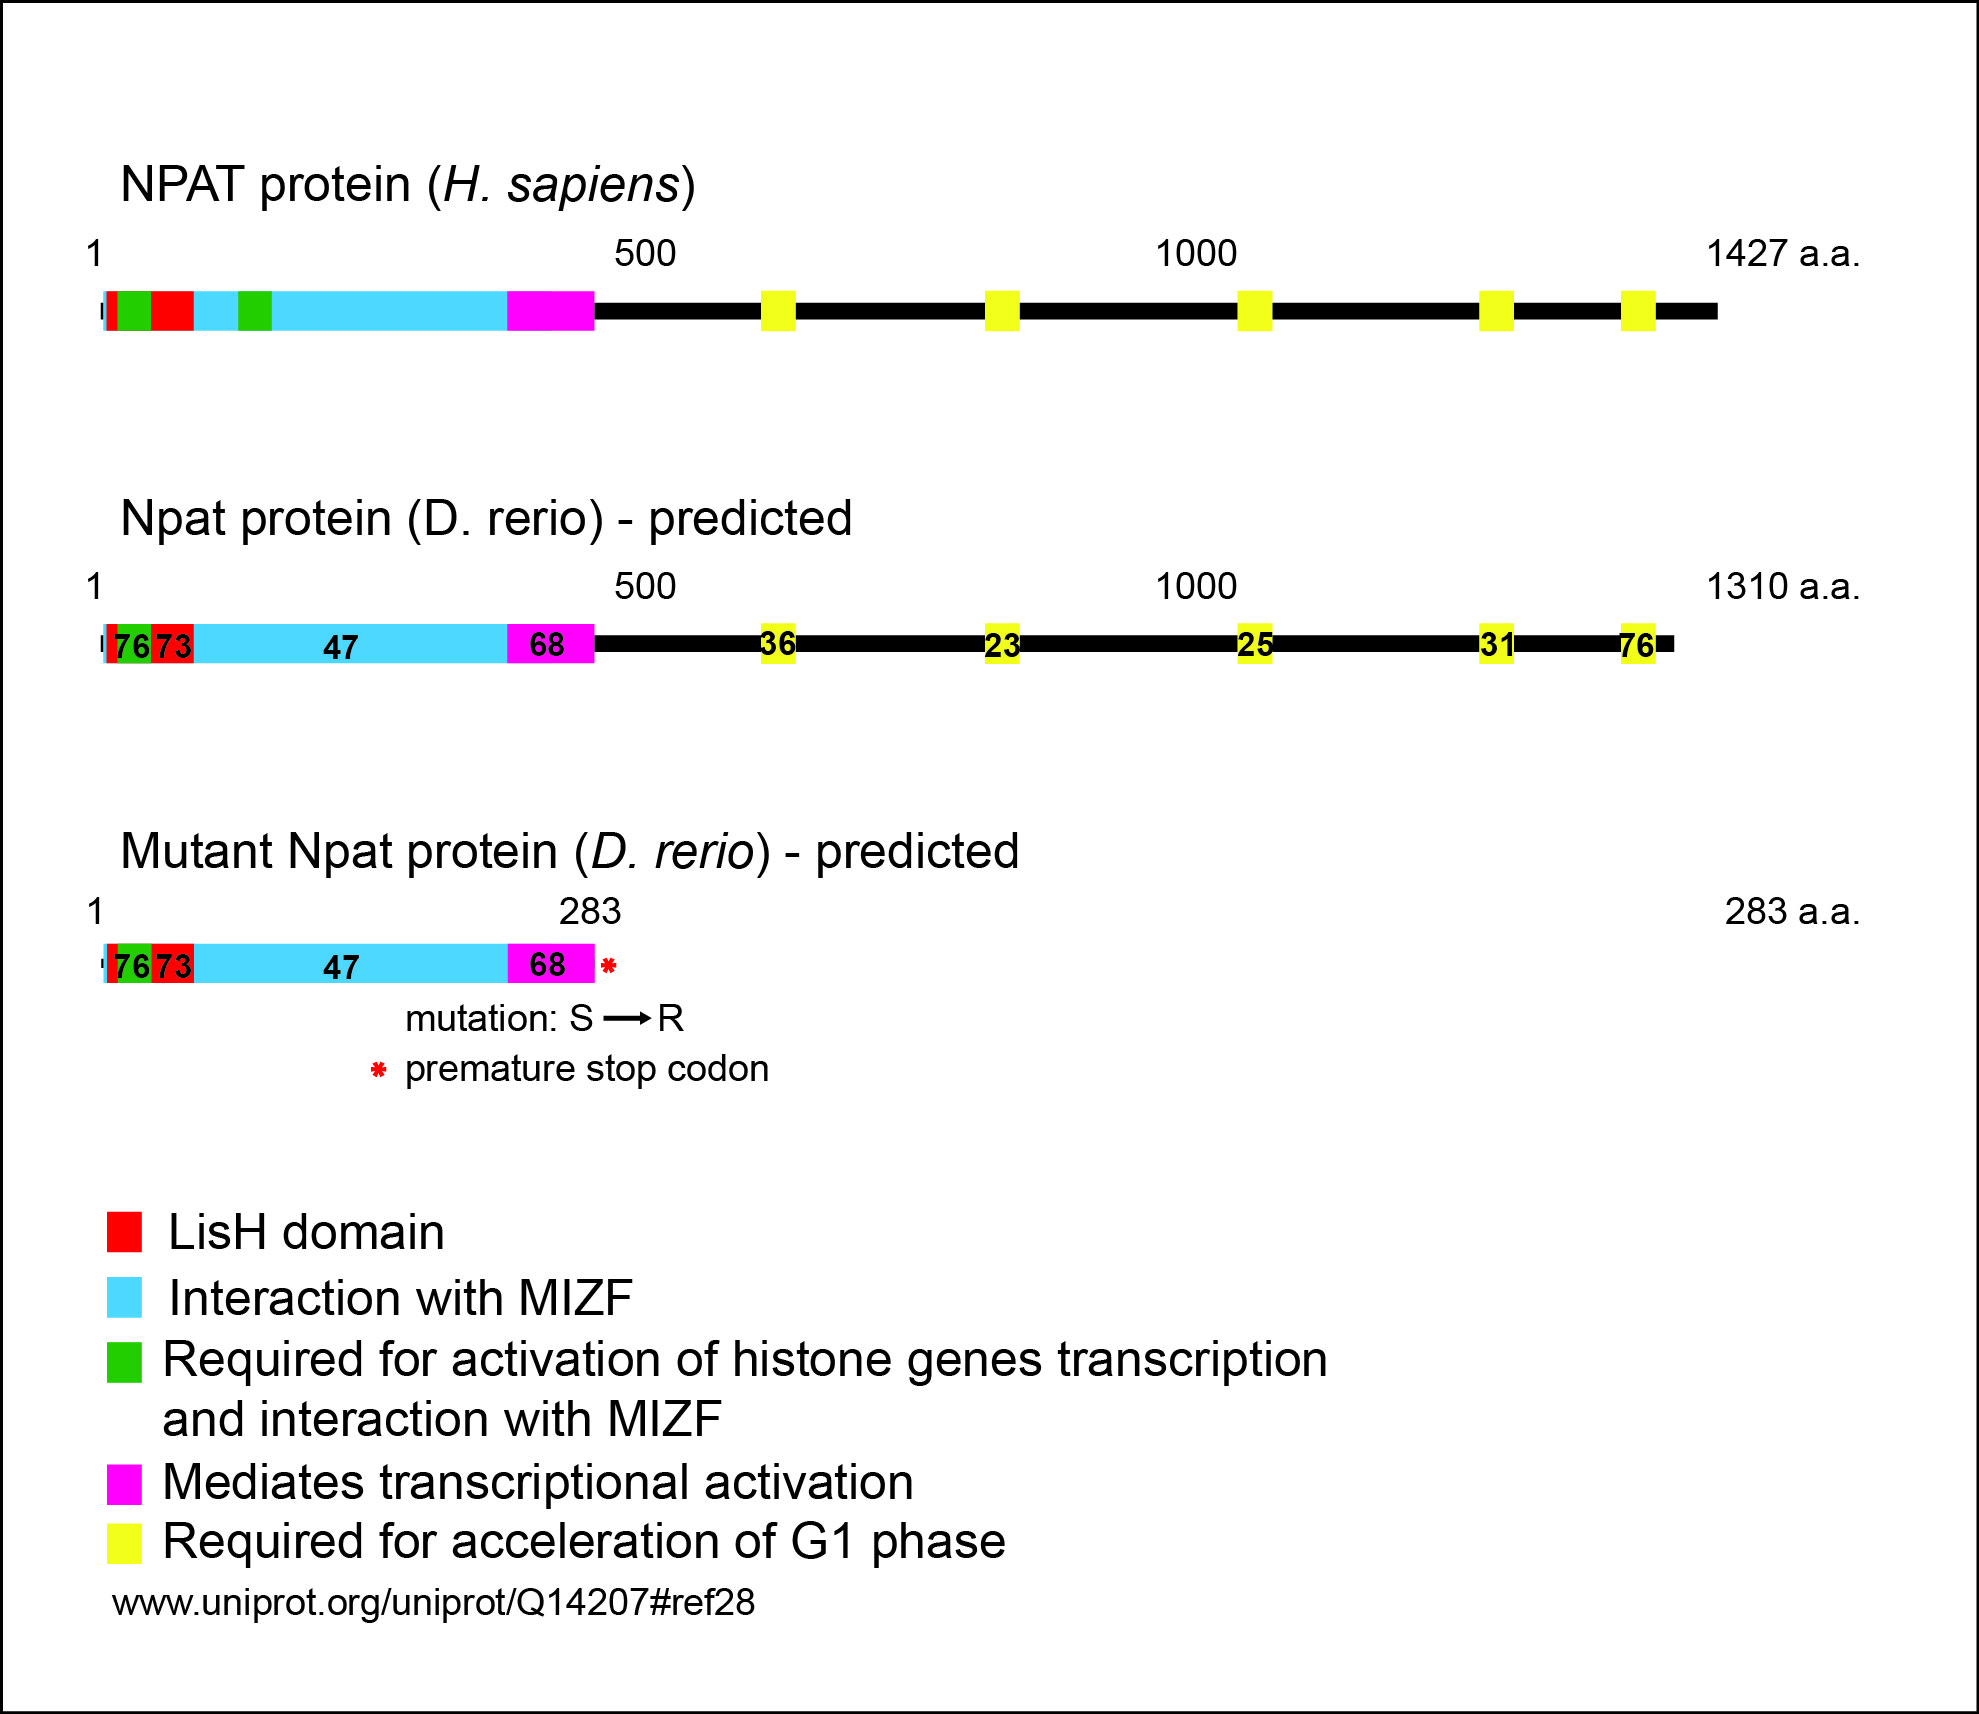
\includegraphics[width=.8\textwidth]{rys/Npat protein.jpg}}    
    \caption{{\bf Functional domains of Human NPAT compared to predicted wild-type and \textit{rys Danio} npat}}
    \label{npatprotein}
\end{figure}
\FloatBarrier

Because \textit{D. rerio} is a teleost known to have undergone genome duplication in an ancestral clade, we used the Synteny Database tool \cite{Catchen2009} identify any possible duplicates; plausibly, a duplication in zebrafish npat could explain the lessened severity of the mutant phenotype when compared to mammalian proviral inactivants. The results of this analysis are presented in Supplementary \autoref{synteny}. While npat is in the midst of a region which appears to be duplicated on chromosomes 5 and 15, relative to the unduplicated homologous syntenic run on \textit{H. sapiens} chromosome 11, it is not, itself, duplicated.

We performed in situ hybridisation using a probe directed to the wild type npat transcript to confirm that the gene is indeed expressed in wild type CMZs; we found that npat expression is progressively restricted to the CMZ from 4 to 6 dpf in wild-type fish. A representative time-course of 20 \si{\micro\metre} cryosections through ISH-treated embryos is depicted in \autoref{npatISH}, focusing on the retina at the times when it has formed. While npat remains transcribed in both the specified GCL and amacrine-rich inner INL to a degree, it is most intensely expressed in the proliferative CMZ, as we might expect on the basis of its cell cycle functions.

\begin{figure}[!h]
    \makebox[\textwidth][c]{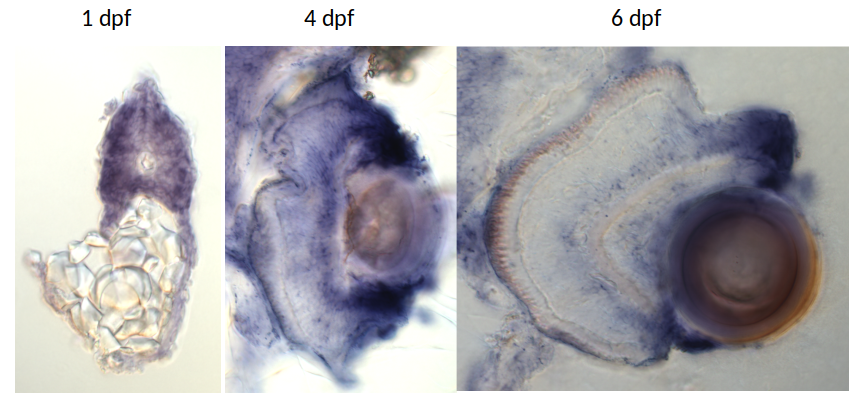
\includegraphics[width=.8\textwidth]{rys/ISH.png}}    
    \caption{{\bf In situ hybridization reveals progressive restriction of npat expression to the CMZ}}
    20\si{\micro\metre} sections of wild-type embryo (1dpf) and retinae (4 and 6 dpf), displaying progressive restriction of npat expression as assayed by in-situ hybridisation.
    \label{npatISH}
\end{figure}

Having taken note of the unusual chromatin ultrastructure present in \textit{rys} CMZ RPCs, and with a mutant npat allele reliably linked to the appearance of the \textit{rys} phenotype, we investigated the transcriptional status of npat and its histone regulatory targets in these animals. We first assayed npat itself by RT-PCR, finding that homozygous \textit{rys} mutants overtranscribe npat by about 3-fold compared to their wild-type counterparts at both 6dpf and 8dpf, while sibling overabundance declines from about 2.5-fold to 1.5-fold over this time period, as shown in \autoref{npatrtpcr}, with calculated marginal posterior mean mass over the WT standard given in \autoref{rtpcrtable}.

Since mammalian NPAT is known to regulate histone transcription and is critical for coordinating the correct expression of replication-dependent histone transcripts required to package genomic DNA during S-phase \cite{Zhao2000}, we hypothesized that the altered nuclear morphology and truncated S-phase we observed in proliferating \textit{rys} CMZ cells may be a consequence of perturbed regulation of histone transcription. To test this, we performed qPCR on random-hexamer-primed cDNAs produced from 6 and 8dpf wild type, sibling, and \textit{rys} embryo mRNA extracts. These qPCR assays were performed using degenerate primers\footnote{Zebrafish have notably populous histone clusters with numerous variants and pseudogenes not present in non-genomically-duplicated vertebrates, so degenerate primers are an appropriate way to survey the population of transcripts. A full catalogue has not been undertaken, to my knowledge.} directed toward all members of the zebrafish core histone gene families H2A, H2B, H3 and H4. As a role for NPAT in 3’ end processing of histone transcripts has been identified \cite{Pirngruber2010}, we also set out to determine whether 3’ end processing of histone transcripts is altered in \textit{rys}. By repeating the above-described qPCR assays on oligo-dT-primed cDNAs, we were able to examine the population of polyadenylated histone transcripts in isolation. 

\begin{figure}[!h]
    \makebox[\textwidth][c]{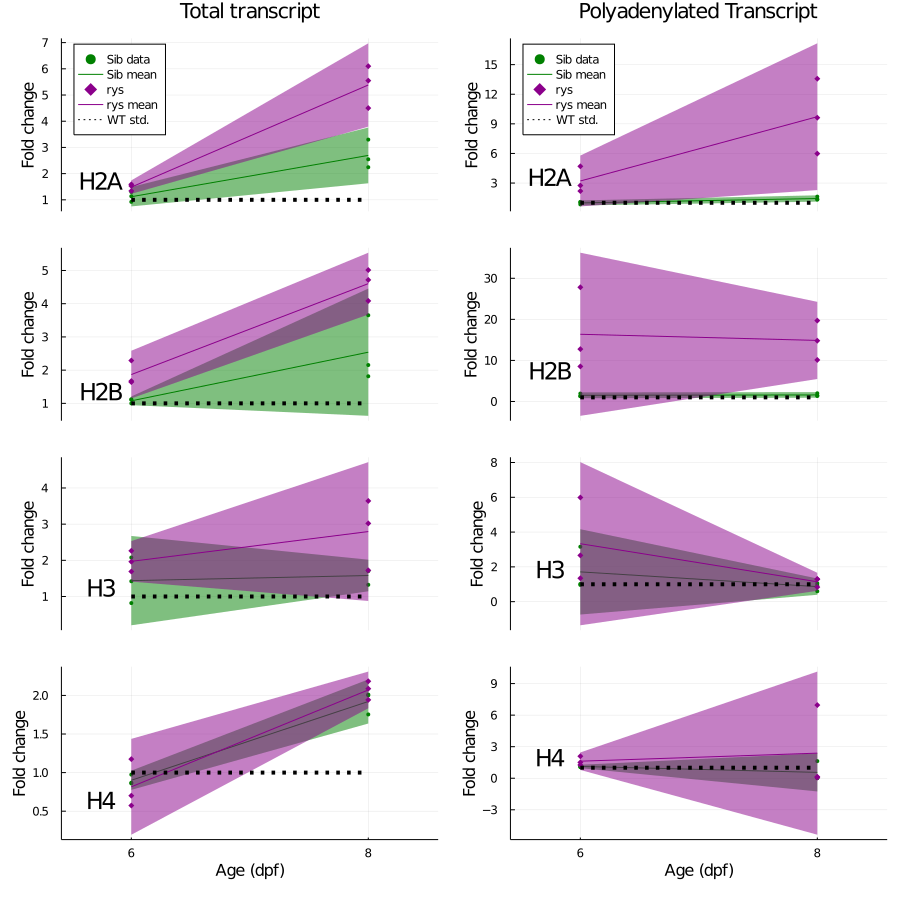
\includegraphics[width=.8\textwidth]{rys/qPCR.png}}    
    \caption{{\bf \textit{rys} overexpress total and polyadenylated core histone transcripts}}
    qPCR results for degenerately-primed families of core histone transcripts, from random hexamer primers for panels A and B, measuring total core histone transcripts, and oligo-dT for panels C and D, measuring polyadenylated transcripts. Panels A and C display results from cDNAs of 6dpf \textit{rys} mutants and siblings compared to wild-type conspecifics, while B and D are from 8dpf animals.    
    \label{histonertpcr}
\end{figure}

To plausibly be implicated in the \textit{rys} phenotype, a candidate histone transcript ought to be overexpressed in mutants relative to both WT and siblings at 6dpf and 8dpf. In order to determine the best-supported candidates for causative involvement in \textit{rys}, we calculated the standard deviations of significance which obtain on the test of mean rys transcript being greater than either mean sibling transcript or the WT standard (set to 1.0). These values are presented in \autoref{qPCRstds}.

\begin{table}[!ht]
    \centering
    \caption{{\bf Standard deviations of significance for \textit{rys} mutant transcript $>$ sib or WT}}
    \begin{tabular}{|l|l|l|l|l|} 
        \hline {\bf Pool} & {\bf Transcript} & {\bf Age} & {\bf Sib mean $\sigma$} & {\bf WT std $\sigma$}\\ \hline 
        Total & H2A & 6 & 1.59 & 3.72\\ \hline
        Total & H2A & 8 & 2.75 & 5.4\\ \hline
        Total & H2B & 6 & 2.12 & 2.37\\ \hline
        Total & H2B & 8 & 1.9 & 7.59\\ \hline
        Total & H3 & 6 & 0.77 & 3.39\\ \hline
        Total & H3 & 8 & 1.21 & 1.83\\ \hline
        Total & H4 & 6 & -0.26 & -0.58\\ \hline
        Total & H4 & 8 & 0.79 & 8.83\\ \hline
        polyA & H2A & 6 & 1.68 & 1.68\\ \hline
        polyA & H2A & 8 & 2.18 & 2.3\\ \hline
        polyA & H2B & 6 & 1.47 & 1.52\\ \hline
        polyA & H2B & 8 & 2.76 & 2.89\\ \hline
        polyA & H3 & 6 & 0.6 & 0.97\\ \hline
        polyA & H3 & 8 & 0.78 & 0.54\\ \hline
        polyA & H4 & 6 & 1.15 & 1.46\\ \hline
        polyA & H4 & 8 & 0.45 & 0.35\\ \hline
    \end{tabular}
    \label{qPCRstds}
\end{table}

Following these calculations, we find the greatest significance at 6dpf for the \textit{rys} overexpression of total H2B transcript, followed by polyadenylated H2A, total H2A, and polyadenylated H2B. The ordering for 8dpf is similar: the most significant overexpression results are for polyadenylated H2B, then total H2A, polyadenylated H2A, and total H2B. We note that the overabundances of polyadenylated H2A and H2B are approximately 2-20 fold greater than those observed for any other transcript pool or histone family. 

We assess the joint probability that mean \textit{rys} mutant total H2A is greater than the sib mean at both 6dpf and 8dpf to be 99.7\% $\pm$ 5.0; the same figure for H2B is 98.5\% $\pm$ 5.1. The joint probability that mean total H2A and H2B are elevated in \textit{rys} mutants compared to sibs at both ages is therefore 98.2\% $\pm$ 7.1. For the polyadenylated transcripts, the joint probability that the \textit{rys} mutant polyA H2A mean is greater than the sib mean at both ages is 94.1\% $\pm$ 9.9; the same figure for H2B is 92.6\% $\pm$ 3.3. The joint probability that mean polyadenylated H2A and H2B are elevated in \textit{rys} relative to sibs at both ages is then 87.1\% $\pm$ 9.7. On the basis of these calculations, we suggest the most plausible causal contributor to the \textit{rys} phenotype, of the transcript families examined, are H2A and H2B transcripts. While the relative magnitude of the overabundance of total H2A and H2B transcript is less than that of the polyadenylated pool, we have significantly less uncertainty about these figures. Still, the polyadenylated transcript results seem to speak to a fundamnetal loss of control over the abundance of these gene products; unlike the total transcript pool, siblings retain tight, WT-like control over polyadenylated transcripts, while \textit{rys} mutants display much more extensive variability in polyA transcript expression, even where the mean is not elevated above siblings or WT controls.

\begin{figure}[!h]
    \makebox[\textwidth][c]{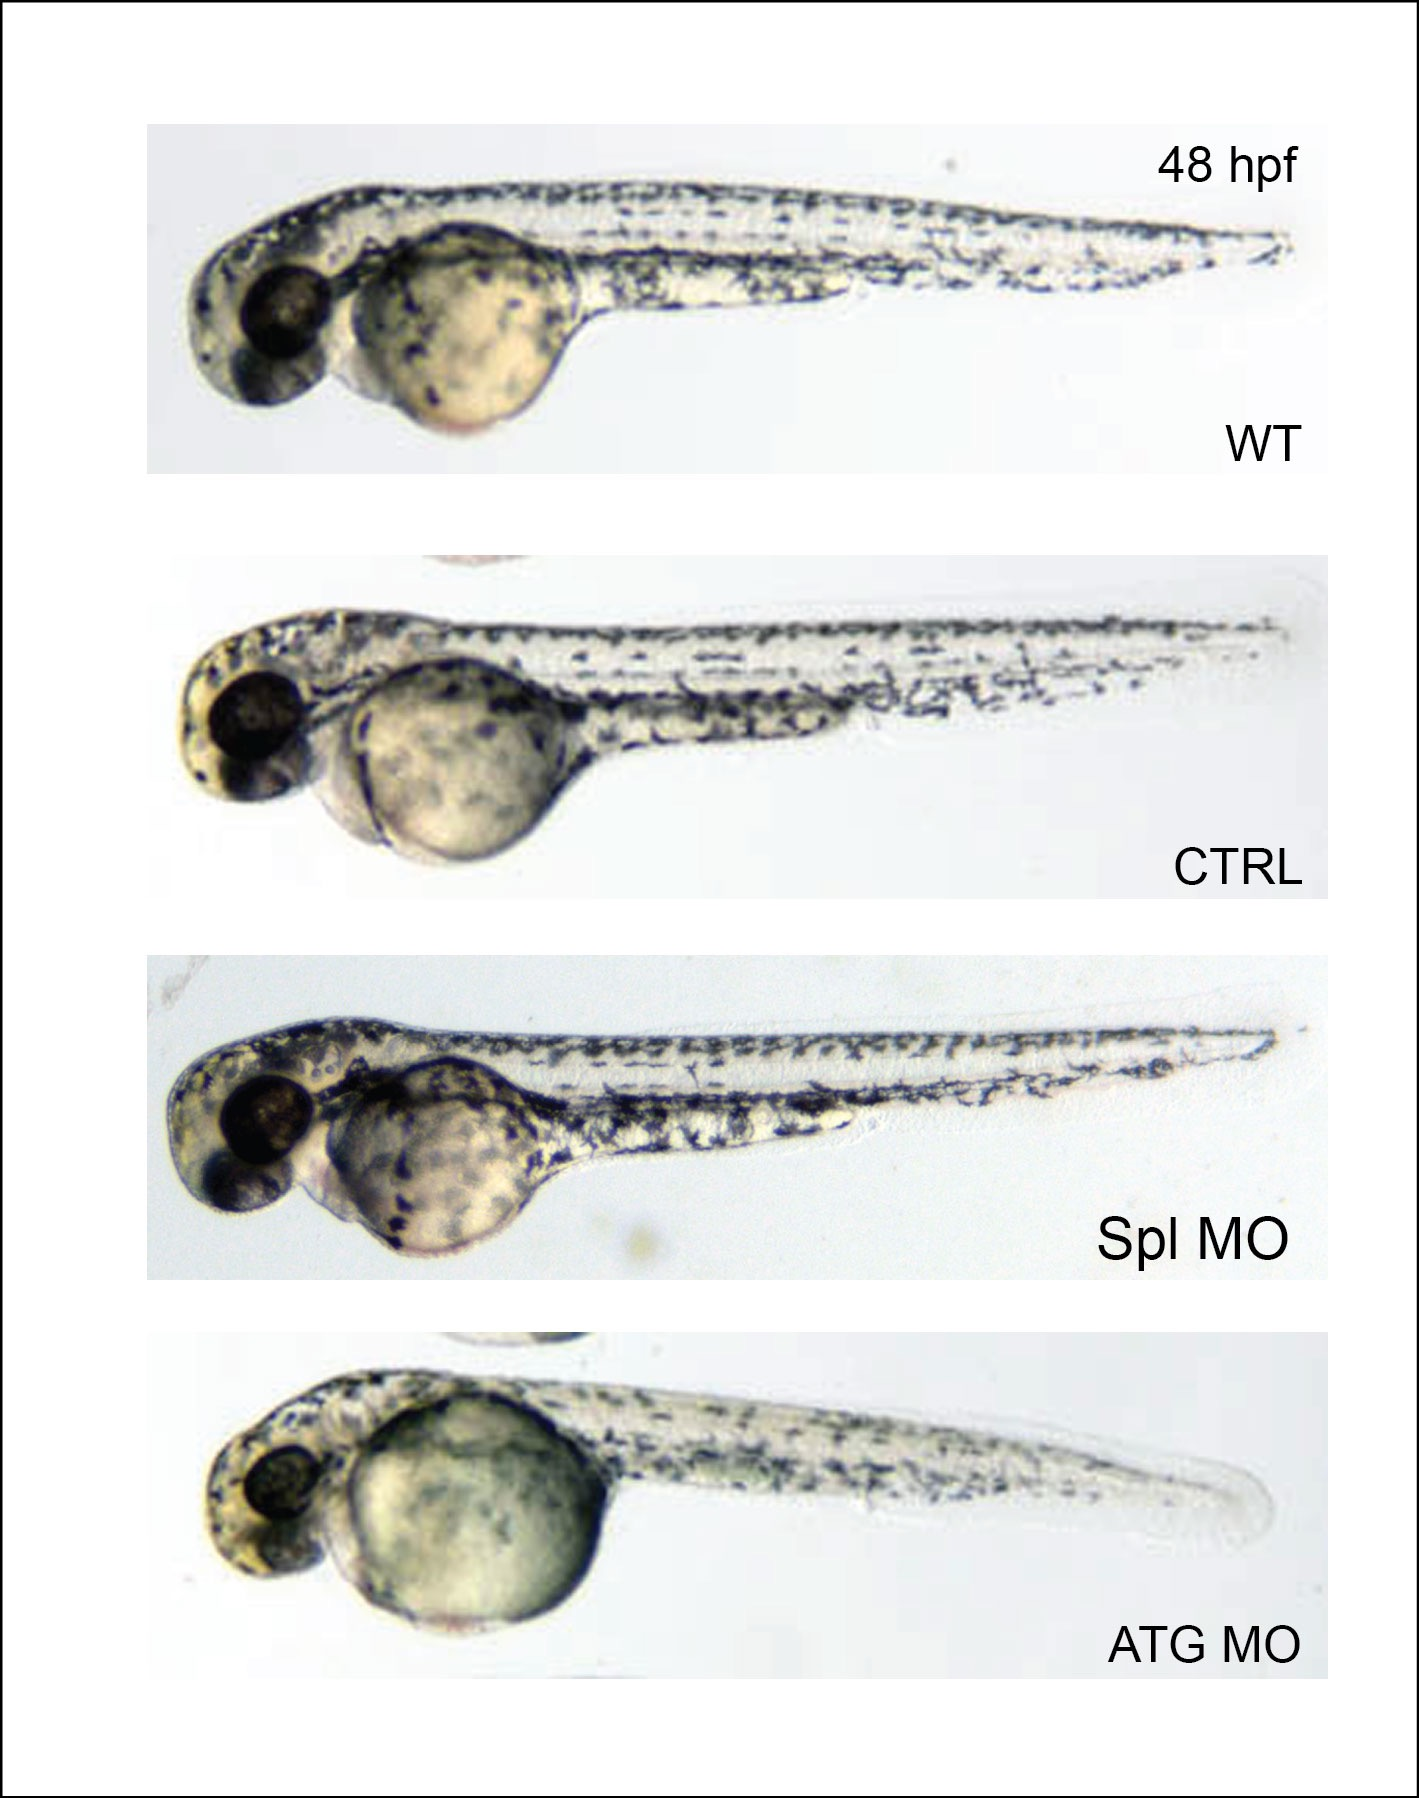
\includegraphics[width=.7\textwidth]{rys/morpholinos.jpg}}    
    \caption{{\bf 48hpf embryos injected with an npat ATG-targeted morpholino display a small-eye phenotype}}
    20\si{\micro\metre} sections of wild-type embryo (1dpf) and retinae (4 and 6 dpf), displaying progressive restriction of npat expression as assayed by in-situ hybridisation.
    \label{morpholinopics}
\end{figure}

While these observations substantiate the involvement of npat in the \textit{rys} phenotype, we pursued the matter further by perturbing npat using morpholino injections of wild-type fish. As we do not suppose morpholino transcriptional blockade will precisely replicate the cellular conditions of a genetic null some days after birth, we did not seek to recapitulate the \textit{rys} phenotype. Rather, we sought to determine if any of \textit{rys}'s constituent phenomena would appear after an early blockage of \textit{rys} transcription, further substantiating the general involvement of npat in \textit{rys}. We tested morpholinos directed both to the npat start codon and to the splice site affected in \textit{rys}, alongside control morpholinos and uninjected animals. We used both a morpholino directed to the transcript ATG start site, as well as to the affected splice site. 

The splice morpholino consistently replicated the \textit{rys} phenotype on both total and polyadenylated core histone transcript abundance, while the ATG morpholino more narrowly replicated the effect on polyadenylated transcript (\autoref{morpholinoRTPCR}). The ATG morpholino produced animals with small eyes by 72dpf, as shown in \autoref{morpholinopics}. We also conducted an analysis of the nuclear morphological parameters measured in \autoref{nuclearstudy} for \textit{rys} mutants and siblings. For each of the ATG and splice morpholinos, we estimated the joint evidence for separate experimental morpholino and control morpholino models against a combined model. The evidence calculations are presented in Supplementary \autoref{morpholinoev}. We found substantial evidence in favour of separate models for the ATG and control morpholino effects on the number of central retinal neurons per CMZ cell, confirming our observation of overall decreased eye size in ATG morpholino-injected animals. These results establish that the identification of npat as the causative mutation in \textit{rys} is plausible, as experimental perturbation to npat in WT fish can result in \textit{rys} phenotypic phenomena, notably overexpression of core histone transcripts and small eyes arising from a decrease in the population of the central retina without a concomittant decrease in CMZ population. 

\begin{figure}[!h]
    \makebox[\textwidth][c]{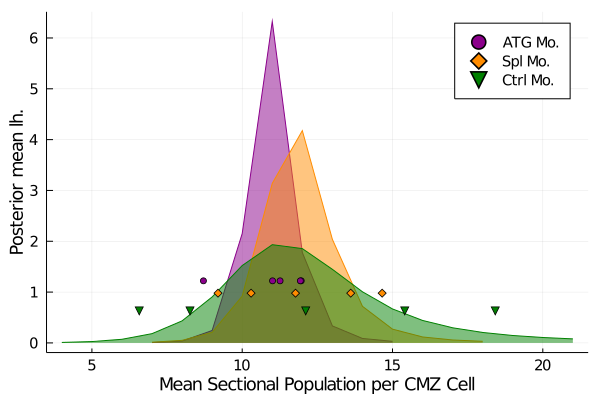
\includegraphics[width=.75\textwidth]{rys/morphnuclei.png}}    
    \caption{{\bf ATG morpholino perturbation of npat recapitulates decline in mean  central retinal population relative to CMZ}}
    \label{morphonucstudy}
\end{figure}

\subsection{\textit{rys} siblings and mutants have unique sets of nucleosome positions, best explained by different sequence preferences and increased sequence-dependent positioning in mutants}
 Our observation of perturbed histone expression in \textit{rys} embryos led us to suspect that the aberrant nuclear morphology observed in \textit{rys} CMZ progenitors arises from disrupted chromatin organisation, which is a possible consequence of altering the dynamic composition of the histone pool available for nucleosome formation during cell cycle. We therefore sought to characterise nucleosome positioning in \textit{rys} and wild-type siblings by micrococcal nuclease (MNase) digestion of pooled genomic DNA (gDNA). Nucleosome-protected fragments from the MNase digests were sequenced and positions called as described previously.


 \begin{figure}[!h]
    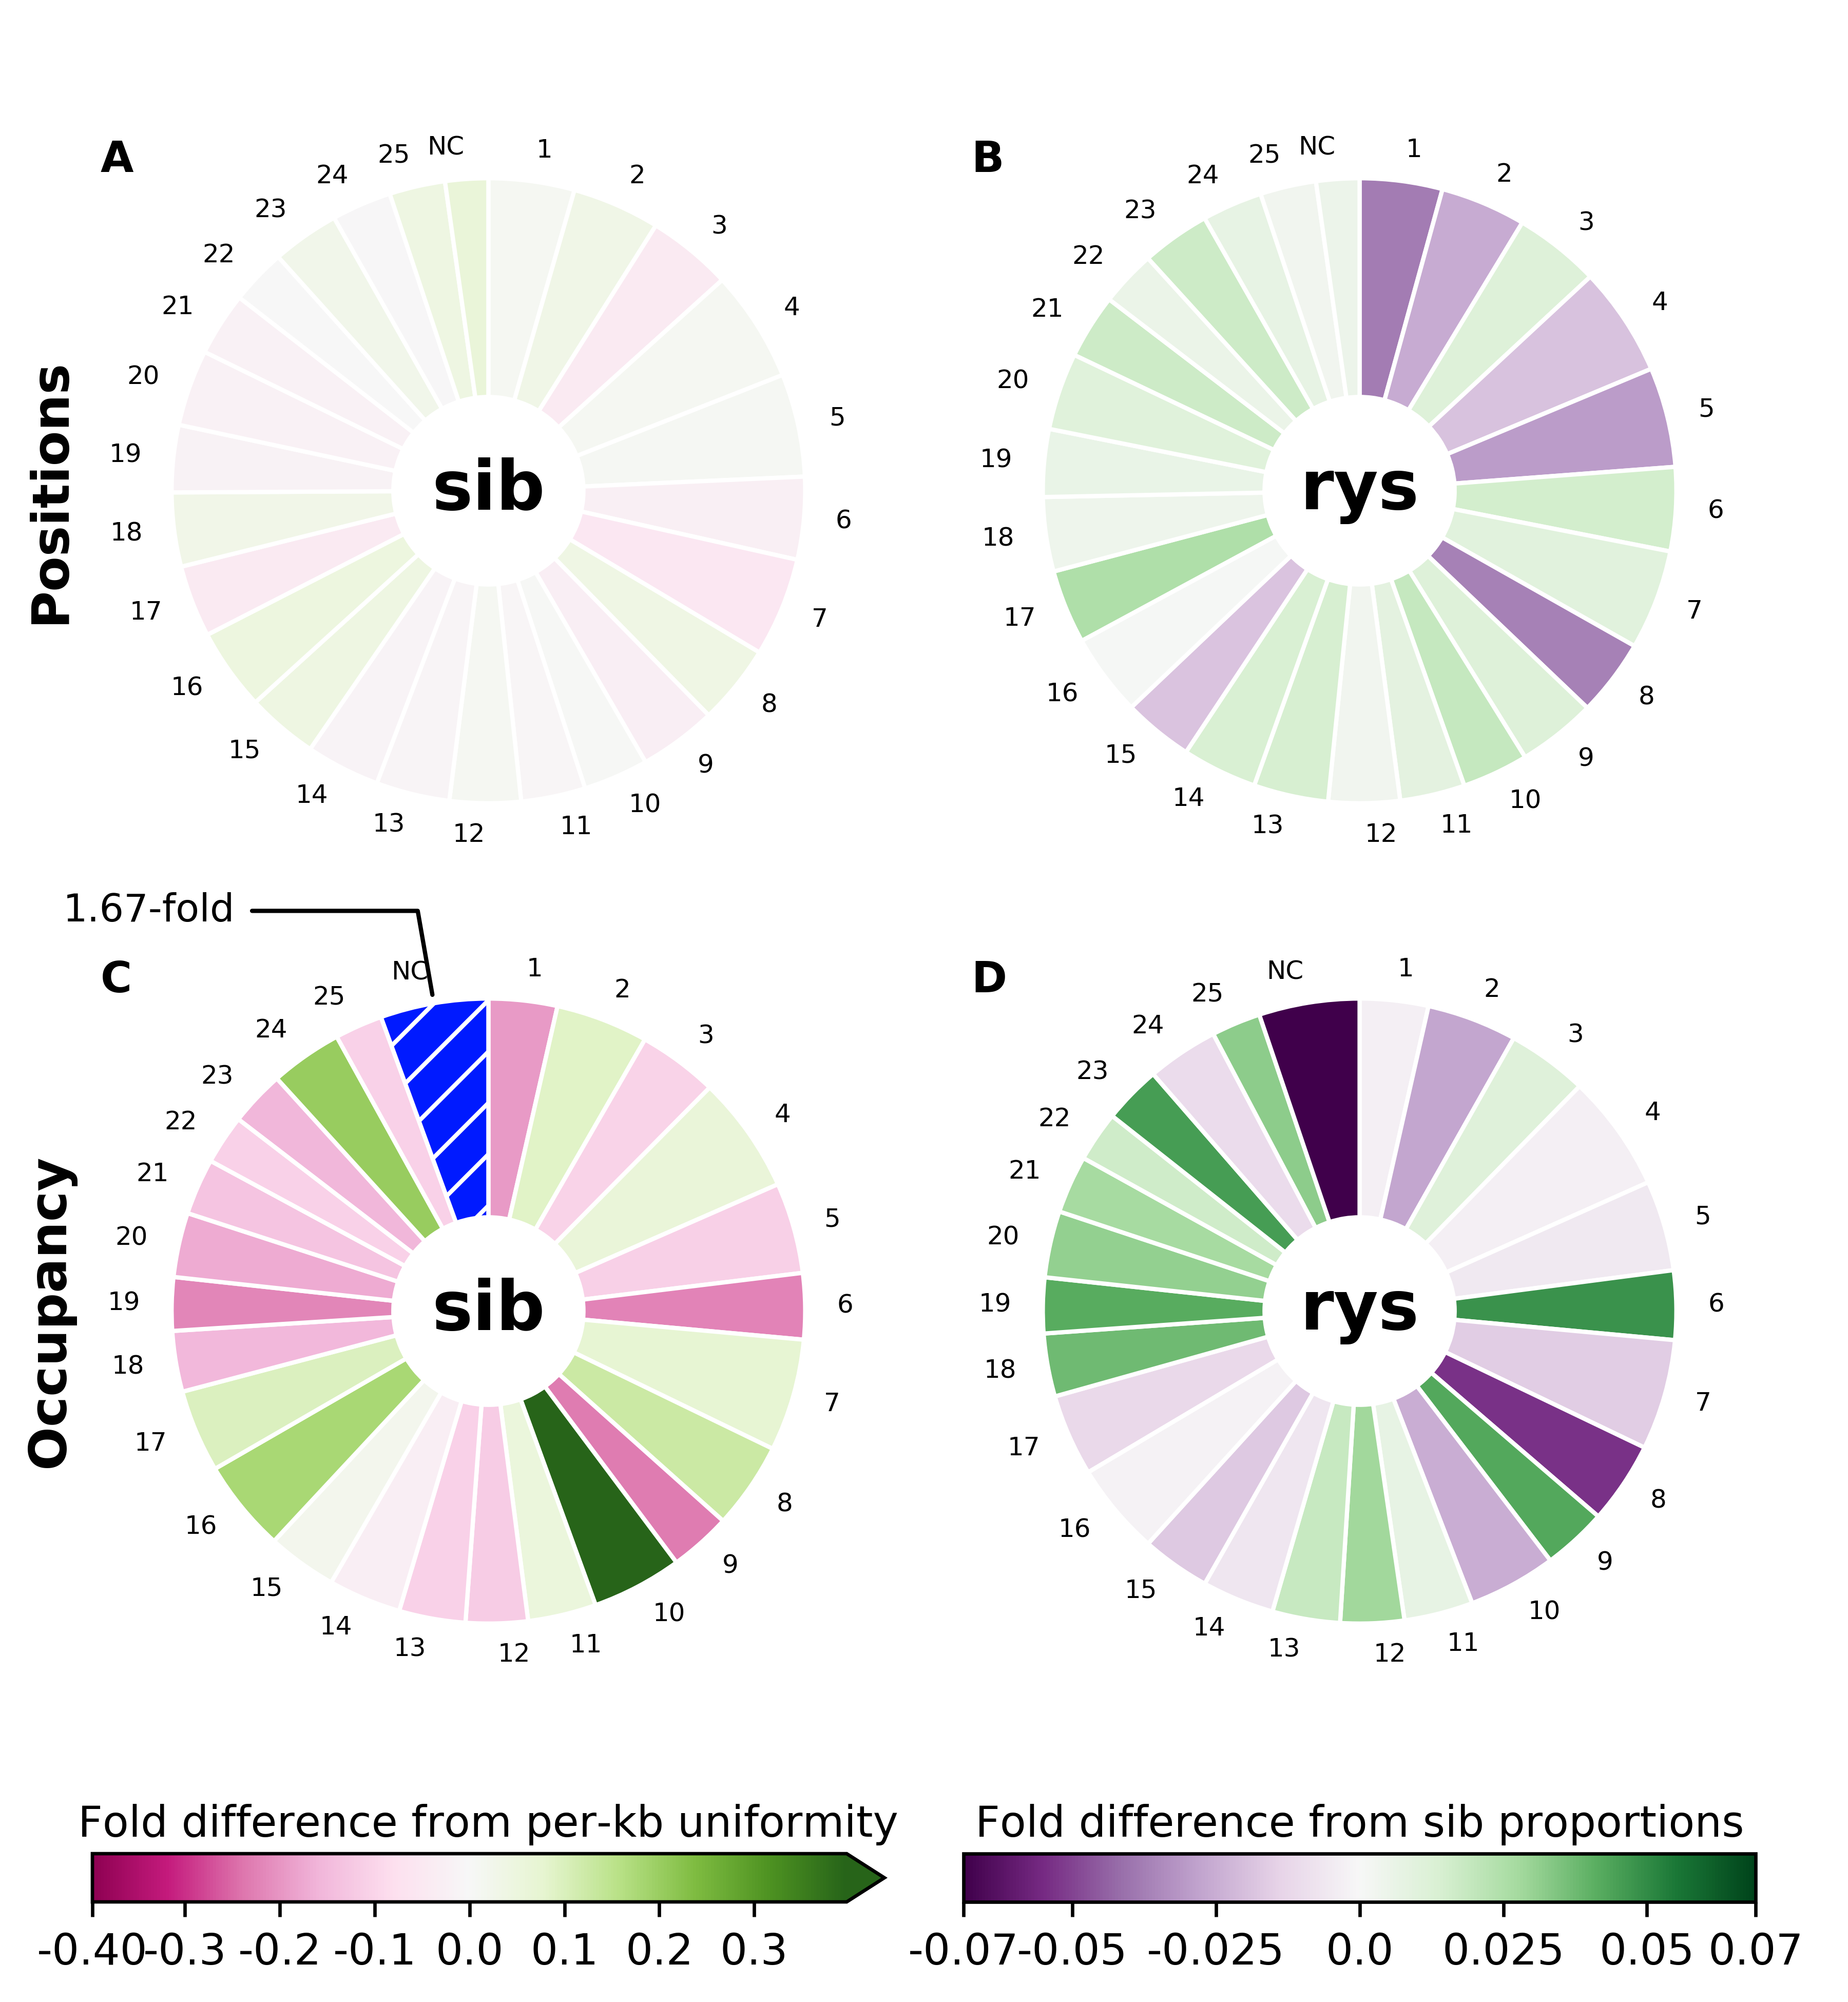
\includegraphics{rys/proportional_chromosome_occupancy.png}
    \caption{{\bf \textit{rys} chromosomes are differentially enriched and depleted of nucleosome position density and occupancy.}}
    Pie charts of nucleosome position density and occupancy by chromosome. Width of pie slices in panels A and B indicates the fraction of the total number of positions occuring in the numbered chromosomes and nonchromosomal scaffolds (NC). In panel A, depicting the sib genome, slices are colored according to the extent of deviation from an assumption of even distribution of nucleosomes across the genome. In panel B, depicting the \textit{rys} genome, slices are colored according to the extent of deviation from the sib distribution. The width of slices in slices B and D indicate the fraction of the total nucleosome occupancy signal detected. Slice coloration depicts deviations from nucleosome occupancy distributions analogous to position distributions in A and B. Blue and white diagonal bars in the NC slice of panel C denote an out-of-scale positive deviation from the assumption of even distribution, i.e., sib NC scaffolds have 1.67-fold more of the total nucleosome occupancy signal than is expected from their length alone.  
    \label{nucgendist}
    \end{figure}
    
 We first examined the genomic disposition of nucleosome positions within wild-type siblings and \textit{rys}. We found nucleosome positions distributed relatively evenly over sib genomic material, with only tiny deviations from a neutral assumption of a uniform distribution of the total position number over the full length of the genome, as displayed in Fig. \ref{nucgendist}, panel A. Bulk \textit{rys} chromatin displays minor differences from the proportions of positions found in each sib scaffold (panel B). Sib nucleosome positions are differentially occupied across scaffolds, with Chr 10 and scaffolds not yet mapped to chromosomes (NC) being notably more occupied than expected from scaffold length alone (panel C). Similarly to the distribution of positions, \textit{rys} chromatin is somewhat more evenly occupied than sibs; scaffolds with positions that are more heavily occupied in sibs tend to be depleted in \textit{rys} and vice versa (panel D). 


\begin{figure}[!h]
    \makebox[\textwidth][c]{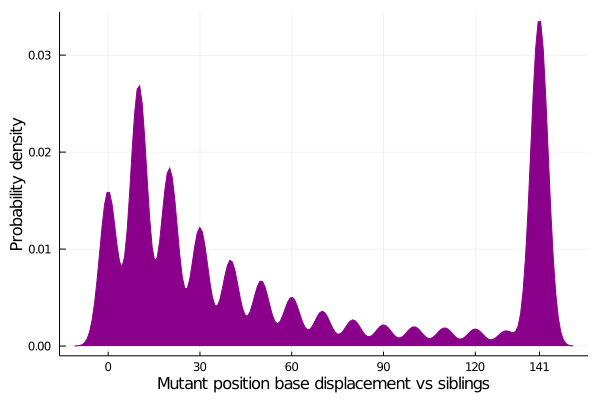
\includegraphics[width=.75\textwidth]{rys/shiftdist.png}}    
    \caption{{\bf PWM sources detected in sibling differential nucleosome positions.}}
    Probability distribution of \textit{rys} position displacement distance from mapped sibling positions, in base pairs. 
    \label{shiftdist}
\end{figure}

By mapping the called nucleosome positions in rys to those in sibs, and calculating the number of bases the \textit{rys} position is displaced from its mapped position, we characterised the population of \textit{rys} positions by translational displacement from the arrangement found in siblings. The probability distribution of this displacement parameter for the population of \textit{rys} positions is displayed in \autoref{shiftdist}. The notable bimodality of this distribution arises as a result of the inclusion of unmapped positions, to show the relative size of this population: 23\% of positions are not mapped to any sibling position at all; these are located at 141, the full length of a called nucleosome position in our pipeline. The other three-quarters of the positions are mapped to sibling positions, with 11\% of overall \textit{rys} positions coinciding entirely with the sibling positions, 19\% displaced 10 bases or less from a sib position, and a further 21\% displaced between 10 and 30 bases. The last quarter of \textit{rys} positions display more extreme displacements, up to the entire length of the position. The periodic multimodality observed in the displacement distance of \textit{rys} positions relative to sibs is commonly observed in patterns of nucleosome positioning and arises from the 10-base perioicity of nucleosome contacts with DNA \cite{Wright2017}. This distribution of population displacement strongly suggests that the npat mutation in \textit{rys} results both in a loss of translational control of nucleosomes that are in approximately the expected positions, most commonly by a nucleosome ``roll''of one contact, as well as a loss of trans-acting nucleosome positioning control which gets nucleosomes to the correct positions to begin with, represented by the novel \textit{rys} positions, with no mapped sibling ounterpart.

Mindful of the whole-organism source of the nucleosomal genomic sample used to generate the called positions, and of the heterogenous nature of the \textit{rys} phenotype, with RPCs displaying the nuclear phenotype but not specified retinal neurons, the second, novel, group of positions mentioned above was of interest, as we sought to identify position subpopulations that might represent those involved in the nuclear phenotype. Interestingly, not only are there \textit{rys} nucleosome positions which are not found in siblings, but there is likewise a subset of sib positions which are never found to be occupied in rys . Intriguingly, sib positions which are not observed in rys are compensated for quite evenly across the genome by new positions gained in the mutants, with a small excess of new rys positions on most chromosomes, as shown in Supplementary \ref{diffposdist}.

This result suggested that a particular subpopulation of wild type nucleosomes are mislocalised in \textit{rys}. If the pool of available histones in proliferating \textit{rys} progenitors is substantially different from that of siblings, \textit{rys} nucleosomes forming from this pool may have altered physico-chemical interactions with DNA, which could result in a preponderence of nucleosomes with unusual sequence preferences. If so, this would explain the disappearance of a subset of positions in \textit{rys} and the appearance of a new, similarly sized subset of positions (the `differential set').

To formally address this hypothesis, we calculated the Bayesian evidence ratio for separate emission processes for sib and \textit{rys} position sequences against a combined process for both sets of sequences. If the molecular process resulting in the differential set arises from altered nucleosome composition in proliferating \textit{rys} cells, we expect these sequences to provide greater support for separate emission processes than for a single, combined process. On the other hand, if abberant DNA-nucleosome interaction is not causally relevant, and the reason for the apparently displaced nucleosomes is another macromolecular process, the evidence ratio should favour a combined process for the emission of the differential set- that is, there should be no difference between the unique sib and \textit{rys} sequences that would justify the additional complexity of separate models.

The emission model used was the Independent Component Analysis form described by Down and Hubbard \cite{Down2005}, with a fixed number of independent, variable length position weight matrices related to observations by a Boolean mixing matrix. An observation is scored by the background likelihood of its sequence, given some model of genomic noise, convolved with a sequence-length- and cardinality-penalized score\footnote{That is, the additional score provided by a source to an observation is penalized both by the expected number of motif occurrences given an observation of that length, as well as by the number of sources which explain the observation in the model.} for each source which the mix matrix indicates is present in the observation. Therefore, we first needed to construct background models of \textit{D. rerio}'s genomic "noise" from which repetitive sequence signals characteristic of nucleosome positions could be extracted. Following the suggestion of Down and Hubbard \cite{Down2005} that a principled approach to the selection of background models is to train and test a variety of them on relevant sequence, we used the Julia package BioBackgroundModels (presented in \autoref{ch:BBM}) to screen a panel of 1,2,4, and 6-state HMMS against  0th, 1st, and 2nd order encodings of samples from the zebrafish genome, partitioned grossly into exonic, periexonic, and intergenic sequences. We found that each of these partitions is best represented by 6-state HMMs trained on a 0th order genome encoding (i.e. the HMMs emit the 4 mononucleotides), as determined by model likelihood given an independent test sample, displayed in Supplementary \autoref{BHMMlh}.

We next used the Julia independent PWM component analysis nested sampling library BioMotifInference (presented in \autoref{ch:BMI}) to sample from the posterior distribution, given the differential set of \textit{rys} nucleosome positions and the composite background model of genomic noise. We initialized separate ensembles from uninformative priors on the \textit{rys} and sib data alone, as well as the combined \textit{rys} and sib data, allowing for 8 independent PWM sources in all cases. We compressed three model ensembles to within 125 orders of magnitude between the maximum likelihood model sampled and the minimum ensemble likelihood\footnote{That is, the convergence criterion was that the ensemble difference $log(L_{max})-log(L_{_min}$ be <125).}. This process produced the model evidence estimates summarized in \autoref{BMIevidencetable}, as well as maximum a posteriori samples for each of the ensembles. We estimate that there are greater than 360 orders of magnitude of evidence in favour of separate generative processes for the differential sib and \textit{rys} than for a combined model, with an estimated 525 standard deviations of significance. This large evidentiary weight and signficance give us statistical almost-certainty in selecting separate models for these sequences over a combined model.  We present the MAP PWM source samples from the better-evidentiated separate \textit{sib} and \textit{rys} models in \autoref{sibmotifs} and \autoref{rysmotifs} respectively, while the inferred combined sources are available in Supplementary \autoref{combinedmotifs}.

\begin{table}[!ht]
    \centering
    \caption{{\bf Evidence favours separate emission models for the \textit{rys} mutant and sibling differential position sets}}
    \begin{tabular}{|l|l|l|l|l|l|}
        \hline {\bf Sib logZ} & {\bf \textit{rys} logZ} & {\bf Joint Sib/\textit{rys} logZ} & {\bf Combined logZ} & {\bf logZR} \\ \hline
        -1.117572e6 ± 0.43 & -1.161415e6 ± 0.35 & {\bf -2.278988e6 ± 0.56} & -2.279356e6 ± 0.42 &  368.5 ± 0.7 \\ \hline
        \end{tabular}
    \label{BMIevidencetable}
\end{table}

BioMotifInference's source detection was highly conservative, likely due to the good quality of the background models, which were found to explain a majority of observed nucleosome positions adequately, without any PWM sources, in most models of the maximum a posteriori estimate, for both sibling and rys ensembles. In siblings, the top three sources are the only ones detected in more than 10\% of observed sequences, suggesting that the influence of sequence preferences is weakly explanatory for these sites. By contrast, in the mutant \textit{rys} positions, we found twenty-eight separate PWM sources expressed in more than 10\% of observations, in a variety of posterior modes. This suggests sequence preferences are much more explanatory for the \textit{rys} differential position set.

The detected sources in the siblings are not altogether unexpected; CWG motifs are among the most commonly reported in nucleosome sequences, and have been described as promoting nucleosome formation. The majority of the sources detected in the various posterior modes were of this form, with rarer CT- and CA- dinucleotide repeats, as well as an rare ATGG repeat. \textit{rys} positions have a much more diverse set of sources detectable above background genomic noise; notably, AG- dinucleotide repeats that are not found in \textit{sib} sources at all. The CWG motifs also exhibit a preference for flanking A positions that is not evident in the sibling differential position set. CA- dinucleotide repeats are more commonly detected in \textit{rys} positions, and the rare ATGG repeat is not found at all.

\begin{figure}[!h]
    \makebox[\textwidth][c]{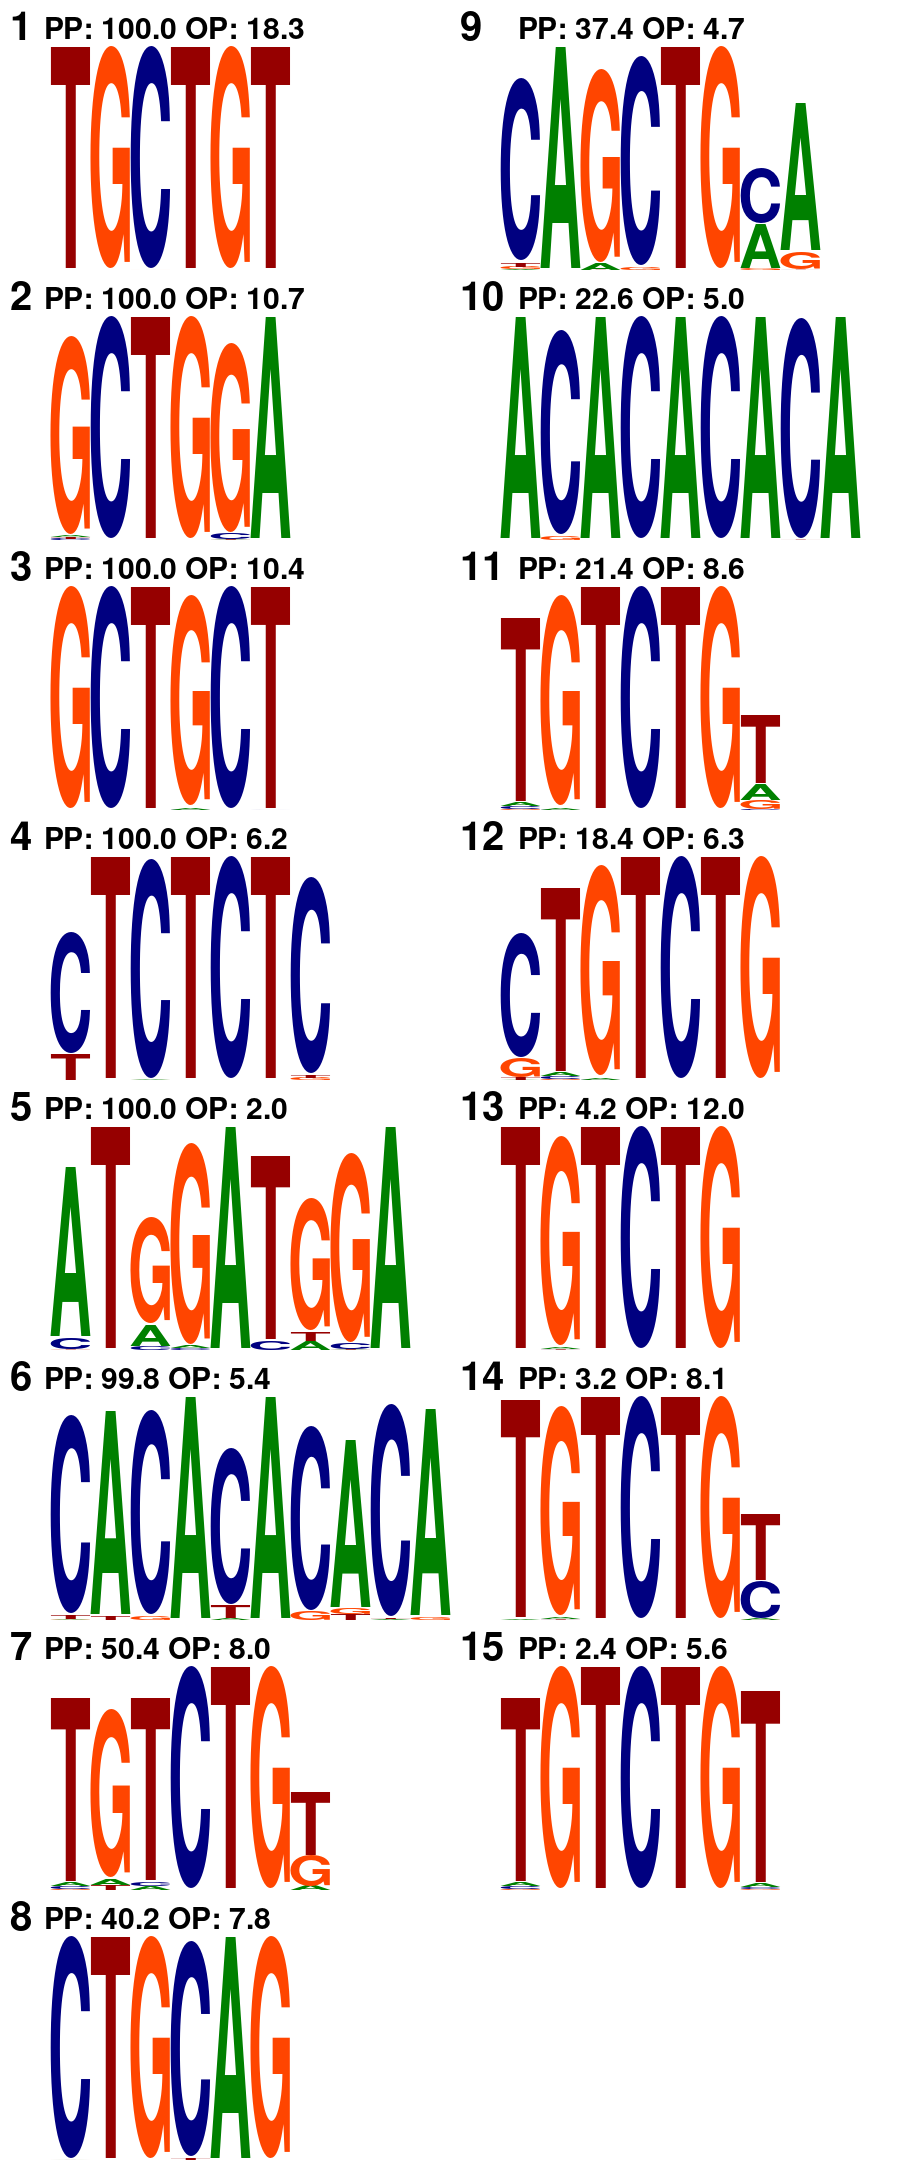
\includegraphics[width=.5\textwidth]{rys/sib_e_srcs.png}}    
    \caption{{\bf PWM sources detected in sibling differential nucleosome positions.}}
    PWMs presented as sequence logos with letter height proportional to position informational content\/emission probability.
    
    PP: Posterior prevalence; proportion of models within the compressed maximum a posteriori ensemble which have this PWM as a signal source

    OP: Observation prevalence; mean proportion of observed position sequences this sequence is used to explain, over all posterior samples
    \label{sibmotifs}
\end{figure}

\begin{figure}[!h]
    \makebox[\textwidth][c]{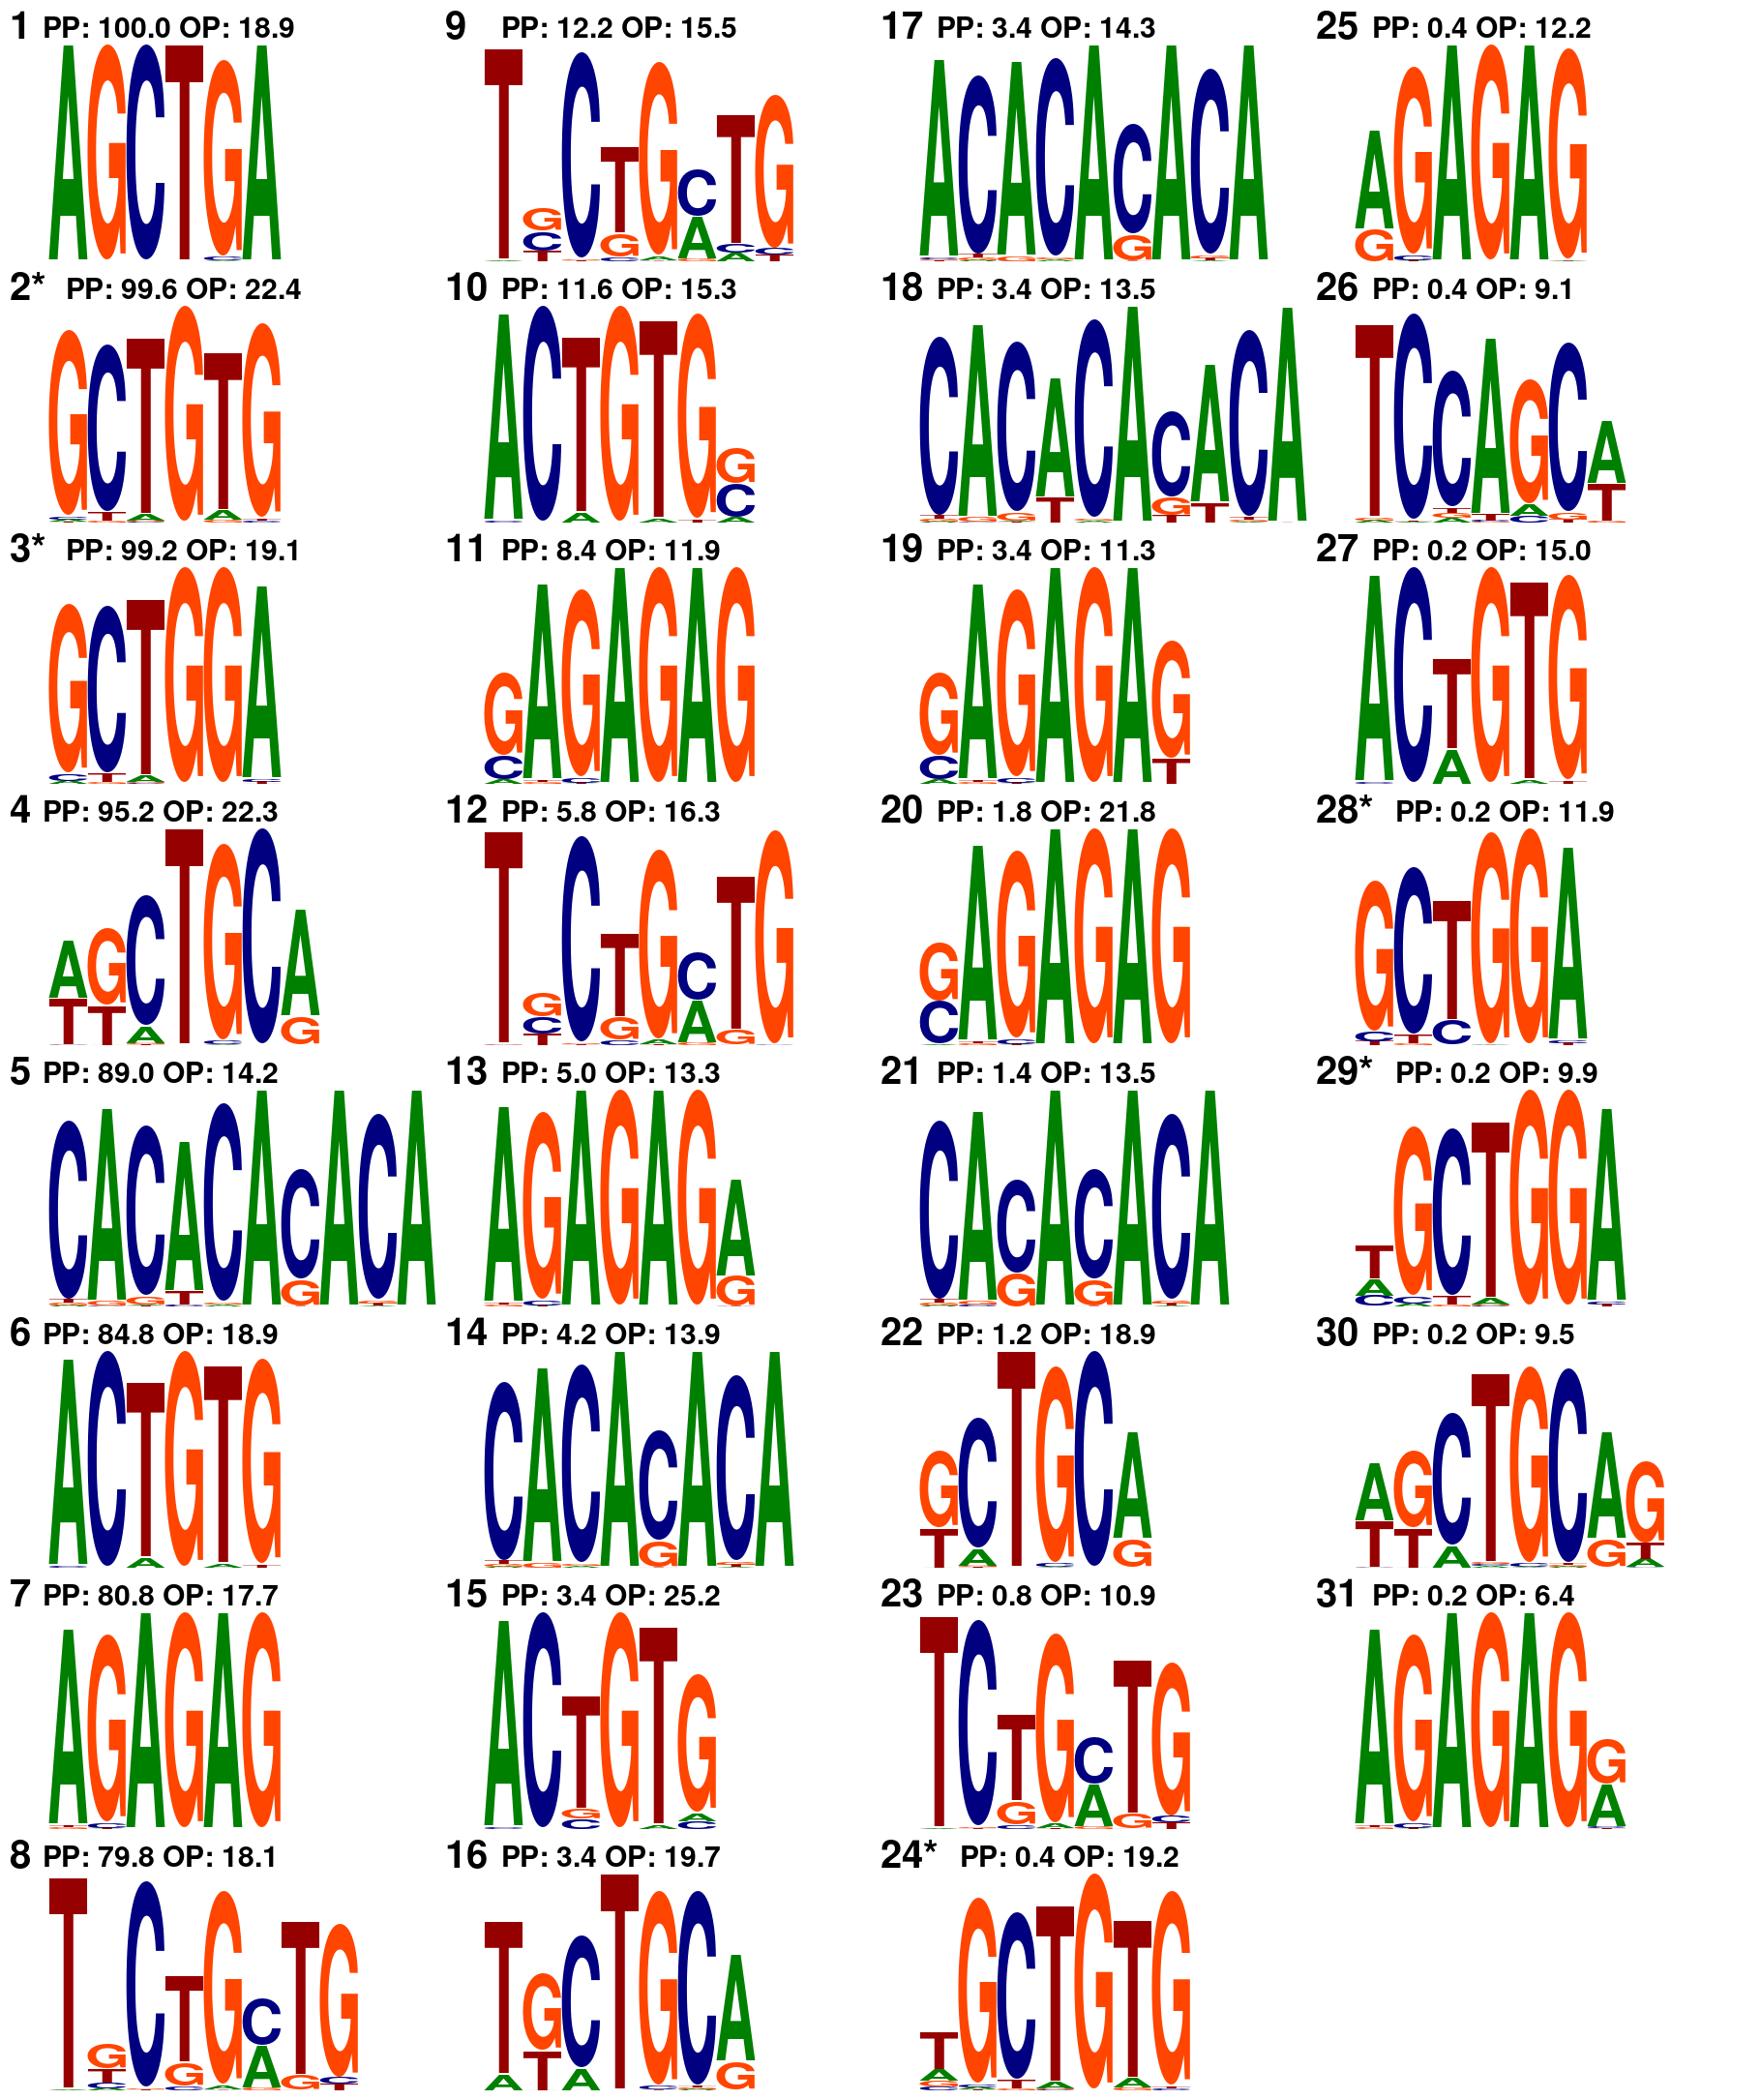
\includegraphics[width=1.\textwidth]{rys/rys_e_srcs.png}}    
    \caption{{\bf PWM sources detected in \textit{rys} mutant differential sources.}}
    PWMs presented as sequence logos with letter height proportional to position informational content\/emission probability.
    
    PP: Posterior prevalence; proportion of models within the compressed maximum a posteriori ensemble which have this PWM as a signal source

    OP: Observation prevalence; mean proportion of observed position sequences this sequence is used to explain, over all posterior samples
    \label{rysmotifs}
\end{figure}

\FloatBarrier

\section{Discussion}
We began our investigations by adding depth to the original description of the \textit{rys} mutant CMZ phenotype; on the basis of these investigations, we believe that a revision is in order. At any given time, the apparently increased size of the CMZ in \textit{rys}, relative to siblings, is produced as an effect of one or more of the following phenomena:

\begin{enumerate}
\item\label{inapret} Inappropriately retained RPCs in animals older than 7dpf
\item\label{specfail} Reduced neural population of the specified central retina, relative to the CMZ
\item\label{chromo} Expanded and spread-out RPC nuclei
\end{enumerate}

The first two effects are consistent with a failure of RPCs to specify as particular retinal neural lineages. This is substantiated by the inappropriate retention of early progentior markers in these cells. We demonstrate that \textit{rys} RPCs are not, however, arrested in cell cycle. In contradistinction to results finding elevated polyadenylated histone transcript levels associated with cell cyle arrest \cite{Kari2013}, we find that the mitotic activity of these cells actually accelerates under an overabundance of polyadenylated H2A and H2B transcript. We therefore suggest that the \textit{rys} phenotype is best characterised by chromatin disorganisation (phenomenon \ref{chromo}) and a failure of RPCs to correctly specify (which covers phenomena \ref{inapret} and \ref{specfail}) as retinal neural subtypes. The enlarged appearance of the CMZ is a result of these effects, and not a general increase in the CMZ population, RPC cytoplasmic volume\footnote{That is, by itself, without an increase in nucleus size. We did not directly measure this parameter.}, or other variables. 

Moreover, in identifying npat as the lesioned gene underlying the \textit{rys} phenotype, we nominate a general, well-evidentiated macromolecular mechanism underlying phenomenon \ref{chromo} which could plausibly produce phenomena \ref{inapret} and \ref{specfail}. That is, the mutant npat's effects on cell-cycle dependent histone transcription and stability may result in abberrant nucleosome positioning within proliferating cells, by altering the pool of histone proteins available for nucleosome formation. We posit that this is what causes the observed loss of a subpopulation of sibling nucleosome positions in \textit{rys}, together with the gain of novel, abberant positions. When we investigated whether the sequences of these subpopulations were better modelled by separate emissions processes than a combined emissions process, we found substantial evidence in favour of separate emissions processes. Interestingly, the PWM signals we detected in this differential nucleosome position set suggest some detail as to how changes in histone expression might result in the observed nuclear disorganisation of \textit{rys}. The observation that the background models explain the positions unique to siblings better than those unique to mutant \textit{rys} strongly suggests that sequence preference is less important in the process generating sibling positions than in the one generating mutant positions.

The relative importance of primary sequence in nucleosome positioning has been hotly debated; some have advocated for a nucleosome positioning code intrinsic to primary sequence \cite{Kaplan2009}, while others have disavowed the existence of any such code \cite{Zhang2009}. In general, the nucleosome dynamics community has moved on from these discussions in favour of emphasis on rotational sequence preferences \cite{Tolstorukov2007} and translational nucleosome positioning by \textit{trans}-acting factors \cite{Klages-Mundt2018}; a common interpretation of the earlier debate is that sequence preferences tend to dominate only at limiting concentrations of histones, when chromatin formation is rare \cite{Pointner2013}. The fact that sequence preference is less explanatory for the sibling positions than for the mutant ones is highly suggestive against this background. It seems likely that the shifted and novel nucleosome positions observed in mutants reflects all of the following:

\begin{enumerate}
    \item The appearance of nucleosomes with aberrant subunit composition
    \item A loss of translational control over \textit{rys} mutant nucleosomes by \textit{trans}-acting factors
    \item The limiting concentration of aberrantly-expressed nucleosomes, resulting in increased influence of ``default'' sequence-preference positioning
\end{enumerate}

All of the above could plausibly be caused by perturbed histone expression arising from altered npat activity. As the spatiotemporal dynamics of chromatin architecture are known to be critically involved in both replication timing \cite{Gilbert2010} and cell identity and fate \cite{Serrano2013}, the significant alterations we observe in \textit{rys} mutant chromatin architecture also provide a plausible molecular mechanism by which mutated npat protein can produce the observed shift in proliferative activity and failure of RPCs to specify, via altered histone expression. Moreover, chromatin density has recently been specifically implicated as fundamentally involved in the process by which pluripotent cells restrict gene expression to achieve their stable specified fates \cite{Golkaram2017}; it seems to be this overall process which has been disrupted in mutant \textit{rys}.

It is possible that the sequence-level inference is compromised by the ad-hoc nature of the sampler used to compress the ICA ensembles in our nested sampling procedure. For reasons explained in \autoref{ch:BMI}, the ICA model structure makes euclidean space representations difficult, and ensuring sampling is in detailed balance may not be possible, given changing PWM signal lengths. We suggest that it is appropriate to magnify our error estimate by several of magnitude as a consequence. If we concede that there are perhaps 5 orders of magnitude more error than estimated, this has the effect of reducing the significance of the result from to standard deviations, which is still well above the typical 5$\sigma$ significance typically accepted as a discovery in the physical sciences. We conclude that even given a more conservative estimate of the sampling processes' error, it is far more likely that the differential nucleosome populations found in \textit{rys} mutants and their phenotypically normal siblings are the result of separate generative processes. It is also possible that our identification of the differential subset of nucleosome positions with the disordered chromatin present in \textit{rys} RPCs is inaccurate. We have not conducted a full survey of \textit{rys} proliferative niches, and it is not clear how widely affected other cell types might be. Still, within the retina, only proliferative cells seem to have the chromatin phenotype, and it is on this basis that we make the identification, which is the most parsimonious available. 

There are a number of important lacunae in this explanation; it remains unclear what form of the npat protein is expressed, if any, as well as what the overall effect on the expressed pool of histones in RPCs is, for instance. It would not be very surprising if there are a number of macromolecular species intimately invovled in the \textit{rys} pathology which intermediate between the npat lesion and the observed chromatin phenotype which we have not examined. We suggest, however, that the overall effect on specification must be due to a failure of RPCs to organize chromatin for specification, and that, interestingly, this failure does not prevent proliferation. \textit{rys} therefore presents a useful model of the dissociability of proliferative and specificative behaviours in neural progenitors, which has recently been documented elsewhere in the developing \textit{D. rerio} retina \cite{Engerer2017}. Given the methodological limitations we encountered in probing protein expression in \textit{rys} RPCs, we suggest the most interesting and productive avenues of research to pursue in \textit{rys} pertain to this chromatin organisation phenotype.  Further experimentation is required to determine how specific changes in chromosome organisation (e.g. alterations in 3-dimensional chromatin organisation of gene expression, number of replication foci, etc.) produce specific features of the \textit{rys} phenotype. 

The zebrafish \textit{rys} mutant model provides a heretofore unique opportunity to study the role of a human NPAT homologue in a complete, developing tissue. This has previously proven difficult using mouse Npat, proviral inactivation of which resulted in early embryonic arrest, prior to tissue formation (Di Fruscio1997). The survival and development of \textit{rys} mutant embryos beyond this stage may reflect the presence of wild-type npat transcript contributed maternally \cite{Harvey2013}; \textit{rys} mutants nevertheless do not survive beyond metapmorhosis (\textasciitilde{}21dpf), so npat seems to be similarly obligatory for normal development in zebrafish, if over a longer timeframe. Still, we observed many differences between the function of npat in zebrafish and documented effects in other vertebrates, which require some explication.

As teleost fish are known to have undergone whole-genome duplication subsequent to their radiation from vertebrates, it is possible that zebrafish may have multiple npat paralogues. We have excluded this possibility due to our failure to identify any significantly similar CDS sequences in the Zv9 zebrafish genome using BLAST, and the synteny analysis in \autoref{synteny}. The zebrafish npat gene does have a substantially different genomic context from human NPAT, however: it is not associated with the eponymous ATM locus (which has been duplicated, and is present in this duplicate form elsewhere on chromosome 15). ATM’s 5’ position is, in zebrafish, occupied by hif1al, with the intergenic region lacking canonical E2F promoter sites. Of the 80 vertebrate genomes currently available from Ensembl, this organisation is shared only with the cave fish (A. mexicanus), with the human-like ATM-NPAT association preserved in all other species. This apparently evolutionarily novel genomic organisation for npat may be responsible for some of the differences in npat function we report here, relative to its homologues.

We identified alterations in histone mRNA transcription and 3’ end processing as likely mechanistically involved in the \textit{rys} phenotype. In both 6 and 8 dpf \textit{rys} larvae as well as npat-morpholino treated 1dpf embryos, we observe increased abundances of histone and, specifically, polyadenylated histone transcripts, although the composition of affected histone families differs between these contexts. The specific mechanism by which these effects are produced in \textit{rys} remains unclear, and the increases in histone transcript abundance observed in both mutant and morpholino-treated animals is at odds with observations that NPAT knockouts display decreases in histone transcription \cite{Ye2003}, and that the destruction of CDK phosphorylation sites on NPAT protein, which would be the case in the putatively truncated \textit{rys} npat protein, or treatment with a CDK inhibitor, result in similar declines in histone transcript abundance \cite{Ma2000,Mitra2009}. This may imply the role of zebrafish npat in regulating histone transcription is different from what has been described for human NPAT. We are unable to determine from these data whether the overall increases histone transcript abundance are a consequence of increased histone transcription, or of the greater stability of improperly polyadenylated histone transcript, however. The increased abundance of polyadenylated transcript in \textit{rys} mutants and npat morpholino-treated embryos is consistent with the observed role of NPAT in recruiting CDK9 to replication-dependent histone gene clusters, known to be important in generating the normal stem-loop structure at the 3’ end of these transcripts \cite{Pirngruber2009}, suggesting that this role is conserved in zebrafish. It is also possible that particular histone genes give rise to polyadenylated transcripts in zebrafish, as observed in a variety of cell lines \cite{Kari2013}; increased transcription of these particular genes might also account for the observed increase in polyadenylated histone transcript abundance. As noted above, although increased abundance of polyadenylated histone transcript has been associated with both cell cycle arrest and differentiation \cite{Kari2013}, we found that in the \textit{rys} mutant CMZ, this was associated with altered cell cycle parameters, failure to differentiate, and ultimately, cell death by apoptosis. This suggests that the presence of polyadenylated histone transcripts are not directly related to particular cell cycle states or differentiated fates, but rather that a particular regime of coordination and control of the expression of polyadenylated and replication-dependent, stem-looped histone transcripts is required to achieve appropriate transitions between these states. In the case of \textit{rys}, this seems to be related to the effect of altered histone expression on chromatin structure.
\chapter{Inferring and modelling specification dynamics in retinal progenitors}
\label{chap:rysoutro}

\section{Specification as a function of non-proliferative chromatin dynamics}
The npat mutant \textit{rys} investigated in \autoref{chap:rys} reinforces a basic theme running through this thesis, that lineage commitment or specification can be, and often is, dissociable from the proliferative behaviour of retinal progenitors, as has been suggested by Engerer et al. \cite{Engerer2017}. \textit{rys} illustrates this: RPCs undergo a final burst of proliferation before the death of the animal\footnote{Likely, on this view, arising from systemic failure of progenitors to specify appropriately.}, but never contribute appropriately to the neural retina. Indeed, older \textit{rys} larvae display a proliferative spillage of abberant RPCs into the intraocular space between the lens and GCL; the progeny of these abberant RPCs literally cannot be integrated into the tissue.

The importance of this dissociability for our inferences about RPCs can be gleaned from the basic problems encountered in each of the modelling studies. To begin with, the Stochastic Mitotic Mode Explanation models examined in \autoref{chap:SMME} failed, in large part, because the underlying Simple Stochastic Models conflate proliferation and specification under the ``mitotic mode'' concept. This leads immediately to the introduction of model structure to explain specification outside of ``mitotic mode'', assuming a phased temporal structure to RPC behaviour, without attempting to explain it. Lineage specification and niche exit processes need to be modelled separately from mitotic processes to differentiate their effects on outcomes. Next, proliferative data and morphological measurements in \autoref{chap:CMZ} fail to constrain the posterior distributions on the rate of niche exit in simple phased models, demonstrating that this parameter cannot be inferred with any certainty from overall population-level proliferative dynamics. To accurately model the behaviour of RPCs, data which provides accurate volumetric or temporal constraints on modelled specification or niche exit rate is of paramount importance. Finally, in \textit{rys}, we encounter the problem of explaining RPCs that proliferate but fail to specify; we explain this phenomenon in terms of the effects of mutant npat on chromatin organization by way of effects on histone expression. This directs us to the relevant level of organization for explanation of RPC lineage outcomes: the progression of chromatin states that underlay long-term changes in gene expression, which are required for the generation of the specified protein complement. Our  approach, while providing evidence for the chromatin dynamics we suggest arise from the effects of npat on the available histone pool, does not give us insight into how the appropriate progression of chromatin states might be usefully parameterised.

While a large number of techniques for studying aspects of chromatin structure exist, few suggest a means to describe an overall ``nuclear state''. That is, if we consider Waddington's idea of a cell's lineage state being a ball rolling down a canalized terrain \cite{Waddington1957}, it remains unclear what sort of parameter space would allow us to infer where the ball is. Older ideas of cellular state space, that rely exclusively on measures of protein expression, are unable to address hypotheses about chromatin structure. It remains unclear what aspects of chromatin organisation are causally important in fate commitment, as little formal model comparison has taken place. One might propose a joint structure-sequence-expression space with thousands of variables drawn from the vast literature on chromatin organisation. Such a project is unlikely to succeed with reasonable compute budgets, even with the sophisticated Bayesian inference tools developed here.

Still, if it is not obvious how one might build a general model of the evolution of ``nuclear state'', we may suggest some more limited approaches arising from the work presented in this thesis, that may make some headway here.

\section{Future directions}
\textit{rys} provides a useful platform for investigating the processes required to organize the progression of chromatin through the sequence of states we presume to be required for progression through the series of stages implied by the studies presented in \autoref{chap:SMME} and \autoref{chap:CMZ}, and the associated shifts in RPC lineage contributions. Despite the evidence amassed for the involvement of npat effects on nucleosome positioning in \textit{rys} mutants, many aspects of the suggested mechanism remain obscure. This arises, in part, from the lack of reliable macromolecular tools for investigating npat and histone proteins in \textit{D. rerio}. It would be useful to focus inquiry here on a small number of candidate histones. However, the large number of zebrafish histone genes, with no crystallographic data available, suggests that prediction of the involvement of particular histones would be difficult.

This situation is now rapidly changing, however. The AlphaFold algorithm has recently been recognized as a solution to the Critical Assessment of protein Structure Prediction (CASP) problem set in the CASP13 competition \cite{AlQuraishi2019}. This is the first time protein folding has been adequately predicted \textit{in silico} from sequence data alone. If it is possible to use this algorithm to predict \textit{D. rerio} nucleosome structures from histone folding predictions, this may obviate the need for crystallographic data. Such structural predictions could be used with the posterior estimates of signals putatively arising from nucleosome-DNA contact produced in \autoref{rysmotifs} to, in turn, predict which nucleosome compositions are most likely to favour the detected sequences. This might be assisted by 3d pattern matching for DNA sequences \cite{Herisson2007}, or roll-and-slide modelling of the contact motifs \cite{Tolstorukov2007} Such a study would produce hypotheses that, if interesting enough to pursue \textit{in vivo}, would supply estimates of how likely various histones are to be involved in the \textit{rys} mutant phenotype, and in what regard, which would help prioritise resources for the development of assays for interrogating the specific transcript and protein status of the most likely loci.

A more fundamental way of interrogating \textit{rys} ``nuclear state'' might be provided by focusing on transcription itself, which has been proposed as a primary driver of chromatin organisation \cite{Cook2018}. Such a project would likely require a transgenic line developed to monitor the transcription of one or more loci of interest in live cells, perhaps using bio-orthogonally labelled transcripts, as has recently been demonstrated in zebrafish \cite{Westerich2020}. This approach could possibly be used either to investigate the status and trafficking of npat and histone transcripts themselves, or to determine the impact of the npat lesion on the transcriptional shaping of chromatin organisation by tracking the transcription of progenitor markers, for instance.

Ultimately, it is likely that models that allow the prediction and control of RPC behaviour \textit{in situ} in zebrafish retinae will treat the chromatin organisation of RPC nuclei as an integrator of multiple relevant sources of information, including physical forces, cytoskeletal dynamics, and extracellular signals. This type of functional organisation, in which biological ``meaning'' arises from the integration of salient cellular information by a combination of nonarbitrary physicochemical relations and arbitrary biological coding reltaions, is currently best described by the subdiscipline of biosemiotics \cite{Hoffmeyer2008,Favareau2015,Hoffmeyer2015}. Of particular interest here is the clear-eyed and unobscurantist work of Marcello Barbieri, which may well provide the metaphysical framework necessary to plumb the depths of this topic \cite{Barbieri2014}.
\part{Software Technical Reports}
\chapter{GMC\_NS.jl}

\path{GMC_NS.jl} implements a basic Galilean Monte Carlo nested sampler \cite{Skilling2012} in pure Julia. It is not capable of multiprocess likelihood calculations like \path{BioMotifInference.jl} and is not intended for high-dimensional problems requiring dynamic ensemble size adjustment \cite{Higson2019} or multi-ellipsoidal sampling \cite{Feroz2009}. \path{GMC_NS.jl} accepts arbitrary user-defined functions for model calculations, so could be used for any moderately-sized sampling problem with a continuous parameter space.

\section{Implementation notes}

The basic sampling scheme followed is, first, to initialize an ensemble of models with parameters sampled evenly from across the prior, then to compress the ensemble to the posterior by applying GMC moves to the least-likely model in the ensemble at a given iterate, constrained by its current likelihood (which is the ensemble's likelihood contour for that iterate). GMC tends to move model-particles across the parameter space very efficiently, particularly in the initial portion of compression across the uninformative bulk of the prior mass. That said, GMC particles may get "stuck" in widely separated minima, so there are instances when the least-likely particle has no valid GMC moves. In this case, the trajectory is not continued. Instead, a new trajectory is begun by resampling from the remaining prior mass within the ensemble. This is accomplished by one of two means. Firstly, an attempt is made to resample by "diffusion". This means a random particle remaining within the ensemble is selected, and random velocity vectors are sampled from this particle to find a starting location for the new trajectory (this vector is conferred to the new particle). If diffusional sampling fails (extraordinarily rare), a primitive ellipsoidal sampler serves as a backup. This draws an ellispoid around the ensemble's current models in parameter space and samples evenly from the ellipsoid. While this is an acceptable method of sampling evenly from within the existing likelihood constraint, it is wildly inefficient for posteriors with any kind of interesting topology, which is both why multi-ellipsoidal sampling exists \cite{Feroz2009}, and why this single-ellipsoid sampler is confined to a backup role.

\path{GMC_NS.jl} follows the common convention of transforming parameter space to a unit-standardized hypersphere. The user is responsible for ensuring that the density of the prior is uniform, that is $\pi(x) = 1$, over the -1:+1 range of the hypersphere dimension. Utility functions \path{to_unit_ball} and \path{to_prior} which accept the prior and transformed positions and the relevant prior probability distribution, returning the unit hypersphere or prior coordinate, respectively. In future versions, this scheme is likely to be modified to a 0:1 unit hypercube, which does not require additional operations beyond obtaining the cumulative probability of a parameter value on the prior distribution. The user may also specify a sampling "box" to bound particles from illegal or nonsensical areas of the parameter space (eg. negative values for continuous distributions on positive-valued physical variables). The box reflects particles specularly in the same manner as the likelihood boundary, with the exception that because the orientation of the nth-dimensional box "side" is known (eg. is the plane at n=0.), the reflection is performed by stopping the particle at the box side and giving it a new velocity vector identical to the old but with reversed sign in dimension n. 

\path{GMC_NS.jl} attempts to maintain efficient GMC sampling by per-particle PID tuning of the GMC timestep. GMC treats models as particles defined by their parameter vectors, which give their positions in parameter space, as well as a velocity vector, normally chosen isotropically and only changed when the particle "reflects" off the ensemble's likelihood contour. In GMC, when a model-particle is to be moved through the parameter space (in this case, because it is the least likely particle in the ensemble), a new position is proposed by extending some distance along its velocity vector through the parameter space. This distance is determined by scaling the velocity vector by a "timestep" value, which can be thought of as the speed with which the particle is covering parameter space. As the model ensemble is compressed down to the posterior, this timestep must decline fairly evenly in order for GMC to be efficient, as the amount of available parameter space declines rapidly. Additionally, GMC particles may enter convoluted regions of parameter space that form small likelihood-isthmuses to other, more likely regions. In order to deal with this, each trajectory is assigned its own PID tuner, which maintains an independent timestep for the trajectory, tuned to target a user-supplied unobstructed move rate. In short, this will reduce the timestep if the particle is repeatedly reflecting off the likelihood boundary (in which case it is crossing the remaining prior mass without sampling much from it, or it is in a highly convoluted area of the local likelihood surface), and extend the timestep if it repeatedly moves without encountering the boundary, so that particles that are closely sampling an open region without encountering the boundary begin to "speed up". This scheme tends to produce a "shell" of swirling GMC particles reflecting obliquely off the likelihood contour, which gives good linear sampling of the entire likelihood range.

\section{Ensemble, Model, and Model Record interfaces}

\section{Usage notes}
\chapter{CMZNicheSims.jl: \textit{D. rerio} CMZ RPC niche simulators}
\label{chap:CNS}
\section{Introduction}
\path{CMZNicheSims.jl} (hereafter \path{CNS.jl}) comprises a set of three simulators of zebrafish retinal progenitor cells (RPCs), representing the postembryonic Circumferential Marginal Zone niche at varying levels of abstraction. These simulators were used in \autoref{chap:CMZ} and \autoref{chap:rys}. This package extends \path{GMC_NS.jl}, described in \autoref{chap:GMC}, and requires it. The simulators are organized around the nested sampling procedures implemented in that package. This means that simulations are executed as sample chains ("trajectories") from the simulations' parameter space in an ensemble. The basic operation of this package is accomplished by assembling an ensemble of models from the appropriate simulator submodule of \path{CNS.jl}, then elongating the trajectorie of this ensemble by Galilean Monte Carlo using \path{GMC_NS.jl}'s \path{converge_ensemble} function. Note that \path{GMC_NS.jl}'s sampler settings are specified by fields of the \path{CNS.jl} model ensemble struct and not as arguments to \path{converge_ensemble}; even if default sampler settings are used, sampler operation should be understood before model priors are selected.

The three model ensemble types specified by \path{CNS.jl} are as follows:

\begin{itemize}
    \item \protect\path{CMZ_Ensemble}: Phased difference function models of CMZ population and overall retinal volume, intended to model total retinal CMZ population and its contributions to overall retinal volume over long time periods (months)
    \item \protect\path{Slice_Ensemble}: Basic implementation of the ``slice model'' concept elaborated in \autoref{chap:SMMEoutro} for phased difference function CMZ models, uses a submodel of lens growth to determine ``out-of-slice'' growth contributions, intended to represent the population of a CMZ slice over long time periods (months)
    \item \protect\path{Thymidine_Ensemble}: ``Slice model'' of proliferative CMZ population exposed to a pulse of thymidine analogue, intended to model cell cycle kinetics in the CMZ over short time periods (hours). 
\end{itemize}

The operation of these simulators is described in more detail below. In general, the workflow is to assemble the assemble, converge it, and to estimate the model evidence and posterior parameters from the converged ensemble. For more on evidence and posterior estimation by \path{GMC_NS.jl}, see \autoref{chap:GMC}.

\section{\protect\path{CMZ_Ensemble} model and usage}
\label{sec:CMZmodel}
A \path{CMZ_Ensemble} consists of \path{CMZ_Model}s whose likelihood is assessed by \hyperref[ssec:MonteCarlo]{Monte Carlo} evaluation of a system of difference equations for simulated retinae, initialized from independent samples from the population and volume distributions specified in the ensemble constants vector. The update functions are specified in general by \autoref{popeq} and \autoref{voleq}. However, the implementation of these functions in the model likelihood function (\path{CMZ_mc_llh}, found in \autoref{ssec:CMZlh}) differs from this presentation; the equations are not evaluated stepwise day-by-day, but are rather updated for the next model event, either an observation timepoint or a phase transition date. The specific equations used in this function are of the computationally efficient factorial form suggested by Langtangen \cite[p. 559]{Langtangen2012}, so that the equation for the CMZ population $n$ days after some time 0 becomes:

\[
    p_n=p_{0} \cdot (2^{\frac{24}{CT}} - \epsilon)^{n}
\]

while the equation for retinal volume becomes:

\[
    v_n=v_{0} + p_{0} \cdot \epsilon \cdot \mu_{cv} \cdot \frac{1 - (2^{\frac{24}{CT} - \epsilon})^{n-1}}{1 - (2^{\frac{24}{CT} - \epsilon})}
\]

After Monte Carlo iterative simulation of many retinae, the resultant simulated population and volume distributions at the observed time points are estimated by fitting \path{LogNormal} \path{Distribution}s, after which the joint log likelihood of the observations given the simulation is calculated. The likelihood function is threaded so that the total number of Monte Carlo iterates for any given model parameter vector is divided equally between threads. For very large numbers of iterates, this can result in some load balancing inefficiency; in general, it is unneccessary to specify more than 5 million iterates in the ensemble constants vector (\autoref{constants} below). 1 million should be adequate for most purposes and allows the efficient sampling of $\geq$ 3 phase models on one performant machine.

A \path{CMZ_Ensemble} may be assembled by specifying the path of the folder in which its constituent model files will be serialized, the starting number of chains in the ensemble (a few thousand may reasonably be expected to converge within a day or two on a single high performance machine), the observations to estimate the models against, a vector of prior distributions, a vector of constants, a box matrix, and the sampler settings vectors. The parameter vectors must follow these guidelines:

\begin{enumerate}
    \item Observations vector: Must be a vector of vector tuples. The first member of the tuple is the population observation vector (total CMZ population at the vector's date index, see \ref{constants}), the second member is the date's total retinal volume observation vector (in \si{cubic}{micro}{meters}). Ie. the observations vector takes the form of a \path{AbstractVector{<:Tuple{<:AbstractVector{<:Float64},<:AbstractVector{<:Float64}}}}; the tuple of population and volume data found at index \path{x} corresponds from animals measured on date \path{constants_vec[1][x]}.
    \item Prior vector: For each desired phase of the model, the prior vector must contain a distribution over that phase's mean population cycle time (in hours) and its mean exit rate ($\geq$ 0., may exceed 1.). Paired cycle time and exit rate for each phase is followed by one less phase transition time in days than the number of phases. Ie. a two-phase prior vector might be, in pseudocode, \path{[Phase1CT, Phase1ER, Phase2CT, Phase2ER, Phase1End]}. 
    \item\label{constants} Constants vector: A \path{Vector{<:Any}} containing, in order:
    \begin{enumerate}
        \item T vector: Vector of integers or round floats, age in days of animals for each observations tuple
        \item Population distribution: \path{Distribution} defining the initial range of population values. Should normally be a fit from the initial population size observations
        \item Volume distribution:  \path{Distribution} defining the initial range of retinal volume values. Should normally be a fit from the initial retinal volume observations
        \item Monte Carlo iterates: Integer specifying the number of retinae to be simulated at each point sampled from the parameter space. \num{1e6}-\num{5e6} is usually fine.
        \item Phases: Integer defining the number of phases specified by the prior vector
    \end{enumerate}
    \item Box matrix: Two columns each of the same length as the prior, defining the minimum (column 1) and maximum (column 2) bounds for each parameter dimension to be sampled.
\end{enumerate}

As an example, an ensemble with 3000 chains and using the default GMC sampler settings may be initialized and sampled as follows, where variable names correspond to the vectors described above:

\begin{minted}[breaklines,
    mathescape,
    linenos,
    numbersep=5pt,
    frame=lines,
    framesep=2mm]{julia}
    e=CMZ_Ensemble(path, 3000, observations, prior, constants, box, GMC_DEFAULTS)
    converge_ensemble!(e,backup=(true,50), mc_noise=.3)
\end{minted}

The \path{mc_noise} parameter for \path{CNS.jl} models can be estimated by calculating the standard deviation of repeated evaluations of a parameter vector with a reasonably high likelihood, given the data vectors. The suggested value is roughly appropriate for \num{1e6} Monte Carlo iterates, given the data vectors used in \autoref{ssec:a10periodisation}.

\section{\protect\path{Slice_Ensemble} model and usage}
\label{sec:slicemodel}
A \path{Slice_Ensemble} consists of \path{Slice_Model}s, whose likelihood is assessed by \hyperref[ssec:MonteCarlo]{Monte Carlo} evaluation of a hybrid system of a difference equation and a power-law equation, representing a simulated CMZ RPC population in a retinal slice of arbitrary thickness. The \path{Slice_Model} likelihood function uses the same factorial solution to calculate the CMZ population after time steps of $n$ days as that described for \path{CMZ_Model}s. However, these population values are penalized by a value determined by using the power-law model of lens growth to determine the change in CMZ circumference over this time period, and the per-slice contribution required to expand the CMZ by this amount, given the present slice population and slice thickness (see \autoref{ssec:slicelensmodel} for this calculation).

\path{Slice_Model}s are broadly similar to \path{CMZ_Model}s. The parameter vectors required to assemble a \path{Slice_Ensemble} differ from those mentioned for a \path{CMZ_Ensemble}, however, and are summarised below. 

\begin{enumerate}
    \item Observations vector: Must be a vector of vector tuples. The first member of the tuple is the population observation vector (total CMZ population at the vector's date index, see \ref{constants}), the second member is the date's total retinal volume observation vector (in \si{cubic}{micro}{meters}). Ie. the observations vector takes the form of a \path{AbstractVector{<:Tuple{<:AbstractVector{<:Float64},<:AbstractVector{<:Float64}}}}; the tuple of population and volume data found at index \path{x} corresponds from animals measured on date \path{constants_vec[1][x]}.
    \item Prior vector: For each desired phase of the model, the prior vector must contain a distribution over that phase's mean population cycle time (in hours) and its mean exit rate ($\geq$ 0., may exceed 1.). Paired cycle time and exit rate for each phase is followed by one less phase transition time in days than the number of phases. Ie. a two-phase prior vector might be, in pseudocode, \path{[Phase1CT, Phase1ER, Phase2CT, Phase2ER, Phase1End]}. 
    \item\label{constants} Constants vector: A \path{Vector{<:Any}} containing, in order:
    \begin{enumerate}
        \item T vector: Vector of integers or round floats, age in days of animals for each observations tuple
        \item Population distribution: \path{Distribution} defining the initial range of population values. Should normally be a fit from the initial population size observations
        \item Lens model:  \path{Lens_Model} defining the lens circumferential growth power law and the slice's sectional thickness.
        \item Monte Carlo iterates: Integer specifying the number of retinae to be simulated at each point sampled from the parameter space. \num{1e6}-\num{5e6} is usually fine.
        \item Phases: Integer defining the number of phases specified by the prior vector
    \end{enumerate}
    \item Box matrix: Two columns each of the same length as the prior, defining the minimum (column 1) and maximum (column 2) bounds for each parameter dimension to be sampled.
\end{enumerate}

\section{\protect\path{Decay_Ensemble} model and usage}
\label{sec:decaymodel}
\path{Decay_Model}s are \path{Slice_Model}s that are parameterised to represent a continuous process of cell cycle rate decay (that is, lengthening cycle times). They use identical \path{Lens_Model}s to abstract the effects of the stretching 3-dimensional retina on the CMZ slice. Unlike the phased \path{CMZ_Model}s and \path{Slice_Model}s, \path{Decay_Model}s are parameterised solely by an initial cycle time $CT_{i}$, an exponential decay constant $\kappa$, and a constant exit rate $\epsilon$. Daily cycle time is evaluated as $CT_{t}=CT_i*e^{\kappa \cdot t}$. This is used to update the population value by the \path{Slice_Model} difference equation, penalized by the exit rate for the amount of CMZ growth implied by the \path{Lens_Model}.

A \path{Decay_Ensemble} is identical to a \path{Slice_Ensemble} except that it has only the three parameters in the order mentioned, and the corresponding prior vector, and omits the Phases constant.

\section{\protect\path{MultiSlice_Ensemble} model and usage}
A \path{MultiSlice_Model} consists of more than one slice observations set which are governed by identical parameter vectors. This allows independent observations from different areas of the CMZ to be collectively modelled by one \path{Slice_Model} or \path{Decay_Model} parameter vector. This can be used to represent a CMZ with morphological asymmetry but regulatory homogeneity, and is used as an alternative to separate models of morphologically distinguished slices in \autoref{chap:CMZ}. 

A \path{MultiSlice_Ensemble} is parameterised identically to the corresponding \path{Slice_Ensemble} or \path{Decay_Ensemble}, except that a vector of per-slice observations subvectors, and a vector of per-slice population distribution is provided. The \path{MultiSlice_Model} uses the paired observations and population distributions in vector order to build a vector of the appropriate slice model type, of the same length.

\section{\protect\path{Thymidine_Ensemble} model and usage}
\label{sec:thymidinemodel}
Unlike the population-level models described above, the \path{Thymidine_Model} is a cell-based lineage simulator. It retains the slice model concept of comparing simulated observations directly to counts obtained from cryosections. Because these counts are obtained over a short time period (1 day), no effort is made to account for the growth of the eye. It uses an explicitly modelled cell cycle with G1, S, and G2\/M phases.

The model assumes a LogNormal distribution of overall cell cycle lengths. It is parameterised by $TC_{\mu}$ and $TC_{\sigma^{2}}$ values for this LogNormal distribution (a \hyperref[ssec:normalgamma]{Normal Inverse Gamma prior} should be used), a fraction $s$ which gives the length of S-phase by multiplying into the sampled $TC$, a fraction $g1$, which gives the fraction of the remaining time which comes before S-phase as G1, and implies the length of the G2\/M phase afterwards. Finally, the fraction $sis$ is randomly added to or subtracted from the cell cycle length determined for one sibling of a mitosis to give the cell cycle length of the other. This represents the correlated sibling cell cycle times which characterise \textit{Danio} RPC populations, as usefully observed and modelled by He et al. \cite{He2012}. The parameter vector is given in the order \path{[tc$\mu$, tc$\sigma^{2}$, g1_frac, s_frac, sis_frac]}.

The model assumes linear labelling of nuclear contents over the cell cycle, and implements a minimum value for detection as a thymidine-labelled cell (\path{DETECTION_THRESHOLD}, set to .15 by default). This represents cells with a dusting of thymidine signal that are not counted as labelled, which normally occurs in confocal stack segmentation routines.

To simulate more than one subpopulation with independent cycle parameters, additional sets of the 5 parameters outlined above can be concatenated, with this vector appended by a parameter denoting the fraction of the population to which each additional parameterisation applies.

The \path{Thymidine_Ensemble} is constructed similarly to the other models, except that it requires a constants vector as follows:

Constants vector: A \path{Vector{<:Any}} containing, in order:
\begin{enumerate}
    \item T vector: Vector of integers or round floats, chase time in hours from beginning of pulse for each observations subvector
    \item Pulse: Float giving the length of the thymidine pulse in hours
    \item Monte Carlo iterates: Integer specifying the number of retinae to be simulated at each point sampled from the parameter space. \num{1e5}-\num{5e5} usually gives sufficient density over the discrete distribution to avoid noise associated with simulated count values that were not observed at all.
    \item End time: Float defining how long to run the simulation- should usually be the time of the last set of observations
\end{enumerate}

Unlike the population-level models, which fit LogNormal distributions to samples of output collected by Monte Carlo execution, the \path{Thymidine_Model} constructs discrete nonparametric distributions of simulated counts of labelled cells. This allows the model parameters to produce population distributions that diverge from smooth, continuous distributions. This is particularly notable in the banding pattern of some output, where some counts are very unlikely to be observed. This can allow the model to better reflect the prevalence of even-sized RPC lineages, for instance \cite{He2012}.
\chapter{BioBackgroundModels.jl}

\chapter{BioMotifInference.jl: Independent component analysis motif inference by nested sampling}
\label{chap:BMI}
\section{Introduction}
While many methods to detect overrepresented motifs in nucleotide sequences, only one is a rigorously validated system of statistical inference that allows us to calculate the evidence for these motif models, given genomic observations: nested sampling \cite{Skilling2006}. Computational biologists almost immediately benefitted from Skilling's original publication, with the release of the Java-coded nMICA by Down et al. in 2005 \cite{Down2005}. Unfortunately, this code base is no longer being maintained. It is, moreover, desireable to take advantage of modern languages and programming techniques to improve the maintainability and productivity of important bioinformatic code. We therefore re-implemented Skilling's original algorithm, for use in inference of DNA motifs in Julia \cite{Bezanson2015}, as \path{BioMotifInference.jl}, hereafter \path{BMI.jl}.

In brief, \path{BMI.jl} is intended to estimate the evidence for \hyperref[ICA]{Independent Component Analysis} models of \hyperref[PWM]{Position Weight Matrix} signals on \hyperref[HMM]{Hidden Markov Models} of genomic background noise, and to estimate the \hyperref[MAP]{maximum a priori} parameters of detected signals. This allows the user to perform Bayesian model selection and comparison for generative hypotheses about genomic sequences of interest.

\section{Implementation of the nested sampling algorithm}

Skilling's nested sampling algorithm is accompanied with an almost-certain guaranteed to converge an ensemble of models on the global optimum likelihood in the parameter space\cite{Skilling2006}. Skilling acknowledges an important assumption underpinning this guarantee, which is that the sampling density (in effect, the size of the ensemble) be high enough that widely separated modes are populated by at least one model each. Although early suggestions for the generation of new models within the ensemble were generally to decorrelate existing models by diffusional \hyperref[ssec:MonteCarlo]{Monte Carlo} permutation, later work generally acknowledges that this can be highly inefficient \cite{Skilling2012}, particularly in large parameter spaces with many modes, of which the sequence parameter spaces explored in \autoref{chap:rys} are good examples. A number of ways of addressing this problem have arisen in the cosmology and physics literature. These include improved sampling methods, such as sampling within an ellipsoidal hypersphere encompassing the positions of the ensemble models within the parameter space \cite{Feroz2008,Feroz2009} or Galiliean Monte Carlo (GMC) \cite{Skilling2012}, as well as methods of increasing computational efficiency, such as dynamic adjustment of ensemble size \cite{Higson2019}. 

Generally speaking, these methods are not good candidates for \path{BMI.jl} because the PWM representation of sequence signal in the ICA PWM model (IPM) is makes ordinary parameter space representation much less efficient. This is for at least four reasons:

\begin{enumerate}
    \item\label{identicalmodels} Identical IPMs may be expressed with their vector of PWM sources in different orders, so the parameter space becomes increasingly degenerate with higher numbers of sources.
    \item Closely equivalent repetitive signals can be represented by PWMs on opposite ends of the parameter space (e.g. ATAT vs TATA), reducing the efficiency of ellipsoidal sampling methods and introducing a further degeneracy.
    \item If model likelihoods are being calculated on the reverse strand of observations, sources on opposite ends of the parameter space (ie. reverse complements) can also represent closely equivalent signals, introducing another source of degeneracy.
    \item IPM sources may be of different lengths. Even if we can relate sources in different models to one another by some consistent distance rule, it is unclear how one would decide which dimensions of longer sources to project the parameters of shorter ones into. BioMotifInference does maintain an index for each source against its prior, but this is no guarantee that sources remain in some way "aligned". Rather, some type of alignment would have to be done, probably massively increasing computational cost to questionable benefit\footnote{Probably some combination of dimensional analysis and fast alignment algorithms could make some headway here, but it's not clear that it's necessary to do so.}.
\end{enumerate}

While it is possible to perform Markov Chain Monte Carlo in a manner that allows jumps between differently-dimensioned models in detailed balance, this applies only to diffeomorphic transformations \cite{Hastie2012}. PWM models are not merely matrices of unrelated parameters, but are an ordered sequence of 4-parameter discrete Categorical distributions. If the addition or removal of a discrete, indexed set of 4 parameters to an existing vector of such sets can be made reversible in this manner, the proof is beyond the scope of the present work\footnote{It is also likely to remain beyond my abilities. Please notify the author or submit a relevant pull request at \path{https://github.com/mmattocks/BioMotifInference.jl} if this is something you know how to do.}. Therefore, BioMotifInference (BMI) is not likely in strict detailed balance over a well behaved parameter space, given its default permute functions and configuration. Permute functions are designed around pragmatic concerns associated with the flow of model information in the IPM ensemble, and are tuned for computational efficiency in producing permuted models that are more likely than the starting model. Despite this, we show that its evidentiary accumulation behaviour strongly resembles that of a nested sampler that \textit{is} in detailed balance, suggesting that this problem is not fatal to the overall approach. Moreover, because of the extremely flexible nature of the sampler, the user may easily specify \path{BMI.jl}-compatible permute functions, should better ones for their application be apparent to them.

It should be noted that these considerations do not entirely preclude the operation of the \path{BMI.jl} in detailed balance over the prior. This can be achieved by the user specifying a single length for the PWM sources (rather than a range of permissible lengths), and using a permutation routine consisting solely of the functions \path{random_decorrelate} and \path{reinit_src}, along with any user-defined functions coded with the detailed balance stricture in mind. Operation in this fashion may improve the accuracy of both evidence estimates and the sources found in the maximum a posteriori (MAP) sample defined by the converged ensemble. That said, unless the supplied prior is unusually good, this mode of operation is only well suited to very small observation sets, on the order of kilobases. With uninformative priors and good background models, the vast majority of sources sampled from the prior will be significant likelihood penalties relative to the background model alone. Performing nested sampling on such an ensemble by diffusional techniques, in good detailed balance, will usually fail to produce models more likely than the background model within any reasonable compute budget, and will generally never converge. This feasibility constraint justifies the use of bespoke sampling routines for genome-scale datasets.

Like its predecessor \path{nMICA}, \path{BMI.jl} samples new models by applying one of a collection of permutation functions to an existing model. Additionally, although \path{BMI.jl} is supplied prior distributions on IPM parameters from which the initial ensemble is sampled, there is no way provided to calculate a posterior from the models generated by the nested sampling process, largely because of the identical source issue, \ref{identicalmodels}. The primary outputs of interest are the estimation of the Bayesian evidence for model structure given the data, given as its logarithm, as well as the models in the final ensemble (which constitute samples from the MAP mode or modes).

Because the more conventional methods to address the inefficiency of nested sampling by Monte Carlo used in cosmological models described above are unavailable, \path{BMI.jl} uses an ad hoc method of adjusting the mixture of permute patterns that are applied to models. The basic permute logic (encoded by \path{Permute_Instruct} arguments to the \path{permute_IPM} function) is as follows:

\begin{enumerate}
    \item\label{selectmodel} Select a random  model from the ensemble.
    \item\label{applyfunc} Apply a randomly selected permutation function from the instruction's function list according to the probability weights given to the functions by the instruction's weight vector.
    \item Repeat \ref{applyfunc} until a model more likely than the ensemble contour, given observations, is found, or the instruction's \path{func_limit} is reached.
    \item If the \path{func_limit} is reached without a new model being found, return to \ref{selectmodel} and repeat \ref{applyfunc} until a model more likely than the ensemble's contour is found, or until the instruction's \path{model_limit} is reached.
\end{enumerate}

\section{Usage notes}
\subsection{Preparation of observation set}
\path{BMI.jl} relies on \path{BioBackgroundModels.jl} both for selecting appropriate background models for motif inference, as well as to code observations and prepare an appropriate matrix of background scores. The selection of background models is covered in \autoref{chap:BBM}. The coding of observations requires the construction of a \path{DataFrame} containing a column of type \path{Vector{LongSequence{DNAAlphabet{2}}}}, the unambiguous DNA alphabet of \path{BioSequences.jl}. This is accomplished as follows:

\begin{minted}[breaklines,
    mathescape,
    linenos,
    numbersep=5pt,
    frame=lines,
    framesep=2mm]{julia}
    using BioBackgroundModels, DataFrames, Serialization
    obspath=/path/to/observations_dataframe
    obs_df=deserialize(obspath)
    coded_obs=observation_setup(obs, order=0, symbol=:seq)\end{minted}

Note that \path{observation_setup} must be supplied an \path{order} keyword argument of 0; while \path{BMI.jl} supports background HMMs of any order, signal motifs are 0\textsuperscript{th} order. If the name of the sequence column of the observations \path{DataFrame} differs from ``Seq'', a symbol specifying the column name should be passed as the \path{symbol} keyword argument.

To construct the background matrix, the observations must be masked by partition, and the positional likelihoods of the sequences calculated:

\begin{minted}[breaklines,
    mathescape,
    linenos,
    numbersep=5pt,
    frame=lines,
    framesep=2mm]{julia}
    BioBackgroundModels.add_partition_masks!(obs_df, genome_gff_path, 500, (:chr,:seq,:start))

    BHMM_dict = Dict{String,BHMM}()
    reports_folder=deserialize(/path/to/BBM_Reports_Folder)
    for (partition, folder) in reports_folder
        BHMM_dict[partition]=folder.partition_report.best_model[2]
    end

    background_scores=BGHMM_likelihood_calc(obs_df, BHMM_dict, symbol=:seq)\end{minted}

\path{add_partition_masks!} adds a mask column to the observations \path{DataFrame}, which is used by \path{BGHMM_likelihood_calc} to determine the correct background model to use for any given base in the observations sequence. It requires a path to a valid GFF3 annotation file for the genome. In order for the observations to be masked correctly, a tuple of column names containing the scaffold ID the observation is found on\footnote{It must be ensured that this ID corresponds to the one used by the GFF3}, the sequence on the positive strand, and the start position of the sequence on the scaffold.

The calculation of background scores requires a \path{Dict} of \path{BBM.jl} background models keyed by the partition ID. In the example, this is constructed programmatically from a \path{Report_Folder}; see \autoref{chap:BBM} for the generation of these reports.

\subsection{\protect\path{IPM_Ensemble} assembly}
Once the coded observation set and the matrix of background scores are prepared, an \path{IPM_Ensemble} may be initialised by sampling from a prior. Priors must first be assembled. This process is executed as follows:

\begin{minted}[breaklines,
    mathescape,
    linenos,
    numbersep=5pt,
    frame=lines,
    framesep=2mm]{julia}
    num_sources=5
    source_length_range=3:10
    uninformative_mixing_prior=.1
    source_prior = BioMotifInference.assemble_source_priors(num_sources, Vector{Matrix{Float64}}())
    mix_prior = (falses(0,0), uninformative_mixing_prior)

    e = BioMotifInference.IPM_Ensemble(worker_pool, "/path/to/ensemble/", ensemble_size, source_prior, (falses(0,0), mixing_prior), background_scores, coded_obs, source_length_range, posterior_switch=true)
\end{minted}

Here, an uninformative prior is assembled for 5 sources. If we wanted to supply some PWM samples create informative Dirichlet priors from, these would be supplied in the vector of matrices passed as the second positional argument to \path{assemble_source_priors}. Informative priors are produced by multiplying the PWM values by a fixed weight, which may be passed as the keyword argument \path{wt}.

An uninformative prior is supplied for the mixing matrix. The prior tuple consists of an empty \path{BitMatrix}; if an informative prior is desired, the appropriate \path{BitMatrix} for the informative sources is passed instead. Sources for which no informative prior is supplied have their mix vectors sampled from a fractional floating point success rate prior. Here, the \path{uninformative_mixing_prior} is .1, meaning that an average of 10\% of observations will be initialized with each source.

Sampling and likelihood calculations may be performed in parallel by submitting a valid integer vector worker pool as the first positional argument ot \path{IPM_Ensemble}, or conducted by the master process if this is omitted. Passing \path{true} for the keyword argument \path{posterior_switch} will ensure that the least likely models, discarded from the ensemble during the sampling procedure, are collected as samples from the posterior distribution. This is \path{false} by default, as no rigorous method for estimating posterior distributions is available.

\subsection{Permute routine setup}
\label{ssec:adhoc}
In order to converge an assembled \path{IPM_Ensemble} by nested sampling, it is necessary to provide an initial \path{Permute_Instruct}, which determines sampler behaviour, and is tuned by the \path{Permute_Tuner} to prioritize permute functions which currently produce the largest positive particle displacements over the likelihood surface in parameter space, per computational time. Some application-specific tweaking is usually necessary. Depending on how the computation is to be parallelized, the weights assigned ot network-intensive functions by the tuner, in particular, may benefit from being clamped. In order to convey how to set up an initial \path{Permute_Instruct} successfully, notes regarding the operation of the stock permute functions on \path{ICA_PWM_Model}s (IPMs) is summarized below. In this discussion, ``premature homogenisation'' refers to the loss of sampling density in relevant parts of the posterior, so that the ensemble particles are trapped in some local optimum.

\begin{itemize}
    \item \path{permute_source}: randomly permutes a single source in the IPM by altering the PWM weights or changing the length of the source. Distributions for the frequency and size of these permutations may be supplied. If the size of the perturbations is small, and the frequency of length changes is set to 0., this function is useful for finding sources that are slightly more probable than the current ones.
    \item \path{permute_mix}: flip a random number of mix matrix positions. Retains flips that make observations more probable. If the range of flip moves is kept small, this is a useful function for ``polishing'' the mix matrix, particularly of models with highly probable sources. Effective throughout the sampling process.
    \item \path{perm_src_fit_mix}: as \path{permute_source}, but the permuted source is supplied with a new mix vector which mixes the source solely into observations that it makes more probable. Efficient and effective throughout the sampling process.
    \item \path{fit_mix}: checks each source against each observation, mixes only those sources that make the observation more probable in isolation. By far the most important permute during the early sampling process, since it can quickly move improbable models sampled from uninformative priors into the portion of the parameter space with likelihoods greater than the background model. In effect, this allows the extraction of maximum information about the data from the initial sampling process, which typically produces many widely divergent sources. This prevents premature homogenisation of the ensemble after extensive sampling below the background model likelihood, and subsequent distortions of evidence and maximum a posteriori parameter estimates.
    \item \path{random_decorrelate}: perform the operations of \path{permute_source} and \path{permute_mix} on the same model. This is an inefficient permute in general, but it is useful for introducing new sources during the early part of a sampling run, in particular, working to prevent premature homogenisation.
    \item \path{shuffle_sources}: copy the source PWM from another model in the ensemble, leaving the original mix matrix. This can be an effective permute early in the sampling process. It is network intensive.
    \item \path{accumulate_mix}: randomly select a source from the model to be permuted. From another model in the ensemble, select the source which is most similar to the one selected in the original model. Add the two mixvectors together, such that the original source is now mixed in to any observations in the second model that had the similar source. This is an extremely effective permute when the ensemble begins to have many similar sources in different models, and often is the best way to produce models more likely than those produced by \path{fit_mix}. Network intensive. This is sometimes the last permute that can find model parameterisations more probable than those in a well-converged ensemble. Network intensive.
    \item \path{distance_merge}: Randomly select a source from the model to be permuted. From another model in the ensemble, select the most dissimilar source, and overwrite the selected source in the original model with the PWM and mixvector from this dissimilar source. This can be an effective permute throughout the sampling process. It tends to encourage the propagation of likely sources through the ensemble. Network intensive.
    \item \path{similarity_merge}: As \path{distance_merge}, except the most similar source is selected, and the original mixvector is retained. This tends to be less efficent than \path{distance_merge}, but can find new models throughout the sampling process. Network intensive.
    \item \path{reinit_src}: Resample a random source in the model to be permuted from the prior. This is a very inefficient permute, mostly useful in the early part of the sampling process to reintroduce sources from undersampled parts of the prior.
    \item \path{erode_model}: Trim a source's PWM in the model to be permuted to only those positions whose weight vectors express information above a threshold. This has the effect of generating high-likelihood short sources from longer ones with stretches of uninformative postions. It is mostly useful in the early part of the sampling process.
    \item \path{info_fill}: For a random source in the permute model, find the least informative PWM position, and set the probability of the most informative base to 1. This function assists in preventing premature homogenisation by rapidly increasing the likelihood of sources that are well-supported by observations but are unlikely to achieve appropriate high PWM weights by random permutation alone.
\end{itemize}

A \path{Permute_Instruct} requires a vector of the functions to be used in the permutation routine, a corresponding vector of their initial weights (ie. the frequency with which they will be called), a limit on the number of models to permute before the worker abandons sampling, and a limit on the number of functions to apply to any given model before selecting a new one to attempt permuting. The annotated example provided below also passes, as keyword arguments, vectors of minimum and maximum weights (\path{min_clmps} and \path{max_clmps}), as well as a vector of keyword arguments for the vector of functions (\path{args}).

\begin{minted}[breaklines,
    mathescape,
    linenos,
    numbersep=5pt,
    frame=lines,
    framesep=2mm]{julia}
    funcvec=full_perm_funcvec #exported by BMI.jl
    models_to_permute=10000
    func_limit=25
    
    #add two ``polishing functions'' to the function vector
    push!(funcvec, BioMotifInference.perm_src_fit_mix) 
    push!(funcvec, BioMotifInference.random_decorrelate)
    
    #all functions will receive a minimum of 1 in 100 function calls
    min_clamps=fill(.01,length(funcvec))

    #give some important functions a minimum of 10 in 100 function calls
    min_clamps[2:3].=.1 #perm_src_fit_mix & permute_mix
    min_clamps[8]=.1 #difference_merge

    #no function will receive more than 50 in 100 function calls
    max_clamps=fill(.5,length(funcvec))

    #prevent network intensive functions from swamping the cluster
    max_clamps[6:7].=.15 #shuffle_source and accumulate_mix
    max_clamps[9]=.15 #similarity_merge
    
    #evenly distributed initial weights
    initial_weights= ones(length(funcvec))./length(funcvec)
    
    #empty arguments vectors for all arguments in the funcvec
    args=[Vector{Tuple{Symbol,Any}}() for i in 1:length(funcvec)]
    
    #add arguments for the ``polishing functions''
    args[end-1]=[(:weight_shift_freq,0.),(:length_change_freq,1.),(:length_perm_range,1:1)]
    args[end]=[(:iterates,50),(:source_permute_freq,.3),(:mix_move_range,1:10)]
    
    #instantiate the Permute_Instruct
    instruct = Permute_Instruct(funcvec, initial_weights, models_to_permute, func_limit;min_clmps=min_clamps, max_clmps=max_clamps, args=args)
\end{minted}

\subsection{Nested sampling of \protect\path{IPM_Ensemble}s}

If all of the above-described tasks are met, the \path{IPM_Ensemble} may be converged by nested sampling using the specified permutation routine. This can be performed in parallel; any number of permutation workers may be used. However, because the master process is responsible for disk access, many such workers performing permutation functions which frequently require the deserialization of other models in the ensemble (those noted as ``network intensive'' above) will rapidly reduce the computational efficiency of the cluster. This can be mitigated by clamping network intensive permute functions to a lower frequency of total function calls.

\path{BMI.jl} is supplied with a display system similar to, but less customisable than \path{GMC_NS.jl}. An example of display setup and nested sampling execution is presented below:

\begin{minted}[breaklines,
    mathescape,
    linenos,
    numbersep=5pt,
    frame=lines,
    framesep=2mm]{julia}

display_rotation=[true,10,1,[[:tuning_disp,:lh_disp,:src_disp],[:conv_plot,:liwi_disp,:ens_disp]]]

logZ = converge_ensemble!(e, instruct, worker_pool, backup=(true,25), tuning_disp=true, lh_disp=true, src_disp=true, disp_rotate_inst=display_rotation)
\end{minted}

% \section{Recovery of spiked motifs}
%supplementary materials
\part{Supplementary Materials}
%methods appendices
\chapter{Supplementary materials for \autoref{chap:SMME}}
\label{chap:SMMsupp}
\section{Materials and methods}
\subsection{Zebrafish husbandry}
Zebrafish used in this study were of a wild type AB genetic background. Embryos were derived from pairwise crossings. Larvae were collected upon crossing and held in a dark incubator at 28\textdegree C. At 1dpf, embryos were treated with 100$\mu$l of bleach diluted in 170ml of embryo medium for 3 minutes, rinsed and dechorionated. Embryo medium was changed at 3dpf. After this, all animals were maintained at 28\textdegree C on a 14-hour light/10-hour dark cycle (light intesity of 300 lux) in an automated recirculating aquaculture system (Aquaneering). Animals were reared using standard protocols\cite{Westerfield2000}. Fish were sacrificed by tricaine overdose at the appropriate timepoints indicated in the text. All animal experiments were performed with the approval of the University of Toronto Animal Care Committee in accordance with guidelines from the Canadian Council for Animal Care (CCAC).
 
\subsection{Proliferative RPC Histochemistry}
\subsubsection{Anti-PCNA histochemistry}
In order to assay the number of proliferating cells in zebrafish CMZs, we used anti-PCNA histochemical labelling, as PCNA is, in zebrafish, detectable throughout the cell cycle in proliferating cells. After sacrifice as described above, fish (or their razor-decapitated heads, in the case of fish older than 30dpf) were fixed in 1:9 37\% formaldehyde:95\% ethanol at room temperature (RT) for 30 minutes, followed by overnight incubation in a fridge at 4\textdegree C. Subsequently, the samples were removed from fix and washed 3 times in PBS. They were then cryoprotected by successive 30 minute rinses at RT on a rocker in 5\%, 13\%, 17.5\%, 22\%, and 30\% sucrose in PBS. Samples were allowed to incubate overnight at 4\textdegree C in 30\% sucrose. The next day, samples were removed from the sucrose rinse and infiltrated with 2:1 30\% sucrose:OCT compound (TissueTek) for 30 minutes at RT. Samples were then embedded for cryosectioning and frozen. 14$\mu$m coronal cryosections were cut through the fish's heads and collected on Superfrost slides (Fisherbrand). These were stored in a freezer at -20\textdegree C until staining.

Staining was begun by allowing the slides to dry briefly at RT. Sections were outlined with a PAP pen, then rehydrated in PBS for 30 minutes at RT. Subsequently, sections were blocked in 0.2\% Triton X-100 + 2\% goat serum in PBS for 30 minutes at RT. This was followed by incubation in mouse monoclonal (PC10) anti-PCNA primary antibody (Sigma), diluted 1:1000 in blocking solution, at 4\textdegree C overnight. The next day, primary antibody was removed, and slides were rinsed five times in PDT (PBS + 1\% DMSO + 0.1\% Tween-20). Cy5-conjugated goat-anti-mouse secondary antibody (Jackson Laboratories), diluted 1:100 in blocking solution, was applied to the sections, which were incubated at 37\textdegree C for 2 hours. Secondary antibody was removed, followed by five rinses in PDT as above. Sections were counterstained with Hoechst 33258 diluted to 100 $\mu$g/mL in PBS for 15 minutes at RT. Counterstain was then removed, five rinses in PDT were performed as above, followed by a final rinse in PBS. Slides were then mounted in ProLong Gold antifade mounting medium (ThermoFisher Scientific), coverslipped, and sealed with clear nail polish. Slides were kept at 4\textdegree C until imaging.

\subsubsection{Cumulative thymidine analogue labelling for estimation of CMZ RPC cell cycle length}
In order to obtain an estimate of cell cycle length in CMZ RPCs at 3dpf, we used cumulative thymidine analogue labelling following the method of Nowakowski et al.\cite{Nowakowski1989}. 3dpf zebrafish were divided into ten groups of n\=5 animals and held in 10 mM EdU for 0.5, 1.5, 2.5, 3.5, 4.5, 5.5, 7.5, 8.5, 9.5, and 10.5 hours, after which they were sacrificed as described above. Samples were processed as described under ``Anti-PCNA histochemistry", except that goat-anti-mouse Cy2-conjugated secondary antibody (Jackson Laboratories) was used to label anti-PCNA, after which the Alexa Fluor 647-conjugated azide from a Click-iT kit (ThermoFisher Scientific) was added to the sections for 30 minutes at room temperature to label EdU-bearing nuclei. This was followed by five PDT rinses as described above, and resumption of the protocol with counterstaining, mounting, etc. The raw data is available in \path{\empirical_data\cumulative_edu.xlsx}

\subsubsection{Whole retina thymidine analogue labelling of post-embryonic CMZ contributions}
We used thymidine analogue labelling as an indelible marker of CMZ contributions to the retina in Fig \ref{RingFig}. Because thymidine analogues are incorporated into DNA during S-phase, postmitotic progeny of proliferating RPCs which take up the label may be detected at any point after this treatment. Dosing zebrafish with a thymidine analogue for a limited period of time ensures that the label is diluted to undetectable levels in cells which continue to proliferate. Repetitive dosing thus gives rise to labelled cohorts which represent a limited set of generations of cells which become postmitotic after the dose is provided. n=3 fish were held in 10mM BrdU (Sigma) diluted in facility water for 8 hours at 30, 60, 90, 120, and 150 days post fertilisation. 10 days after the last BrdU incubation, the fish were sacrificed as described above. One representative whole retina dissection is presented.

\subsection{Confocal microscopy and image analysis}
All histochemically processed samples (coronal sections of retinas and whole retinas) were imaged on a Leica TCS SP5 II laser confocal imaging microscope, using the Leica LAS AF software for acquisition. For coronal sections, central sections were identified by their position in the ribbon of cryosections. For Fig \ref{WanSim}, the central section was imaged together with the flanking section on either side of it. Confocal data was analysed using Imaris Bitplane software (v. 7.1.0). Cell counting analyses were performed by segmenting the relevant channels using the Surfaces tool to produce counts of PCNA positive (Figs \ref{WanSim}, \nameref{cumulativeSupplement}) or PCNA/EdU double-positive (\nameref{cumulativeSupplement}) nuclei. Lens diameters were measured in the DIC channel using the linear measurement tools, across the widest point of the section of spherical lens.

\subsection{Estimation of CMZ annular population size}
\label{sec:lenspopest}
In order to estimate the total population of the CMZ in zebrafish eyes sampled throughout the first year of life, we counted PCNA-positive cells in the dorsal and ventral CMZ of central and flanking sections of these eyes as described above. We added the dorsal and ventral populations and took the average of the central and flanking section per-section populations to reduce the possibility of sampling error. We treated this as a sample of a torus mapped to the 14$\mu$m sphere segment of lens intersected by the average section. As the surface area of this zone is given by $S = \pi \times d_{lens} \times h_{section}$, and the total surface area of the lens by $A = \pi \times d_{lens}^2$, where $d$ is the diameter of the lens and $h$ the section thickness, we may calculate an estimate of the total population by $pop_{total} = \frac{pop_{section}}{S} * A$. We therefore obtained our annular CMZ population estimates using our measurements with the simplified formula $pop_{total}=\frac{pop_{section} \times d_{lens}}{h_{section}}$, calculating $pop_{total}$ on a per-eye basis to account for covariance of the measurements, and subsequently averaging across n=6 eyes per sampled timepoint (3, 5, 8, 12, 17, 23, 30, 60, 90, 120, 180, and 360 dpf). These data are presented in Fig \ref{WanSim}.

\subsection{Modelling lens growth}
To simulate the annular CMZ population, we wanted to be able to simulate the stem cells at the periphery of the retina occasionally undergoing symmetric divisions, so as to keep up the same density of stem cells in the first ring around the lens. We did this by normalising our lens diameter measurements to the 72hpf value, to produce a measure of relative increase in lens size over the first year of CMZ activity. We performed a linear regression of the logarithm of this relative increase vs the logarithm of time using the Python statsmodels library, using the constants derived from this regression for a power-law model of lens growth. This model was used to supply the \path{WanStemCellCycleModel} with a target population value as described below.

\subsection{Estimation of 3dpf CMZ cell cycle length}
To produce an estimate of the length of the cell cycle in 3dpf RPCs, we first took the total count of EdU-positive cells in dorsal and ventral CMZ from our cumulative labelling experiment described above, and divided by the total dorsal and ventral CMZ RPC population, as measured by the number of PCNA positive cells. This gave the labelled fraction measurements displayed in \nameref{cumulativeSupplement}. Following Nowakowski et al. \cite{Nowakowski1989}, we performed an ordinary least squares linear regression on these data using the Python statsmodels library. We then calculated the total cell cycle time $T_c = \frac{1}{slope}$ and $T_s = T_c \times intercept_y$. While this method is not suited for heterogenous populations of proliferating cells, its use is justified here, as the He SSM to which the estimate is being applied makes similar assumptions as Nowakowski et al., in particular the homogeneity of the population. It should not be considered more than a rough estimate.

\subsection{CHASTE Simulations}
\subsubsection{Project code}
All simulations were performed in an Ubuntu 16.04 environment using the CHASTE C++ simulation package version 2017.1 (git repository at \url{https://chaste.cs.ox.ac.uk/git/chaste.git}). The CHASTE package is a modular simulation suite for computational biology and has been described previously\cite{Mirams2013}. All of the code, simulator output, and empirical data used in this paper is available in the associated CHASTE project git repository at \url{http://github.com/mmattocks/SMME}, as well as in the supplementary archive \nameref{S1_File}. In brief, the approach taken was to encapsulate the SSMs examined here as separate concrete child classes inheriting from the CHASTE \path{AbstractSimpleCellCycleModel} class. An additional model, representing the simple immortal stem cell proposed in Wan et al.\cite{Wan2016}, was similarly produced. Each model is generic and provided with public methods to set their parameters and output relevant simulation outcomes (and per-lineage debug data, if necessary). While these may be used in the ordinary CHASTE unit test framework, permitting their use in any kind of cell-based simulation, we wrote standalone simulator executables (apps, in CHASTE parlance) to permit Python scripting of the simulator scenarios used in this study. This allows for the multi-threaded Monte Carlo simulations performed herein. Therefore, the Python fixtures available in the project's \path{python_fixtures} directory were used to operate the single-lineage simulators (\path{GomesSimulator}, \path{HeSimulator}, and \path{BoijeSimulator}) and single-annular-CMZ simulator (\path{WanSimulator}) in \path{apps/}, including the CellCycleModels and related classes in \path{src/}; the simulators output their data into \path{python_fixtures/testoutput/}. These data, along with the empirical observations (both from the Harris groups' papers and our own described herein) available in \path{empirical_data/}, were processed by the analytical Python scripts in \path{python_fixtures/figure_plots/} to produce all of the figures used in this study.

We have attempted to make the project fully reproducible and transparent. CHASTE uses the C++ boost implementation of the Mersenne Twister random number generator (RNG) to provide cross-platform reproducibility of simulations. All of our simulators make use of this feature, permitting user-specified ranges of seeds for the RNG. We have also used the numpy libary's RandomState Mersenne Twister container to provide reproducible results for the Python fixtures, notably the SPSA optimisation fixture. The output of the project code will, therefore, be identical every time it is run, on any platform.

It should be noted that none of the code Harris' group used in their reports has been published. We have made every effort to replicate the functional logic of the models as closely as possible. Nonetheless, it is not possible to determine precisely why, for instance, the original He SSM parameterisation failed so notably in our implementation.

\subsubsection{SPSA optimisation of models}
In order to make a fair comparison between the He SSM and our deterministic mitotic mode alternative model, we coded an implementation of the SPSA algorithm described by Spall \cite{Spall1998}. This is available in \path{/python_fixtures/SPSA_fixture.py}. This algorithm, properly tuned, will converge almost-surely on a Karush-Kuhn-Tucker optimum in the parameter space, given sufficient iterates, even with noisy output (eg. due to RNG noise from low numbers of Monte Carlo samples, permitting conservation of computational resources). It does so by approximating the loss function gradient around a point in parameter space, selecting two sampling locations at each iterate, then moving the next iterate's point in parameter space ``downhill" along this gradient.

 Our loss function was a modified AIC; we weighted the residual sum of squares from the PD-type mitotic probabilities by 1.5 in order to improve convergence, as the PD data are the most informative part of the dataset regarding the critical phase boundaries (PP mitoses occur in all 3 phases of the He model, DD occur in phases 2 and 3, PD mitoses occur only in phase 2). We also compared model induction count output (that is, panels A-C in Fig \ref{SDFig}) up to count values of 1000 to penalise parameters producing very large lineage totals.

 The values of the SPSA gain sequence constants were selected to be as large as possible without resulting in instability and failure to converge; this ensured that the algorithm stepped over the widest possible range of the parameter space in finding optima. The $\alpha$ and $\gamma$ coefficients were initially set at the noise-tolerant suggested values of .602 and .101 respectively \cite{Spall1998}. 200 iterations were performed. Initially, each iterate involved 250 seeds of each induction timepoint for the count data (panels A-C in Fig \ref{SDFig}) and 100 seeds of the entire 23-72 hr simulation time for mitotic mode rate data (panels D-F).  At iterate 170, these were increased to 1000 and 250 seeds, respectively, decreasing RNG noise to a low level. For the last 10 iterations, RNG noise was reduced to close to nil by increasing the seed numbers to 5000 and 1250, respectively; $\alpha$ and $\gamma$ were set to the asymptotically optimal 1 and $\frac{1}{6}$ for these iterates, as well. The particular seeds used were kept constant throughout in order to take advantage of the improved convergence rate this affords \cite{Kleinman1999}.
 
 Because the simple SPSA can assign any value to parameters, our implementation uses constraints, projecting nonsensical values for parameters (e.g. negative values, mitotic mode probabilities summing to $>1$) back into legal parameter space. The use of constraints has no effect on the algorithm's ability to almost-surely converge within the given parameter space\cite{Sadegh1997} As we felt that the deterministic mitotic mode models' ``sister shift" should be relatively small in order to be biologically plausible, we also constrained this parameter such that 95\% of sister shifts would be less than the mean length of the shortest phase.
 
 The numerical results of the SPSA algorithm are available in \path{/python_fixtures/testoutput/SPSA/HeSPSAOutput}, alongside png images of output from each iterate, enabling the visualisation of the progress of the algorithm.
 
\paragraph{Monte Carlo simulations}
 Subsequent to SPSA optimisation, the parameters derived from this procedure were used to perform Monte Carlo simulations of large numbers of individual lineages, using ranges of 10000 non-overlapping seeds for each of panels A, B, C, G, H, and I, and 1000 for each of panels D, E, and F of Fig \ref{SDFig} (using the SPSA-optimised parameter sets) and \nameref{originalSupplement} (using the original He et al. parameterisation). This was performed using \path{/python_fixtures/He_output_fixture.py}.
 
 Similarly, 100 seeds were used in Monte Carlo fashion to simulate individual annular CMZ populations using \path{/python_fixtures/Wan_output_fixture.py}, which scripts the WanSimulator. Each of these simulations is initialised with an RPC population drawn from a normal distribution given the mean and standard deviation of the CMZ torus estimated from our 3dpf observations, as described above. Each RPC is given a TiL value randomly chosen from 0 (newly born from a stem cell) to 17hr (exiting the CMZ, ``forced to differentiate", in the terms of Wan et al.). A further population of stem cells, sized at $\frac{1}{10}$ of the RPC population, is added using the \path{WanStemCellCycleModel}. This stem population divides asymmetrically except when it falls under its target population value determined by the model of lens growth described above; as long as this condition holds, the stem cells will divide symmetrically to keep up their numbers.
 
\paragraph{Simulation data analysis}
Not all of the numerical data used in He et al. and Wan et al. has been published. As such, we reconstructed the lineage data from He et al.'s Figure 5C, used by He et al. to obtain their mitotic mode probabilities; our reconstructed values are available in \path{/empirical_data/empirical_lineages\}. We also reconstructed the He et al. WT and Ath5 morpholino data (Fig \ref{SDFig} panels H, I) and Wan et al. lineage count probabilities (panel G) from the relevant figures. These values are entered into \path{/python_fixtures/figure_plots/He_output_plot.py}, where they are used in the AIC calculations described below. 

In order to assess the performance of the models used in our simulations, we used Akiake's Information Criterion (AIC). This allows us to compare models with dissimilar numbers of parameters, as AIC trades off goodness-of-fit against parameterisation. The values reported in Table \ref{AICtable} were produced by \path{/python_fixtures/figure_plots/He_output_plot.py}.

The 95\% CIs for the model output presented in this paper were estimated by repetitive sampling of the output data, using the same number of lineages observed empirically. 5000 such samples were performed. This provides a reasonable estimate of the confidence interval given the limited observational sample size.
 
\section{Supporting figures}

\begin{figure}[p]
\makebox[\textwidth][c]{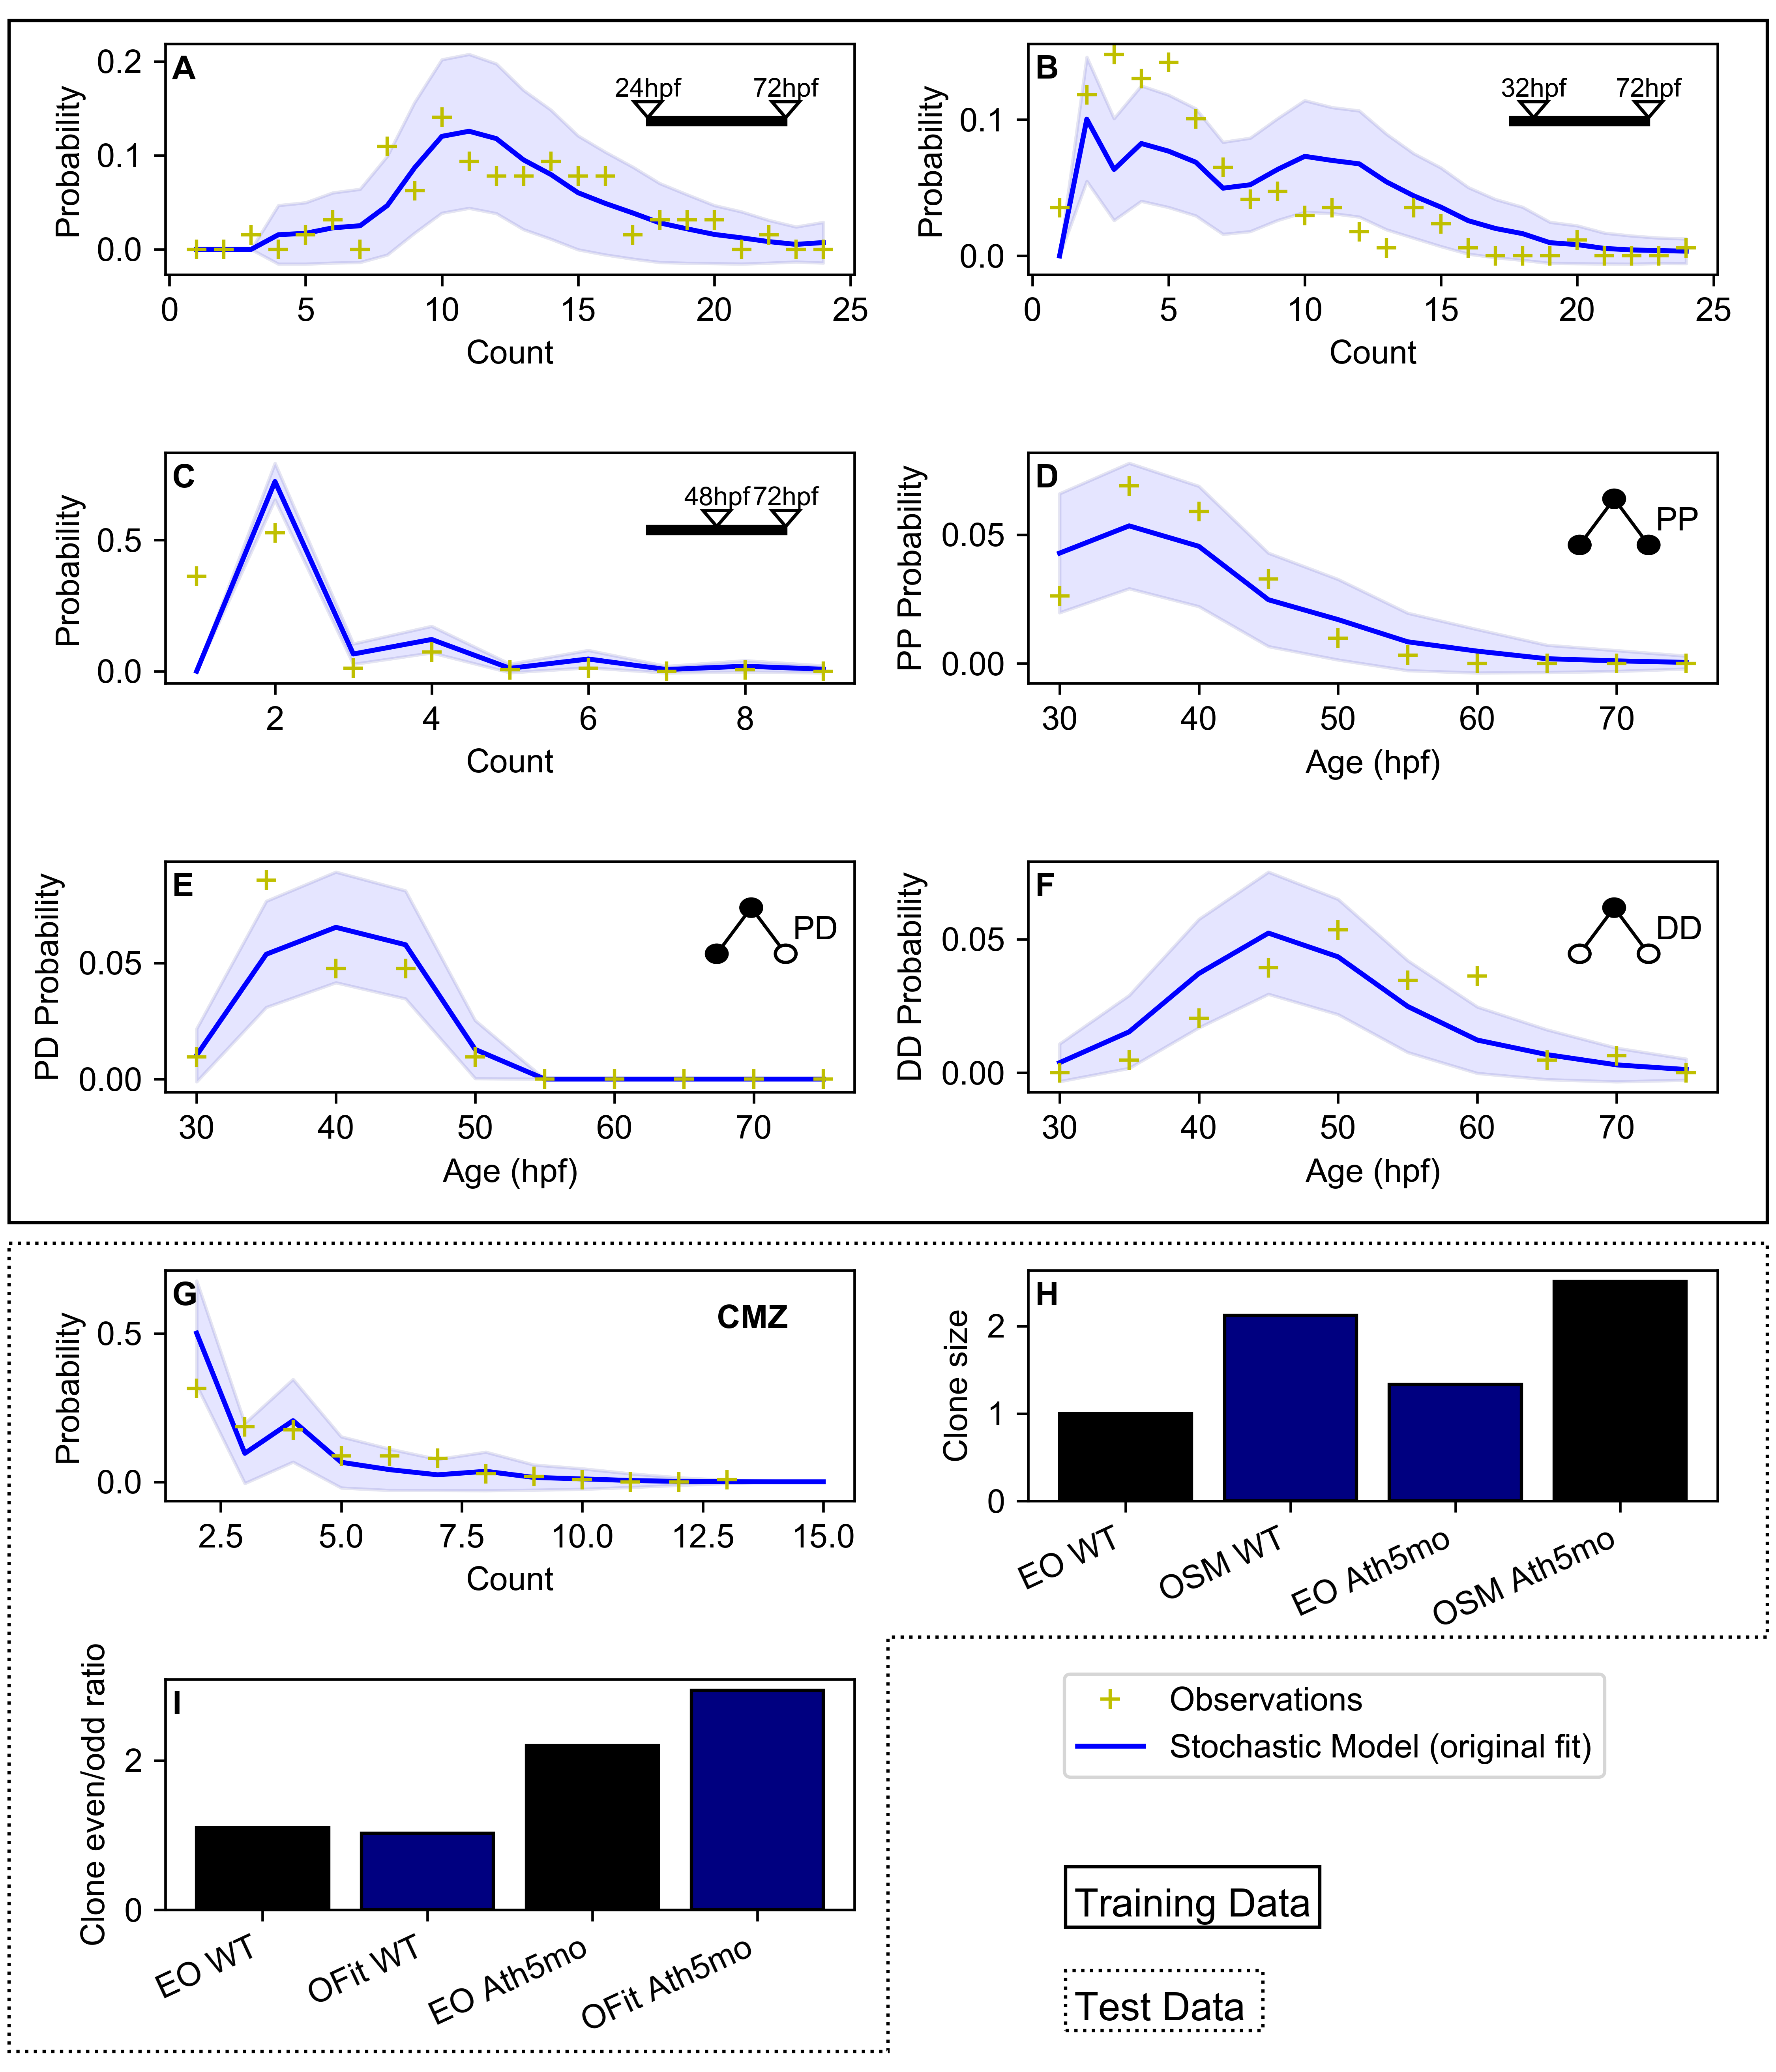
\includegraphics[width=1.\textwidth]{ssm/Fig_S1_o_fig.png}}
\paragraph{S1 Fig.}
\label{originalSupplement}
{\bf He SSM original parameterisation model output.} As Fig \ref{SDFig}; model output uses the parameterisation given in He et al.\cite{He2012}. Note significant deviation from observations in panel B, reflecting excess proliferative activity of modelled RPCs.
\end{figure}

\begin{figure}[p]
\makebox[\textwidth][c]{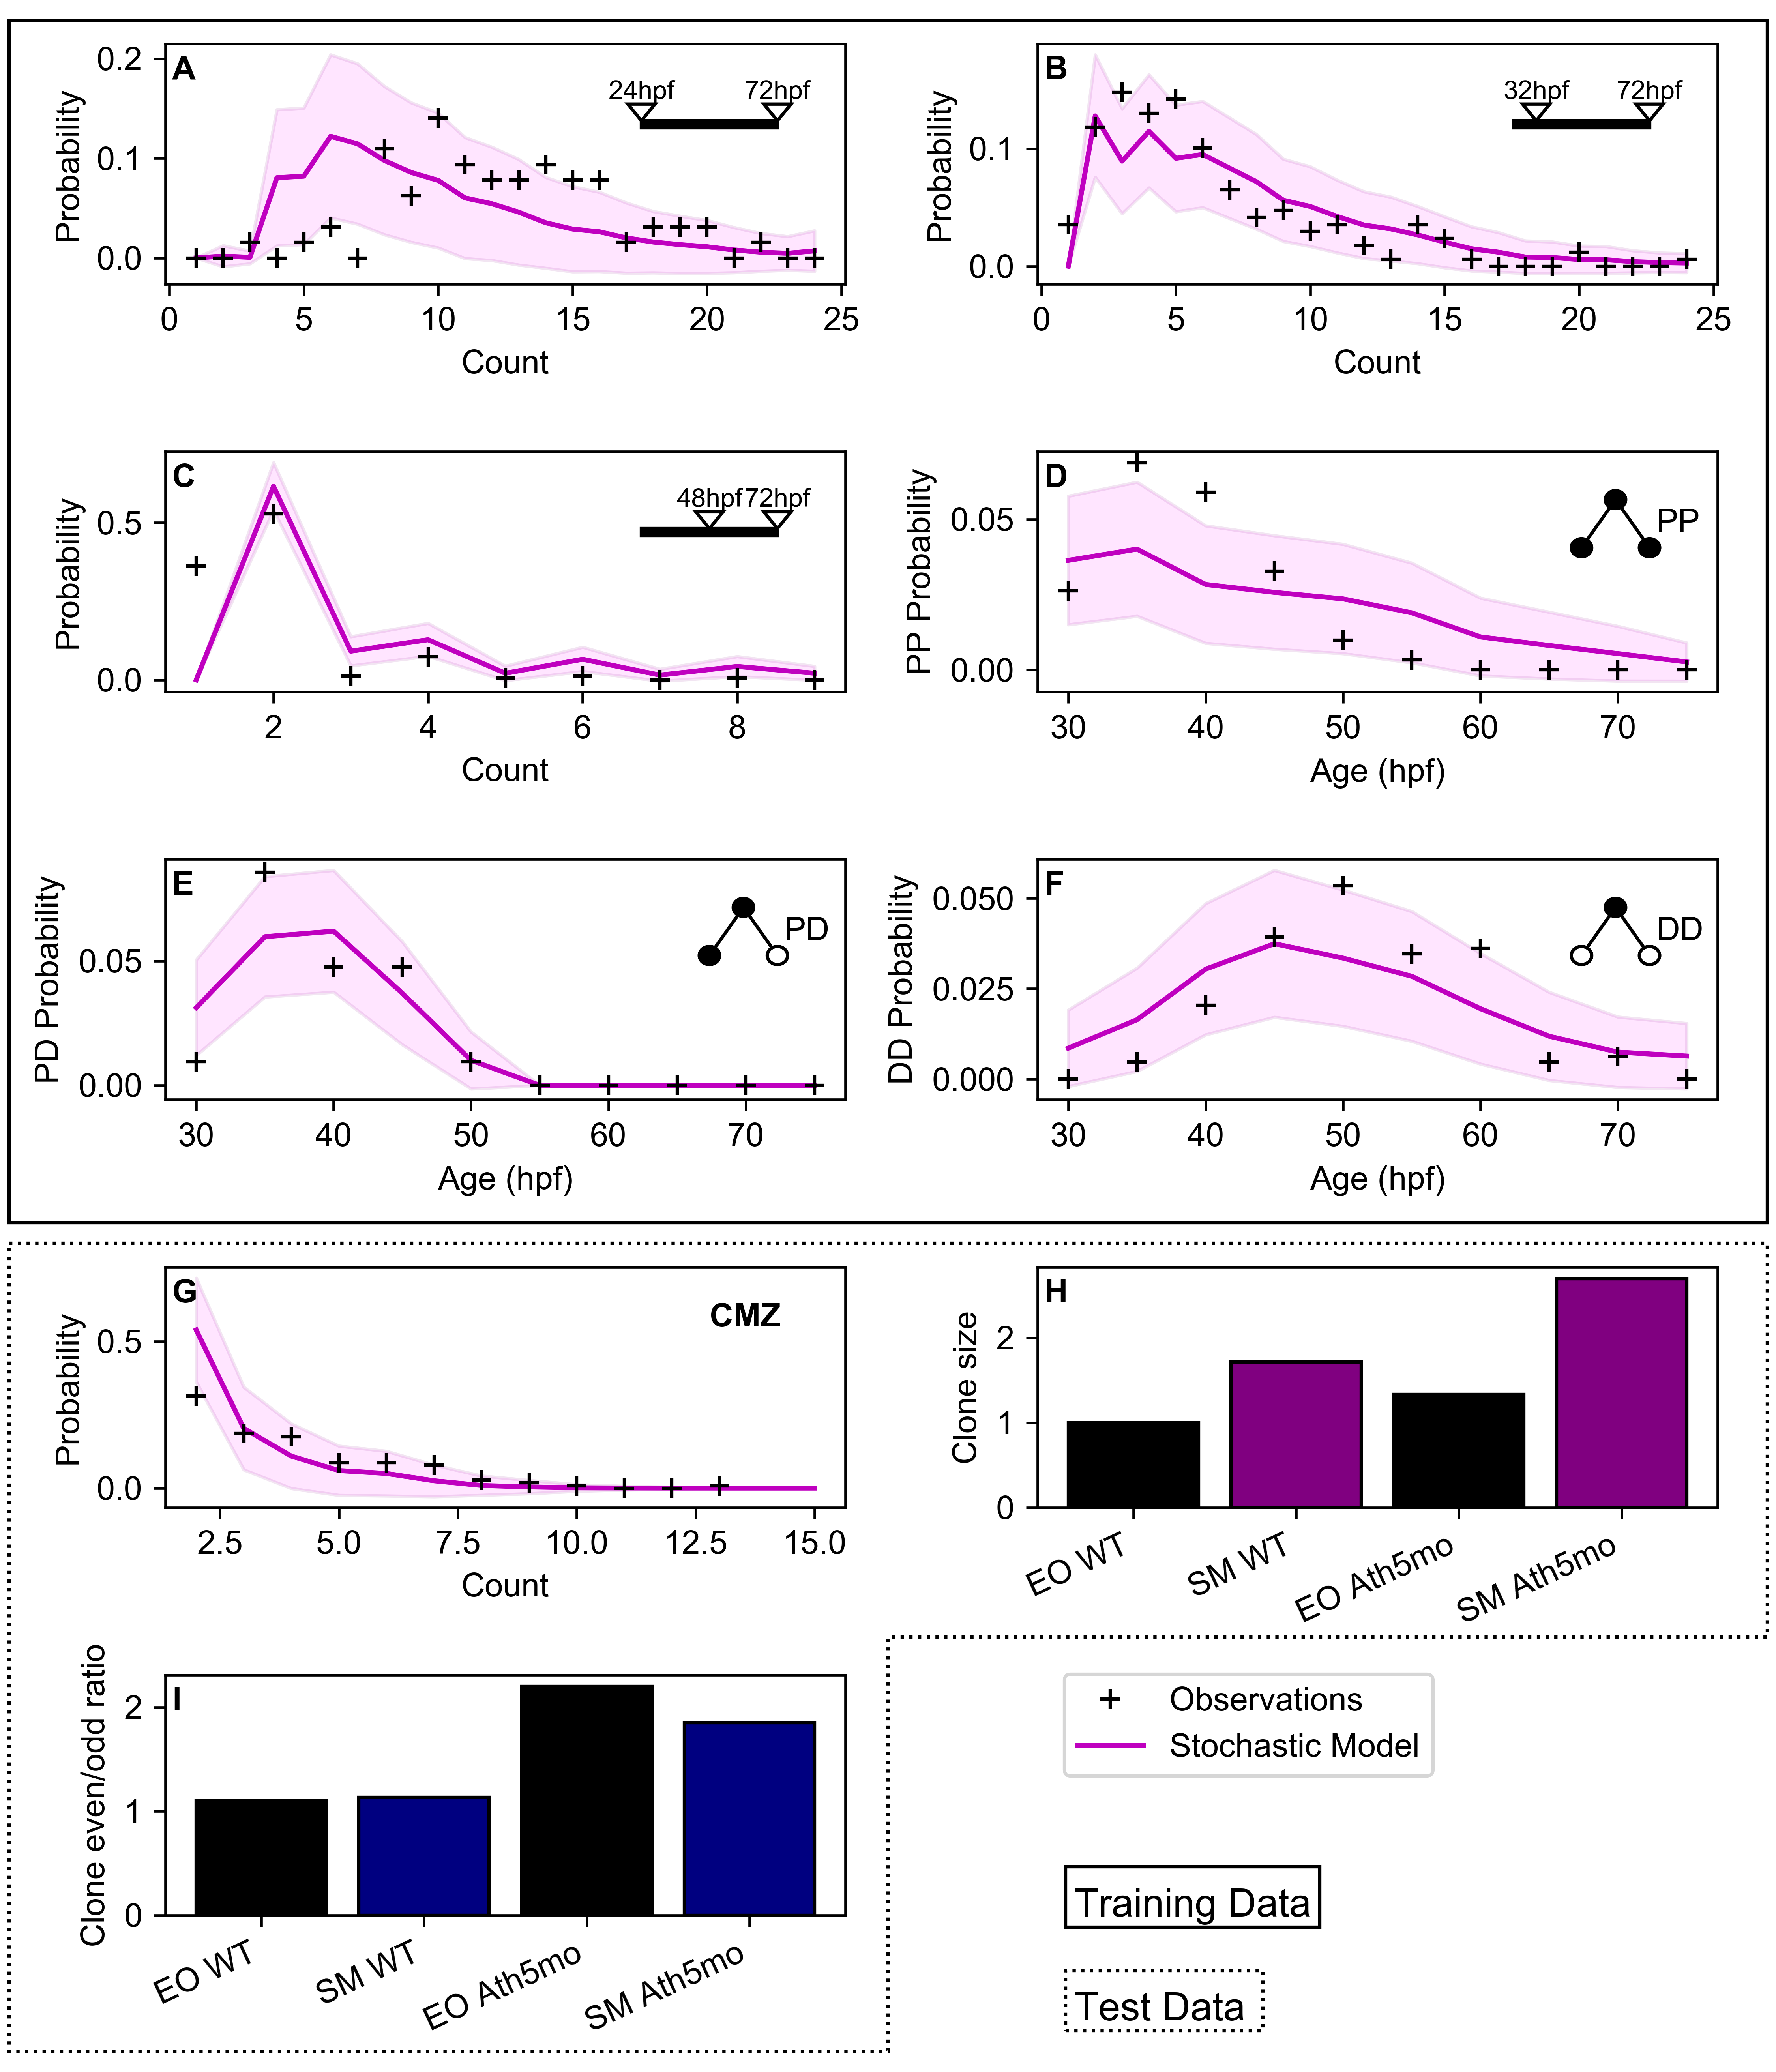
\includegraphics[width=1.\textwidth]{ssm/Fig_S2_s_fig.png}}
\paragraph{S2 Fig.}
\label{stochasticSupplement}
{\bf SPSA-optimised He SSM model output.} As Fig \ref{SDFig}; stochastic model output displayed alone.
\end{figure}

\begin{figure}[p]
\makebox[\textwidth][c]{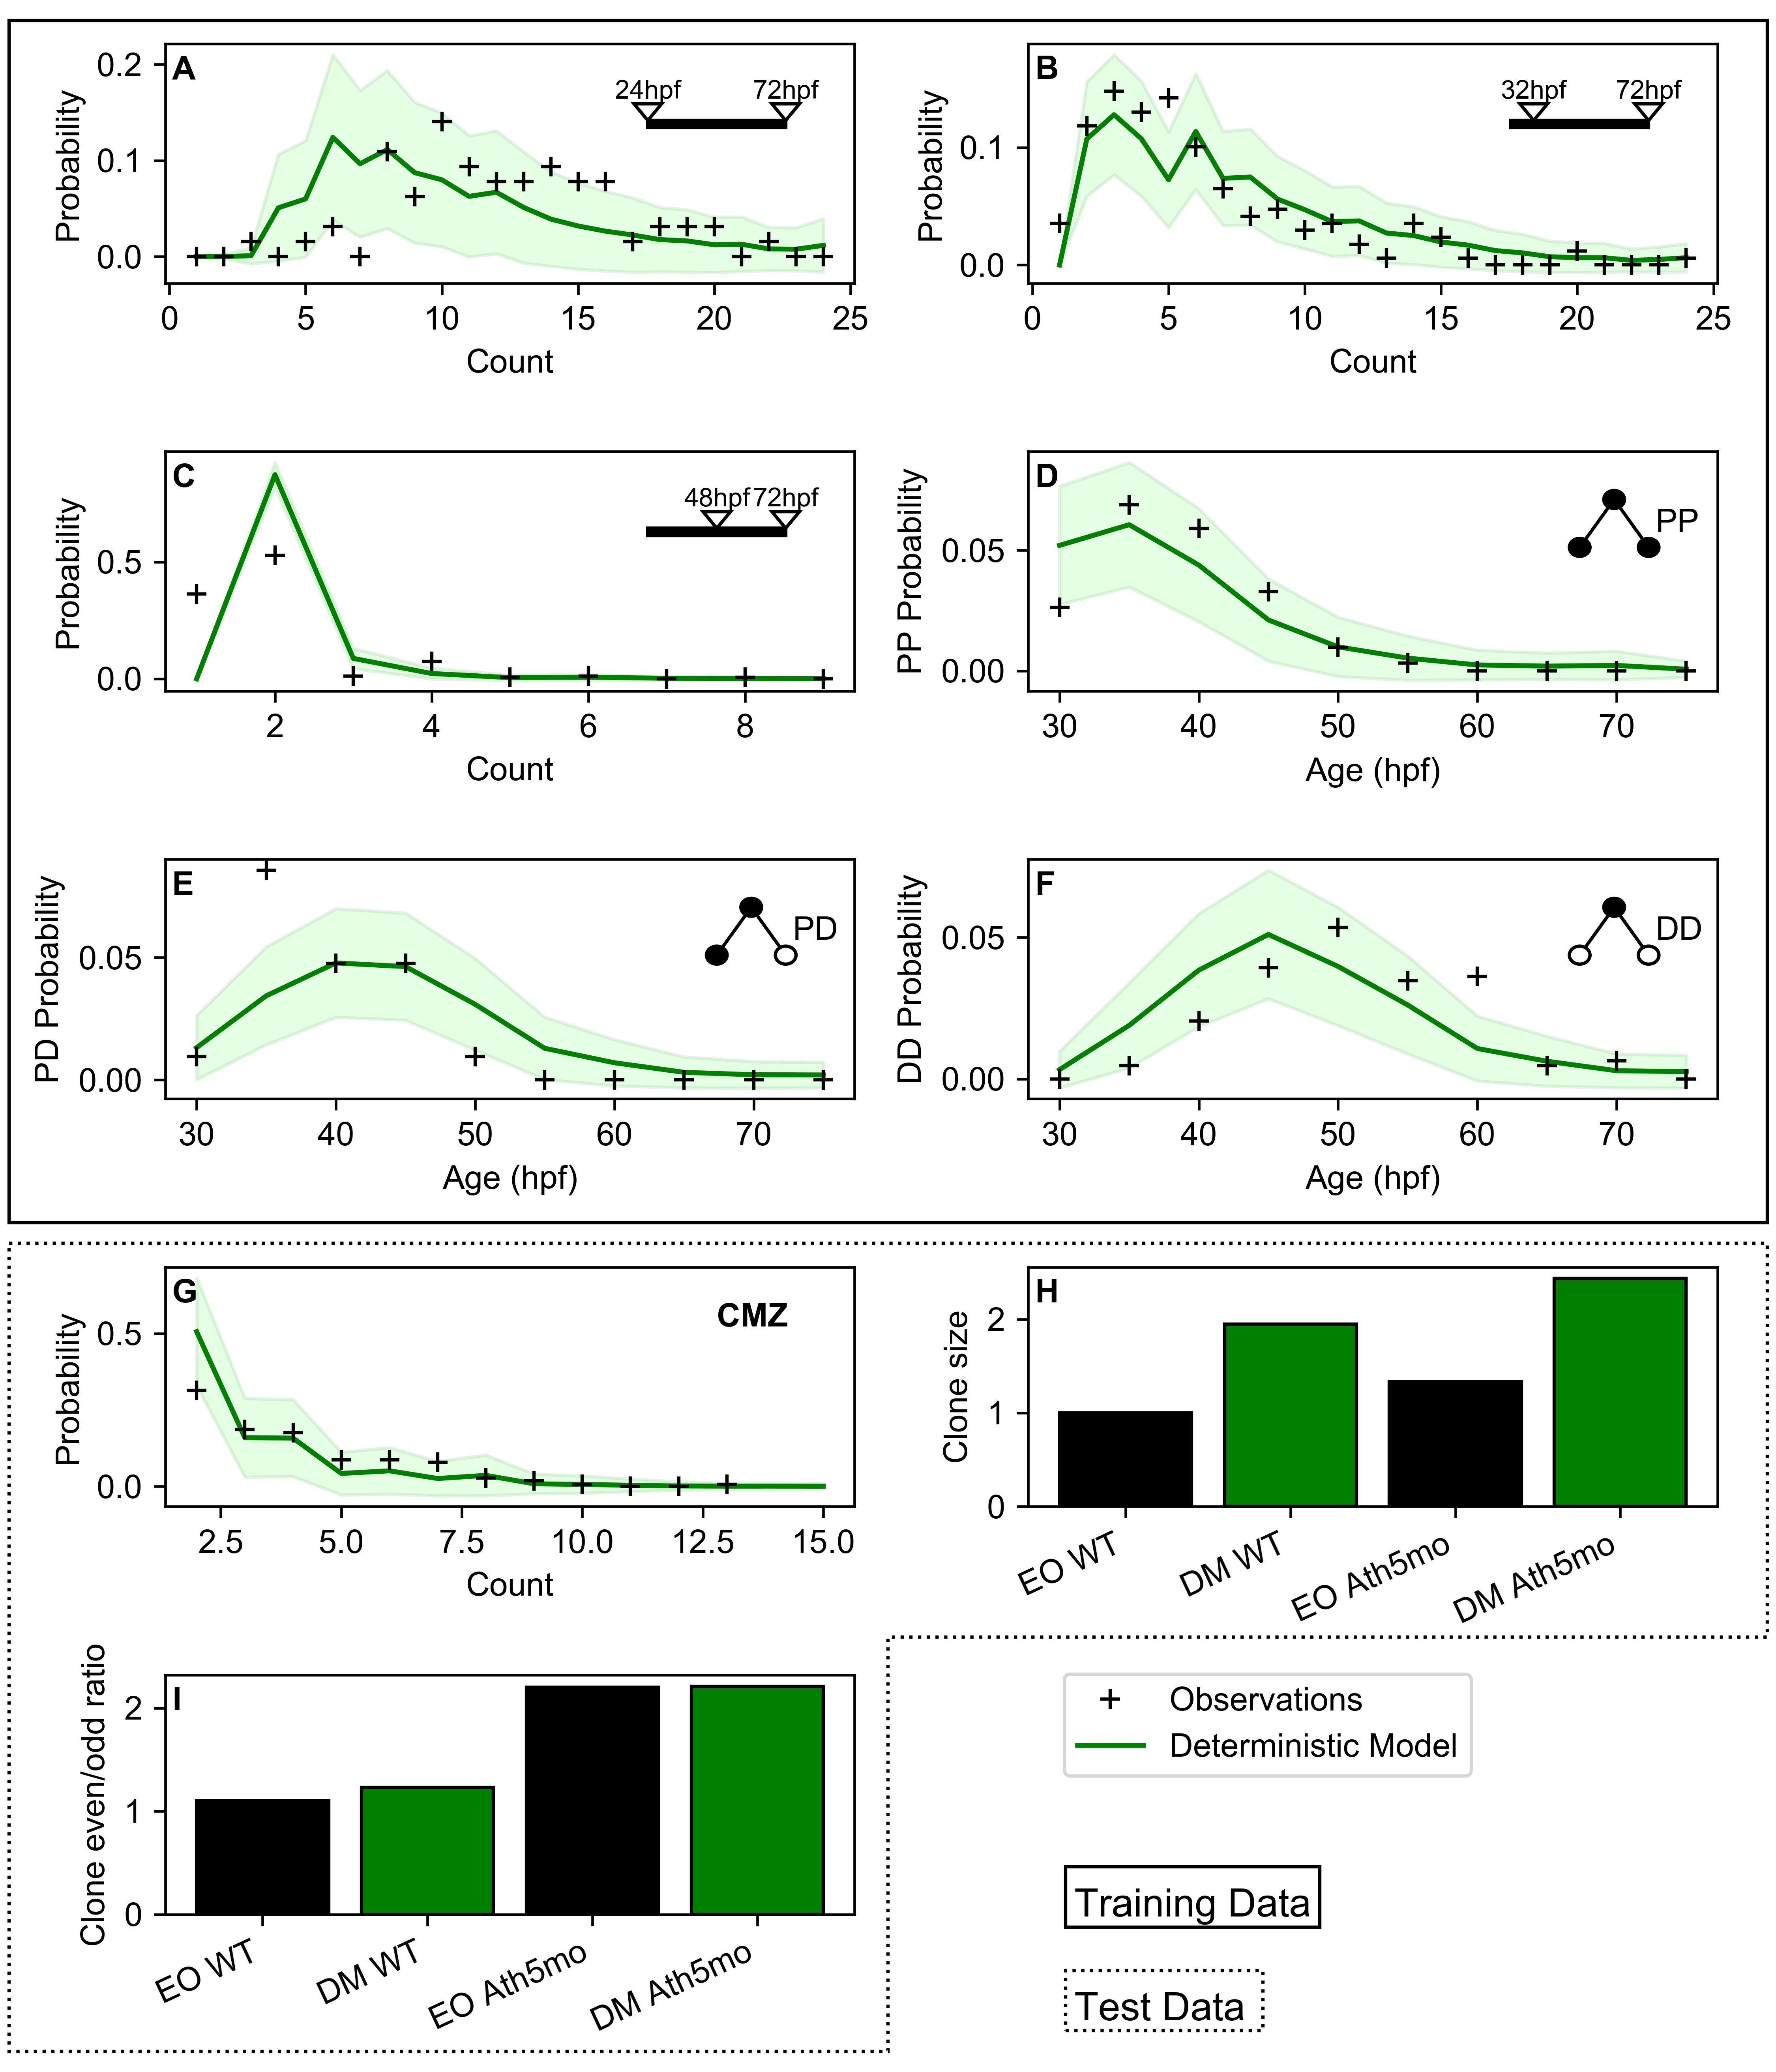
\includegraphics[width=1.\textwidth]{ssm/Fig_S3_d_fig.png}}
\paragraph{S3 Fig.}
\label{deterministicSupplement}
{\bf SPSA-optimised deterministic mitotic mode model output.} As Fig \ref{SDFig}; deterministic model output displayed by itself.
\end{figure}

\begin{figure}[h]
\makebox[\textwidth][c]{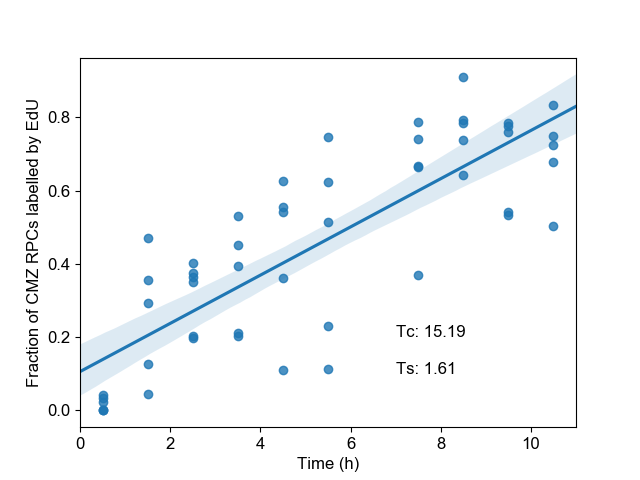
\includegraphics[width=1.\textwidth]{ssm/Fig_S4_cumulative_edu.png}}
\paragraph{S4 Fig.}
\label{cumulativeSupplement}
{\bf Cumulative EdU Labelling of 3dpf CMZ RPCs} Fraction of PCNA-labelled CMZ RPCs which bear EdU label over time, as determined by histochemical labelling of central coronal cryosections of 3dpf zebrafish retinas. Dots represent results from individual retinas. Line is the ordinary least squares fit $\pm$ 95\% CI. Cell cycle length (Tc) and S-phase length (Ts) are estimated from this fit following the method of Nowakowski et al.\cite{Nowakowski1989}
\end{figure}
\chapter{Supplementary materials for \autoref{chap:CMZ}}
\section{Materials and methods}
\subsection{Zebrafish husbandry}
Zebrafish husbandry was performed as described in \autoref{ssec:husbandry}.
\subsection{PCNA Immunohistochemistry}
Anti-PCNA immunohistochemistry was performed as described in \autoref{ssec:PCNA}.
\subsection{Thymidine analogue histochemistry}
\label{ssec:CMZEdU}
Both cumulative thymidine analogue histochemistry presented in \autoref{ssec:CMZcumedu}, as well as the pulse-chase histochemistry used for the study of neural fate in \autoref{sec:neuralfate} were performed by the methods described in \autoref{ssec:SMMEcumedu} and \autoref{ssec:SMMEwholeretina}, respectively, except that the data from the whole retinal labelling experiment derives from 14\si{micro}{metre} transverse and coronal cryosections (n=3-6 animals per axis, per age). 

\subsection{Lineage tracing immunohistochemistry}
\label{ssec:CMZlintrace}
Embryos from wild-type AB crosses (staining groups 2 and 3) and \textit{Tg(Isl2b:GFP)} crosses (staining group 1). The \textit{Tg(Isl2b:GFP)} line was the kind gift of the late Dr. Chi-Bin Chien. Embryos were collected and reared as described in \autoref{ssec:husbandry}. Embryos were divided into three groups, to be pulsed with EdU at 3, 23, and 90 dpf and sacrificed after a 7 day chase period. In 3 and 23dpf larvae, animals were pulsed by allowing them to swim freely in a 10mM EdU solution for 2 hours. In 90dpf animals, 10\si{micro}{liters} of 10mM EdU was injected intraperitoneally. After 7 days, animals were sacrificed and coronal cryosections were obtained as described in \autoref{ssec:PCNA}. These cryosections were divided into staining groups according to their genetic origin, as mentioned above.

Cryosections from all staining groups were allowed to dry briefly at room temperature (RT), before rehydration in PBS for 30 minutes at RT.  Subsequently, sections were blocked in 0.2\% Triton X-100 + 2\% goat serum in PBS for 30 minutes at RT. Primary antibody incubations were as follows for each numbered staining group:

\begin{enumerate}
    \item Covance rabbit anti-Pax6 primary antibody diluted 1:200 in blocking solution incubated at 4\degree C overnight.
    \item Chemicon mouse anti-GS primary antibody diluted 1:500 in blocking solution at 4\degree C overnight.
    \item ZIRC mouse anti-Zpr1 primary antibody diluted 1:400 in blocking solution at 4\degree C overnight.
\end{enumerate}

After these overnight incubations, primary antibodies were removed and all sections were rinsed five times in PDT (PBS + 1\% DMSO + 0.1\% Tween-20). Secondary antibody incubations were as follows for each numbered staining group:

\begin{enumerate}
    \item Goat anti-rabbit Cy3-conjugated 2º antibody diluted 1:100 in blocking solution at 37°C for 2 hr.
    \item Goat anti-mouse Cy2-conjugated 2º antibody diluted 1:100 in blocking solution at 37°C for 2 hr.
    \item Goat anti-mouse Cy2-conjugated 2º antibody diluted 1:100 in blocking solution at 37°C for 2 hr.
\end{enumerate}

Staining group 2 was subsequently incubated with Santa Cruz rabbit anti-PKC$\beta$ 1º antibody diluted 1:100 in blocking solution at 4°C overnight. The next day, this second primary antibody was removed, and the group sections were rinsed in PDT as above. A further goat anti-mouse Cy2-conjugated 2º antibody diluted 1:100 in blocking sol’n was applied at 37°C for 2 hr.

After each staining group's final secondary antibody was removed, slides were rinsed 3x in PDT, then stained for EdU with an Alexa 647 azide. After another three PDT rinses, 100 ug/mL Hoechst 33258 was applied for 15 minutes at RT. Five PDT rinses, after which all slides were mounted, slipped, and sealed.

\subsection{4C4 immunohistochemistry}
\label{ssec:CMZ4C4histo}
The 4C4 antibody was a generous gift of Dr. Pamela Raymond. It has been empirically determined to mark microglia \cite{Becker2001}. It was used according to the methods described above with a Cy2 secondary antibody.

\subsection{Confocal micrograph acquisition and processing}
All confocal micrographs presented in \autoref{chap:CMZ} were acquired on a Leica TCS SP5 II microscope, operated using the LAS AF microscopy software (Leica). Data was assessed by using Bitplane Imaris software (v.). Specifically, the Imaris watershed segmentation algorithm was applied to the nuclear counterstain channel to segment cellular nuclei. Colocalisation of particular markers (ie. PCNA, EdU, or lineage markers) was assessed by thresholding signal from these channels with the segmented nuclear volumes to produce a subpopulation of colabelled nuclei. The segmented Imaris scenes and the associated settings are available in the thesis \hyperref[archive]{HDD archive}.

\subsection{Retinal measurements}
\label{ssec:CMZretmeas}
The developmental morphology study presented in \autoref{morphology} was conducted by using the LAS AF software measurement tools on transmitted light data collected in the process of conducting the confocal survey presented in \autoref{CMZoverall}. Each measurement point is, therefore, likewise the average of the value three central coronal cryosections. Retinal thickness was the linear thickness of the entire cellular retina and its plexiform layers at the center of the section, and the layer thicknesses reflect segments along this line, with the addition of RPE thickness. RPE length was measured in approximating segments from the dorsal to the ventral extrema. Lens diameter was measured in any sections which retained the lens; this was rare at older ages, when the lens sections tend to separate readily as soon as the cryosection is rehydrated. Optic nerve diameter was measured at its thickest point.

\subsection{Estimation of overall CMZ population and retinal volume}
\label{ssec:CMZpopvolest}
The overall CMZ population estimates were derived by the calculations presented in \autoref{sec:lenspopest}. The volume of the cellular retina was crudely estimated by subtracting the volume of two spheres. The circumference of the outer sphere is given by the RPE length plus the diameter of the lens. The radius of the inner sphere is the half total thickness of the cellular retina subtracted from radius of the outer sphere\footnote{Halving serves as crude compensation for the lack of cellular retina on the lens' part of the sphere, as well as the thinning of the cellular retina toward the periphery}. The difference in volume between the two spheres is calculated; four-fifths this value is taken as the volume estimate in order to partially compensate for the flattening of the eye at older ages.

\subsection{Monte Carlo estimation of CMZ population and retinal volume rates of change}
\label{ssec:MCrates}
In order to estimate the mean daily rate of change of the CMZ population and retinal volume estimates, we performed to Monte Carlo difference operations between samples drawn from the estimated LogNormal distributions at subsequent timepoints. This allows us to empirically estimate the uncertainty on these rates, as the difference between two T-distributions is not, itself, T-distributed.


\subsection{Evidence estimation by Empirical Bayes linear regression}
\label{ssec:CMZEmpBayes}
Evidence comparisons presented without estimated standard deviations ($\sigma$) of significance are produced by the \hyperref[ssec:EmpiricalBayes]{Empirical Bayes} method of linear regression, as presented in Bishop's standard machine learning textbook \cite{Bishop2006}. Calculations were performed using the Julia package \path{BayesianLinearRegression.jl}, which implements Bishop's algorithm in a high performance manner. 


% \autoref{EBtable} summarizes the \autoref{chap:CMZ} tables and figures which use this technique, along with links to model documentation and the code used to produce the table orfigure.

% \begin{table}[!ht]
%     \caption{Empirical Bayes estimates: models and code}
%     \begin{tabular}{|l|l|l|l|l|l|l|} 
%         \hline
%         {\bf Table/Figure} & {\bf Model} & {\bf Code} \\ \hline \hline

%     \end{tabular}
%     \label{EBtable}
% \end{table}

\subsection{Evidence estimation by Galilean Monte Carlo nested sampling}
\label{ssec:GMCev}

Evidence comparisons presented with estimated standard deviations ($\sigma$) of significance are produced by converging ensembles of \hyperref[GMC]{Galilean Monte Carlo} sample chains, which collectively constitute a sample from the posterior in rigorous detailed balance \cite{Skilling2019}. The \hyperref{BayesEpistemology}[Bayesian evidence], or marginal probability of the model over the posterior sample is calculated by the \hyperref{Nested}[nested sampling algorithm] \cite{Skilling2006}. Calculations were performed by the use of the Julia packages \path{GMC_NS.jl} and \path{CMZNicheSims.jl}, written for this thesis and presented in \autoref{chap:GMC} and \autoref{chap:CNS}, respectively. Maximum a posteriori outputs are calculated from the most likely model parameterisation sampled during this process.

% \autoref{GMCtable} summarizes the \autoref{chap:CMZ} figures which use these techniques, along with links to model documentation and the code used to produce the figures.

% \begin{table}[!ht]
%     \caption{Galilean Monte Carlo estimates: models and code}
%     \begin{tabular}{|l|l|l|l|l|l|l|} 
%         \hline
%         {\bf Table/Figure} & {\bf Model} & {\bf Code} \\ \hline \hline
%         \autoref{PZRtable} & \hyperref[NormalModels]{Normal \& LogNormal} & \autoref{ssec:a10nvln} \\ \hline
%     \end{tabular}
%     \label{GMCtable}
% \end{table}

\subsection{Estimation of posterior distributions of phase model parameters}
\label{ssec:GMCkde}
Posterior distributions presented in \autoref{phasemarginals} and \autoref{dvmarginals} were produced by Kernel Density Estimation (KDE) \cite[p. 122]{Bishop2006}. The KDE algorithm used was the implementation available in the Julia Robotics library \path{KernelDensityEstimate.jl}, described by Sudderth et al. \cite{Sudderth2010}. Briefly, this uses multiscale nonmparametric Gibbs sampling of supplied weighted ``point clouds'' to generate the kernel density estimate. Chains from \path{GMC_NS.jl} were used in this context by weighting the points in parameter space by their estimated evidence. It is important to note that, for this thesis, \path{GMC_NS.jl} was configured to prioritise the accuracy of evidence estimates over these posterior estimates; as a consequence, samples from around the maximum a posteriori have little weight in the KDE estimates presented herein \cite{Higson2018}. Alternatives to this scheme are possible; one such algorithm is described by Higson et al. \cite{Higson2019}

\section{Supplementary Figures}

\begin{figure}[!h]
    \makebox[\textwidth][c]{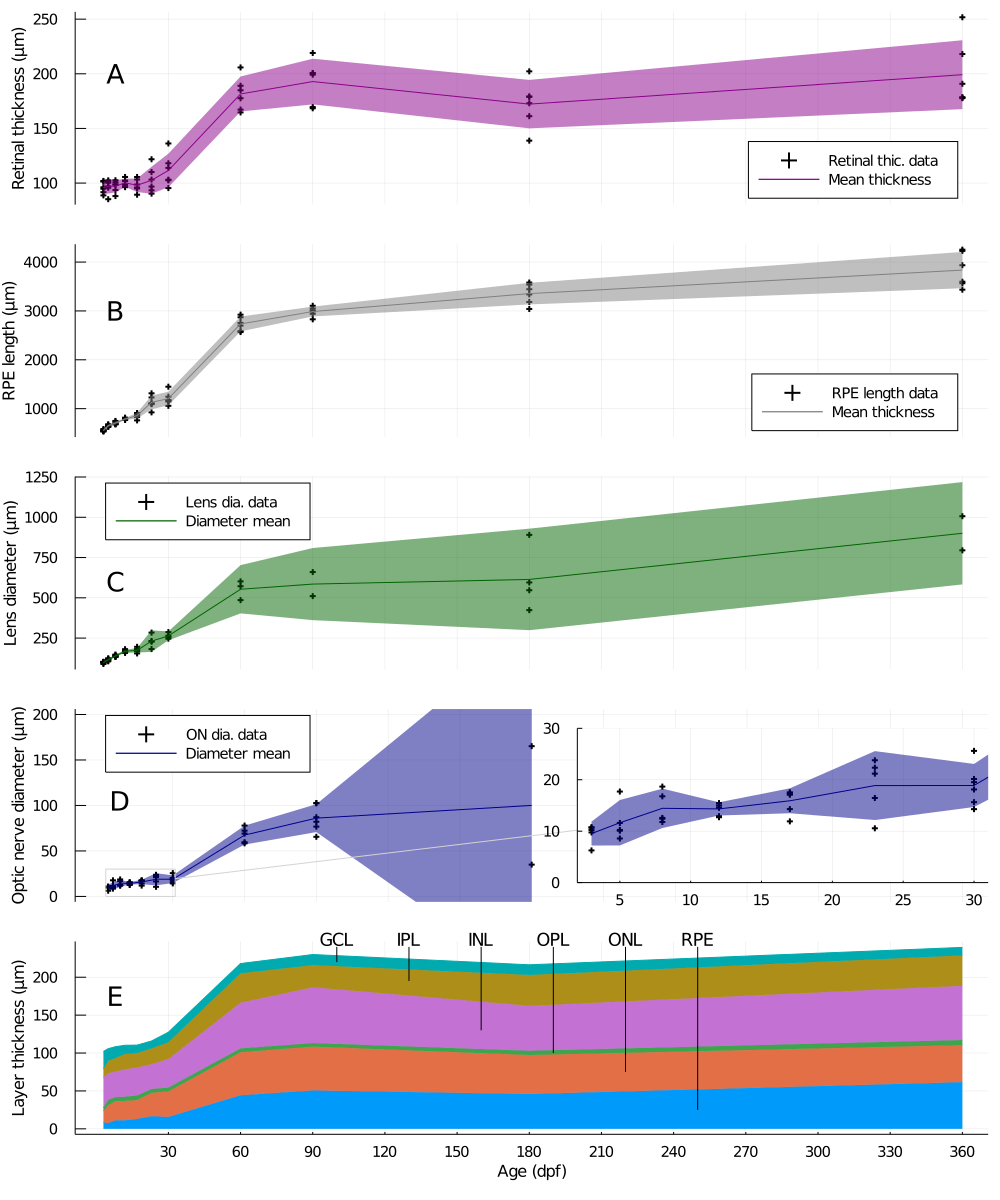
\includegraphics[width=1.2\textwidth]{cmz/morphology.png}}    
    \caption{{\bf Developmental progression of naso-temporal population asymmetry in the CMZ.}}
    \label{morphology}
\end{figure}

\begin{figure}[!h]
    \makebox[\textwidth][c]{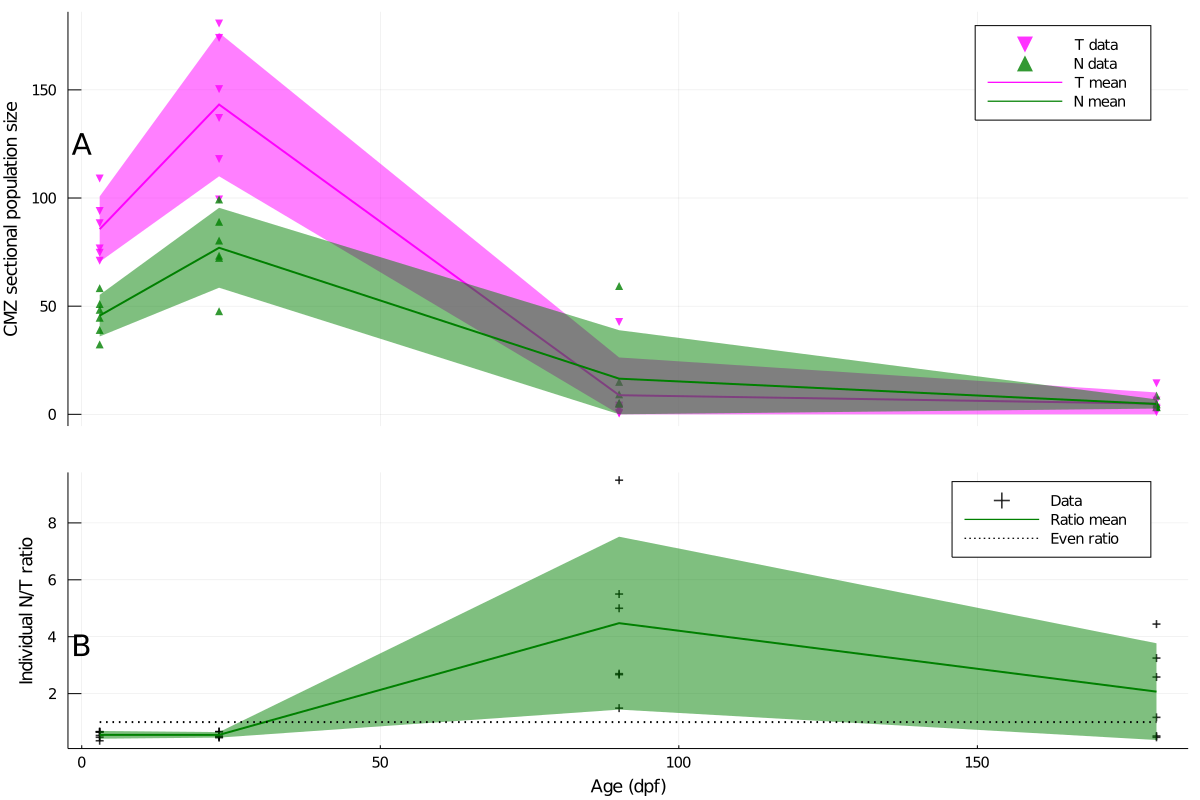
\includegraphics[width=1.2\textwidth]{cmz/NTontology.png}}    
    \caption{{\bf Developmental progression of naso-temporal population asymmetry in the CMZ.}}
    Marginal posterior distribution of mean nasal (N) and temporal (T) population size in 14$\mu$m transverse cryosections (panel A) or intra-individual N/T count asymmetry ratio (panel B), $\pm 95\%$ credible interval, n=6 animals per age. Data points represent mean counts from three central sections of an experimental animal's eye. 
    \label{NTontology}
\end{figure}


\begin{figure}[!h]
    \makebox[\textwidth][c]{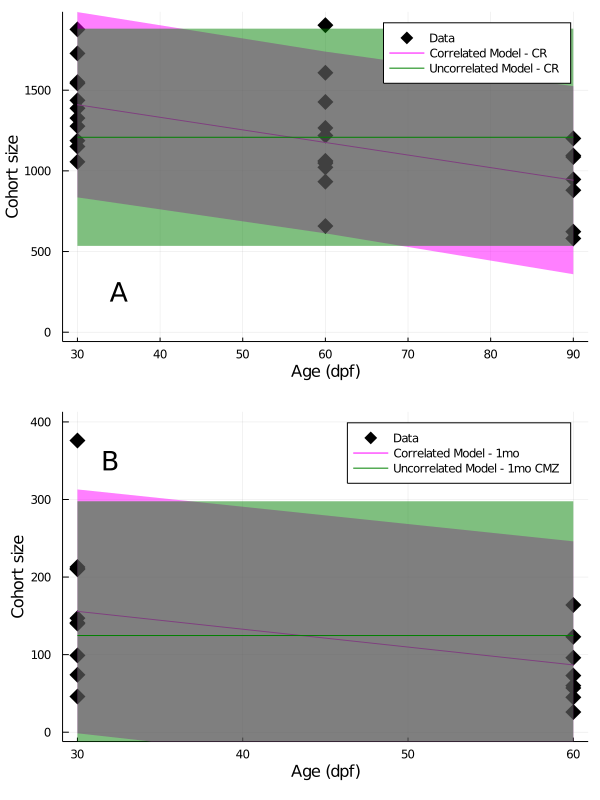
\includegraphics[width=.7\textwidth]{cmz/a27linreg.png}}    
    \caption{{\bf Linear regressions of temporally correlated and uncorrelated models of central retinal and 30dpf CMZ-contributed cohorts}}
    \label{a27linreg}
\end{figure}


\begin{figure}[!h]
    \makebox[\textwidth][c]{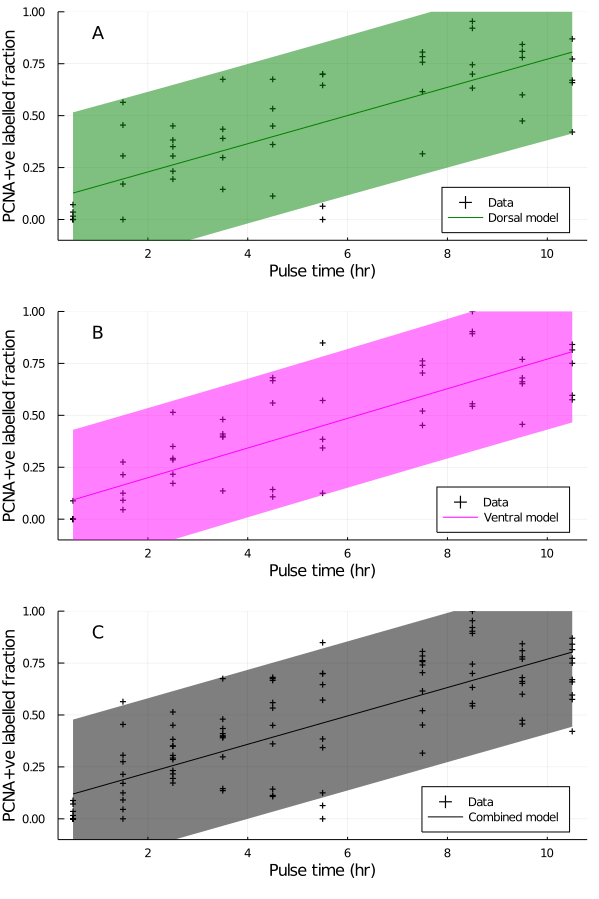
\includegraphics[width=.7\textwidth]{cmz/3ddvlinreg.png}}    
    \caption{{\bf Linear regressions performed on cumulative labelling data from dorsal, ventral, and combined CMZ sectional populations}}
    \label{cumEdUlinreg}
\end{figure}

\begin{figure}[!h]
    \makebox[\textwidth][c]{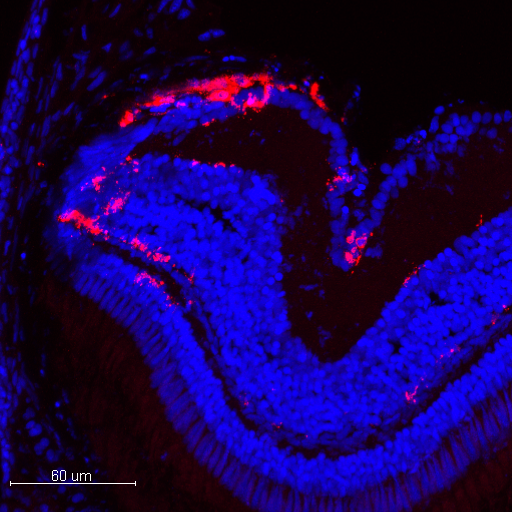
\includegraphics[width=.6\textwidth]{cmz/4C4 distribution.png}}    
    \caption{{\bf 4C4+ microglia are associated with the CMZ}}
    Representative maximum intensity projection from confocal micrographs of 14\si{\micro\metre} coronal cryosections through 90dpf zebrafish eyes.
    
    Blue: Hoechst 33258 nuclear counterstain. Red: Microglia labelled with 4C4 antibody. Note extensive presence of 4C4+ microglia around the peripheral CMZ.
    \label{4C4micrograph}
\end{figure}

\FloatBarrier

\section{Evidence calculations for models of layer and lineage contribution}
\FloatBarrier

\begin{table}[!ht]
    \caption{Evidence for Normal vs. Log-Normal models of layer and lineage contribution}
    \begin{tabular}{|l|l|l|l|l|l|l|} 
        \hline
        {\bf Layer} & {\bf Marker} & {\bf Cell type} & {\bf $\mathcal{N}$ logZ} & {\bf Log-$\mathcal{N}$ logZ} & {\bf logZR} & {\bf $\sigma$ sign.}\\ \hline \hline
        GCL & Cohort & All GCL cells & -92.81 ± 0.56 & {\bf-63.93 ± 0.19} & 28.88 ± 0.6 & 48.5\\ \hline \hline
        GCL & Isl2b & RGC & -56.3 ± 0.76 & {\bf -46.91 ± 0.35} & 9.38 ± 0.84 & 11.2\\ \hline
        GCL & Pax6 & Displaced am. & -110.7 ± 1.2 & {\bf -35.39 ± 0.34} & 75.3 ± 1.2 & 62.1\\ \hline
        GCL & Isl2b/Pax6 & RGC subtype & -16.38 ± 0.18 & {\bf -3.25 ± 0.6} & 13.13 ± 0.63 & 20.9\\ \hline \hline
        INL & Cohort & All INL cells & {\bf -84.56 ± 0.91} & -286.89 ± 0.68 & -202.3 ± 1.1 & 178.3\\ \hline \hline
        INL & Pax6 & Amacrine cell & {\bf -13.99 ± 0.24} & -18.5 ± 0.25 & -4.52 ± 0.35 & 12.9\\ \hline
        INL & PKC$\beta$ & Bipolar cell & -13.66 ± 0.16 & {\bf 8.68 ± 0.44} & 22.34 ± 0.47 & 47.7\\ \hline
        INL & GS & M\"{u}ller glia & -12.36 ± 0.23 & {\bf 14.18 ± 0.48} & 26.54 ± 0.53 & 50.3\\ \hline
        INL & HM & Horizontal cell & -16.44 ± 0.27 & {\bf 9.15 ± 0.37} & 25.59 ± 0.46 & 55.6\\ \hline \hline
        ONL & Cohort & All ONL cells & {\bf -128.68 ± 1.0} & -171.66 ± 0.63 & -43.0 ± 1.2 & 36.5\\ \hline \hline
        ONL & Zpr1 & Double cones & {\bf -42.25 ± 0.72} & -54.25 ± 0.37 & -11.99 ± 0.81 & 14.9\\ \hline
    \end{tabular}
   
    \begin{flushleft}logZ: logarithm of p(D), the marginal likelihood of the data, or model evidence.  Largest evidence values bolded. logZR: evidence ratio; positive values in favour of Log-$\mathcal{N}$ model.
    \end{flushleft}
    \label{lineage_nlnev}
\end{table}

\begin{table}[!ht]
    \caption{Evidence for combined vs. split models of layer and lineage contribution across the dorso-ventral axis}
    \begin{tabular}{|l|l|l|l|l|l|l|} 
        \hline
        {\bf Layer} & {\bf Marker} & {\bf Cell type} & {\bf Combined D-V logZ} & {\bf Split D-V logZ} & {\bf logZR} & {\bf $\sigma$ sign.}\\ \hline \hline
        GCL & Cohort & All GCL cells & {\bf -53.473 ± 0.055} & -184.34 ± 0.13 & 130.86 ± 0.14 & 911.5\\ \hline \hline
        GCL & Isl2b & RGC & {\bf -54.58 ± 0.9} & -67.72 ± 0.94 & 13.1 ± 1.3 & 10.1\\ \hline
        GCL & Pax6 & Displaced am. & {\bf -31.09 ± 0.12} & -46.41 ± 0.3 & 15.32 ± 0.33 & 46.9\\ \hline
        GCL & Isl2b/Pax6 & RGC subtype & {\bf -43.76 ± 0.76} & -109.0 ± 1.3 & 65.3 ± 1.5 & 43.3\\ \hline \hline
        INL & Cohort & All INL cells & {\bf -131.4 ± 1.4} & -184.4 ± 1.6 & 52.9 ± 2.1 & 25.0\\ \hline \hline
        INL & Pax6 & Amacrine cell & {\bf -15.8 ± 0.024} & -52.42 ± 0.69 & 36.62 ± 0.69 & 53.3\\ \hline
        INL & PKC$\beta$ & Bipolar cell & {\bf -3.86 ± 0.2} & -19.81 ± 0.23 & 15.96 ± 0.31 & 51.9\\ \hline
        INL & GS & M\"{u}ller glia & {\bf 15.78 ± 0.25} & 28.03 ± 0.41 & -12.24 ± 0.48 & -25.6\\ \hline
        INL & HM & Horizontal cell & {\bf 10.79 ± 0.41} & -3.65 ± 0.19 & 14.45 ± 0.45 & 32.2\\ \hline \hline
        ONL & Cohort & All ONL cells & {\bf -79.87 ± 0.97} & -158.2 ± 1.3 & 78.3 ± 1.6 & 48.5\\ \hline \hline
        ONL & Zpr1 & Double cones & {\bf -54.66 ± 0.92} & -64.27 ± 0.87 & 9.6 ± 1.3 & 7.6\\ \hline
    \end{tabular}
\begin{flushleft}logZ: logarithm of p(D), the marginal likelihood of the data, or model evidence.  Largest evidence values bolded. logZR: evidence ratio; positive values in favour of combined model.
\end{flushleft}
\label{lineage_dvev}
\end{table}

\section{Likelihood ratio calculations for Normal and Log-Normal models of layer and lineage contribution}

\begin{table}[!ht]
    \begin{tabular}{|l|l|l|l|l|l|l|} 
        \hline
        {\bf Layer} & {\bf Marker} & {\bf Cell type} & {\bf $\mathcal{N}$ MLE} & {\bf Log-$\mathcal{N}$ MLE} & {\bf lhR}\\ \hline \hline
        GCL & Cohort & All GCL cells & 54.194 & {\bf 55.835} & 1.642\\ \hline
        GCL & Isl2b & RGC & 14.439 & {\bf 19.106} & 4.667\\ \hline
        GCL & Pax6 & Displaced am. &  8.287 & {\bf 11.158} & 2.871\\ \hline
        GCL & Isl2b/Pax6 & RGC subtype & 20.292 & {\bf 28.139} & 7.847\\ \hline
        INL & Cohort & All INL cells & 44.942 & {\bf 45.179} & 0.237\\ \hline
        INL & Pax6 & Amacrine cell & {\bf 23.808} & 23.178 & -0.63\\ \hline
        INL & PKC$\beta$ & Bipolar cell & {\bf 27.243} & 26.119 & -1.124\\ \hline
        INL & GS & M\"{u}ller glia & 30.847 & {\bf 31.818} & 0.97\\ \hline
        INL & HM & Horizontal cell & 27.65 & {\bf 29.431} & 1.78\\ \hline
        ONL & Cohort & All ONL cells & 41.488 & {\bf 43.195} & 1.706\\ \hline
        ONL & Zpr1 & Double cones & 13.256 & {\bf 18.483} & 5.227\\ \hline
    \end{tabular}
   
    \begin{flushleft}logZ: logarithm of p(D), the marginal likelihood of the data, or model evidence.  Largest evidence values bolded. logZR: evidence ratio; positive values in favour of stable model.
    \end{flushleft}
    \label{lineage_lhratio}
\end{table}



\chapter{Supplementary material for \autoref{chap:rys}}
\section{Materials and methods}
\subsection{Zebrafish husbandry}
Zebrafish husbandry was performed as described in \autoref{ssec:husbandry}.

\subsection{Generation of transgenic vsx2:eGFP \textit{rys} line}
\autoref{progenitoridentity} makes use of coronal cryosections of \textit{Tg(vsx2:eGFP)} \textit{rys} animals. Transgenesis was performed using reagents from the Tol2kit \cite{Kwan2007}, which uses the Invitrogen Gateway plasmid construction system to assemble three-part constructs from donor plasmids. 

\subsection{Morpholino injections}
 
\subsection{Morphological photography}

\subsection{PCNA and EdU proliferative histochemistry}

\subsection{Progenitor identity marker immunohistochemistry}

\subsection{BrdU pulse-chase assays}

\subsection{Caspase-3 immunohistochemistry}

\subsection{Pax6 immunohistochemistry}

\subsection{In situ hybridization}

\subsection{Electron microscopy}

\subsection{Analysis of \textit{rys} nuclear parameters by Galilean Monte Carlo Nested Sampling}

\subsection{RT-PCR analysis of \textit{rys} npat expression}

\subsection{\textit{rys} MNase digestions and NGS}

\subsection{Nucleosome position calling}
The nucleosome position calling pipeline used in \autoref{chap:rys} was automated using the Java machine learning framework KNIME \cite{Dietz2016} workspace incorporating KNIME4NGS nodes \cite{Hastreiter2017}. The pipeline is depicted in figureautoref. Node settings are largely default and are available in the \path{knime_workspace} \hyperref[sec:archive]{thesis archive}.

Briefly, FastQC (v0.11.8) \cite{Andrews2018} was used to characterise the quality of the fastq sequence files describing the nucleosome-protected fragment pool from the MNase digestions described above. No sequence from any of the two duplicates of the two pools was rejected due to low quality. Sequences were found to be of uniformly high quality, with low adapter content. These results are available in the \path{fastqc} \hyperref[sec:archive]{thesis git archive}. TrimGalore (v0.5.0) \cite{Andrews2018a} was used to remove trailing adapter bases, using Adapter sequence: 'AGATCGGAAGAGC' (Illumina TruSeq, Sanger iPCR). The trim reports are available in the \hyperref[sec:archive]{thesis git archive}.  Bowtie 2 \cite{Langmead2012} with default settings was used to map reads to the zebrafish genome (GRCz11). Nucleosome positions were called from the resulting sequence alignment map (SAM) files by using DANPOS2 (v2.2.2) \cite{Chen2013}. As DANPOS2 is no longer supported, and the code contained errors preventing execution, a fixed version of this code has been uploaded to \path{https://github.com/mmattocks/DANPOS2fix} and filed in the \hyperref[sec:archive]{thesis HDD archive}, along with the called output positions.

The DANPOS nodes of the KNIME workflow are python nodes which execute DANPOS2 itself, as well as the nucleosome position analyses described below. 

\subsection{Analyses of \textit{rys} nucleosome position disposition}
\autoref{nucgendist} was produced from the DANPOS2-called positions for the pooled \textit{rys} sibling and mutant MNase-protected fragment datasets. For each numbered \textit{D. rerio} chromosomal scaffold (1-25), as well as for scaffolds not assigned to any chromsome (NC), the number of sibling positions was divided by the total length of the scaffold. These values were compared to the naively expected number of positions per scaffold, determined by dividing the total number of positions per kilobase of genomic material, then multiplying the particular scaffold length. The per-chromosome relative number of positions, as well as fold-differences from the naive expected value, are displayed in pie chart format in Panel A. The Panel C chart displays the result of normalizing these position values by relative occupancy, as determined by DANPOS2. 

\subsubsection{Background Hidden Markov modelling of \textit{D. rerio} genomic sequence emission}
The Julia package \path{BioBackgroundModels.jl} was used to perform background Hidden Markov Model selection on samples of \textit{D. rerio} genomic material, in order to serve as a model of genomic noise for subsequent \hyperref[ICA]{Independent Component Analysis} (ICA) modelling of nucleosome positions, described below. The general strategy pursued was to first train a zoo of 3 replicates each of all HMMs with 1-6 states, emitting 0\textsuperscript{th}-2\textsuperscript{nd} order DNA kmers, on each of three broad partitions of the GRCz11 zebrafish genome, as described in \autoref{chap:BBM}, and initializing the zoo's EM chains using the default \path{autotransition_init} function, which samples from an uninformative prior on state emission vectors, but a transition matrix prior heavily favouring state autotransition. This zoo was converged to an EM step likelihood delta of \num{1e-3} on \num{2e6} bp sampled without replacement from each of these partitions, then evaluated by testing against a further \num{2e6} bp sampled as a test set. The best model triplicate for each partition, in every case the 6 state, 0th order triplicate, was selected for further refinement by EM training on a new \num{8e6} bp sampled from the appropriate partitions. After this refinement process was complete, the triplicate chains were inspected using \path{BioBackgroundModels.jl}'s reports. The convergence of the triplicate on the same region of the parameter space, and the stationarity of the chains were verified before selecting the most likely models of the refined triplicate to represent \textit{D. rerio} genomic background noise in the \path{BioMotifInference.jl} ICA models.

The code to sample GRCz11 for the initial zoo training task is available in \autoref{ssec:BBMsampleprep}, for the refinement task in \autoref{ssec:BBMrefinementprep}. EM execution code is found in \autoref{ssec:BBMsurvey} and \autoref{ssec:BBMsurveyrefinement}. Analysis code is given in \autoref{ssec:BBMsurveyanalysis} and \autoref{ssec:BBMrefinementanalysis}.

\subsection{Evidence and maximum a posteriori estimation of ICA models of \textit{rys} nucleosome position sequence emission}

\section{Supplementary figures}

\begin{sidewaysfigure}[!h]
    \makebox[\textwidth][c]{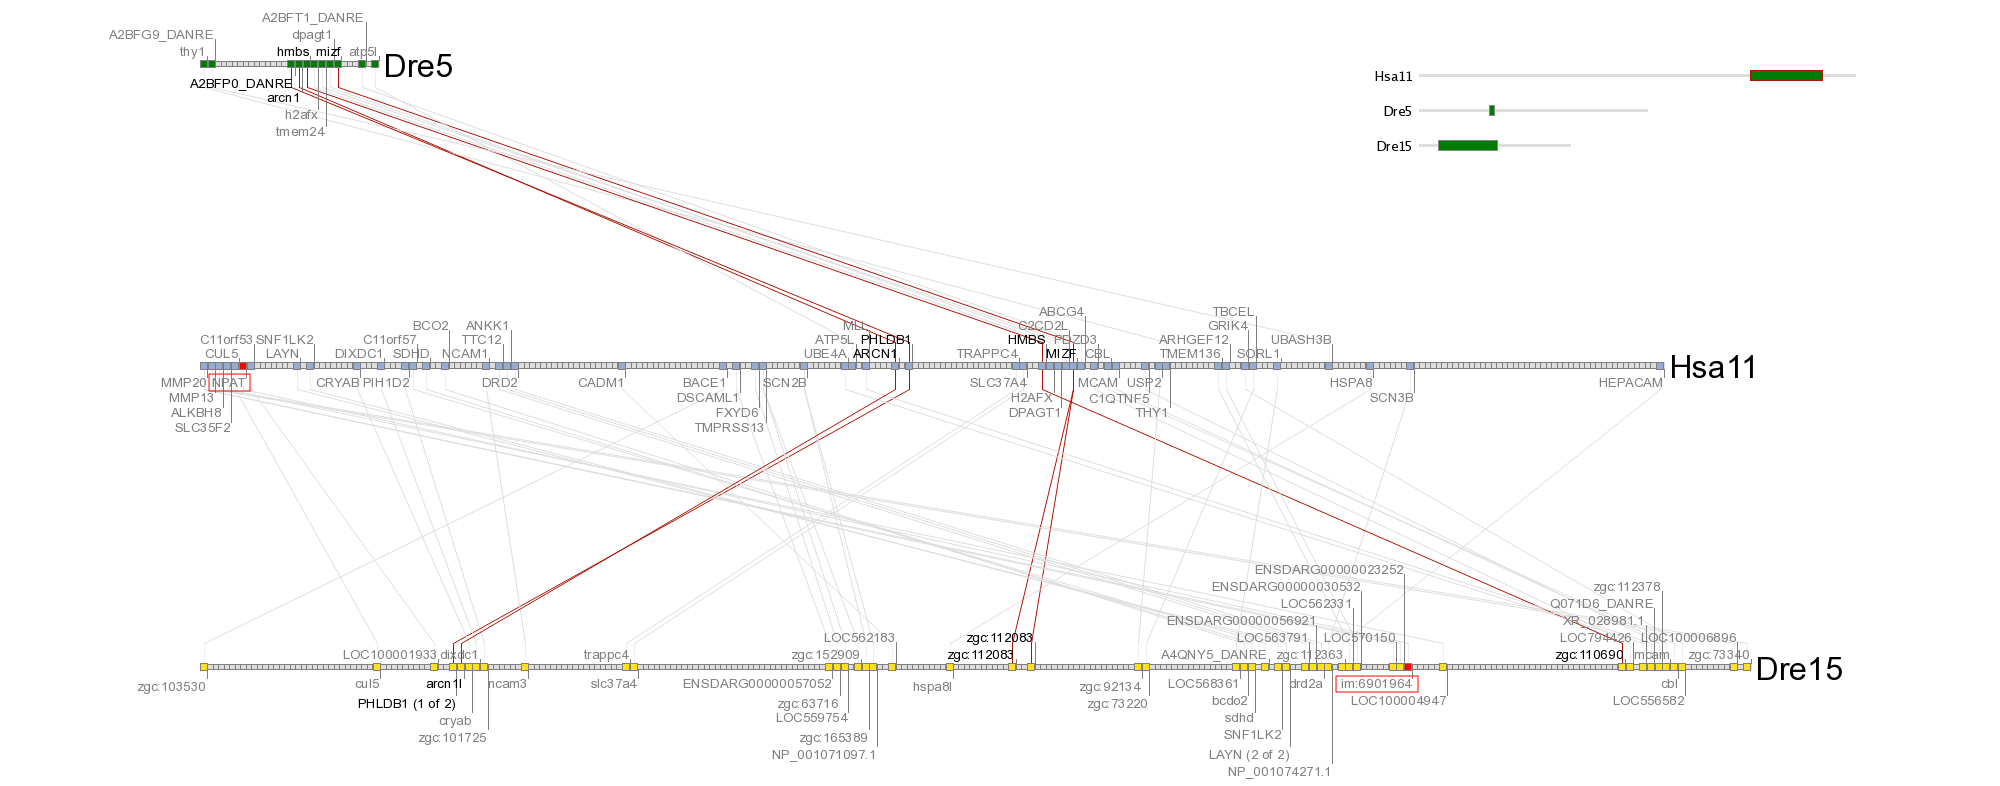
\includegraphics[width=1.2\textwidth]{rys/synteny2.png}}    
    \caption{{\bf Synteny Database output for the syntenic region containing \textit{D. rerio} npat}}
    Dre\#: \textit{Danio rerio chromosome \#}
    Hsa\#: \textit{Homo sapiens chromosome \#}

    The relative position of the displayed genomic neighbourhoods on their chromosome scaffolds is displayed inset, top right. \textit{D. rerio} npat is highlighted with a red square, visible on the right of the selected Dre15 region, annotated ``im:6901964''. \textit{H. sapiens} NPAT is highlighted similarly on the left of Hsa11. landmarks of the duplication and rearrangement event that brackets the position of npat on Dre15 are highlighted with red lines.

    On the scaffold of \textit{H. sapiens} chromosome 11, NPAT occurs upstream of the highlighted duplication cluster bracketed by ARCN1 and MIZF. Zebrafish npat is located in the midst of this rearranged, duplicated cluster, but does not appear to have been duplicated itself; at least if it was, no paralogue can be found by syntenic or similarity analysis.
    \label{synteny}
\end{sidewaysfigure}


\begin{figure}[!h]
    \makebox[\textwidth][c]{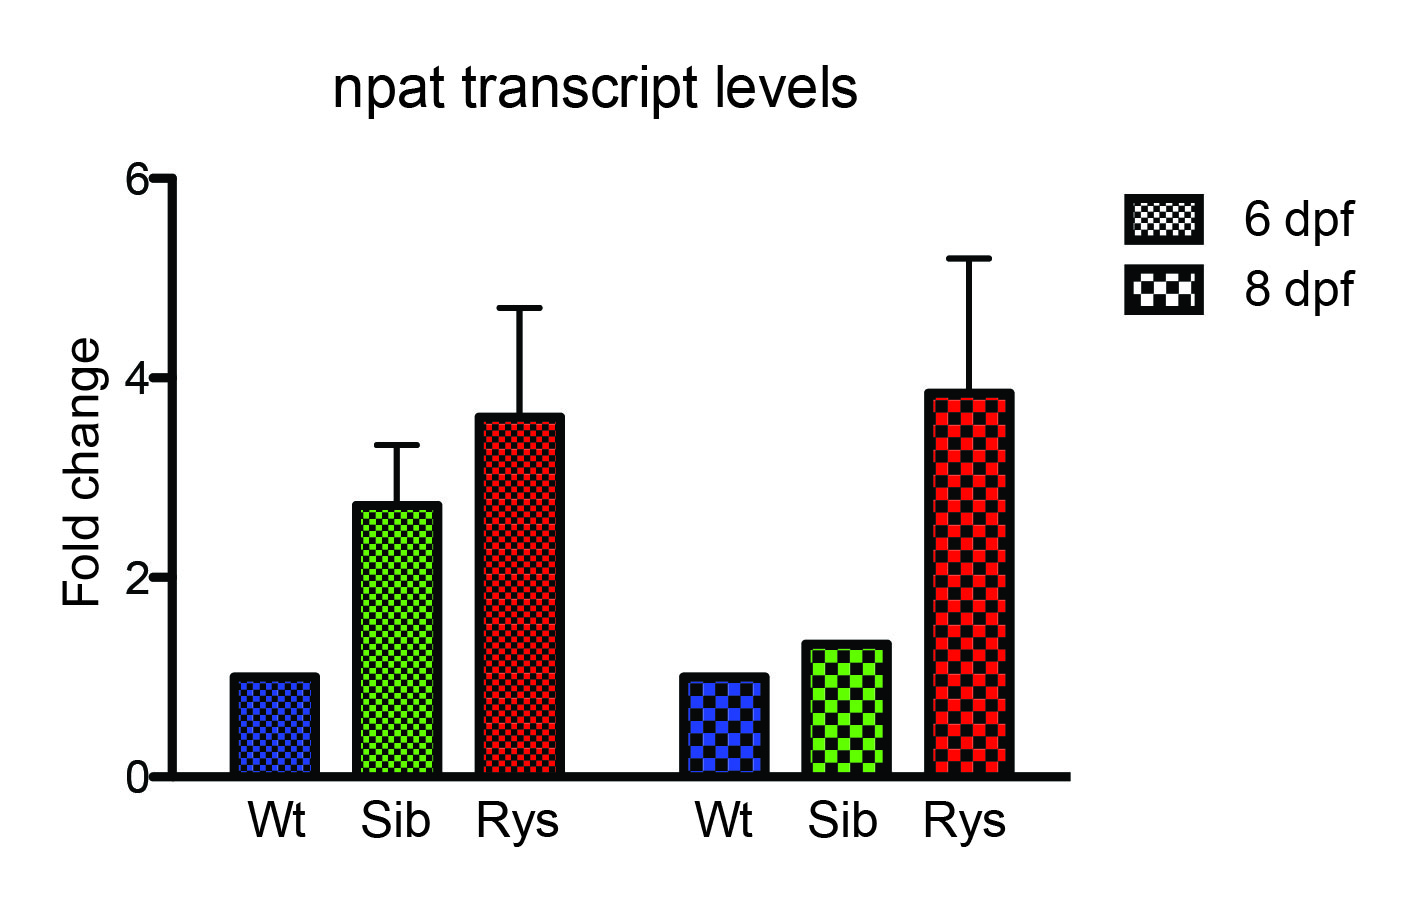
\includegraphics[width=1.\textwidth]{rys/npat transcripts.jpg}}    
    \caption{{\bf npat is overexpressed in \textit{rys}}} 
    \label{npatrtpcr}
\end{figure}

\begin{figure}[!h]
    \makebox[\textwidth][c]{\includegraphics[width=1.\textwidth]{rys/cmzfailure.png}}    
    \caption{{\bf 10dpf mutant \textit{rys} RPCs are mitotic}} MIP 14\si{\micro\metre} coronal cryosections through representative sib (left panels) and \textit{rys} eyes at 10dpf, 7 days after an 8hr BrdU pulse at 3dpf. Note that few labelled \textit{rys} cells have entered the specified retinal layers.
    \label{rysmitosis}
\end{figure}

\begin{figure}[!h]
    \makebox[\textwidth][c]{\includegraphics[width=1.\textwidth]{rys/rys_4c4.png}}    
    \caption{{\bf 4C4-positive microglia engulf \textit{rys} mutant RPCs}} 
    \label{phagocytosis}
\end{figure}


\begin{figure}[!h]
    \makebox[\textwidth][c]{\includegraphics[width=1.\textwidth]{rys/morpholinoqPCR.png}}    
    \caption{{\bf Morpholinos directed to npat result in histone transcript overexpression similar to \textit{rys}}} 
    \label{morpholinoRTPCR}
\end{figure}


\begin{figure}[!h]
    \makebox[\textwidth][c]{\includegraphics[width=.9\textwidth]{rys/chr_unique_positions.png}}    
    \caption{{\bf Novel nucleosome positions in \textit{rys} occur in similar numbers to those lost from sibs.}}
    Counts of positions found in sib but not \textit{rys} (red bars, represented as negative numbers, as these are `lost' in \textit{rys}) and those found in \textit{rys} but not sib (blue bars, `gained'). The magnitude of the difference between the counts is represented with a yellow bar.
    \label{diffposdist}
\end{figure}

\begin{figure}[!h]
    \makebox[\textwidth][c]{\includegraphics[width=.75\textwidth]{rys/bghmm.png}}    
    \caption{{\bf Test likelihoods for background HMMs trained on \textit{D. rerio} genome partitions}}
    \label{BHMMlh}
\end{figure}

\begin{figure}[!h]
    \makebox[\textwidth][c]{\includegraphics[width=.75\textwidth]{rys/combined_e_srcs.png}}    
    \caption{{\bf PWM sources detected in combined sib and rys differential sources.}}
    PWMs presented as sequence logos with letter height proportional to position informational content\/emission probability.
    
    PP: Posterior prevalence; proportion of models within the compressed maximum a posteriori ensemble which have this PWM as a signal source

    OP: Observation prevalence; mean proportion of observed position sequences this sequence is used to explain, over all posterior samples
    \label{combinedmotifs}
\end{figure}

\FloatBarrier

\section{Supplementary tables}

\begin{table}[!ht]
    \caption{Evidence for Normal vs. Log-Normal models of layer and lineage contribution}
    \begin{tabular}{|l|l|l|l|l|l|} 
        \hline
        {\bf Morpholino} & {\bf Measurement} & {\bf Separate logZ} & {\bf Combined logZ} & {\bf logZR} & {\bf $\sigma$ sign.}\\ \hline \hline
        ATG & CMZ pop. & -236.4 ± 2.3 & {\bf -198.3 ± 2.2} & -38.1 ± 3.2 & 12.1 \\ \hline
        ATG & Total sectional pop. & -412.4 ± 7.8 & {\bf -225.3 ± 4.9} & -187.1 ± 9.2 & 20.3 \\ \hline
        ATG & Sectional pop. per CMZ cell & {\bf -70.18 ± 0.86} & -78.0 ± 0.86 & 7.8 ± 1.2 & 6.4 \\ \hline
        ATG & Dorsal CMZ pop. & -169.5 ± 1.4 & {\bf -151.75 ± 0.8} & -17.8 ± 1.6 & 11.2 \\ \hline
        ATG & Ventral CMZ pop. & -223.1 ± 1.5 & {\bf -165.3 ± 1.0} & -57.8 ± 1.8 & 32.5 \\ \hline
        ATG & Nuclear volume & -290.6 ± 1.8 & {\bf -192.7 ± 1.8} & -97.9 ± 2.5 & 39.6 \\ \hline
        ATG & Nuclear sphericity & {\bf -186.13 ± 0.79} & -215.66 ± 0.57 & 29.53 ± 0.97 & 30.3 \\ \hline
        Spl & CMZ pop. & -272.6 ± 2.4 & {\bf -197.0 ± 2.6} & -75.7 ± 3.6 & 21.2 \\ \hline
        Spl & Total sectional pop. & -455.9 ± 8.3 & {\bf -205.6 ± 4.7} & -250.3 ± 9.5 & 26.3 \\ \hline
        Spl & Sectional pop. per CMZ cell & -87.04 ± 0.17 & {\bf -66.22 ± 0.29} & -20.82 ± 0.34 & 62.0 \\ \hline
        Spl & Dorsal CMZ pop. & -226.2 ± 1.7 & {\bf -171.0 ± 1.1} & -55.2 ± 2.0 & 27.7 \\ \hline
        Spl & Ventral CMZ pop. & -234.97 ± 0.81 & {\bf -222.3 ± 1.7} & -12.7 ± 1.9 & 6.8 \\ \hline
        Spl & Nuclear volume & -277.5 ± 1.6 & {\bf -223.2 ± 2.1} & -54.3 ± 2.7 & 20.4 \\ \hline
        Spl & Nuclear sphericity & -94.3 ± 1.1 & {\bf -67.71 ± 0.39} & -26.6 ± 1.1 & 23.2 \\ \hline
    \end{tabular}
   
    \begin{flushleft}logZ: logarithm of p(D), the marginal likelihood of the data, or model evidence.  Largest evidence values bolded. logZR: evidence ratio; positive values in favour of stable model.
    \end{flushleft}
    \label{morpholinoev}
\end{table}

%theoretical appendix
\chapter{Theoretical Appendix A: Model theory and statistical methods}

\section{Model Theory}
This thesis is mainly concerned with a particular kind of scientific model: those that are subject to mathematically analysis, and tractable subjects for numerical simulation techniques. Most biological models do not fit this description, but increasing computing power has expanded the potential for, in particular, cellular and macromolecular explanations to be formalized and tested in this way. While doing so is sometimes derided as ``physics envy'', the reality is more complex. Sometimes, simple heuristics are adequate biological explanation; much of differential diagnosis consists of reliable descriptive relations between qualitatively characterised signs in patients, and the presence of a pathogen. More often, the complexity of biological systems, and the sophistication of the instruments with which we probe them, give rise to observations which support more than one plausible causal explanation for the features of the data. The question of model comparison then immediately arises. Without numerical analysis, we may only make reference to the persistent use of the model in applied domains where the failure of the model to reflect reality results in its disuse. Because biological models are rarely required to succeed as engineering tools, for the prediction and control of outcomes of practical significance, an inability to analyse them numerically means that we are left only with rhetorical arguments about their relative explanatory value. This type of ``model comparison'' necessarily devolves into the type of anarchic Feyerabendian discursive chaos discussed in \autoref{sec:Feyerabend}. Feyerabend is correct to point out that scientific models can only be compared against one another, and that the selection of comparative criteria can never be ``objective'' in the sense of being fully independent of the contingent situation and goals of the observer. Nothing can be done about this; either we look for relatively-better criteria and relatively-better models as judged by those criteria, or we remain in the realm of pure metaphysical rhetoric, without investigating their implications, what Feyerabend describes as the realm of the ``crank'':

\begin{longquote}
[T]he distinction between the crank and the respectable thinker lies in the research that is done once a certain point of view is adopted. The crank usually is content with defending the point of view in its original, undeveloped, metaphysical form, and he is not prepared to test its usefulness in all those cases which seem to favor the opponent, or even admit that there exists a problem. It is this further investigation, the details of it, the knowledge of the difficulties, of the general state of knowledge, the recognition of objections, which distinguishes the ‘respectable thinker’ from the crank. The original content of his theory does not.
\cite[pp.199]{Feyerabend1981}
\end{longquote}

The support of complex biological systems for multiple explanations often gives rise to calls for explanatory pluralism \cite{Brigandt2010}. It should be emphasized that very differently parameterised models can be adequate explanations for the same system. This is particularly common for explanations at different descriptive depths. For instance, the models used in \autoref{chap:CMZ} make no reference to particular macromolecules, but we would still like to have macromolecular explanations of RPC function, particularly because these may supply us with means to intervene onto RPC proliferative and lineage outcomes. In other plural explanations, adequate, differently-parameterised models of the same system may be describing different aspects of the same level of organization. Pharmacological kinetic studies of G-protein association with receptors, and crystallographic studies of the same phenomenon, are a good example. These models allow experimenters to pursue different descriptive and interventional objectives. Indeed, as Nicholas Rescher has noted, attempts to synthesize many models into a single overarching explanation often result in descriptive chaos \cite[p.65-6]{Rescher2000}. Rescher explains how the descriptive adequacy of some model in its local domain usually requires the blurring out of at least some pertinent details of the system that could have been included; it can be added that the the computational tractability of the model requires the same.

If we virtually all accept this form of pluralism, we are still left with the cases where models are making contradictory claims about reality\footnote{That is, they have incompatible metaphysical content; they are therefore subject to counterinduction as explained in \autoref{sec:Feyerabend}}. Pluralism cannot coherently extend to abandoning the fundamental logical law of non-contradiction, without compromising the entire endeavour of scientific rationalism. We cannot accept logically contradictory notions about the structure of reality without precluding cognitive harmony arising from a broadly consistent view of the way the world works \cite{Rescher2005}. Given the complexity of biological systems, we have no option except to express models formally and to test them rigorously against one another. This is the task of model selection.

Model selection requires that we be able to score models against observational datasets encoding the phenomena they represent, to measure their quality. This requires the selection of a quality function. Loss functions, like \hyperref[AIC]{AIC}, used in \autoref{chap:SMME}, express the relative amount of information in the dataset lost by the model, given a set of parameters. Likelihood functions, used elsewhere, express the likelihood of the data given the model and parameters. The parameters of the model thus define an n-dimensional ``parameter space''; the quality function expresses a hypersurface within this space. By sampling within this space, we may estimate the shape of the surface. This sampling information can be used in three ways: we may propose new, higher quality parameter space locations to sample from, in search of the highest quality parameterisation of the model (\hyperref[opt]{model optimisation}); we may derive marginal likelihoods for particular parameter values (\hyperref[est]{parameter estimation}), or we may estimate the quality of the model over all parameterisations (\hyperref[evi]{evidence estimation}). These topics are discussed below.

\subsection{Bayesian Epistemological View on Model Comparison}
\label{ssec:BayesEpistemology}
The analyses presented in the data chapters express two views on how model comparison should be approached. The first, expressed in \autoref{chap:SMME}, is drawn from information theory, while the second, taken up in \autoref{chap:CMZ}, is a relatively conventional Bayesian view, albeit with more sophisticated tools and more computing power than has been available to Bayesians in the past. In the same way that frequentist analyses may be expressed as a subset of Bayesian analyses (i.e. they normally seek the maximum a priori model parameterisation and likelihood from uninformative priors), informational theoretical approaches to model comparison can be expressed as a subset of Bayesian model comparison theory. In fact, the loss function used in \autoref{chap:SMME}, \hyperref[AIC]{Akiake Information Criterion}, has been adapted to refer to a prior distribution, as the Bayesian Information Criterion \cite{Posada2004}. The intent of these criteria is to take Occam's Razor to the maximum-likelihood approach by penalizing the maximum-likelihood value (or maximum a priori score, in the case of BIC) by the number of free parameters.

The general approach of optimizing a model for a quality against a dataset, then penalizing the best model quality by the parameterisation of the model, allows us to overcome the most important problem with maximum-likelihood approaches to model selection: the requirement for models to be parametrically nested. Model nesting precludes \hyperref[sec:Feyerabend]{counter-induction}; we cannot compare the adequacy of models which express fundamentally different views of how the described system is parameterised, only whether adding more parameters improves a particular view. Escaping this limitation is what allows us to compare stochastic and deterministic mitotic mode models in \autoref{chap:SMME}; these models express different views of how reality is organised. Still, in important ways, this approach shares the basic problem of simply calculating the \hyperref[MLE]{MLE}: the score in no way accounts for the relative robustness of the model fits. That is, a model which is a terrible description of a dataset over most of its plausible parameter space, but an excellent one in a tiny region, can appear to be a better explanation than a model which is a broadly good description over the whole parameter space. Simply using the number of parameters to penalize the best model found in some sampling procedure fails to express the extent to which the inclusion of those parameters is justified by improving the overall likelihood of sampled models.

This leads us to what may be regarded as the completion of the Bayesian view on model selection\footnote{If nested sampling is not \textit{the} completion of the Bayesian system, it is at least \textit{a} complete Bayesian system.}, John Skilling's system of Bayesian inference, \hyperref[ssec:nested]{nested sampling} \cite{Skilling2006,Skilling2012,Skilling2019}. By rearranging the usual presentation of Bayes' rule, Skilling reveals how it specifies the computational inputs and outputs associated with the activities of model sampling, parameter estimation, and evidence estimation. Bayes' rule is typically written as follows, where $x$ is a logical proposition about the data (e.g. specific values for the cell cycle length and exit rates of the CMZ), and $Pr(a|b)$ denotes the probability of a given b:

\[Pr(x|data) = \frac{Pr(data|x)Pr(x)}{Pr(data)}\]

This can be read aloud as "the posterior probability of the proposition, given the data, $Pr(x|data)$, is equal to the likelihood of the data, $Pr(data|x)$, given the proposition, multiplied by the prior probability of the proposition, $Pr(x)$, and divided by the marginal probability of the data over all such propositions, $Pr(data)$." This gives the impression that the principal task in statistical analysis is the calculation of the posterior probability of a model, and gives rise to the treatment of the marginal probability, $Pr(data)$, as a mere normalizing constant. Skilling rearranges this to put computational inputs on the left, and outputs on the right:

\[Pr(x)Pr(data|x) = Pr(data)Pr(x|data)\]

This shows us that the evaluation of a model consists of supplying a prior probability for the proposition, $Pr(x)$, and a likelihood function to assess the probability of the data given that proposition, ($Pr(data|x)$). In return we receive, as computed output (over many propositions $x$) the total evidentiary mass of the data for this model, ($Pr(data)$), as well as the posterior parameter estimates, $Pr(x|data)$. Sample model parameters are drawn from the prior; the likelihood of this proposition about the data is calculated. By accumulating many such samples, the marginal probability of the model over all of these propositions (the evidence for the model) can be estimated. Because these samples may be weighted by their calculated likelihoods and position on the prior, we may also use them to estimate the marginal posterior probabilities of parameters of interest. 

This encapsulates both the numerical procedures involved in model analysis, as well as the epistemological view implied by Bayesian statistics. That is, a model analysis is the joint product of the model and the data, which expresses our belief about the overall credibility of the model ($Pr(data)$)\footnote{ie. a better model gives higher marginal probability to observations than a worse one}, as well as allowing us to estimate the distribution of credibility we should assign to various values for parameters of the model (propositions), $Pr(x|data)$. These are the two fundamental levels on which quantitative measurements of natural systems allow us to make inferences. We may distinguish between models of the systems in a general sense by their evidence, when applied to the same overall dataset. This allows us to counterinductively test contradictory descriptions of the structure of the phenomenon against one another, inferring which is a better map to the territory. The second level of inference is the ranking of propositions for the parameterisation of models achieved by the sampling procedure. This allows us to determine which particular propositions about the system are supported, given the model. Because the posterior distributions need not be unimodal, we can evaluate these modes as separate hypotheses that are supported to varying degrees by the data. 

This view dispenses with problematic interpretations of model selection as being about finding the ``true model'' of reality, or of estimating the actual, objective probabilities inhering in things or processes (a view disputed in \autoref{sec:chance}). Instead, we are guided to focus on the relative quality of models in explaining all of the relevant data we can gather; we may then evaluate the relative quality of specific propositions about the system within those models (i.e., the posterior distributions on model parameters) as we see fit.  

\subsection{Model sampling and optimization}
\label{sampleoptim}
There are now a fairly large number of widely-used techniques intended to sample the parameter space of a statistical model, given a quality function which scores the model. These have a variety of purposes. Most commonly, one wishes to ``optimize'' a model by finding the parameter vector which produces the best objective function result, given some dataset. This is often referred to as Maximum Likelihood Estimation, the product being a Maximum Likelihood Estimate, with MLE used to refer to these interchangeably. \hyperref[SPSA]{SPSA} is used in this thesis to optimize cell-based models of RPC activity in \autoref{chap:SMME}. The likelihood scores are penalized by the number of model parameters to produce an \hyperref[AIC]{AIC} score. MLE methods are broadly useful for many applications, with some tuning. SPSA is used in control systems, to maintain the consistency of modelled processes by estimating the inputs most likely to achieve a setpoint, for instance. More sophisticated applications of sampling involve the estimation of the distribution of quality values over the parameter space, rather than focusing solely on estimating the optimal value.

The process of model sampling requires a type of algorithmic logic additional to the quality function, which is a means to generate proposed parameter vectors to be supplied to the function. Most effective sampling methods operate by performing an initial sample from some type of prior information\footnote{In the SPSA optimization performed in \autoref{chap:SMME}, this took the form of the original, poorly optimized fit for the stochastic model and a best guess for a related vector for the deterministic model. In subsequent nested sampling analyses, initialization is performed by sampling randomly from a defined prior distribution.}, and then iteratively generating new proposals from these initial ones. This iterative proposal generation forms a chain of linked positions within parameter space. Generally, new proposals are made considering information related only to the last accepted proposal\footnote{Proposal rejection can occur for a variety of reasons, depending on how the parameter space is interpreted. In Galilean Monte Carlo, this occurs if proceeding along the specified velocity vector would produce a proposal less probable than the last one.}. Because the process is ``memoryless'' in the Markovian sense, and involves the iterative generation of models, it is often called Markov Chain Monte Carlo (MCMC).

Many algorithms for proposal generation exist, and the success of any sampling procedure depends on their properties. Most offer a physical interpretation of the surface formed by the quality function in parameter space. Basic random-walk proposal generation, like the original Metropolis-Hastings implementations of MCMC, is often too inefficient to be usable for high-dimensional parameter spaces, and has broadly been replaced by these physical sampling methods. \hyperref[SPSA]{SPSA}, for instance, is a simple gradient method. New proposals are generated by bracketing an existing sample with a pair of samples that define an $n$-dimensional ``slope'' at the current location. By proposing a new location up-slope, we receive a new sample which is closer to the local optimum, and we may inexorably approach it in this way. Other, more sophisticated interpretations seek to fix problems with random-walk proposal generation by mechanical interpretations of proposal movement through parameter space, like Hamiltonian Monte Carlo, or thermodynamic interpretations, like simulated annealing. These methods are better suited to the estimation of the distribution of objective function values than an algorithm like SPSA.

In order to ensure the accuracy of any such estimated distribution across parameter space, the algorithm should, ideally, produce proposals in ``detailed balance'', which refers to the physical concept of reversibility found in classical mechanics. The purpose of constraining proposal generation in this way is to guarantee that particular areas of the parameter space are not over- or under-sampled, distorting the final estimate, as a consequence of the manner in which the sampling algorithm generates proposals. \hyperref[GMC]{Galilean Monte Carlo} has the property of being in detailed balance.

\subsection{Overfitting}
\label{ssec:overfit}
Overfitting is among the most common problems in statistical modelling. This can arise from an unjustified excess of model structure relative to the information present in the data. This excess structure allows the model to capture measurement noise in the dataset the model is being scored against. This gives the appearance of a model which is highly explanatory, but which reflects the particular structure of the measurement errors in the training data better than the overall phenomenon. This problem will typically become apparent in cases of sequential inference; an overfit model will fail to explain new observations as well as it explained previous ones.

A second source of overfitting is the failure to properly account for uncertainty and prior information. For instance, if a unidimensional measurements are modelled with a Normal Gaussian distribution, the MLE Normal Gaussian (whose parameters arise from calculating the mean and standard deviation of the measurements, given the assumption of Normality) can be an overfit to the data. In this simple example, this usually means that the MLE Normal is overly influenced by ``outliers''. This is one case of the general overfitting problem seen in MLE methods \cite{Green2017}. Accounting for available prior information is the best solution to this problem. As this thesis demonstrates, appropriate accounting for our uncertainty about the parameters of the Normal model, and comparison of the Normal case with appropriate alternatives that might better reflect the underlying causal structure that produces the ``problem'' data (in this case, Log-Normal models), both help in producing more accurate estimates of model parameters.
 
\subsection{Simple Stochastic Models}
\label{SSM}

\begin{figure}
\includegraphics[scale=.5]{simplestochasticmodel}
\centering
\caption{Simple stochastic stem cell model, representing probabilities of cell division events, excerpted from Fagan 2013 pg. 61. Black circles denote proliferative cells, while white and grey circles denote different types of postmitotic offspring. ``Number of progeny in P" is the number of mitotic offspring produced by each type of division. The probability of each division type must sum to 1, as all possibilities are represented, granting that the division types are defined by the postdivisional mitotic history of the offspring.}
\label{fig:SSM}
\end{figure}

The Simple Stochastic Model is schematically summarised in Figure \ref{fig:SSM}. This is the basic structure of the great majority of formal models in the stem cell literature, derived from post-hoc analyses of populations taken to include stem and progenitor cells. The population-level approach is usually explicit, as no differentiation is made between types of proliferating cell- in general, no particular cell is identified with a stem cell, nor can any be identified from the necessarily retrospective population data used to infer the parameters of the model. 

The central concept of the model is that divisions can be categorised by the number of progeny which remain mitotic after the division. It is important to note that a mitotic event cannot presently be categorized in this fashion except retrospectively. This must be kept in mind when analysing models of this type, as this categorisation does not necessarily imply that there is some mechanism by which the cell specifies the fate of offspring \textit{at the time of mitosis}, although there is extensive evidence for the coupling of mitotic and specification processes at the molecular level.

In effect, then, the model compresses the process of fate specification into individual mitotic events. Since the primary distinction between cells in the model is simply whether they are proliferating or not, the model also elides any heterogeneity within the proliferating population. Beyond not identifying particular cells as ``stem cells", this may make models derived from the SSM inappropriate for proliferative populations with a large degree of heterogeneity. One may think here of the classic idea of a small number of slowly proliferating ``true" stem cells and a larger population of rapidly dividing ``transit amplifying" progenitors- this type of internal structure within the proliferating population can only be represented by multiple, independent SSMs (as implemented in \autoref{chap:CMZ}).

As Fagan notes, in the SSM, ``relations among p, r, and q values entail general predictions about cell population size (growth, decrease, or ‘steady-state’), and equations that predict mean and standard deviation in population size, probability of [lineage] extinction, and features of steady-state populations are derived."\footnote{While Fagan refers to ``stem cell" extinction, the model does not specifically define stem cells, nor does it imply intergenerational continuity, such that a particular intergenerationally identified stem cell should be said to have become extinct. The unit which survives or is made extinct is the lineage derived from some particular proliferative cell.}\cite[p.60]{Fagan2013}

Typically, this type of model has been employed to describe population dynamics of proliferating cells in assays generating ostensibly \textit{clonal} data, where a ``clone" here refers to the population constituted by all of the offsping descended from some particular (usually ``initial" and sometimes therefore taken for ``stem") proliferative cell. This population is the \textit{lineage} generated by some particular dividing cell. The mitotic events which give rise to a lineage are represneted as a Galton-Watson branching process, a stochastic process originally intended to model the lineage extinction of surnames. In the case of branching process models applied to proliferative cells, the random variable determines the mode of division of each cell within the lineage, with this mode being defined by the proliferative state (construed in the model as being either mitotic or postmitotic) of progeny. For any given division, a cell may produce two mitotic, one mitotic and one postmitotic, or two postmitotic progeny, and each of these division modes is given a defined (often, but not always, static) probability. Given these values, the history of a cell lineage may be simulated; the output of many of these simulations pooled together, in \hyperref[ssec:MonteCarlo]{Monte Carlo} fashion, allows the statistical properties of the dynamics of population of simulated cells to be estimated.

\subsection{Systems of difference equations}
\label{ssec:SODE}
Models defined by difference equations are used in \autoref{chap:CMZ}. A difference equation is the discrete counterpart of a continuous differential equation. Both types of equations can be used to describe the time-evolution of a system, because they define the value of some model output value at a time $t$, given the value(s) of the outputs(s) at some time $t-p$, $p$ time units in the past, plus the parameter vector for the model. In the models presented in this thesis, the simulation's unit of resolution is the day, which motivates the use of the algorithmically simpler analytic solutions to difference equations. As implied above, the time-dependent value of a model output may depend on a value which is generated by another equation. This is the case for the model of estimated CMZ annulus population and retinal volume presented in \autoref{CMZoverall}, where the volume estimate depends on resolving the value of the day's starting population before evaluating the volume contribution of that population, given the exit rate. The slice models used to interrogate phase transition timing in \autoref{dvMAPout} are not fully systems of difference equations, since the population difference equation depends on evaluating a continuous power law model of lens growth. 

\subsection{Independent Component Analysis models of sequence emission}
\label{ssec:ICA}
The models of \textit{rys} nucleosome position sequence emission presented in \autoref{chap:rys} are of a form that is more familiar to psychologists and signal processing engineers than molecular biologists. Independent Component Analysis (ICA) is a technique which is used to infer the independent contributions of multiple signal sources on a single multiplex channel; it can be thought of as an application of information theory. The most common example offered to illustrate this is the separation of the individual streams of speech produced by multiple speakers conversing in a noisy room. ICA can be used, in this context, to model the process by which a listener separates the independent signals of the speakers from background noises. In this thesis, the \textit{D. rerio} genome is treated in this fashion. In effect, any given sample of genomic sequence may be treated as a multiplex channel produced by a host of independent causal processes. In this sense, each nucleosome position is a ``noisy room'', with its own local structure of background noise and conversational participants. 

The distinction between background noise and signal in an ICA model is made both conceptually, and in the numerical representation of these parts of the model. I have closely followed the early, pioneering example of Down et al. \cite{Down2005} in this regard. Down et al. use \hyperref[ssec:HMM]{Hidden Markov Models} optimized on promoter sequences as background models for promoter sequences in general, against which a foreground of \hyperref[ssec:PWM]{Position Weight Matrix} signals, representing binding motifs within the promoter region, is inferred by \hyperref[ssec:nested]{nested sampling}. Similarly, in \autoref{chap:rys}, separate HMMs wer used to represent genomic sequences from the exonic, ``periexonic'' (introns and $\pm$500bp intervals around the CDS), and intergenic sequences, against which the foreground of repetitive PWM structural signals is inferred, representing characteristic preferred contact points between the core nucleosome and genomic DNA. The HMM background models and $s$ PWM signal models are linked in their description of a set of $o$ observations by an $o \cdot s$ mixing matrix. While many implementations of source and background mixing are possible, in this case, Down et al.'s simple binary implementation is retained. Therefore, each observation $o$ is associated with a ``mix vector'' of $s$ binary values, indicating whether or not $s$ source is to be scored in that observation.

The likelihood scoring function for this model is numerically equivalent to Down et al., and is available in full in \autoref{ssec:IPMlikelihood}. Briefly, for every observed sequence whose mix vector indicates a source is present, a score matrix is produced for that source and observation. This involves ``scanning'' the PWM down the length of the observation, offering a score for the entire PWM at each base (in the default reverse-complement operation of \hyperref[chap:BMI]{BioMotifInference.jl}, this is repeated with the reverse complement of the motif, for motif detection on the reverse strand). This feature of likelihood function confers the ``multiple uncounted'' nature of the motif representation in these models. This means that multiple occurrences of a PWM source motif in a sequence can be detected, and that no particular number of occurrences must be specified. These features make this model particularly well suited to the detection of the repetitive structural signals inferred in \autoref{chap:rys}. The PWM source score matrices are subsequently ``woven'' by combination with background scores, an expectation value for motif observation, given the length of the sequence, and a penalty for every source included in the observation, which prevents \hyperref[ssec:overfit]{overfitting}.

\subsection{Position Weight Matrices}
\label{ssec:PWM}
Position weight matrices (PWMs) were used to model signals arising from nucleosome contacts with their DNA positions in \autoref{chap:rys}. For a sequence signal of length $\lambda$, the PWM which defines it is a $\lambda \cdot 4$ matrix, with each of the four columns representing the categorical probability weights of A, C, G, and T base emission at the position represented by row $\lambda$\footnote{This base ordering is computationally significant, since it allows for trivial reverse complementing by reversing the matrix values across both dimensions.}. The PWM is typically used in a frequentist context, without prior distributions over its parameters. However, in a Bayesian context, the PWM is easily interpreted as a $\lambda$-base length vector of discrete categorical distributions over base emission frequencies\footnote{That is, a vector of nonparametric categorical distributions, themselves on a support of ACGT vector of the 4 nucleotide base emission frequencies. \path{BMI.jl} encodes the support as the integers 1234 for computational efficiency}. A computationally useful conjugate prior distribution for discrete categoricals is the Dirichlet distribution \cite{Minka2000}, and vectors of Dirichlets have been used as the priors for signals in \path{BMI.jl} models. Because of their conjugacy, Dirichlet priors can theoretically be updated to produce full posterior distributions over the PWM's parameters. \path{BMI.jl} does not provide for this, for reasons related to the ICA PWM model implementation discussed in \autoref{chap:BMI}. The 4-parameter Dirichlet over the 4-category probability simplex can be usefully thought of as a density cloud in a 3-dimensional tetrahedron (i.e., an ordinary one with 4 vertices). The relative density within the tetrahedron expresses the prior (or posterior) probability of a particular categorical distribution at base $\lambda$, where the points of the tetrahedron represent categorical distributions with unit probabilities for one of the four bases, while points in the center of the tetrahedron represent categoricals with identical .25 probabilites of emitting each base. 

\subsection{Hidden Markov Models}
\label{ssec:HMM}
Hidden Markov Models (HMMs) were used to model \textit{D. rerio} genomic background noise in \autoref{chap:rys}. An HMM is a state machine; it can be in one of a finite number of states at any given time. Each state is associated with the probability of some outcome obtaining, and the HMM generates a sequence of such outcomes by transitioning from state to state (or remaining in the same state, called autotransition). The states are ``hidden'' in the sense that their presence is inferred from the sequence of data upon which the model is trained, and not from direct observations of the states themselves. HMMs are, therefore, well-suited to modelling sequences of outcomes with obscure or irrelevant causal structures. A $k$-state HMM that emits $s$ symbols is defined by an initial state probability vector of length $k$, a $k\cdot k$ state transition probability matrix, and the outcome probability vectors for each state. HMMs can be used in a variety of contexts, each of which is associated with different algorithmic procedures. For instance, the Viterbi algorithm can be used, given an HMM and a sequence of observations, to infer the most likely state the HMM would have resided in at each position in the sequence, had it been generated by that HMM. An example of this use is the inference of exon and intron features from an HMM trained on annotated CDSes \cite{Henderson1997}. In this thesis, HMMs are optimized by an \hyperref[ssec:EM]{Expectation Maximization} algorithm, and are subsequently used to score the likelihood of \textit{rys} sibling and mutant nucleosome position sequences, given their genomic context.

\section{Statistical Methods}

\subsection{Monte Carlo simulations}
\label{ssec:MonteCarlo}
Monte Carlo refers to the repeated sampling of a statistical model's output to estimate quantities related to it. Many of the simulations presented in this thesis involve two distinct uses of Monte Carlo techniques. The first use is the exploration of parameter spaces by Markov Chain Monte Carlo (MCMC), which is the memoryless (Markovian) sequential sampling of parameter space. This is a means of exploring the parameter space by generating new parameter vector proposals from existing ones. These proposals can be generated by various means; in this thesis, \hyperref[ssec:SPSA]{Simultaneous Perturbation Stochastic Approximation}, \hyperref[ssec:GMC]{Galilean Monte Carlo}, and \hyperref[ssec:adhoc]{an ad-hoc permutation routine} are used. The second use of Monte Carlo is the estimation of variability in model outcomes, which involves repetitively sampling the same position in parameter space. This permits the direct estimation of the likelihood distribution of outcomes for models with variable output. Observations may then be scored by these distributions to determine their likelihood, given the model parameters.

\subsection{Simultaneous Perturbation Stochastic Approximation (SPSA)}
\label{ssec:SPSA}
SPSA is a model \hyperref[sampleoptim]{optimization technique}. It is a reliable method for finding the local optimum in parameter space, given an objective function and a sample starting position. It has been proven useful in a wide variety of engineering applications \cite{Kleinman1997,Zhou2008}, not least because it is tolerant to measurement noise in the objective function. This makes it useful for applications where exact determination of the measurement function's value is not possible; these include on-line intervention into systems with real measurement noise \cite{Zhou2008}, as well as the calculation of model likelihoods by \hyperref[ssec:MonteCarlo]{MonteCarlo}.

\subsection{Bayesian parameter estimation}
\label{ssec:Bayes}
\subsubsection{Problems with frequentist inference using normal models of sample data}
Typical biological practice is to report the mean and variance of a sample, assuming a normal distribution of the error around the mean. In other words, the sample is taken to be representative of a larger population; that population is modelled by a normal distribution with mean $\mu$ and variance $\sigma$; the parameters of the \hyperref[MLE]{maximum likelihood estimate (MLE)} for the normal model are the values reported. A slightly more sophisticated approach is to report the standard error of the mean of the sampling distribution the sample is taken to be drawn from, if more than one sample can be obtained, although this usually plays no role in hypothesis testing (often conducted by t-test).

This approach has a number of defects which follow from one another. We are reporting MLE parameters without any account of our uncertainty about those parameters. There is no way to incorporate prior information we have about the parameters (even just to admit total ignorance about them). This leads to \hyperref[ssec:overfit]{overfitting} of our estimates to the sample data. Practically speaking, this means our estimate of the mean is stated too precisely, and the variance is too sensitive to outliers.

Additionally, the plain-sense interpretation of the estimates are often unclear. Means are usually reported plus-minus variance, $\mu\pm\sigma$, and $\sigma$ is often erroneously interpreted as uncertainty about $\mu$ rather than an estimate of a second parameter, the variance of the normal population model. If the frequentist confidence interval for $\mu$ is reported, it is explicitly not understood as the interval in which we have e.g. 95$\%$ confidence that $\mu$ lies, but rather as the interval in which, in the case we repeat the experiment indefinitely, $\mu$ will be found in 95$\%$ of samples. Hypothesis tests are given similarly confusing interpretations involving long-run repeated experiments. These interpretations are widely, if not ubiquitously, misunderstood or ignored in favour of technically incorrect but comprehensible ones \cite{Hoekstra2014, Greenland2016}.

\subsubsection{The Bayesian approach to normal models of unknown mean and variance}
Bayesian methods rectify these problems by understanding the normal model as a model of our information about the population and not of the population itself. This epistemological view of statistics is explicated in \autoref{sec:BayesEpistemology}. Normal gaussian distributions are well-justified both by their ubiquitous success in parameter estimation and by information theoretic considerations \cite{Jaynes2003}, and need not reflect the actual distribution of the population. However, we wish to express our uncertainty about the parameters of a normal gaussian distribution by giving further distributions over the mean $m$ and variance of the normal distribution, with variance usually expressed as precision, $\lambda = 1/\sigma$. Typically, this is done by  assuming normally distributed uncertainty on $\mu$ and gamma distributed uncertainty on $\lambda$, giving rise to a joint normal-gamma (NG) distribution \cite{Bernardo2000}:

An NG distribution may thus serve as a model of our prior information about the population being measured. Because my estimates are the first ones I have made about the relevant populations, and I have no specific guide as to the actual numbers of cells to expect, I have chosen to use the uninformative NG prior:

$p(m,\lambda)$

lies within that range, but is rather understood as the probability that, if the experiment were repeated indefinitely, 95

The appropriateness of the normal model is often in question because it is taken to represent some actually-existing population (which are often not well modelled by normal gaussians). Comparisons of these models using t-tests are given complex interpretations involving long-run rates of error

In Bayesian statistics, available information about a parameter is often modelled by a gaussian distribution over possible values of the parameter. 
\subsection{Normal and LogNormal models of population data}
\label{ssec:NormalModels}

\subsection{Empirical Bayes linear regression}
\label{ssec:EmpiricalBayes}


\subsection{Galilean Monte Carlo}
\label{ssec:GMC}

\subsection{Nested sampling}
\label{ssec:nested}
Nested sampling is an algorithmic process for estimating the quality of a model, given observations. 

\subsection{Expectation Maximization optimization of HMMs}
\label{ssec:EM}
In order to select appropriate background models for \textit{D. rerio} genomic noise in \autoref{chap:rys}, 

\chapter{Theoretical Appendix B: Metaphysical Arguments}
\section{Chance is not a valid explanation for biological phenomena; Randomness is a measure of property of sequences and not an explanation}
\label{sec:chance}
Substantial portions of this document are dedicated to an examination of Harris' regular invocation of ``stochastic" and related adjectives to describe the behaviour of RPCs. This is what lead me to characterise the theory primarily in those terms- the Stochastic Mitotic Mode Explanation. It may not be immediately obvious why this should be the case; most scientists assume that they know what words like ``stochastic" and ``random" mean well enough to use them in rigorous technical publications. We may not be aware that there has been a sprawling debate on the meaning of these terms since the earliest statistical formulations begain to appear in the 19th century. However, even the simplest examples (as current today as they were in Laplace's time) reveal how difficult this topic can be.

If we consider the classic example of the coin flip, a process whose outcome we generally regard as being in some way ``stochastic" or due to ``chance", we immediately face the question of whether these descriptions refer to our inability to know the outcome of the process, or whether they refer to properties of the process itself. In other words, if we could specify the mechanics of the coin toss with sufficient precision, could we predict the outcome? This reflects two possible senses in which we may legitimately describe a process as ``stochastic": referring to an epistemic dimension (we may describe some process as stochastic because we are unable to predict its outcome \textit{a priori}), or referring to an ontological dimension (we describe the process as stochastic because this, in some way, describes how it \textit{really is} independent of our knowledge of it).

Complicating matters is the sheer number of implications that we tend to associate with ``stochasticity" and ``randomness". We may be saying something about the causal structure of an event with deep metaphysical implications. It is common to distinguish between ``deterministic" and ``stochastic" processes, as though ``stochastic" literally meant ``indeterministic"- something like the Copenhagen interpretation of quantum physics. We may mean something about the apparent disorderliness of a series of outcomes of some process, with mathematical and information theoretical implications. What is an apparently simple observation- cellular fate distribution in RPC lineages is ``stochastic", now seems to require at least a little clarification or interpretation. In general, we may say that stochasticity, for Harris, applies to at least the following entities:

\begin{enumerate}
\item The population-level phenomenal outcome of the RPC fate specification process (the phenomenon itself)
\item The overall behaviour of the macromolecular system whose operations produces these outcomes (the macromolecular mechanism itself)
\item The particular behaviour of some component of the macromolecular system, eg. stochastic expression of transcription factors (the macromolecules themselves)
\item The statistical generalisations used to characterise relevant aspects of the behaviour of the mechanism or the macromolecules
\end{enumerate}

It is, moreover, hardly fair to expect Harris to be advancing a coherent theory about the ontological, objective basis of randomness or probability. Still, this leaves us in the awkward position of not knowing quite what the leading explanation for retinal formation is actually saying about its explanandum. The SMME is thus at risk of circularity- the explanandum (unpredictable variability in clonal outcomes) has as explanans a mechanistic explanation containing an abstract mathematical model tuned to produce this unpredictable variability. This may, in other words, turn out to be a convoluted case of \hyperref[ssec:overfit]{model overfitting}, if the ``stochasticity" in question does not have a material biological referent. Before considering this, we need to define our terms more carefully to avoid the pervasive confusion mentioned above.

\subsubsection{Chance versus Randomness}
A commonplace belief is that randomness refers to outcomes produced by chance events. In an extensive and useful discussion, Antony Eagle reviews the evidence for this Commonplace Thesis, or \textbf{(CT)}\cite{Eagle2018}, drawing on discussions in the physics literature. Importantly, he notes that chance and randomness are not identical, and that one can conceivably exist without the other. This, in effect, disproves the (CT)- it is very difficult to imagine how the two concepts can be directly related in this productive fashion. I will attempt a brief summary of Eagle's argument, with reference to Kolmogorov complexity:

Chance is mainly used to refer to processes. Exemplars are coin flips and die rolls. We can think of these as ``single-case" probabilities that we take to inhere in the process. For instance, we may say that an evenly weighted coin has a .5 probability of returning a value of heads on a flip, even if it is only flipped once. That is, probabilities can be taken to be objective properties of individual instances of processes, and not only descriptions of the frequencies of the process' outcomes over many repetitions. This is closely related to the logical concept of ``possibility". If something is possible, it has a chance of occurring. However, possibility is a logical binary; something is either possible or impossible. A ``single-case" probability is understood as something like an objective feature of a system as a whole given its actual configuration and the relevant natural laws.  

Randomness, by contrast, mainly refers to process \textit{outcomes}. That is, randomness is a property of a series of outcomes of multiple instances of some process. It turns out to be challenging merely to define what a ``random" binary sequence might be (perhaps generated by a series of coin flips). However, in general, we may say that a random sequence of outcomes is one that cannot be generated by an description shorter than the sequence itself. That is, there is no set of rules that can generate a genuinely random sequence from a shorter sequence. In algorithmic information theory, the length of the ruleset required to produce some piece of information (like a sequence of measured outcomes) is called the Kolmogorov complexity of that object; if the Kolmogorov complexity of the object is equal to the object's length, the object definitionally has the property of algorithmic or Kolmogorov randomness\footnote{The Kolmogorov complexity of a sequence can be estimated, contrary to common belief\cite{Li2008}. Minimum Message Length expresses a similar concept. More prosaically, one may simply compress a serialized representation of the sequence on one's hard drive with a reasonably good compression algorithm; the degree of compression achieved is a good indicator of the degree of non-random order available to shorten the sequence's description.}.

Eagle produces numerous examples of the dissociability of these concepts, from which I have selected two concise illustrations:

\begin{longquote}
\textbf{Chance Without Randomness}

...

A fair coin, tossed 1000 times, has a positive chance of landing heads more than 700 times. But any outcome sequence of 1000 tosses which contains more than 700 heads will be compressible (long runs of heads are common enough to be exploited by an efficient coding algorithm, and 1000 outcomes is long enough to swamp the constants involved in defining the universal prefix-free Kolmogorov complexity). So any such outcome sequence will not be random, even though it quite easily could come about by chance. 

...

\textbf{Randomness Without Chance}

...

Open or dissipative systems, those which are not confined to a state space region of constant energy, are one much studied class [of the objects of deterministic classical physics- notably, biological systems are dissipative], because such systems are paradigms of chaotic systems ... the behaviour of a chaotic system will be intuitively random ... [t]he sensitive dependence on initial conditions means that, no matter how accurate our finite discrimination of the initial state of a given chaotic system is, there will exist states indiscriminable from the initial state (and so consistent with our knowledge of the initial state), but which would diverge arbitrarily far from the actual evolution of the system. No matter, then, how well we know the initial condition (as long as we do not have infinite powers of discrimination)\footnote{Note that this condition defines chaotic randomness as an epistemic, rather than ontological, feature of complex systems- a being with infinite powers of discrimination \textit{could} predict the evolution of a complex classical system with perfect accuracy.}, there is another state the system could be in for all we know that will evolve to a discriminably different future condition. Since this divergence happens relatively quickly, the system is unable to be predicted ... Just as before, the classical physical theory underlying the dynamics of these chaotic systems is one in which probability does not feature. 
\cite{Eagle2018}
\end{longquote}

Therefore, the (CT) is untenable. Processes are ``chancy"; collections of process outcomes, ``trials", or instantiations are ``random". It is tempting to say that Harris is explaining random fate outcomes with descriptions of chancy processes occuring internally to RPCs. Let us examine whether this is plausible. 

\subsubsection{Chance in molecular mechanisms}
I turn first to consider what it might mean to describe the behaviour of a biological macromolecular system as ``chancy". Let us again distinguish between the ontological and epistemic dimensions of this description. There is a sense in which the operation of a macromolecular mechanism could be said to be objectively chancy, and one in which the ``chancy" outcome reflects our ignorance of some source of variability in the process.

Eagle proffers two common lines of argument in favour of chanciness as an objective property of processes. The first is the notion of the ``single-case" probability mentioned above. The examples given are single coin flips, and the decay of single radioactive atoms, which are commonly taken to have chancy outcomes irrespective of anyone's beliefs about them. As Eagle notes, this is closely related to frequentist ideas about stable processes, or trials:

\begin{longquote}
It is the stable trial principle that has the closest connection with single-case chance, however. For in requiring that duplicate trials should receive the same chances, it is natural to take the chance to be grounded in the properties of that trial, plus the laws of nature. It is quite conceivable that the same laws could obtain even if that kind of trial has only one instance, and the very same chances should be assigned in that situation. But then there are well-defined chances even though that type of event occurs only once.

...

The upshot of this discussion is that chance is a \textit{process} notion, rather than being entirely determined by features of the outcome to which the surface grammar of chance ascriptions assigns the chance. For if there can be a single-case chance of $\frac{1}{2}$
for a coin to land heads on a toss even if there is only one actual toss, and it lands tails, then surely the chance cannot be fixed by properties of the outcome ‘lands heads’, as that outcome does not exist. The chance must rather be grounded in features of the process that can produce the outcome: the coin-tossing trial, including the mass distribution of the coin and the details of how it is tossed, in this case, plus the background conditions and laws that govern the trial. Whether or not an event happens by chance is a feature of the process that produced it, not the event itself. The fact that a coin lands heads does not fix that the coin landed heads by chance, because if it was simply placed heads up, as opposed to tossed in a normal fashion, we have the same outcome not by chance. Sometimes features of the outcome event cannot be readily separated from the features of its causes that characterise the process by means of which it was produced. 

\cite{Eagle2018}
\end{longquote}

Examining the example of the coin toss, we find a fairly simple answer to the question posed earlier: if we knew enough about the mechanics of the toss, could we predict its outcome? The answer is yes, we can- the Bell Labs statistician Persi Diaconis has built a coin tossing machine that reliably produces heads or tails \cite{Kestenbaum2004}. We therefore know that tightly controlling the mechanics of a coin toss allows us to treat this system as entirely deterministic, without any significant element of chance in the outcome. A coin toss is only chancy when the human doing it does not have full control over the mechanical parameters of the process. Conceptually, there is no \textit{a priori} reason why a coin-tosser should not be able to regularise the angular momentum of their thumb-flick by training with a strain gauge, place the coin on a stable surface allowing flicking, and achieve the same effect as the coin-tossing machine. In this case, Eagle's suggestion that ``[s]ometimes features of the outcome event cannot be readily separated from the features of its causes that characterise the process" seems obviously wrong- the ``chancy" element of coin tossing is fully separable from the rest of the coin tossing process, and replaceable with a non-chancy component.

If the foregoing argument is correct, it seems that the coin toss is an example of the epistemic, rather than ontological, dimension of chance. The process appears to be chancy, or random, because the human tossing the coin is not able to precisely control the mechanical parameters of the process. Indeed, as Diaconis notes, these epistemically-limited tossers do not actually produce unbiased random outcomes- human coin tosses come up as they were started slightly more often than with the obverse face \cite{Diaconis2007}.

Eagle's second example of an ``objective single-case chance", is the decay of a radioactive atom. This is a common method of making covert appeals to the second line of argument for objective chance, which is the existence of orthodox quantum theory. There is no known physical process whose parameters are thought to define the lifetime of individual radioactive atoms, in the way that there is a well-specified physical process that produces a particular coin toss outcome. Rather, this is an appeal to the Copenhagen theoretical principle that it is \textit{a priori} impossible to predict the lifetimes of individual atoms. As appeals to quantum theory to ground ``objective chance" in biological processes are becoming more common, let us consider whether a quantum theoretical explanation might plausibly underpin the ``stochasticity" of RPC fate specification.

\subsubsection{Can macromolecular chanciness be rooted in quantum indeterminacy?}
Eagle suggests that, because the Copenhagen interpretation of quantum physics has wide currency among physicists, the theory's implied indeterminacy of physical phenomena at the quantum level could ground ``objective chance". While common, this argument downplays the fact that quantum theory is not a homogenous scientific tradition. Unfortunately, a significant misrepresentation of the history of quantum theory has given rise to the impression that the Copenhagen theory is the unanimous or best articulation of quantum theory. We must briefly examine this misrepresentation before we can understand whether Eagle's argument makes sense.

The conventional history of mid 20th-century quantum theory holds that John Stewart Bell, in the demonstration of his famous inequality, conclusively proved that deterministic (so-called ``hidden variable") theories of quantum mechanics were incorrect. As demonstrated (strangely, without any acknowledgement) in another section of the very pages Eagle's argument appears in, this is a highly partisan and misleading view. Eminent Bohmian theorist Sheldon Goldstein conclusively demonstrates that Bell was an advocate of the deterministic Bohmian mechanical theory, and thought his famous inequality demonstrated that quantum phenomena could not be \textit{local}, not that they could not be \textit{deterministic}\cite{Goldstein2017}.

Indeed, Bohmian quantum mechanics are fully deterministic, describe all of the same phenomena as Copenhagen, and in several cases resolve problems that orthodox quantum theory cannot \cite{Goldstein2017}. We are not, therefore, facing unanimous expert consensus that there is objective chance at the quantum level. We rather have a situation where physical phenomena are  described by two different theory-sets, one of which takes its statistical generalisations to be descriptions of ontological indeterminacy (Copenhagen), and the other to reflect epistemic uncertainty about a determinate universe (Bohm). Moreover, there is no reason to prefer the Copenhagen approach, given that the Bohmian theory explains Copenhagen's paradoxical results ``without further ado"\cite{Goldstein2017}\footnote{Bizarrely, Copenhagen partisans claim that Bohmian mechanics is formally equivalent to the Copenhagen approach. If this is the case, chance is \textit{clearly} a function of model choices and not of any underlying ontological reality. However, Bohmian mechanics is, in fact, substantially more complete than its Copenhagen equivalent, which, by Eagle's (defective) logic, suggests reality is more likely to reflect the deterministic rather than the chancy approach.}, deals with empirically verified phenomena of physical and biological interest that Copenhagen does not (eg. electron tunneling), and was the preferred approach of the man who likely understood better than anyone his own results, J.S. Bell.

Therefore, Eagle's argument is incorrect. There is no reason to suppose that the existence of quantum theoretical models that posit objective chance is good evidence for the \textit{reality} of objective chance. Moreover, there are good reasons to suppose that the converse is true. In sum, then, we may say that there is no reason to consider Harris' argument to refer to \textit{objective, ontological} chance, since the arguments for the existence of both single-case objective chance or quantum chance are weak and biologically irrelevant. Clearly, however, the \textit{epistemic} dimension of chance is in play here.

\subsubsection{Randomness in RPC fate specification}

Having dealt with how the concept of chance might apply to Harris' SMME above, let us consider how the term ``random" might relate to the process of RPC fate specification and differentiation. As introduced earlier, the technical meaning of ``randomness" pertains to sequences of process outcomes. The process outcomes Harris is concerned with are the temporally-arranged fate outcomes of some particular RPC lineage. Therefore, we must ask whether these sequences meet any reasonable technical definition of ``random".

Harris' own model proves that RPC fate outcomes are not algorithmically random. That is, the sequence of outcomes has a structure that can be meaningfully compressed by rules which produce typical RPC fate outcomes (Harris' mathematical models are such rule sets). One might object that Harris' meaning is that the particular rules which give rise to cellular fate ``choice" in his models involve random number generation. In this case, the claim is trivially about the model and not about the sequence of outcomes that is actually observed in zebrafish eyes. Indeed, all of Harris' later models \textit{axiomatically assume} a tripartite temporal structure to the differentiation process\footnote{That is, an early bias in RPC production is produced in these models by the a priori commitment to a ``rule" which results in early RPC production.}. This is precisely the type of sequential bias which allows efficient compression of a non-random sequence of outcomes by an algorithm. Therefore, Harris himself concedes that RPC fate specification is not an algorithmically random process\footnote{Having debunked the lay sense of ``random" being equivalent to ``chancy" above, there is no reason to consider these other, confused, non-technical definitions of randomness. They are neither logically defensible nor practically quantifiable, and therefore are of no scientific interest.}.

We should further note that the question of how predictably ordered, i.e. non-random processes like fate specification arise in biological systems is a fundamental question of the biological sciences. It has long been recognised that classical and quantum physical systems which have algorithmically random initial conditions do not spontaneously evolve to a state of order. In many ways, then, it is the extent to which variable sequences of outcomes like RPC fate specification \textit{depart} from algorithmic randomness which of interest when we are asking questions like ``how does the ordered structure of a retina arise from RPC activity?"

\subsubsection{Summary: ``Stochastic" or ``variable"?}

Above, I argue that the RPC fate specification process is not objectively chancy (since objective chance is an empirically unsupported concept), nor random (since the sequence of RPC lineage outcomes is structured and therefore non-random). What, then, should we make of the argument that this process is ``stochastic"? Let us consider the forceful argument of the great Bayesian statistician Edwin Thompson Jaynes:

\begin{longquote}
 ``Belief in the existence of ‘stochastic processes’ in the real world; i.e. that the property of being ‘stochastic’ rather than ‘deterministic’ is a real physical property of a process, that exists independently of human information, is [an] example of the mind projection fallacy: attributing one’s own ignorance to Nature instead. The current literature of probability theory is full of claims to the effect that a ‘Gaussian random process’ is fully determined by its first and second moments\footnote{That is, the mean and the variance of the Normal Gaussian model are said to determine the process being modeled.}. If it were made clear that this is only the defining property for an abstract mathematical model, there could be no objection to this; but it is always presented in verbiage that implies that one is describing an objectively true property of a real physical process. To one who believes such a thing literally, there could be no motivation to investigate the causes more deeply than noting the first and second moments, and so the real processes at work might never be discovered. This is not only irrational because one is throwing away the very information that is essential to understand the physical process; if carried into practice it can have disastrous consequences. Indeed, there is no such thing as a ‘stochastic process’ in the sense that the individual events have no specific causes." \cite{Jaynes2003}
 \end{longquote}
 
It is, thus, important to emphasize that the utility of stochastic modelling techniques should not be taken to suggest that on some level the modelled phenomenon is actually, i.e. irreducibly, random and without causal structure. When speaking of biological ``randomness" or ``stochasticity", biologists rarely precisely define what is meant by these terms. This vagueness sometimes arises from, or results in, a theoretical deficit where properties of statistical models are understood to directly reflect the system being modelled; the scientist has failed to heed Korbzysky's dictum insisting that ``a map \textit{is not} the territory it represents, but, if correct, it has a \textit{similar structure} to the territory, which accounts for its usefulness" \cite{Korzybski2005} (italics in original). The ``structural similarity" here is between the model's outcomes and the collection of actually-observed population outcomes, \textit{not} the underlying biological process giving rise to measured outcomes. I conclude by suggesting that this particular example applies to all such explanations in the biological sciences. There is presently no good reason to accept scientific explanations rooted in chance. As for explanations rooted in randomness, to be credible, these must actually estimate the degree of randomness present in the relevant outcomes, and explain departures from pure incompressibility.


\section{Macromolecular mechanistic explanations in the Systems era}

The data chapters of this thesis are concerned with two issues in scientific practice: the comparison of models with different structures, and their interpretation. I began my career in stem cell biology with a background in molecular pharmacology, and the particular explanatory worldview that training inscribed. For me, biological explanation was about elucidating mechanisms, which consisted of descriptions of macromolecules and their accessory small molecule messengers interacting. "Models," in the sense of numerical simulations susceptible to formal statistical testing, were only the formal encoding of a body of knowledge that was first proved out at the bench, in interventional experiments. That these results could be encoded by a \hyperref[ssec:SODE]{system of differential equations} only confirmed the rigour of the original analysis which composed the mechanistic explanation in the first place. That engineers should bring their (allegedly) sophisticated numerical techniques into our laboratories, only to have their expert analyses confirm the plain-sense interpretations of the benchworkers producing the data, served to reinforce the sense that the pharmacological approach was fundamentally the correct one. It hardly ever entered our minds that model comparison was not occurring at all; it seemed that null hypotheses had already been slain by the flurry of t-tests and ANOVAe applied to the underlying datasets before the eggheads showed up.

That there were problems with this approach was already apparent by the beginning of my graduate education; Faculty of Medicine graduate pharmacology seminars in the early 2000s routinely included dark warnings about the collapse of antidepressant effect sizes over time, and the need for new statistical approaches. Reports that most biomedical research results are not replicable were met with a sort of palpable relief \cite{Ioannidis2005}, if not much practical change; at least the growing welter of conflicting resuts could be explained this way, rather than risking interpretative collapse. Ultimately, the power of the macromolecular mechanism in pharmacology proved overstated; the productivity lull of the 2000-2010 era has been overcome not by rational mechanistic design of traditional small molecules, but by an influx of new classes of drugs, often with unknown or poorly characterised mechanisms of action \cite{Munos2019}. The arrival of new statistics has not helped matters much; serious Bayesian analyses tend to doubt whether medical pharmacological interventions are effective at all \cite{Stegenga2018}. Still, by the time I had left for greener pastures with the stem cell biologists at the new Department of Cell and Systems Biology, it was clear that the pharmacological view of biological explanation had won significant discursive battles.

A fascinating artefact of this discursive victory is present in the best available study on the use of mechanistic explanations in stem cell biology, Melinda Fagan's "Philosophy of stem cell biology: knowledge in flesh and blood". In concluding chapters outlining the future of stem cell biology, Fagan provides a diagrammatic summary of what she takes to be the field's consensus on its general direction into its future ``Systems Biology'' incarnation, which I reproduce here in \autoref{fig:faganSystems}.


\begin{wrapfigure}{l}{0.4\textwidth}
\includegraphics[scale=.36]{Fagansystems}
\caption{Cellular systems model-construction, excerpted from \cite[p.7]{Fagan2015}. The system of equations and subsequent steps are based on a 2-element wiring diagram.}
\label{fig:faganSystems}
\end{wrapfigure}

The perspicacious reader will observe that this is nothing other than the pharmacological view I outline above: the practice of molecular biology is the elucidation of mechanisms, the practice of systems biology is the formalization of these mechanisms as systems of differential equations. What was most peculiar about the presence of this view is that it makes no account of the Simple Stochastic Model, which receives significant coverage elsewhere in Fagan's book. This was particularly important to me because I was trying to understand how to use Harris' models to explain my results. What Harris was doing was clearly intended to be both a mechanistic explanation, in the sense that it eventually nominated a pair of particular transcription factors as the causative agents, and also a Systems explanation, in the sense that it relied, for persuasive effect, on complex numerical modelling techniques. It was formulated in SSM terms, however, not as a SODE, and critically was about the metaphysical interpretation of a mathematical construct, not about the joint action of the named macromolecules, as Fagan suggests we should understand mechanistic explanations \cite{Fagan2013}.

Moreover, much of the sophisticated literature on mathematical models of stem cell variability are based on interpretations of dynamical systems theory or chaos theory \cite{Furusawa2012,Huang2017} that deal with the macromolecular constituents of cells as bulk expression values; that is, a protein may be represented in one of these models as a coordinate on an dimension representing the amount of the protein expressed. It is extraordinarily rare for these models to be very concerned about crystal structures, phosphorylation states, or any of the other mechanistic details the pharmacological view is so concerned with. Other approaches rely on control systems theory \cite{Sun2015,Yang2015a}, many other gaily use technical information-theoretic terms like ``noise'' without any effort to define or measure it \cite{Chang2008}, still others treat the expression of macromolecules as the endpoints of tissue-mechanical forces \cite{Peng2017}, and so on. The actual variety of ``systems'' explanatory strategies found ``in the field'' is bewildering; to become proficient in even one is a years-long project. As I began to grasp the sheer number of technical and theoretical subdomains implicated in these explanations, the full force of Nicholas Reschers' argument on this point became apparent: 

\begin{longquote}
The ramifications and implications of philosophical contentions do not respect a discipline's taxonomic boundaries. And we all too easily risk losing sight of this interconnectedness when we pursue the technicalities of a narrow subdomain. In actuality, the stance we take on questions in one domain will generally have substantial implications and ramification for very different issues in other, seeming unrelated domains. And this is exactly why systematization is so important in philosophy - because the way we \textit{do} answer some questions will have limiting repercussions for the way we \textit{can} answer others. We cannot emplace our philosophical convictions into conveniently delineated compartments in the comfortable expectation that what we maintain in one area of the field will have no unwelcome implications for what we are inclined to maintain in others.
\cite[p.97]{Rescher2005}
\end{longquote}

Indeed, the sudden injection of the philosophical contents of the ``complexity sciences'' into biological discourse felt like an invasion; suddenly, it was not very clear what a mechanism or a biological explanation might consist of after all. Michel Morange has argued persuasively that molecular biology is essentially mature \cite{Morange2003} and that "systems" explanations consist mainly in the complementation of ordinary molecular practice with sophisticated mathematical models \cite{Morange2008}, while acknowledging the increasing space available for the entry of physical explanations in molecular biology \cite{Morange2011}. This account is appealing, but it belies the chaotic nature of the recent scientific scene, and cannot make sense of why there are so many contending, often quite incompatible, views on how to explain cellular and molecular biological phenomena and why so few of those views include any idea on \textit{how those explanations might be tested against one another}.

\subsection{The Feyerabendian modeller}
\label{sec:Feyerabend}
\autoref{chap:SMME} cites Paul Feyerabend in establishing that scientific theories exert their cognitive effects on us by making metaphysical claims about reality. This point informs the model-analysis in that chapter, highlighting the sense in which the entities to which the Stochastic Mitotic Mode Explanation (SMME) refer become progressively more abstract and restricted to the mitotic mode concept. Mitotic mode is not a physical existent, but rather an abstraction compounding the fate of multiple cells- it is in this sense plainly meta-physical. Feyerabend has a number of essential insights on scientific metaphysics, which, when judiciously understood, allow us to make sense of what is happening within stem cell biology and more broadly, in the ``systems biology'' era. The central, seminal insight of Paul Feyerabend's \textit{Against Method} is that the observed historical succession of scientific theories occurs by counterpositional advancement of incompatible opposing theories, because only counterinductive comparisons \textit{between} theories are capable of showing up their implicit assumptions and allowing them to be challenged. Feyerabend explains:

\begin{longquote}
... it emerges that the evidence that might refute a
theory can often be unearthed only with the help of an incompatible
alternative: the advice (which goes back to Newton and which is still
very popular today) to use alternatives only when refutations have
already discredited the orthodox theory puts the cart before the
horse. Also, some of the most important formal properties of a theory
are found by contrast, and not by analysis. A scientist who wishes to
maximize the empirical content of the views he holds and who wants
to understand them as clearly as he possibly can must therefore
introduce other views; that is, he must adopt a \textit{pluralistic methodology}.
He must compare ideas with other ideas rather than with
'experience' and he must try to improve rather than discard the views
that have failed in the competition.\cite[p.20]{Feyerabend1993}
\end{longquote}

Feyerabend is interested in debunking the notion that science differs from other discursive social practices by showing that no universal method vouchsafes the progressive replacement of earlier, inferior theories with later, improved ones. He famously establishes that Galileo used a form of metaphysical propaganda, particularly in the ad hoc invocation of the now-discredited concept of circular inertia, to establish the credibility of the Copernican model against its orthodox Aristotlean competitor championed by the Catholic Church. Although we commonly think of the Copernican Revolution as the replacement of an obviously defective theological explanation by a properly formed theory from the empirical sciences, Feyerabend shows that this conceals the actual means by which Galileo makes his persuasive case for the (itself badly defective) Copernican model.  Galileo's theory substantially contradicted the available evidence, erroneously asserted the reliability of some telescopic observations and discredited others\footnote{Galileo asserted that comets are optical illusions, for instance, since their non-circular orbits disconfirm the Copernican system, which insists on the circularity of orbital motion.}, made extensive use of ad hoc hypotheses, and was advanced by propagandistic and even dishonest means. Much of this was unavoidable. Ad hoc hypotheses are necessary for new theories because the auxiliary sciences associated with them have not been developed- scientific development is intrisically uneven, obligating the use of these makeshift theoretical devices. Without a certain level of dishonesty and rhetorical sleight of hand on Galileo's part, the Copernican program would have succumbed to the greater development and argumentative weight of the scholastic tradition. As Feyerabend notes, if any of the typically suggested criteria for a universal scientific method were applied, the Church would have won the debate and we might still have an Aristotlean cosmology. Similar points can be made about aspects of Einstein or Bohr's scientific programmes, both scientists viewing themselves as outsiders attacking an established orthodoxy.

Because of his concern to attack what he sees as the overweening social influence of scientific and technical experts, Feyerabend puts a great deal of emphasis on the discursive process of establishing orthodoxy within a field, and the sense in which this is common to scientific and nonscientific domains. That is, the practice of the natural sciences are susceptible to the same irreducibly subjective and historically contingent social, political, economic, etc. forces as all other domains of human culture, and in this sense there is nothing special about scientific practice that shields its conclusions from error introduced by these means. These extra-scientific forces have significant effects on the forms scientific models take and the interpretations they are given, and it helps to remember this when reading modelling papers mainly published to keep the lights on. Still, I suggest that it is important not to interpret these arguments too pessimistically. Feyerabend genuinely wanted to promote what he called "Open Exchange" between different scientific and metaphysical traditions, centered around a noncoercive exchange of, in effect, models and standards for judging them. He was also wrong that there is nothing particular to the practice of natural sciences that is not present in other domains of human activity; statistical descriptions of collections of outcomes and of uncertainty, and a self-reinforcing dynamic of scaffolding methodological complexity, are unique to the modern natural sciences.

Ultimately, the value in Feyerabend's perspective is seeing that scientists routinely operate as epistemological anarchists, finding what works in their local institutional surroundings, and that we must expect that this will be the case. In other words, Fagan's (extremely carefully argued) conceptualization of the orthodox molecular mechanism, as found in stem cell biology, is useless for interpreting Harris' theories. This is so because Harris does not care about adhering to this standard of orthodoxy. The field has, in typical anarchic fashion, begun adapting models and numerical techniques from a panoply of engineering, physics, statistical mechanics, AI, etc. subdisciplines, more or less willy nilly, and often without any sort of analysis of the adequacy of the model relative to alternatives. Moreover, these models pertain to a variety of levels of biological organisation, from the tissue down to subcellular nuclear compartments, and frequently do not refer in any concrete way to biological macromolecules.

I argue that, from this point of view, the macromolecular mechanistic explanation Fagan reifies is, in fact, already dead. The era of painstaking, effector-by-effector construction of macromolecular pathways, to be virtually enshrined in their ultimate SODE incarnation, perhaps ultimately to be assembled into some Monodian model cell-as-cybernetic-factory, is over, if it ever existed. This is not to say that Morange is wrong- as he asserts, molecular biology is not dead, it has not been replaced by ``systems biology''. In practice, however, the traditional form of molecular biological explanation is rapidly being replaced by explanatory forms from other fields, and it is not always clear that this has been salutory. For Feyerabend, science, like other human social practices consists of a variety of interacting traditions with differing assumptions, methods, sensory interpretations, and so on. The development of science is thus ``not the interaction of a practice with something different and external, \textit{but the development of one tradition under the impact of others.}" \cite[p.232]{Feyerabend1993}. The concept of ``systems biology'' is fundamentally an artefact of the impact of advanced statistics and statistical mechanics on biology. The resolution to the question of how this impact is mediated will determine the institutional and intellectual landscape that results from it. 

To have any agency in this process, molecular biologists must be able to assess the theoretical contents that are being imported into our field for ourselves. If we do not, we cannot assess the impact of the metaphysical commitments of these theories on the rest of our theorising, as Rescher persuasively insists that we must. Indeed, it was Feyerabend's perspective that led me to realise that there were at least three scientific orthodoxies hindering me from understanding the metaphysical contents of Harris' theories. These were the mechanism-to-SODE pipeline instilled by my pharmacological training and recapitulated by Fagan, the mendacious insistence on the actual reality of chanciness by Copenhagen theorists, and the broken and illogical statistical approaches commanded by frequentist statisticians. By realising that any conceptual element could appear in a mechanistic explanation, by rejecting the objective reality of chance, and embracing the original formulation of statistical orthodoxy suggested by LaPlace (that is, Bayesian statistics), I was able to counter-inductively show up the fundamental problems with Harris' theory.

Moreover, by the conscious adoption of Bayesian methods from cosmology to address local problems in stem cell biology, I attempt to model Feyerabend's Open Exchange between two scientific traditions. My selection of Skilling's nested sampling system of inference is driven by my appreciation for its logical consistency, simplicity, deep roots in fundamental logic and information theory, and broad applicability to a wide range of problems. While Feyerabend is no doubt correct that, ultimately, the selection of criteria to distinguish between scientific theories must itself be subjective, the deep comportment of Skilling's system with the fundamental human drive toward cognitive harmony \cite{Rescher2005} compels me to suggest that it may serve as a near-universal yardstick of the adequacy of scientific models with respect to their underlying datasets in the not-too-distant future.
%code appendix
\chapter{Code Appendix}
\label{chap:code}
\setmonofont[Contextuals={Alternate}]{Fira Code}

\section{\protect\path{SMME}}
Github repository: \url{https://github.com/mmattocks/SMME}
\label{SMMEcode}
\subsection{\protect\path{setup_project.py}}
\inputminted[breaklines, mathescape, linenos,   numbersep=5pt, frame=lines, framesep=2mm]{python}{/srv/git/SMME/setup_project.py}
\subsection{\protect\path{/apps/src/BoijeSimulator.cpp}}
\inputminted[breaklines, mathescape, linenos,   numbersep=5pt, frame=lines, framesep=2mm]{cpp}{/srv/git/SMME/apps/src/BoijeSimulator.cpp}
\subsection{\protect\path{/apps/src/GomesSimulator.cpp}}
\inputminted[breaklines, mathescape, linenos,   numbersep=5pt, frame=lines, framesep=2mm]{cpp}{/srv/git/SMME/apps/src/GomesSimulator.cpp}
\subsection{\protect\path{/apps/src/HeSimulator.cpp}}
\inputminted[breaklines, mathescape, linenos,   numbersep=5pt, frame=lines, framesep=2mm]{cpp}{/srv/git/SMME/apps/src/HeSimulator.cpp}
\subsection{\protect\path{/apps/src/WanSimDebug.cpp}}
\inputminted[breaklines, mathescape, linenos,   numbersep=5pt, frame=lines, framesep=2mm]{cpp}{/srv/git/SMME/apps/src/WanSimDebug.cpp}
\subsection{\protect\path{/apps/src/WanSimulator.cpp}}
\inputminted[breaklines, mathescape, linenos,   numbersep=5pt, frame=lines, framesep=2mm]{cpp}{/srv/git/SMME/apps/src/WanSimulator.cpp}
\subsection{\protect\path{/python_fixtures/He_output_fixture.py}}
\inputminted[breaklines, mathescape, linenos,   numbersep=5pt, frame=lines, framesep=2mm]{python}{/srv/git/SMME/python_fixtures/He_output_fixture.py}
\subsection{\protect\path{/python_fixtures/Kolmogorov_fixture.py}}
\inputminted[breaklines, mathescape, linenos,   numbersep=5pt, frame=lines, framesep=2mm]{python}{/srv/git/SMME/python_fixtures/Kolmogorov_fixture.py}
\subsection{\protect\path{/python_fixtures/SPSA_fixture.py}}
\label{ssec:SPSAfix}
\inputminted[breaklines, mathescape, linenos,   numbersep=5pt, frame=lines, framesep=2mm]{python}{/srv/git/SMME/python_fixtures/SPSA_fixture.py}
\subsection{\protect\path{/python_fixtures/Wan_output_fixture.py}}
\inputminted[breaklines, mathescape, linenos,   numbersep=5pt, frame=lines, framesep=2mm]{python}{/srv/git/SMME/python_fixtures/Wan_output_fixture.py}
\subsection{\protect\path{/python_fixtures/diagram_utility_scripts/Gomes_He_cycle_plots.py}}
\inputminted[breaklines, mathescape, linenos,   numbersep=5pt, frame=lines, framesep=2mm]{python}{/srv/git/SMME/python_fixtures/diagram_utility_scripts/Gomes_He_cycle_plots.py}
\subsection{\protect\path{/python_fixtures/diagram_utility_scripts/He_Boije_signal_plots.py}}
\inputminted[breaklines, mathescape, linenos,   numbersep=5pt, frame=lines, framesep=2mm]{python}{/srv/git/SMME/python_fixtures/diagram_utility_scripts/He_Boije_signal_plots.py}
\subsection{\protect\path{/python_fixtures/diagram_utility_scripts/He_Det_signal_plots.py}}
\inputminted[breaklines, mathescape, linenos,   numbersep=5pt, frame=lines, framesep=2mm]{python}{/srv/git/SMME/python_fixtures/diagram_utility_scripts/He_Det_signal_plots.py}
\subsection{\protect\path{/python_fixtures/figure_plots/Cumulative_EdU.py}}
\inputminted[breaklines, mathescape, linenos,   numbersep=5pt, frame=lines, framesep=2mm]{python}{/srv/git/SMME/python_fixtures/figure_plots/Cumulative_EdU.py}
\subsection{\protect\path{/python_fixtures/figure_plots/He_output_plot.py}}
\label{ssec:He_output_plot}
\inputminted[breaklines, mathescape, linenos,   numbersep=5pt, frame=lines, framesep=2mm]{python}{/srv/git/SMME/python_fixtures/figure_plots/He_output_plot.py}
\subsection{\protect\path{/python_fixtures/figure_plots/Kolmogorov_plot.py}}
\inputminted[breaklines, mathescape, linenos,   numbersep=5pt, frame=lines, framesep=2mm]{python}{/srv/git/SMME/python_fixtures/figure_plots/Kolmogorov_plot.py}
\subsection{\protect\path{/python_fixtures/figure_plots/Mitotic_rate_plot.py}}
\label{ssec:Mitotic_rate_plot}
\inputminted[breaklines, mathescape, linenos,   numbersep=5pt, frame=lines, framesep=2mm]{python}{/srv/git/SMME/python_fixtures/figure_plots/Mitotic_rate_plot.py}
\subsection{\protect\path{/python_fixtures/figure_plots/Wan_output_plot.py}}
\label{ssec:Wan_output_plot}
\inputminted[breaklines, mathescape, linenos,   numbersep=5pt, frame=lines, framesep=2mm]{python}{/srv/git/SMME/python_fixtures/figure_plots/Wan_output_plot.py}
\subsection{\protect\path{/src/BoijeCellCycleModel.cpp}}
\inputminted[breaklines, mathescape, linenos,   numbersep=5pt, frame=lines, framesep=2mm]{cpp}{/srv/git/SMME/src/BoijeCellCycleModel.cpp}
\subsection{\protect\path{/src/BoijeCellCycleModel.hpp}}
\inputminted[breaklines, mathescape, linenos,   numbersep=5pt, frame=lines, framesep=2mm]{cpp}{/srv/git/SMME/src/BoijeCellCycleModel.hpp}
\subsection{\protect\path{/src/BoijeRetinalNeuralFates.cpp}}
\inputminted[breaklines, mathescape, linenos,   numbersep=5pt, frame=lines, framesep=2mm]{cpp}{/srv/git/SMME/src/BoijeRetinalNeuralFates.cpp}
\subsection{\protect\path{/src/BoijeRetinalNeuralFates.hpp}}
\inputminted[breaklines, mathescape, linenos,   numbersep=5pt, frame=lines, framesep=2mm]{cpp}{/srv/git/SMME/src/BoijeRetinalNeuralFates.hpp}
\subsection{\protect\path{/src/GomesCellCycleModel.cpp}}
\inputminted[breaklines, mathescape, linenos,   numbersep=5pt, frame=lines, framesep=2mm]{cpp}{/srv/git/SMME/src/GomesCellCycleModel.cpp}
\subsection{\protect\path{/src/GomesCellCycleModel.hpp}}
\inputminted[breaklines, mathescape, linenos,   numbersep=5pt, frame=lines, framesep=2mm]{cpp}{/srv/git/SMME/src/GomesCellCycleModel.hpp}
\subsection{\protect\path{/src/GomesRetinalNeuralFates.cpp}}
\inputminted[breaklines, mathescape, linenos,   numbersep=5pt, frame=lines, framesep=2mm]{cpp}{/srv/git/SMME/src/GomesRetinalNeuralFates.cpp}
\subsection{\protect\path{/src/GomesRetinalNeuralFates.hpp}}
\inputminted[breaklines, mathescape, linenos,   numbersep=5pt, frame=lines, framesep=2mm]{cpp}{/srv/git/SMME/src/GomesRetinalNeuralFates.hpp}
\subsection{\protect\path{/src/HeAth5Mo.cpp}}
\inputminted[breaklines, mathescape, linenos,   numbersep=5pt, frame=lines, framesep=2mm]{cpp}{/srv/git/SMME/src/HeAth5Mo.cpp}
\subsection{\protect\path{/src/HeAth5Mo.hpp}}
\inputminted[breaklines, mathescape, linenos,   numbersep=5pt, frame=lines, framesep=2mm]{cpp}{/srv/git/SMME/src/HeAth5Mo.hpp}
\subsection{\protect\path{/src/HeCellCycleModel.cpp}}
\inputminted[breaklines, mathescape, linenos,   numbersep=5pt, frame=lines, framesep=2mm]{cpp}{/srv/git/SMME/src/HeCellCycleModel.cpp}
\subsection{\protect\path{/src/HeCellCycleModel.hpp}}
\inputminted[breaklines, mathescape, linenos,   numbersep=5pt, frame=lines, framesep=2mm]{cpp}{/srv/git/SMME/src/HeCellCycleModel.hpp}
\subsection{\protect\path{/src/OffLatticeSimulationPropertyStop.cpp}}
\inputminted[breaklines, mathescape, linenos,   numbersep=5pt, frame=lines, framesep=2mm]{cpp}{/srv/git/SMME/src/OffLatticeSimulationPropertyStop.cpp}
\subsection{\protect\path{/src/OffLatticeSimulationPropertyStop.hpp}}
\inputminted[breaklines, mathescape, linenos,   numbersep=5pt, frame=lines, framesep=2mm]{cpp}{/srv/git/SMME/src/OffLatticeSimulationPropertyStop.hpp}
\subsection{\protect\path{/src/WanStemCellCycleModel.cpp}}
\inputminted[breaklines, mathescape, linenos,   numbersep=5pt, frame=lines, framesep=2mm]{cpp}{/srv/git/SMME/src/WanStemCellCycleModel.cpp}
\subsection{\protect\path{/src/WanStemCellCycleModel.hpp}}
\inputminted[breaklines, mathescape, linenos,   numbersep=5pt, frame=lines, framesep=2mm]{cpp}{/srv/git/SMME/src/WanStemCellCycleModel.hpp}

\section{\protect\path{NGRefTools}}
Github repository: \url{https://github.com/mmattocks/NGRefTools.jl}
\label{NGRefTools}
\subsection{\protect\path{/src/LogNormalUtils.jl}}
\inputminted[breaklines, mathescape, linenos,   numbersep=5pt, frame=lines, framesep=2mm]{julia}{/srv/git/NGRefTools/src/LogNormalUtils.jl}
\subsection{\protect\path{/src/MarginalTDist.jl}}
\inputminted[breaklines, mathescape, linenos,   numbersep=5pt, frame=lines, framesep=2mm]{julia}{/srv/git/NGRefTools/src/MarginalTDist.jl}
\subsection{\protect\path{/src/NGRef.jl}}
\inputminted[breaklines, mathescape, linenos,   numbersep=5pt, frame=lines, framesep=2mm]{julia}{/srv/git/NGRefTools/src/NGRef.jl}
\subsection{\protect\path{/src/NGRefTools.jl}}
\inputminted[breaklines, mathescape, linenos,   numbersep=5pt, frame=lines, framesep=2mm]{julia}{/srv/git/NGRefTools/src/NGRefTools.jl}
\subsection{\protect\path{/src/NIGRef.jl}}
\inputminted[breaklines, mathescape, linenos,   numbersep=5pt, frame=lines, framesep=2mm]{julia}{/srv/git/NGRefTools/src/NIGRef.jl}

\section{\protect\path{GMC_NS}}
Github repository: \url{https://github.com/mmattocks/GMC_NS.jl}
\label{GMCNScode}
\subsection{\protect\path{/src/GMC_NS.jl}}
\inputminted[breaklines, mathescape, linenos,   numbersep=5pt, frame=lines, framesep=2mm]{julia}{/srv/git/GMC_NS/src/GMC_NS.jl}
\subsection{\protect\path{/src/GMC/galilean_trajectory.jl}}
\inputminted[breaklines, mathescape, linenos,   numbersep=5pt, frame=lines, framesep=2mm]{julia}{/srv/git/GMC_NS/src/GMC/galilean_trajectory.jl}
\subsection{\protect\path{/src/ensemble/GMC_NS_Ensemble.jl}}
\inputminted[breaklines, mathescape, linenos,   numbersep=5pt, frame=lines, framesep=2mm]{julia}{/srv/git/GMC_NS/src/ensemble/GMC_NS_Ensemble.jl}
\subsection{\protect\path{/src/ensemble/ensemble_utilities.jl}}
\inputminted[breaklines, mathescape, linenos,   numbersep=5pt, frame=lines, framesep=2mm]{julia}{/srv/git/GMC_NS/src/ensemble/ensemble_utilities.jl}
\subsection{\protect\path{/src/model/GMC_NS_Model.jl}}
\inputminted[breaklines, mathescape, linenos,   numbersep=5pt, frame=lines, framesep=2mm]{julia}{/srv/git/GMC_NS/src/model/GMC_NS_Model.jl}
\subsection{\protect\path{/src/model/model_utilities.jl}}
\inputminted[breaklines, mathescape, linenos,   numbersep=5pt, frame=lines, framesep=2mm]{julia}{/srv/git/GMC_NS/src/model/model_utilities.jl}
\subsection{\protect\path{/src/model/eggbox/Eggbox_Ensemble.jl}}
\inputminted[breaklines, mathescape, linenos,   numbersep=5pt, frame=lines, framesep=2mm]{julia}{/srv/git/GMC_NS/src/model/eggbox/Eggbox_Ensemble.jl}
\subsection{\protect\path{/src/model/eggbox/Eggbox_Model.jl}}
\inputminted[breaklines, mathescape, linenos,   numbersep=5pt, frame=lines, framesep=2mm]{julia}{/srv/git/GMC_NS/src/model/eggbox/Eggbox_Model.jl}
\subsection{\protect\path{/src/model/normal/LogNormal_Ensemble.jl}}
\inputminted[breaklines, mathescape, linenos,   numbersep=5pt, frame=lines, framesep=2mm]{julia}{/srv/git/GMC_NS/src/model/normal/LogNormal_Ensemble.jl}
\subsection{\protect\path{/src/model/normal/LogNormal_Model.jl}}
\inputminted[breaklines, mathescape, linenos,   numbersep=5pt, frame=lines, framesep=2mm]{julia}{/srv/git/GMC_NS/src/model/normal/LogNormal_Model.jl}
\subsection{\protect\path{/src/model/normal/Normal_Ensemble.jl}}
\inputminted[breaklines, mathescape, linenos,   numbersep=5pt, frame=lines, framesep=2mm]{julia}{/srv/git/GMC_NS/src/model/normal/Normal_Ensemble.jl}
\subsection{\protect\path{/src/model/normal/Normal_Model.jl}}
\inputminted[breaklines, mathescape, linenos,   numbersep=5pt, frame=lines, framesep=2mm]{julia}{/srv/git/GMC_NS/src/model/normal/Normal_Model.jl}
\subsection{\protect\path{/src/nested_sampler/converge_ensemble.jl}}
\inputminted[breaklines, mathescape, linenos,   numbersep=5pt, frame=lines, framesep=2mm]{julia}{/srv/git/GMC_NS/src/nested_sampler/converge_ensemble.jl}
\subsection{\protect\path{/src/nested_sampler/nested_step.jl}}
\inputminted[breaklines, mathescape, linenos,   numbersep=5pt, frame=lines, framesep=2mm]{julia}{/srv/git/GMC_NS/src/nested_sampler/nested_step.jl}
\subsection{\protect\path{/src/nested_sampler/search_patterns.jl}}
\inputminted[breaklines, mathescape, linenos,   numbersep=5pt, frame=lines, framesep=2mm]{julia}{/srv/git/GMC_NS/src/nested_sampler/search_patterns.jl}
\subsection{\protect\path{/src/utilities/coordinate_utils.jl}}
\inputminted[breaklines, mathescape, linenos,   numbersep=5pt, frame=lines, framesep=2mm]{julia}{/srv/git/GMC_NS/src/utilities/coordinate_utils.jl}
\subsection{\protect\path{/src/utilities/ellipsoid.jl}}
\inputminted[breaklines, mathescape, linenos,   numbersep=5pt, frame=lines, framesep=2mm]{julia}{/srv/git/GMC_NS/src/utilities/ellipsoid.jl}
\subsection{\protect\path{/src/utilities/ns_progressmeter.jl}}
\inputminted[breaklines, mathescape, linenos,   numbersep=5pt, frame=lines, framesep=2mm]{julia}{/srv/git/GMC_NS/src/utilities/ns_progressmeter.jl}
\subsection{\protect\path{/src/utilities/progress_displays.jl}}
\inputminted[breaklines, mathescape, linenos,   numbersep=5pt, frame=lines, framesep=2mm]{julia}{/srv/git/GMC_NS/src/utilities/progress_displays.jl}
\subsection{\protect\path{/src/utilities/stats.jl}}
\inputminted[breaklines, mathescape, linenos,   numbersep=5pt, frame=lines, framesep=2mm]{julia}{/srv/git/GMC_NS/src/utilities/stats.jl}
\subsection{\protect\path{/src/utilities/t_Tuner.jl}}
\inputminted[breaklines, mathescape, linenos,   numbersep=5pt, frame=lines, framesep=2mm]{julia}{/srv/git/GMC_NS/src/utilities/t_Tuner.jl}
\subsection{\protect\path{/test/eggbox_test.jl}}
\inputminted[breaklines, mathescape, linenos,   numbersep=5pt, frame=lines, framesep=2mm]{julia}{/srv/git/GMC_NS/test/eggbox_test.jl}
\subsection{\protect\path{/test/ensemble_tests.jl}}
\inputminted[breaklines, mathescape, linenos,   numbersep=5pt, frame=lines, framesep=2mm]{julia}{/srv/git/GMC_NS/test/ensemble_tests.jl}
\subsection{\protect\path{/test/galilean_unit_tests.jl}}
\inputminted[breaklines, mathescape, linenos,   numbersep=5pt, frame=lines, framesep=2mm]{julia}{/srv/git/GMC_NS/test/galilean_unit_tests.jl}
\subsection{\protect\path{/test/normal_demo.jl}}
\inputminted[breaklines, mathescape, linenos,   numbersep=5pt, frame=lines, framesep=2mm]{julia}{/srv/git/GMC_NS/test/normal_demo.jl}
\subsection{\protect\path{/test/runtests.jl}}
\inputminted[breaklines, mathescape, linenos,   numbersep=5pt, frame=lines, framesep=2mm]{julia}{/srv/git/GMC_NS/test/runtests.jl}

\section{\protect\path{CMZNicheSims}}
Github repository: \url{https://github.com/mmattocks/CMZNicheSims.jl}
\label{CMZNScode}
\subsection{\protect\path{/src/CMZNicheSims.jl}}
\inputminted[breaklines, mathescape, linenos,   numbersep=5pt, frame=lines, framesep=2mm]{julia}{/srv/git/CMZNicheSims/src/CMZNicheSims.jl}
\subsection{\protect\path{/src/CMZ_sim/CMZ_ensemble.jl}}
\inputminted[breaklines, mathescape, linenos,   numbersep=5pt, frame=lines, framesep=2mm]{julia}{/srv/git/CMZNicheSims/src/CMZ_sim/CMZ_ensemble.jl}
\subsection{\protect\path{/src/CMZ_sim/CMZ_lh.jl}}
\label{ssec:CMZlh}
\inputminted[breaklines, mathescape, linenos,   numbersep=5pt, frame=lines, framesep=2mm]{julia}{/srv/git/CMZNicheSims/src/CMZ_sim/CMZ_lh.jl}
\subsection{\protect\path{/src/CMZ_sim/CMZ_model.jl}}
\inputminted[breaklines, mathescape, linenos,   numbersep=5pt, frame=lines, framesep=2mm]{julia}{/srv/git/CMZNicheSims/src/CMZ_sim/CMZ_model.jl}
\subsection{\protect\path{/src/cycle_decay_sim/decay_constructor.jl}}
\inputminted[breaklines, mathescape, linenos,   numbersep=5pt, frame=lines, framesep=2mm]{julia}{/srv/git/CMZNicheSims/src/cycle_decay_sim/decay_constructor.jl}
\subsection{\protect\path{/src/cycle_decay_sim/decay_ensemble.jl}}
\inputminted[breaklines, mathescape, linenos,   numbersep=5pt, frame=lines, framesep=2mm]{julia}{/srv/git/CMZNicheSims/src/cycle_decay_sim/decay_ensemble.jl}
\subsection{\protect\path{/src/cycle_decay_sim/decay_lh.jl}}
\inputminted[breaklines, mathescape, linenos,   numbersep=5pt, frame=lines, framesep=2mm]{julia}{/srv/git/CMZNicheSims/src/cycle_decay_sim/decay_lh.jl}
\subsection{\protect\path{/src/multislice_sim/multislice_ensemble.jl}}
\inputminted[breaklines, mathescape, linenos,   numbersep=5pt, frame=lines, framesep=2mm]{julia}{/srv/git/CMZNicheSims/src/multislice_sim/multislice_ensemble.jl}
\subsection{\protect\path{/src/multislice_sim/multislice_model.jl}}
\inputminted[breaklines, mathescape, linenos,   numbersep=5pt, frame=lines, framesep=2mm]{julia}{/srv/git/CMZNicheSims/src/multislice_sim/multislice_model.jl}
\subsection{\protect\path{/src/slice_sim/lens_model.jl}}
\label{ssec:slicelensmodel}
\inputminted[breaklines, mathescape, linenos,   numbersep=5pt, frame=lines, framesep=2mm]{julia}{/srv/git/CMZNicheSims/src/slice_sim/lens_model.jl}
\subsection{\protect\path{/src/slice_sim/slice_ensemble.jl}}
\inputminted[breaklines, mathescape, linenos,   numbersep=5pt, frame=lines, framesep=2mm]{julia}{/srv/git/CMZNicheSims/src/slice_sim/slice_ensemble.jl}
\subsection{\protect\path{/src/slice_sim/slice_lh.jl}}
\inputminted[breaklines, mathescape, linenos,   numbersep=5pt, frame=lines, framesep=2mm]{julia}{/srv/git/CMZNicheSims/src/slice_sim/slice_lh.jl}
\subsection{\protect\path{/src/slice_sim/slice_model.jl}}
\inputminted[breaklines, mathescape, linenos,   numbersep=5pt, frame=lines, framesep=2mm]{julia}{/srv/git/CMZNicheSims/src/slice_sim/slice_model.jl}
\subsection{\protect\path{/src/thymidine_sim/thymidine_cell.jl}}
\inputminted[breaklines, mathescape, linenos,   numbersep=5pt, frame=lines, framesep=2mm]{julia}{/srv/git/CMZNicheSims/src/thymidine_sim/thymidine_cell.jl}
\subsection{\protect\path{/src/thymidine_sim/thymidine_ensemble.jl}}
\inputminted[breaklines, mathescape, linenos,   numbersep=5pt, frame=lines, framesep=2mm]{julia}{/srv/git/CMZNicheSims/src/thymidine_sim/thymidine_ensemble.jl}
\subsection{\protect\path{/src/thymidine_sim/thymidine_lh.jl}}
\inputminted[breaklines, mathescape, linenos,   numbersep=5pt, frame=lines, framesep=2mm]{julia}{/srv/git/CMZNicheSims/src/thymidine_sim/thymidine_lh.jl}
\subsection{\protect\path{/src/thymidine_sim/thymidine_model.jl}}
\inputminted[breaklines, mathescape, linenos,   numbersep=5pt, frame=lines, framesep=2mm]{julia}{/srv/git/CMZNicheSims/src/thymidine_sim/thymidine_model.jl}
\subsection{\protect\path{/src/thymidine_sim/thymidine_sim.jl}}
\inputminted[breaklines, mathescape, linenos,   numbersep=5pt, frame=lines, framesep=2mm]{julia}{/srv/git/CMZNicheSims/src/thymidine_sim/thymidine_sim.jl}

\section{\protect\path{BioBackgroundModels}}
Github repository: \url{https://github.com/mmattocks/BioBackgroundModels.jl}
\label{BBMcode}
\subsection{\protect\path{/src/BioBackgroundModels.jl}}
\inputminted[breaklines, mathescape, linenos,   numbersep=5pt, frame=lines, framesep=2mm]{julia}{/srv/git/BioBackgroundModels/src/BioBackgroundModels.jl}
\subsection{\protect\path{/src/API/EM_master.jl}}
\inputminted[breaklines, mathescape, linenos,   numbersep=5pt, frame=lines, framesep=2mm]{julia}{/srv/git/BioBackgroundModels/src/API/EM_master.jl}
\subsection{\protect\path{/src/API/genome_sampling.jl}}
\inputminted[breaklines, mathescape, linenos,   numbersep=5pt, frame=lines, framesep=2mm]{julia}{/srv/git/BioBackgroundModels/src/API/genome_sampling.jl}
\subsection{\protect\path{/src/API/reports.jl}}
\inputminted[breaklines, mathescape, linenos,   numbersep=5pt, frame=lines, framesep=2mm]{julia}{/srv/git/BioBackgroundModels/src/API/reports.jl}
\subsection{\protect\path{/src/BHMM/BHMM.jl}}
\inputminted[breaklines, mathescape, linenos,   numbersep=5pt, frame=lines, framesep=2mm]{julia}{/srv/git/BioBackgroundModels/src/BHMM/BHMM.jl}
\subsection{\protect\path{/src/EM/EM_converge.jl}}
\inputminted[breaklines, mathescape, linenos,   numbersep=5pt, frame=lines, framesep=2mm]{julia}{/srv/git/BioBackgroundModels/src/EM/EM_converge.jl}
\subsection{\protect\path{/src/EM/baum-welch.jl}}
\label{ssec:BaumWelch}
\inputminted[breaklines, mathescape, linenos,   numbersep=5pt, frame=lines, framesep=2mm]{julia}{/srv/git/BioBackgroundModels/src/EM/baum-welch.jl}
\subsection{\protect\path{/src/EM/chain.jl}}
\inputminted[breaklines, mathescape, linenos,   numbersep=5pt, frame=lines, framesep=2mm]{julia}{/srv/git/BioBackgroundModels/src/EM/chain.jl}
\subsection{\protect\path{/src/EM/churbanov.jl}}
\label{ssec:Churbanov}
\inputminted[breaklines, mathescape, linenos,   numbersep=5pt, frame=lines, framesep=2mm]{julia}{/srv/git/BioBackgroundModels/src/EM/churbanov.jl}
\subsection{\protect\path{/src/genome_sampling/partition_masker.jl}}
\inputminted[breaklines, mathescape, linenos,   numbersep=5pt, frame=lines, framesep=2mm]{julia}{/srv/git/BioBackgroundModels/src/genome_sampling/partition_masker.jl}
\subsection{\protect\path{/src/genome_sampling/sequence_sampler.jl}}
\inputminted[breaklines, mathescape, linenos,   numbersep=5pt, frame=lines, framesep=2mm]{julia}{/srv/git/BioBackgroundModels/src/genome_sampling/sequence_sampler.jl}
\subsection{\protect\path{/src/likelihood_funcs/bg_lh_matrix.jl}}
\inputminted[breaklines, mathescape, linenos,   numbersep=5pt, frame=lines, framesep=2mm]{julia}{/srv/git/BioBackgroundModels/src/likelihood_funcs/bg_lh_matrix.jl}
\subsection{\protect\path{/src/likelihood_funcs/hmm.jl}}
\inputminted[breaklines, mathescape, linenos,   numbersep=5pt, frame=lines, framesep=2mm]{julia}{/srv/git/BioBackgroundModels/src/likelihood_funcs/hmm.jl}
\subsection{\protect\path{/src/reports/chain_report.jl}}
\inputminted[breaklines, mathescape, linenos,   numbersep=5pt, frame=lines, framesep=2mm]{julia}{/srv/git/BioBackgroundModels/src/reports/chain_report.jl}
\subsection{\protect\path{/src/reports/partition_report.jl}}
\inputminted[breaklines, mathescape, linenos,   numbersep=5pt, frame=lines, framesep=2mm]{julia}{/srv/git/BioBackgroundModels/src/reports/partition_report.jl}
\subsection{\protect\path{/src/reports/replicate_convergence.jl}}
\inputminted[breaklines, mathescape, linenos,   numbersep=5pt, frame=lines, framesep=2mm]{julia}{/srv/git/BioBackgroundModels/src/reports/replicate_convergence.jl}
\subsection{\protect\path{/src/utilities/BBG_analysis.jl}}
\inputminted[breaklines, mathescape, linenos,   numbersep=5pt, frame=lines, framesep=2mm]{julia}{/srv/git/BioBackgroundModels/src/utilities/BBG_analysis.jl}
\subsection{\protect\path{/src/utilities/BBG_progressmeter.jl}}
\inputminted[breaklines, mathescape, linenos,   numbersep=5pt, frame=lines, framesep=2mm]{julia}{/srv/git/BioBackgroundModels/src/utilities/BBG_progressmeter.jl}
\subsection{\protect\path{/src/utilities/HMM_init.jl}}
\inputminted[breaklines, mathescape, linenos,   numbersep=5pt, frame=lines, framesep=2mm]{julia}{/srv/git/BioBackgroundModels/src/utilities/HMM_init.jl}
\subsection{\protect\path{/src/utilities/load_balancer.jl}}
\inputminted[breaklines, mathescape, linenos,   numbersep=5pt, frame=lines, framesep=2mm]{julia}{/srv/git/BioBackgroundModels/src/utilities/load_balancer.jl}
\subsection{\protect\path{/src/utilities/log_prob_sum.jl}}
\inputminted[breaklines, mathescape, linenos,   numbersep=5pt, frame=lines, framesep=2mm]{julia}{/srv/git/BioBackgroundModels/src/utilities/log_prob_sum.jl}
\subsection{\protect\path{/src/utilities/model_display.jl}}
\inputminted[breaklines, mathescape, linenos,   numbersep=5pt, frame=lines, framesep=2mm]{julia}{/srv/git/BioBackgroundModels/src/utilities/model_display.jl}
\subsection{\protect\path{/src/utilities/observation_coding.jl}}
\inputminted[breaklines, mathescape, linenos,   numbersep=5pt, frame=lines, framesep=2mm]{julia}{/srv/git/BioBackgroundModels/src/utilities/observation_coding.jl}
\subsection{\protect\path{/src/utilities/utilities.jl}}
\inputminted[breaklines, mathescape, linenos,   numbersep=5pt, frame=lines, framesep=2mm]{julia}{/srv/git/BioBackgroundModels/src/utilities/utilities.jl}
\subsection{\protect\path{/test/ref_fns.jl}}
\inputminted[breaklines, mathescape, linenos,   numbersep=5pt, frame=lines, framesep=2mm]{julia}{/srv/git/BioBackgroundModels/test/ref_fns.jl}
\subsection{\protect\path{/test/runtests.jl}}
\inputminted[breaklines, mathescape, linenos,   numbersep=5pt, frame=lines, framesep=2mm]{julia}{/srv/git/BioBackgroundModels/test/runtests.jl}
\subsection{\protect\path{/test/synthetic_sequence_gen.jl}}
\inputminted[breaklines, mathescape, linenos,   numbersep=5pt, frame=lines, framesep=2mm]{julia}{/srv/git/BioBackgroundModels/test/synthetic_sequence_gen.jl}

\section{\protect\path{BioMotifInference}}
Github repository: \url{https://github.com/mmattocks/BioMotifInference.jl}
\label{BMIcode}
\subsection{\protect\path{/src/BioMotifInference.jl}}
\inputminted[breaklines, mathescape, linenos,   numbersep=5pt, frame=lines, framesep=2mm]{julia}{/srv/git/BioMotifInference/src/BioMotifInference.jl}
\subsection{\protect\path{/src/IPM/ICA_PWM_Model.jl}}
\inputminted[breaklines, mathescape, linenos,   numbersep=5pt, frame=lines, framesep=2mm]{julia}{/srv/git/BioMotifInference/src/IPM/ICA_PWM_Model.jl}
\subsection{\protect\path{/src/IPM/IPM_likelihood.jl}}
\label{ssec:IPMlikelihood}
\inputminted[breaklines, mathescape, linenos,   numbersep=5pt, frame=lines, framesep=2mm]{julia}{/srv/git/BioMotifInference/src/IPM/IPM_likelihood.jl}
\subsection{\protect\path{/src/IPM/IPM_prior_utilities.jl}}
\inputminted[breaklines, mathescape, linenos,   numbersep=5pt, frame=lines, framesep=2mm]{julia}{/srv/git/BioMotifInference/src/IPM/IPM_prior_utilities.jl}
\subsection{\protect\path{/src/ensemble/IPM_Ensemble.jl}}
\inputminted[breaklines, mathescape, linenos,   numbersep=5pt, frame=lines, framesep=2mm]{julia}{/srv/git/BioMotifInference/src/ensemble/IPM_Ensemble.jl}
\subsection{\protect\path{/src/ensemble/ensemble_utilities.jl}}
\inputminted[breaklines, mathescape, linenos,   numbersep=5pt, frame=lines, framesep=2mm]{julia}{/srv/git/BioMotifInference/src/ensemble/ensemble_utilities.jl}
\subsection{\protect\path{/src/nested_sampler/converge_ensemble.jl}}
\inputminted[breaklines, mathescape, linenos,   numbersep=5pt, frame=lines, framesep=2mm]{julia}{/srv/git/BioMotifInference/src/nested_sampler/converge_ensemble.jl}
\subsection{\protect\path{/src/nested_sampler/nested_step.jl}}
\inputminted[breaklines, mathescape, linenos,   numbersep=5pt, frame=lines, framesep=2mm]{julia}{/srv/git/BioMotifInference/src/nested_sampler/nested_step.jl}
\subsection{\protect\path{/src/permutation/Permute_Tuner.jl}}
\inputminted[breaklines, mathescape, linenos,   numbersep=5pt, frame=lines, framesep=2mm]{julia}{/srv/git/BioMotifInference/src/permutation/Permute_Tuner.jl}
\subsection{\protect\path{/src/permutation/orthogonality_helper.jl}}
\inputminted[breaklines, mathescape, linenos,   numbersep=5pt, frame=lines, framesep=2mm]{julia}{/srv/git/BioMotifInference/src/permutation/orthogonality_helper.jl}
\subsection{\protect\path{/src/permutation/permute_control.jl}}
\inputminted[breaklines, mathescape, linenos,   numbersep=5pt, frame=lines, framesep=2mm]{julia}{/srv/git/BioMotifInference/src/permutation/permute_control.jl}
\subsection{\protect\path{/src/permutation/permute_functions.jl}}
\inputminted[breaklines, mathescape, linenos,   numbersep=5pt, frame=lines, framesep=2mm]{julia}{/srv/git/BioMotifInference/src/permutation/permute_functions.jl}
\subsection{\protect\path{/src/permutation/permute_utilities.jl}}
\inputminted[breaklines, mathescape, linenos,   numbersep=5pt, frame=lines, framesep=2mm]{julia}{/srv/git/BioMotifInference/src/permutation/permute_utilities.jl}
\subsection{\protect\path{/src/utilities/model_display.jl}}
\inputminted[breaklines, mathescape, linenos,   numbersep=5pt, frame=lines, framesep=2mm]{julia}{/srv/git/BioMotifInference/src/utilities/model_display.jl}
\subsection{\protect\path{/src/utilities/ns_progressmeter.jl}}
\inputminted[breaklines, mathescape, linenos,   numbersep=5pt, frame=lines, framesep=2mm]{julia}{/srv/git/BioMotifInference/src/utilities/ns_progressmeter.jl}
\subsection{\protect\path{/src/utilities/synthetic_genome.jl}}
\inputminted[breaklines, mathescape, linenos,   numbersep=5pt, frame=lines, framesep=2mm]{julia}{/srv/git/BioMotifInference/src/utilities/synthetic_genome.jl}
\subsection{\protect\path{/src/utilities/worker_diagnostics.jl}}
\inputminted[breaklines, mathescape, linenos,   numbersep=5pt, frame=lines, framesep=2mm]{julia}{/srv/git/BioMotifInference/src/utilities/worker_diagnostics.jl}
\subsection{\protect\path{/src/utilities/worker_sequencer.jl}}
\inputminted[breaklines, mathescape, linenos,   numbersep=5pt, frame=lines, framesep=2mm]{julia}{/srv/git/BioMotifInference/src/utilities/worker_sequencer.jl}
\subsection{\protect\path{/test/consolidate_unit_tests.jl}}
\inputminted[breaklines, mathescape, linenos,   numbersep=5pt, frame=lines, framesep=2mm]{julia}{/srv/git/BioMotifInference/test/consolidate_unit_tests.jl}
\subsection{\protect\path{/test/ensemble_tests.jl}}
\inputminted[breaklines, mathescape, linenos,   numbersep=5pt, frame=lines, framesep=2mm]{julia}{/srv/git/BioMotifInference/test/ensemble_tests.jl}
\subsection{\protect\path{/test/lh_perf.jl}}
\inputminted[breaklines, mathescape, linenos,   numbersep=5pt, frame=lines, framesep=2mm]{julia}{/srv/git/BioMotifInference/test/lh_perf.jl}
\subsection{\protect\path{/test/likelihood_unit_tests.jl}}
\inputminted[breaklines, mathescape, linenos,   numbersep=5pt, frame=lines, framesep=2mm]{julia}{/srv/git/BioMotifInference/test/likelihood_unit_tests.jl}
\subsection{\protect\path{/test/mix_matrix_unit_tests.jl}}
\inputminted[breaklines, mathescape, linenos,   numbersep=5pt, frame=lines, framesep=2mm]{julia}{/srv/git/BioMotifInference/test/mix_matrix_unit_tests.jl}
\subsection{\protect\path{/test/permute_func_tests.jl}}
\inputminted[breaklines, mathescape, linenos,   numbersep=5pt, frame=lines, framesep=2mm]{julia}{/srv/git/BioMotifInference/test/permute_func_tests.jl}
\subsection{\protect\path{/test/permute_tuner_tests.jl}}
\inputminted[breaklines, mathescape, linenos,   numbersep=5pt, frame=lines, framesep=2mm]{julia}{/srv/git/BioMotifInference/test/permute_tuner_tests.jl}
\subsection{\protect\path{/test/pwm_unit_tests.jl}}
\inputminted[breaklines, mathescape, linenos,   numbersep=5pt, frame=lines, framesep=2mm]{julia}{/srv/git/BioMotifInference/test/pwm_unit_tests.jl}
\subsection{\protect\path{/test/runtests.jl}}
\inputminted[breaklines, mathescape, linenos,   numbersep=5pt, frame=lines, framesep=2mm]{julia}{/srv/git/BioMotifInference/test/runtests.jl}
\subsection{\protect\path{/test/spike_recovery.jl}}
\label{ssec:spike_recovery}
\inputminted[breaklines, mathescape, linenos,   numbersep=5pt, frame=lines, framesep=2mm]{julia}{/srv/git/BioMotifInference/test/spike_recovery.jl}

\section{\protect\path{AWSWrangler}}
Github repository: \url{https://github.com/mmattocks/AWSWrangler.jl}
\label{AWSWrangler}
\subsection{\protect\path{/src/AWSWrangler.jl}}
\inputminted[breaklines, mathescape, linenos,   numbersep=5pt, frame=lines, framesep=2mm]{julia}{/srv/git/AWSWrangler/src/AWSWrangler.jl}

\section{\protect\path{Analyses}}
Github repository: \url{https://github.com/mmattocks/Thesis/Analyses}
\label{analysiscode}
\subsection{\protect\path{/cmz/a10correlation.jl}}
\label{ssec:a10correlation}
\inputminted[breaklines, mathescape, linenos,   numbersep=5pt, frame=lines, framesep=2mm]{julia}{/bench/PhD/Thesis/Analyses/cmz/a10correlation.jl}
\subsection{\protect\path{/cmz/a10decayslicediagnostic.jl}}
\label{ssec:a10decayslicediagnostic}
\inputminted[breaklines, mathescape, linenos,   numbersep=5pt, frame=lines, framesep=2mm]{julia}{/bench/PhD/Thesis/Analyses/cmz/a10decayslicediagnostic.jl}
\subsection{\protect\path{/cmz/a10dvdecayslice.jl}}
\label{ssec:a10dvdecayslice}
\inputminted[breaklines, mathescape, linenos,   numbersep=5pt, frame=lines, framesep=2mm]{julia}{/bench/PhD/Thesis/Analyses/cmz/a10dvdecayslice.jl}
\subsection{\protect\path{/cmz/a10dvratio.jl}}
\label{ssec:a10dvratio}
\inputminted[breaklines, mathescape, linenos,   numbersep=5pt, frame=lines, framesep=2mm]{julia}{/bench/PhD/Thesis/Analyses/cmz/a10dvratio.jl}
\subsection{\protect\path{/cmz/a10dvslice.jl}}
\label{ssec:a10dvslice}
\inputminted[breaklines, mathescape, linenos,   numbersep=5pt, frame=lines, framesep=2mm]{julia}{/bench/PhD/Thesis/Analyses/cmz/a10dvslice.jl}
\subsection{\protect\path{/cmz/a10morphology.jl}}
\label{ssec:a10morphology}
\inputminted[breaklines, mathescape, linenos,   numbersep=5pt, frame=lines, framesep=2mm]{julia}{/bench/PhD/Thesis/Analyses/cmz/a10morphology.jl}
\subsection{\protect\path{/cmz/a10nvln.jl}}
\label{ssec:a10nvln}
\inputminted[breaklines, mathescape, linenos,   numbersep=5pt, frame=lines, framesep=2mm]{julia}{/bench/PhD/Thesis/Analyses/cmz/a10nvln.jl}
\subsection{\protect\path{/cmz/a10periodisation.jl}}
\label{ssec:a10periodisation}
\inputminted[breaklines, mathescape, linenos,   numbersep=5pt, frame=lines, framesep=2mm]{julia}{/bench/PhD/Thesis/Analyses/cmz/a10periodisation.jl}
\subsection{\protect\path{/cmz/a10popsurvey.jl}}
\label{ssec:a10popsurvey}
\inputminted[breaklines, mathescape, linenos,   numbersep=5pt, frame=lines, framesep=2mm]{julia}{/bench/PhD/Thesis/Analyses/cmz/a10popsurvey.jl}
\subsection{\protect\path{/cmz/a19lineagetrace.jl}}
\label{ssec:a19lineagetrace}
\inputminted[breaklines, mathescape, linenos,   numbersep=5pt, frame=lines, framesep=2mm]{julia}{/bench/PhD/Thesis/Analyses/cmz/a19lineagetrace.jl}
\subsection{\protect\path{/cmz/a20dvratio.jl}}
\label{ssec:a20dvratio}
\inputminted[breaklines, mathescape, linenos,   numbersep=5pt, frame=lines, framesep=2mm]{julia}{/bench/PhD/Thesis/Analyses/cmz/a20dvratio.jl}
\subsection{\protect\path{/cmz/a25dvlinreg.jl}}
\label{ssec:a25dvlinreg}
\inputminted[breaklines, mathescape, linenos,   numbersep=5pt, frame=lines, framesep=2mm]{julia}{/bench/PhD/Thesis/Analyses/cmz/a25dvlinreg.jl}
\subsection{\protect\path{/cmz/a25thymidinesim.jl}}
\label{ssec:a25thymidinesim}
\inputminted[breaklines, mathescape, linenos,   numbersep=5pt, frame=lines, framesep=2mm]{julia}{/bench/PhD/Thesis/Analyses/cmz/a25thymidinesim.jl}
\subsection{\protect\path{/cmz/a27GMC_NS.jl}}
\label{ssec:a27GMC_NS}
\inputminted[breaklines, mathescape, linenos,   numbersep=5pt, frame=lines, framesep=2mm]{julia}{/bench/PhD/Thesis/Analyses/cmz/a27GMC_NS.jl}
\subsection{\protect\path{/cmz/a27linreg.jl}}
\label{ssec:a27linreg}
\inputminted[breaklines, mathescape, linenos,   numbersep=5pt, frame=lines, framesep=2mm]{julia}{/bench/PhD/Thesis/Analyses/cmz/a27linreg.jl}
\subsection{\protect\path{/rys/a35thymidinesim.jl}}
\label{ssec:a35thymidinesim}
\inputminted[breaklines, mathescape, linenos,   numbersep=5pt, frame=lines, framesep=2mm]{julia}{/bench/PhD/Thesis/Analyses/rys/a35thymidinesim.jl}
\subsection{\protect\path{/rys/a37.jl}}
\inputminted[breaklines, mathescape, linenos,   numbersep=5pt, frame=lines, framesep=2mm]{julia}{/bench/PhD/Thesis/Analyses/rys/a37.jl}
\subsection{\protect\path{/rys/a38.jl}}
\label{ssec:a38}
\inputminted[breaklines, mathescape, linenos,   numbersep=5pt, frame=lines, framesep=2mm]{julia}{/bench/PhD/Thesis/Analyses/rys/a38.jl}
\subsection{\protect\path{/rys/a38GMC_NS.jl}}
\label{ssec:a38GMC_NS}
\inputminted[breaklines, mathescape, linenos,   numbersep=5pt, frame=lines, framesep=2mm]{julia}{/bench/PhD/Thesis/Analyses/rys/a38GMC_NS.jl}
\subsection{\protect\path{/rys/caspase.jl}}
\label{ssec:caspasescript}
\inputminted[breaklines, mathescape, linenos,   numbersep=5pt, frame=lines, framesep=2mm]{julia}{/bench/PhD/Thesis/Analyses/rys/caspase.jl}
\subsection{\protect\path{/rys/em.jl}}
\inputminted[breaklines, mathescape, linenos,   numbersep=5pt, frame=lines, framesep=2mm]{julia}{/bench/PhD/Thesis/Analyses/rys/em.jl}
\subsection{\protect\path{/rys/occupancy.py}}
\label{ssec:occupancy}
\inputminted[breaklines, mathescape, linenos,   numbersep=5pt, frame=lines, framesep=2mm]{python}{/bench/PhD/Thesis/Analyses/rys/occupancy.py}
\subsection{\protect\path{/rys/qPCR.jl}}
\label{ssec:qPCR}
\inputminted[breaklines, mathescape, linenos,   numbersep=5pt, frame=lines, framesep=2mm]{julia}{/bench/PhD/Thesis/Analyses/rys/qPCR.jl}
\subsection{\protect\path{/rys/rysp_GMC_NS.jl}}
\label{ssec:rysp_GMC_NS}
\inputminted[breaklines, mathescape, linenos,   numbersep=5pt, frame=lines, framesep=2mm]{julia}{/bench/PhD/Thesis/Analyses/rys/rysp_GMC_NS.jl}
\subsection{\protect\path{/rys/ryspont.jl}}
\label{ssec:ryspont}
\inputminted[breaklines, mathescape, linenos,   numbersep=5pt, frame=lines, framesep=2mm]{julia}{/bench/PhD/Thesis/Analyses/rys/ryspont.jl}
\subsection{\protect\path{/rys/bg_models/BBM_refinement_analysis.jl}}
\label{ssec:BBMrefinementanalysis}
\inputminted[breaklines, mathescape, linenos,   numbersep=5pt, frame=lines, framesep=2mm]{julia}{/bench/PhD/Thesis/Analyses/rys/bg_models/BBM_refinement_analysis.jl}
\subsection{\protect\path{/rys/bg_models/BBM_refinement_prep.jl}}
\label{ssec:BBMrefinementprep}
\inputminted[breaklines, mathescape, linenos,   numbersep=5pt, frame=lines, framesep=2mm]{julia}{/bench/PhD/Thesis/Analyses/rys/bg_models/BBM_refinement_prep.jl}
\subsection{\protect\path{/rys/bg_models/BBM_sample_prep.jl}}
\label{ssec:BBMsampleprep}
\inputminted[breaklines, mathescape, linenos,   numbersep=5pt, frame=lines, framesep=2mm]{julia}{/bench/PhD/Thesis/Analyses/rys/bg_models/BBM_sample_prep.jl}
\subsection{\protect\path{/rys/bg_models/BBM_survey.jl}}
\label{ssec:BBMsurvey}
\inputminted[breaklines, mathescape, linenos,   numbersep=5pt, frame=lines, framesep=2mm]{julia}{/bench/PhD/Thesis/Analyses/rys/bg_models/BBM_survey.jl}
\subsection{\protect\path{/rys/bg_models/BBM_survey_analysis.jl}}
\label{ssec:BBMsurveyanalysis}
\inputminted[breaklines, mathescape, linenos,   numbersep=5pt, frame=lines, framesep=2mm]{julia}{/bench/PhD/Thesis/Analyses/rys/bg_models/BBM_survey_analysis.jl}
\subsection{\protect\path{/rys/bg_models/BBM_survey_refinement.jl}}
\label{ssec:BBMsurveyrefinement}
\inputminted[breaklines, mathescape, linenos,   numbersep=5pt, frame=lines, framesep=2mm]{julia}{/bench/PhD/Thesis/Analyses/rys/bg_models/BBM_survey_refinement.jl}
\subsection{\protect\path{/rys/nested_sampling/dif_pos_assembly.jl}}
\label{ssec:dif_pos_assembly}
\inputminted[breaklines, mathescape, linenos,   numbersep=5pt, frame=lines, framesep=2mm]{julia}{/bench/PhD/Thesis/Analyses/rys/nested_sampling/dif_pos_assembly.jl}
\subsection{\protect\path{/rys/nested_sampling/dif_pos_learner.jl}}
\label{ssec:dif_pos_learner}
\inputminted[breaklines, mathescape, linenos,   numbersep=5pt, frame=lines, framesep=2mm]{julia}{/bench/PhD/Thesis/Analyses/rys/nested_sampling/dif_pos_learner.jl}
\subsection{\protect\path{/rys/nested_sampling/dif_pos_sample_prep.jl}}
\label{ssec:dif_pos_sample_prep}
\inputminted[breaklines, mathescape, linenos,   numbersep=5pt, frame=lines, framesep=2mm]{julia}{/bench/PhD/Thesis/Analyses/rys/nested_sampling/dif_pos_sample_prep.jl}
\subsection{\protect\path{/rys/nested_sampling/local_test.jl}}
\inputminted[breaklines, mathescape, linenos,   numbersep=5pt, frame=lines, framesep=2mm]{julia}{/bench/PhD/Thesis/Analyses/rys/nested_sampling/local_test.jl}
\subsection{\protect\path{/rys/nested_sampling/overall_naive.jl}}
\label{ssec:overall_naive}
\inputminted[breaklines, mathescape, linenos,   numbersep=5pt, frame=lines, framesep=2mm]{julia}{/bench/PhD/Thesis/Analyses/rys/nested_sampling/overall_naive.jl}
\subsection{\protect\path{/rys/nested_sampling/prior_test.jl}}
\inputminted[breaklines, mathescape, linenos,   numbersep=5pt, frame=lines, framesep=2mm]{julia}{/bench/PhD/Thesis/Analyses/rys/nested_sampling/prior_test.jl}
\subsection{\protect\path{/rys/nested_sampling/spike_recovery.jl}}
\label{ssec:spike_recovery}
\inputminted[breaklines, mathescape, linenos,   numbersep=5pt, frame=lines, framesep=2mm]{julia}{/bench/PhD/Thesis/Analyses/rys/nested_sampling/spike_recovery.jl}
\subsection{\protect\path{/rys/position_analysis/position_overlap.jl}}
\label{ssec:position_overlap}
\inputminted[breaklines, mathescape, linenos,   numbersep=5pt, frame=lines, framesep=2mm]{julia}{/bench/PhD/Thesis/Analyses/rys/position_analysis/position_overlap.jl}
\subsection{\protect\path{/test/eggbox_plots.jl}}
\inputminted[breaklines, mathescape, linenos,   numbersep=5pt, frame=lines, framesep=2mm]{julia}{/bench/PhD/Thesis/Analyses/test/eggbox_plots.jl}



%% This adds a line for the Bibliography in the Table of Contents.
\addcontentsline{toc}{chapter}{Bibliography}
%% *** Set the bibliography style. ***
%% (change according to your preference/requirements)
\bibliographystyle{alpha}
%% *** Set the bibliography file. ***
%% ("thesis.bib" by default; change as needed)
\bibliography{thesis}

%% *** NOTE ***
%% If you don't use bibliography files, comment out the previous line
%% and use \begin{thebibliography}...\end{thebibliography}.  (In that
%% case, you should probably put the bibliography in a separate file and
%% `\include' or `\input' it here).

\end{document}